\documentclass[10pt]{report}
\usepackage{lmodern}
\usepackage{graphicx}
\usepackage{varwidth}
\usepackage{enumitem}
\usepackage{amsmath}
\usepackage{amssymb}
\usepackage{mathtools}
\usepackage{pifont}
\usepackage{arydshln}
\usepackage{tikz}
\usepackage{lscape}
\usepackage{bm}
\usepackage{nicefrac}
\usepackage{physics}
\usepackage{fontsize}
\usepackage[landscape]{geometry}
\geometry{a4paper, total={296mm,210mm}, left=-5mm, top=0mm}
\renewcommand{\labelenumi}{\bfseries(\alph{enumi})\phantom{x}}
\newcommand\omicron{o}
\hfuzz=50pt
\setlist[enumerate]{leftmargin=0pt,itemindent=34pt}
\pagenumbering{gobble}
\setlength{\tabcolsep}{0pt}
\begin{document}
\thispagestyle{empty}
\begin{tabular}{c:c}
\begin{minipage}[c][104.5mm][t]{0.5\linewidth}
\begin{center}
\vspace{7mm}
{\huge Závorky a zlomky, skupina \textit{Alpha $\alpha$} -\romannumeral1}\\[5mm]
\textit{Jméno:}\phantom{xxxxxxxxxxxxxxxxxxxxxxxxxxxxxxxxxxxxxxxxxxxxxxxxxxxxxxxxxxxxxxxxx}\\[5mm]
\begin{minipage}{0.95\linewidth}
\begin{center}
\textbf{Uprav výrazy (a) až (f)}. Pokud je výraz za otazníky roven výrazu pred otázniky, tak napravo obarvi príslušející kroužek. \textbf{Spolu odevzdejte výsledné slovo.}
\end{center}
\end{minipage}
\\[1mm]
\begin{minipage}{0.79\linewidth}
\begin{center}
\begin{varwidth}{\linewidth}
\begin{enumerate}
\normalsize
\item $-4(5x+3)+6(-2+x)$\quad \dotfill\; ???\;\dotfill \quad $-14x$
\item $-5(4+5x)(-x-1)+4(-2+x)$\quad \dotfill\; ???\;\dotfill \quad $25x^2-49x-12$
\item $(3x+3)^3-(x+1)^2$\quad \dotfill\; ???\;\dotfill \quad $27x^3+80x^2+79x+26$
\item $\cfrac{x+1}{-2}-3\cfrac{3-5x}{3}$\quad \dotfill\; ???\;\dotfill \quad $\cfrac{-27x+21}{-6}$
\item $\cfrac{\frac{-4}{-8}-\frac{-1}{x}}{\frac{1}{-3}+\frac{4}{1}}$\quad \dotfill\; ???\;\dotfill \quad $\cfrac{9x+22}{88x}$
\item $\cfrac{(6+2x)^2+8}{(5x-5)\cdot\frac{2}{x}}$\quad \dotfill\; ???\;\dotfill \quad $\cfrac{4x^3+24x^2+44x}{10x-10}$
\end{enumerate}
\end{varwidth}
\end{center}
\end{minipage}
\begin{minipage}{0.20\linewidth}
\begin{center}
{\Huge\bfseries 1.} \\[2mm]
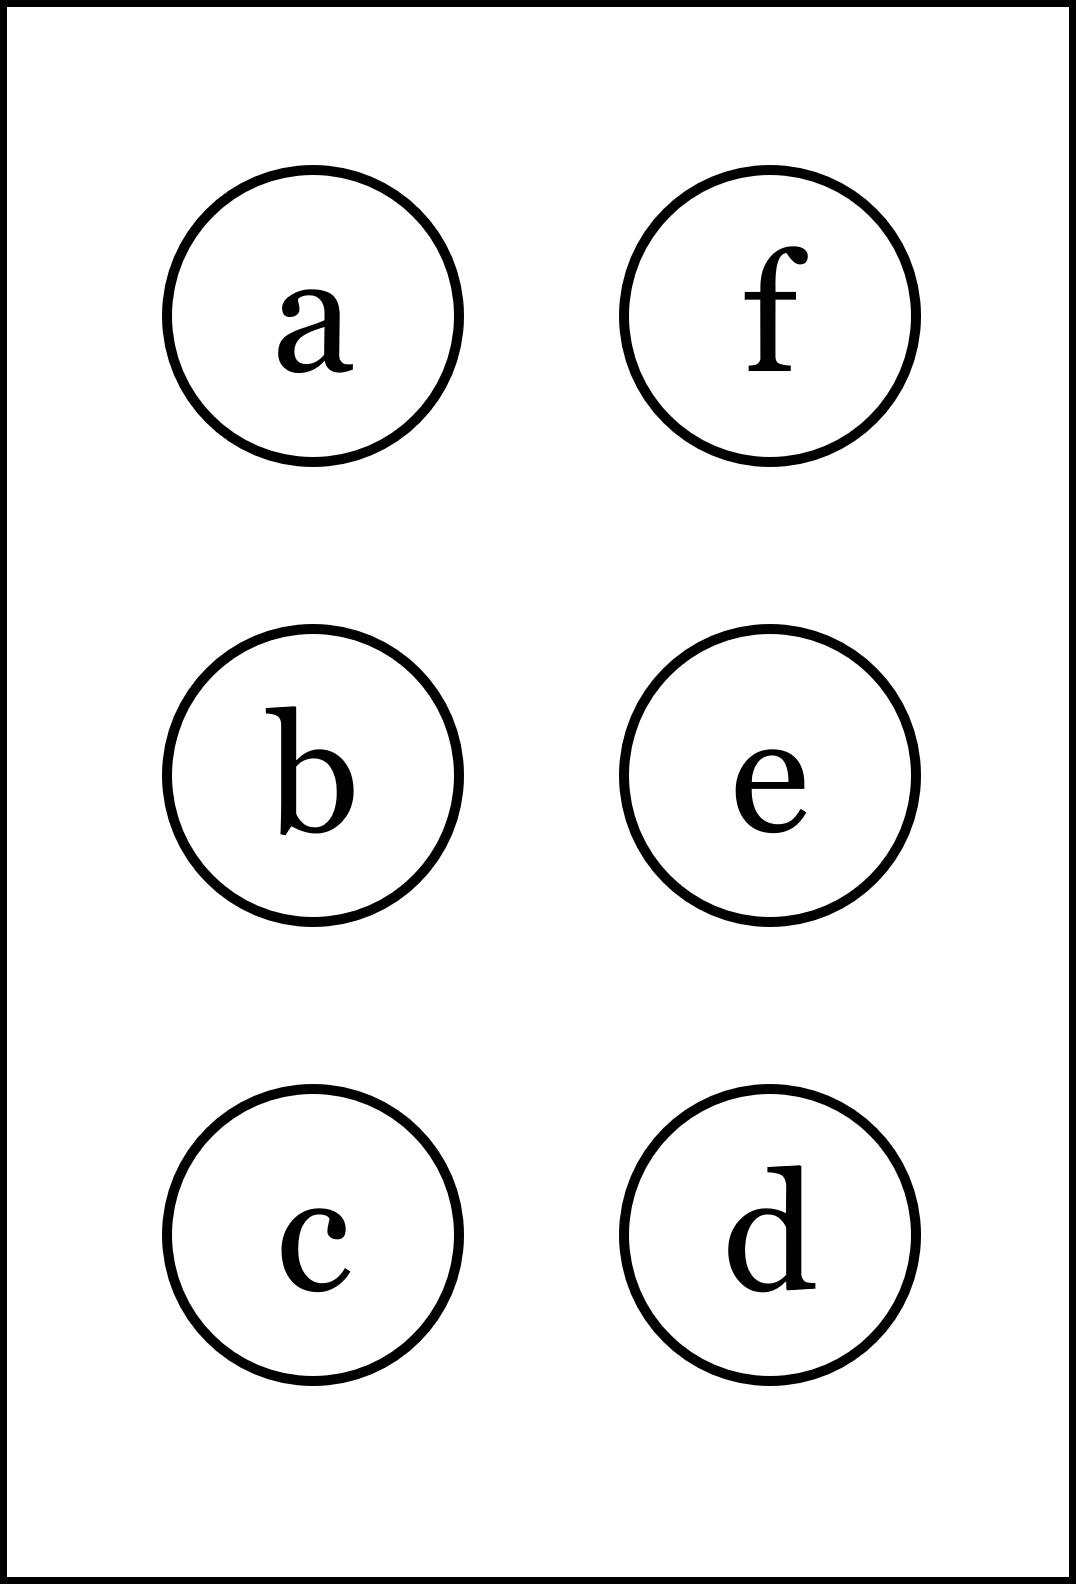
\includegraphics[height=40mm]{../images/braille.png}
{\small Písmeno Braillovej abecedy}
\end{center}
\end{minipage}
\end{center}
\end{minipage}
&
\begin{minipage}[c][104.5mm][t]{0.5\linewidth}
\begin{center}
\vspace{7mm}
{\huge Závorky a zlomky, skupina \textit{Alpha $\alpha$} -\romannumeral2}\\[5mm]
\textit{Jméno:}\phantom{xxxxxxxxxxxxxxxxxxxxxxxxxxxxxxxxxxxxxxxxxxxxxxxxxxxxxxxxxxxxxxxxx}\\[5mm]
\begin{minipage}{0.95\linewidth}
\begin{center}
\textbf{Uprav výrazy (a) až (f)}. Pokud je výraz za otazníky roven výrazu pred otázniky, tak napravo obarvi príslušející kroužek. \textbf{Spolu odevzdejte výsledné slovo.}
\end{center}
\end{minipage}
\\[1mm]
\begin{minipage}{0.79\linewidth}
\begin{center}
\begin{varwidth}{\linewidth}
\begin{enumerate}
\normalsize
\item $6(8x+5)-3(6-x)$\quad \dotfill\; ???\;\dotfill \quad $51x+12$
\item $-4(-3+5x)(-3x+1)+4(9+x)$\quad \dotfill\; ???\;\dotfill \quad $60x^2-52x+48$
\item $(-4x-4)^3-(-6x-7)^2$\quad \dotfill\; ???\;\dotfill \quad $64x^3+228x^2-276x-113$
\item $\cfrac{4x+6}{-3}+2\cfrac{-4+2x}{7}$\quad \dotfill\; ???\;\dotfill \quad $\cfrac{-16x+66}{21}$
\item $\cfrac{\frac{3}{1}-\frac{-1}{x}}{\frac{1}{8}+\frac{-6}{4}}$\quad \dotfill\; ???\;\dotfill \quad $\cfrac{96x+32}{-44x}$
\item $\cfrac{(-1-x)^2+4}{(-2x-1)\cdot\frac{-6}{x}}$\quad \dotfill\; ???\;\dotfill \quad $\cfrac{x^3+2x^2-5x}{-12x+6}$
\end{enumerate}
\end{varwidth}
\end{center}
\end{minipage}
\begin{minipage}{0.20\linewidth}
\begin{center}
{\Huge\bfseries 2.} \\[2mm]
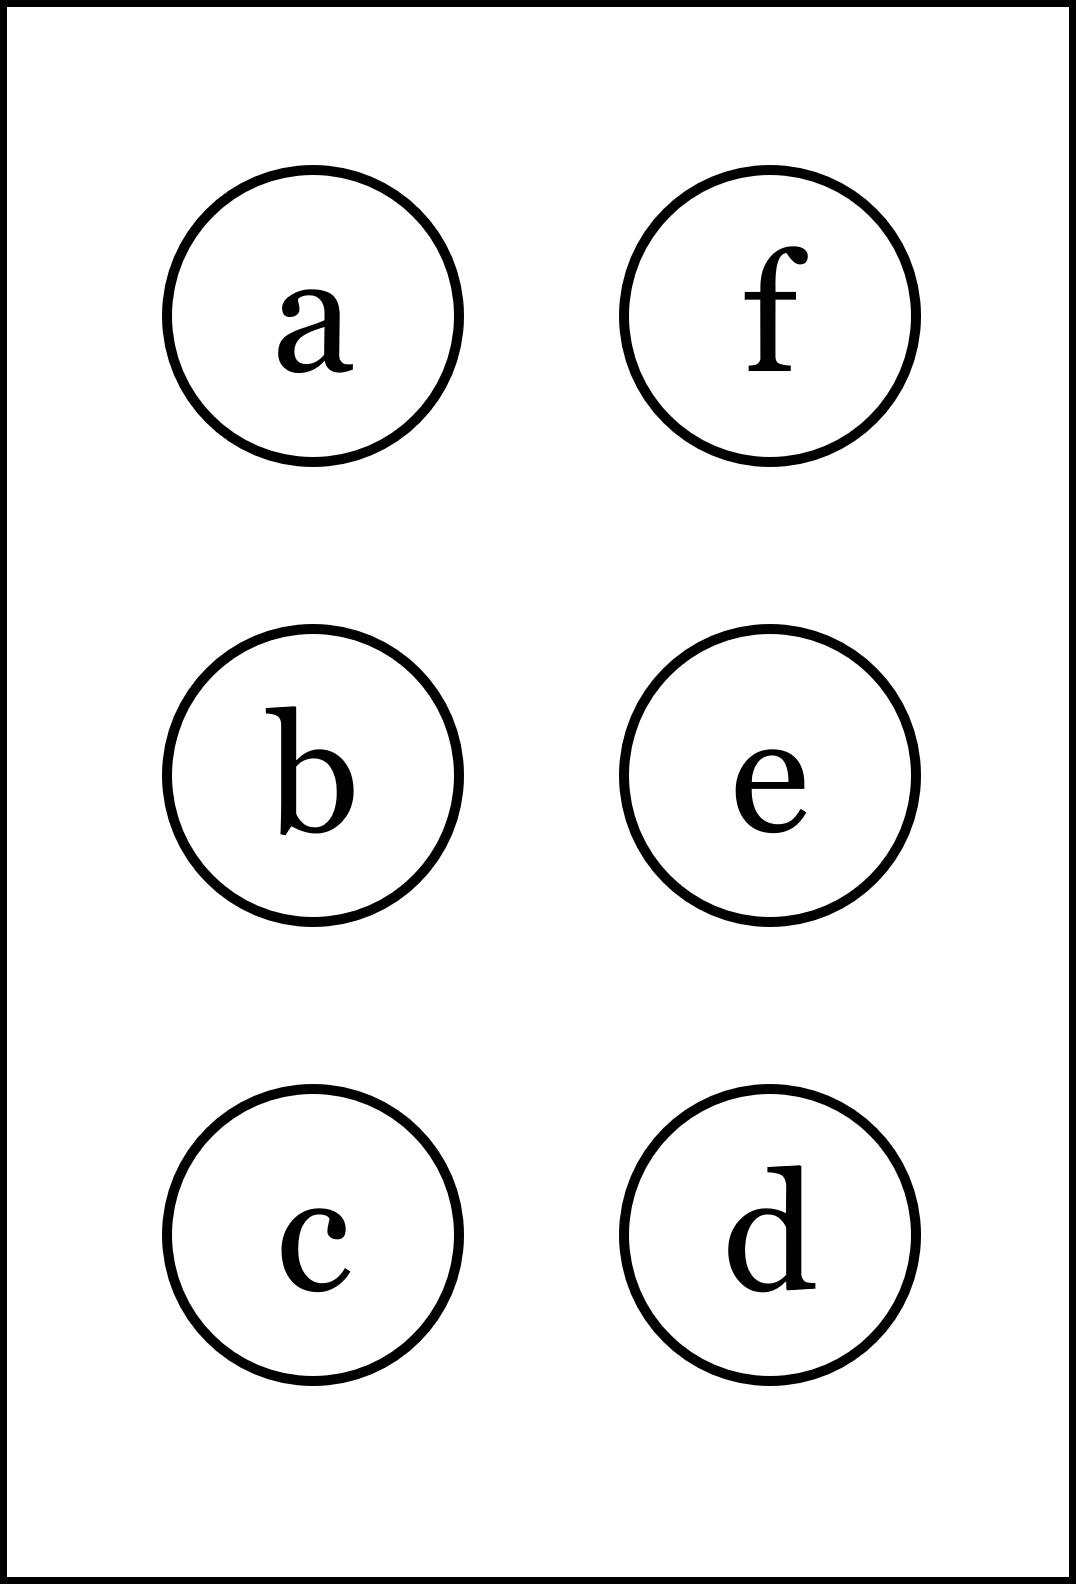
\includegraphics[height=40mm]{../images/braille.png}
{\small Písmeno Braillovej abecedy}
\end{center}
\end{minipage}
\end{center}
\end{minipage}
\\ \hdashline
\begin{minipage}[c][104.5mm][t]{0.5\linewidth}
\begin{center}
\vspace{7mm}
{\huge Závorky a zlomky, skupina \textit{Alpha $\alpha$} -\romannumeral3}\\[5mm]
\textit{Jméno:}\phantom{xxxxxxxxxxxxxxxxxxxxxxxxxxxxxxxxxxxxxxxxxxxxxxxxxxxxxxxxxxxxxxxxx}\\[5mm]
\begin{minipage}{0.95\linewidth}
\begin{center}
\textbf{Uprav výrazy (a) až (f)}. Pokud je výraz za otazníky roven výrazu pred otázniky, tak napravo obarvi príslušející kroužek. \textbf{Spolu odevzdejte výsledné slovo.}
\end{center}
\end{minipage}
\\[1mm]
\begin{minipage}{0.79\linewidth}
\begin{center}
\begin{varwidth}{\linewidth}
\begin{enumerate}
\normalsize
\item $-6(9x-8)-1(-8+3x)$\quad \dotfill\; ???\;\dotfill \quad $-57x+56$
\item $5(-3-6x)(3x-1)-3(1-4x)$\quad \dotfill\; ???\;\dotfill \quad $-90x^2+3x$
\item $(2x+1)^3-(7x+7)^2$\quad \dotfill\; ???\;\dotfill \quad $-8x^3+37x^2-48$
\item $\cfrac{-x+5}{6}+2\cfrac{2-x}{-6}$\quad \dotfill\; ???\;\dotfill \quad $\cfrac{-6x-6}{36}$
\item $\cfrac{\frac{-3}{-4}-\frac{2}{x}}{\frac{1}{-1}+\frac{1}{3}}$\quad \dotfill\; ???\;\dotfill \quad $\cfrac{9x-24}{-8x}$
\item $\cfrac{(-5-x)^2-9}{(x-7)\cdot\frac{6}{x}}$\quad \dotfill\; ???\;\dotfill \quad $\cfrac{x^3+10x^2-16x}{-6x-42}$
\end{enumerate}
\end{varwidth}
\end{center}
\end{minipage}
\begin{minipage}{0.20\linewidth}
\begin{center}
{\Huge\bfseries 3.} \\[2mm]
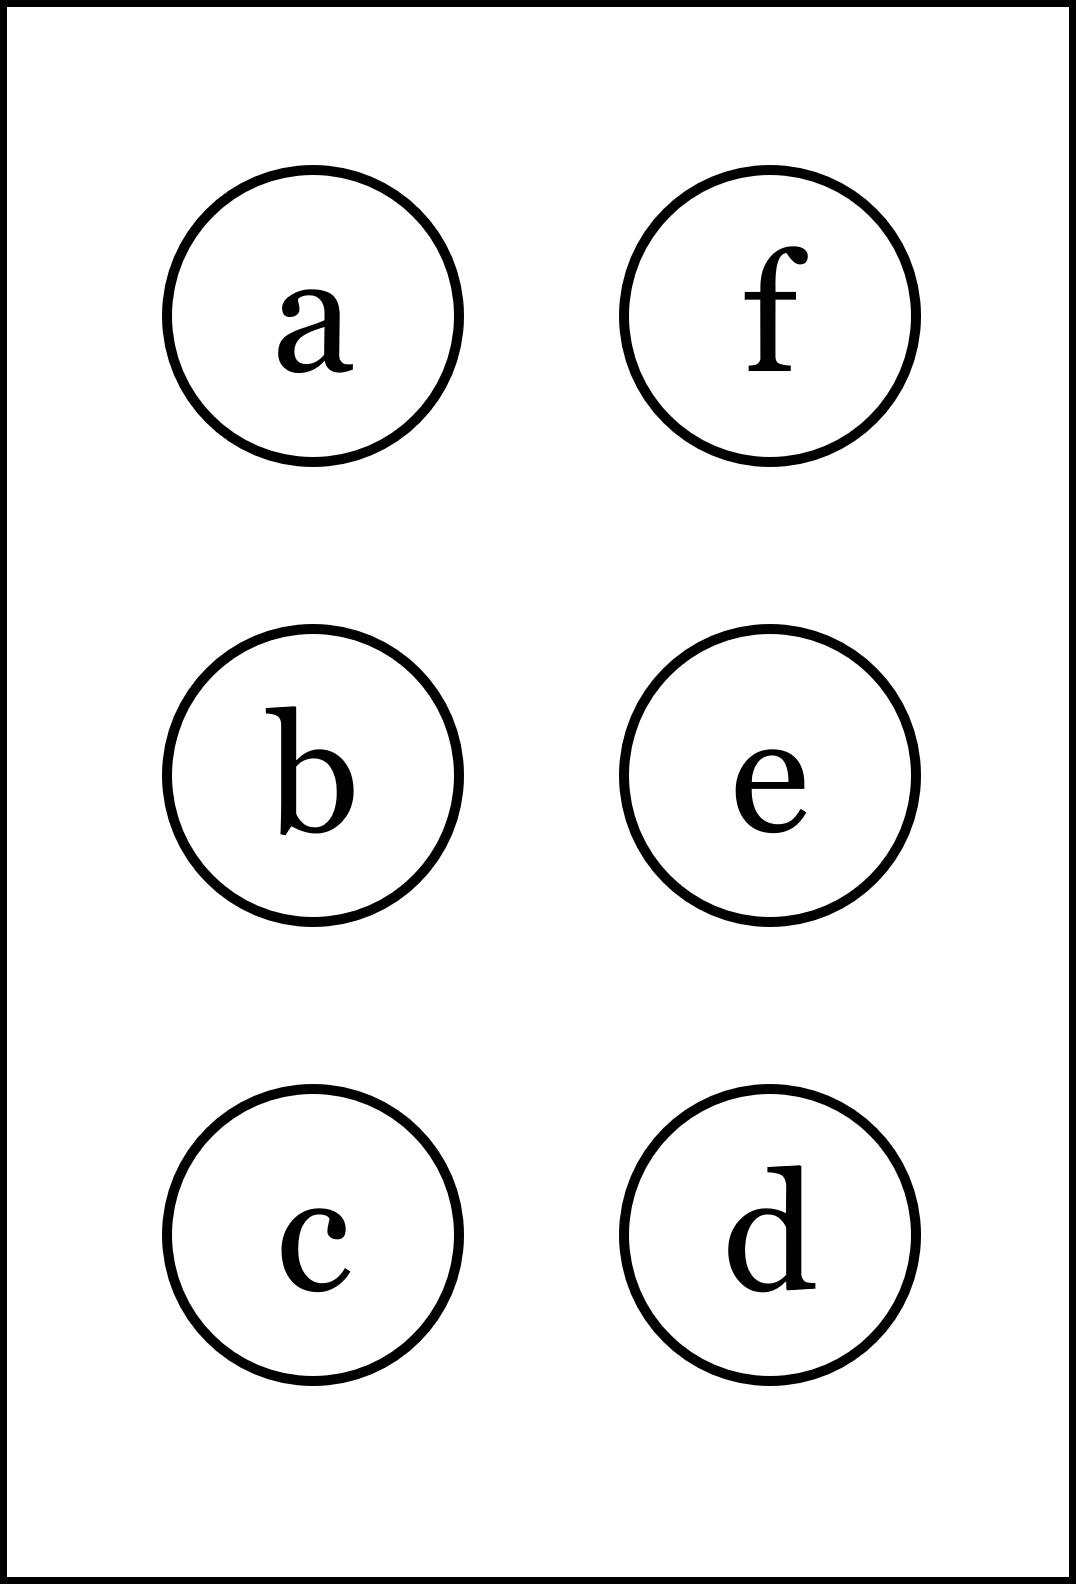
\includegraphics[height=40mm]{../images/braille.png}
{\small Písmeno Braillovej abecedy}
\end{center}
\end{minipage}
\end{center}
\end{minipage}
&
\begin{minipage}[c][104.5mm][t]{0.5\linewidth}
\begin{center}
\vspace{7mm}
{\huge Závorky a zlomky, skupina \textit{Alpha $\alpha$} -\romannumeral4}\\[5mm]
\textit{Jméno:}\phantom{xxxxxxxxxxxxxxxxxxxxxxxxxxxxxxxxxxxxxxxxxxxxxxxxxxxxxxxxxxxxxxxxx}\\[5mm]
\begin{minipage}{0.95\linewidth}
\begin{center}
\textbf{Uprav výrazy (a) až (f)}. Pokud je výraz za otazníky roven výrazu pred otázniky, tak napravo obarvi príslušející kroužek. \textbf{Spolu odevzdejte výsledné slovo.}
\end{center}
\end{minipage}
\\[1mm]
\begin{minipage}{0.79\linewidth}
\begin{center}
\begin{varwidth}{\linewidth}
\begin{enumerate}
\normalsize
\item $-5(-5x+4)-3(-5-2x)$\quad \dotfill\; ???\;\dotfill \quad $31x-5$
\item $2(3-5x)(-x+5)-2(8+6x)$\quad \dotfill\; ???\;\dotfill \quad $10x^2-68x+14$
\item $(-x-3)^3-(-2x-5)^2$\quad \dotfill\; ???\;\dotfill \quad $-x^3-13x^2-47x-52$
\item $\cfrac{-7x+4}{3}+3\cfrac{2-x}{7}$\quad \dotfill\; ???\;\dotfill \quad $\cfrac{58x+46}{-21}$
\item $\cfrac{\frac{5}{8}-\frac{-2}{x}}{\frac{1}{3}+\frac{1}{-2}}$\quad \dotfill\; ???\;\dotfill \quad $\cfrac{-27x-97}{8x}$
\item $\cfrac{(4+2x)^2-2}{(-6x+6)\cdot\frac{5}{x}}$\quad \dotfill\; ???\;\dotfill \quad $\cfrac{4x^3+16x^2-14x}{30x+30}$
\end{enumerate}
\end{varwidth}
\end{center}
\end{minipage}
\begin{minipage}{0.20\linewidth}
\begin{center}
{\Huge\bfseries 4.} \\[2mm]
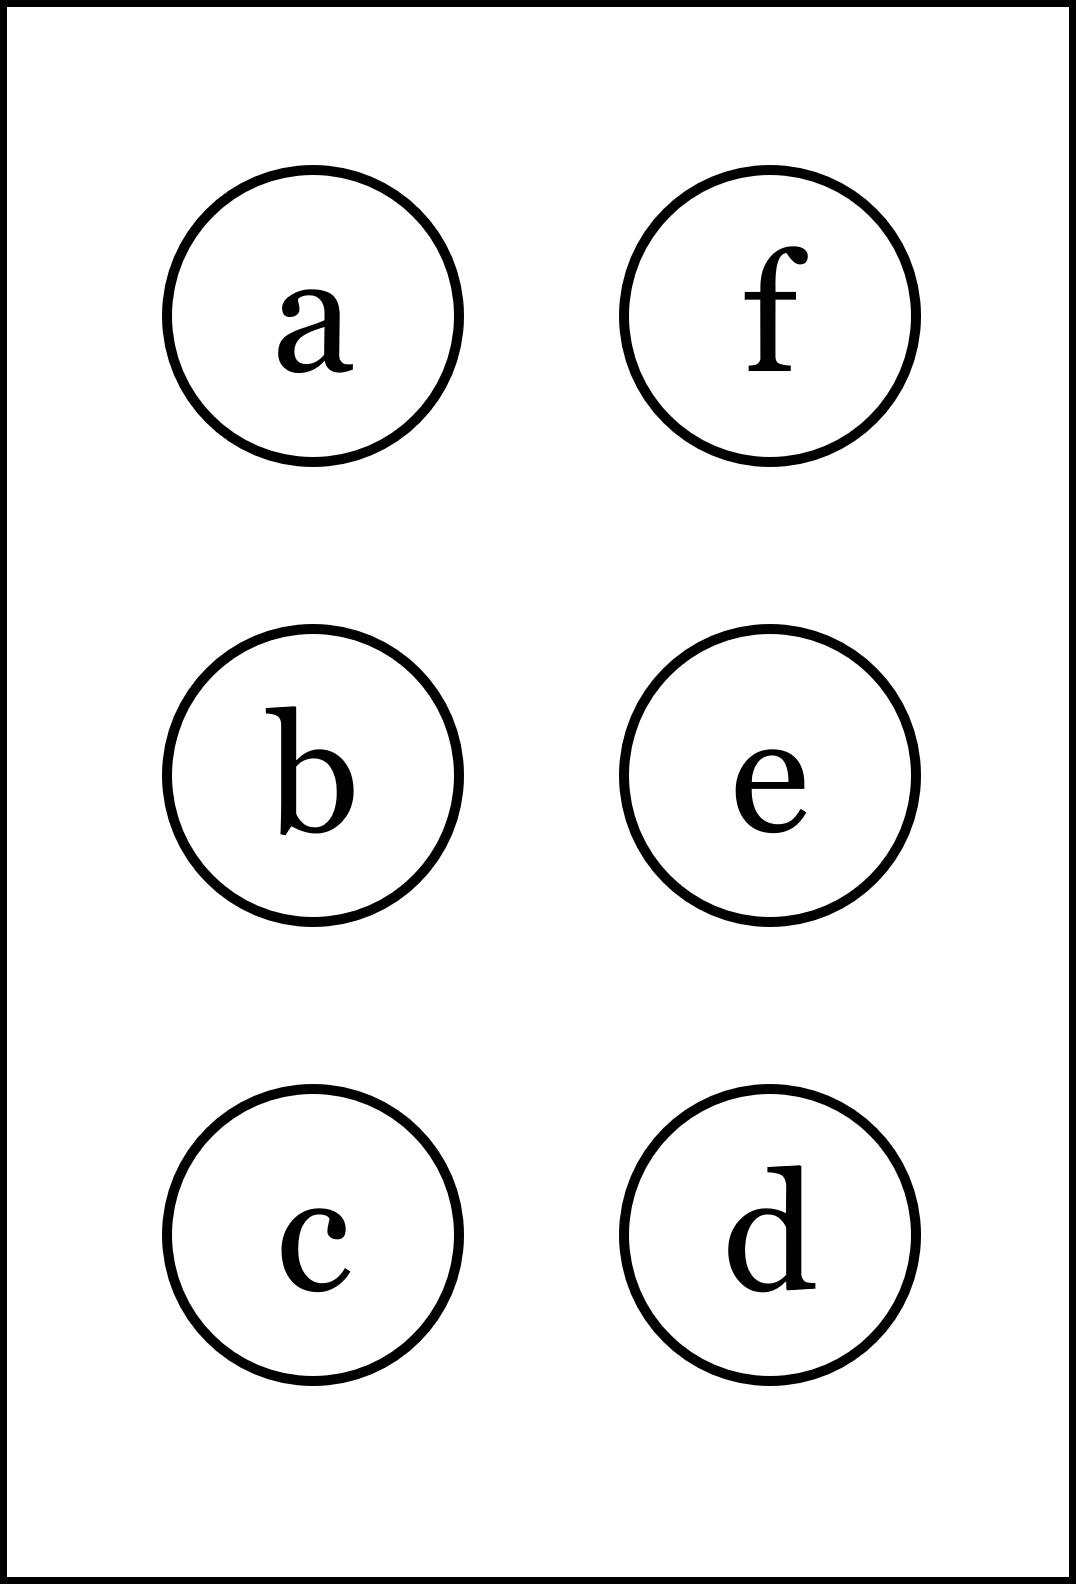
\includegraphics[height=40mm]{../images/braille.png}
{\small Písmeno Braillovej abecedy}
\end{center}
\end{minipage}
\end{center}
\end{minipage}
%
\end{tabular}
\newpage
\thispagestyle{empty}
\begin{tabular}{c:c}
\begin{minipage}[c][104.5mm][t]{0.5\linewidth}
\begin{center}
\vspace{7mm}
{\huge Závorky a zlomky, skupina \textit{Beta $\beta$} -\romannumeral1}\\[5mm]
\textit{Jméno:}\phantom{xxxxxxxxxxxxxxxxxxxxxxxxxxxxxxxxxxxxxxxxxxxxxxxxxxxxxxxxxxxxxxxxx}\\[5mm]
\begin{minipage}{0.95\linewidth}
\begin{center}
\textbf{Uprav výrazy (a) až (f)}. Pokud je výraz za otazníky roven výrazu pred otázniky, tak napravo obarvi príslušející kroužek. \textbf{Spolu odevzdejte výsledné slovo.}
\end{center}
\end{minipage}
\\[1mm]
\begin{minipage}{0.79\linewidth}
\begin{center}
\begin{varwidth}{\linewidth}
\begin{enumerate}
\normalsize
\item $-6(-5x+9)-4(-1+3x)$\quad \dotfill\; ???\;\dotfill \quad $18x+50$
\item $-2(8-5x)(-2x+2)-6(-2+7x)$\quad \dotfill\; ???\;\dotfill \quad $-20x^2+10x-20$
\item $(-x-1)^3-(6x+2)^2$\quad \dotfill\; ???\;\dotfill \quad $-x^3-39x^2-27x-5$
\item $\cfrac{-4x-4}{3}+5\cfrac{-3+3x}{-2}$\quad \dotfill\; ???\;\dotfill \quad $\cfrac{53x-37}{6}$
\item $\cfrac{\frac{-2}{-2}-\frac{1}{x}}{\frac{1}{4}+\frac{3}{6}}$\quad \dotfill\; ???\;\dotfill \quad $\cfrac{-45x+50}{-36x}$
\item $\cfrac{(-3+4x)^2-6}{(-2x-5)\cdot\frac{1}{x}}$\quad \dotfill\; ???\;\dotfill \quad $\cfrac{16x^3-24x^2+3x}{-2x-5}$
\end{enumerate}
\end{varwidth}
\end{center}
\end{minipage}
\begin{minipage}{0.20\linewidth}
\begin{center}
{\Huge\bfseries 1.} \\[2mm]
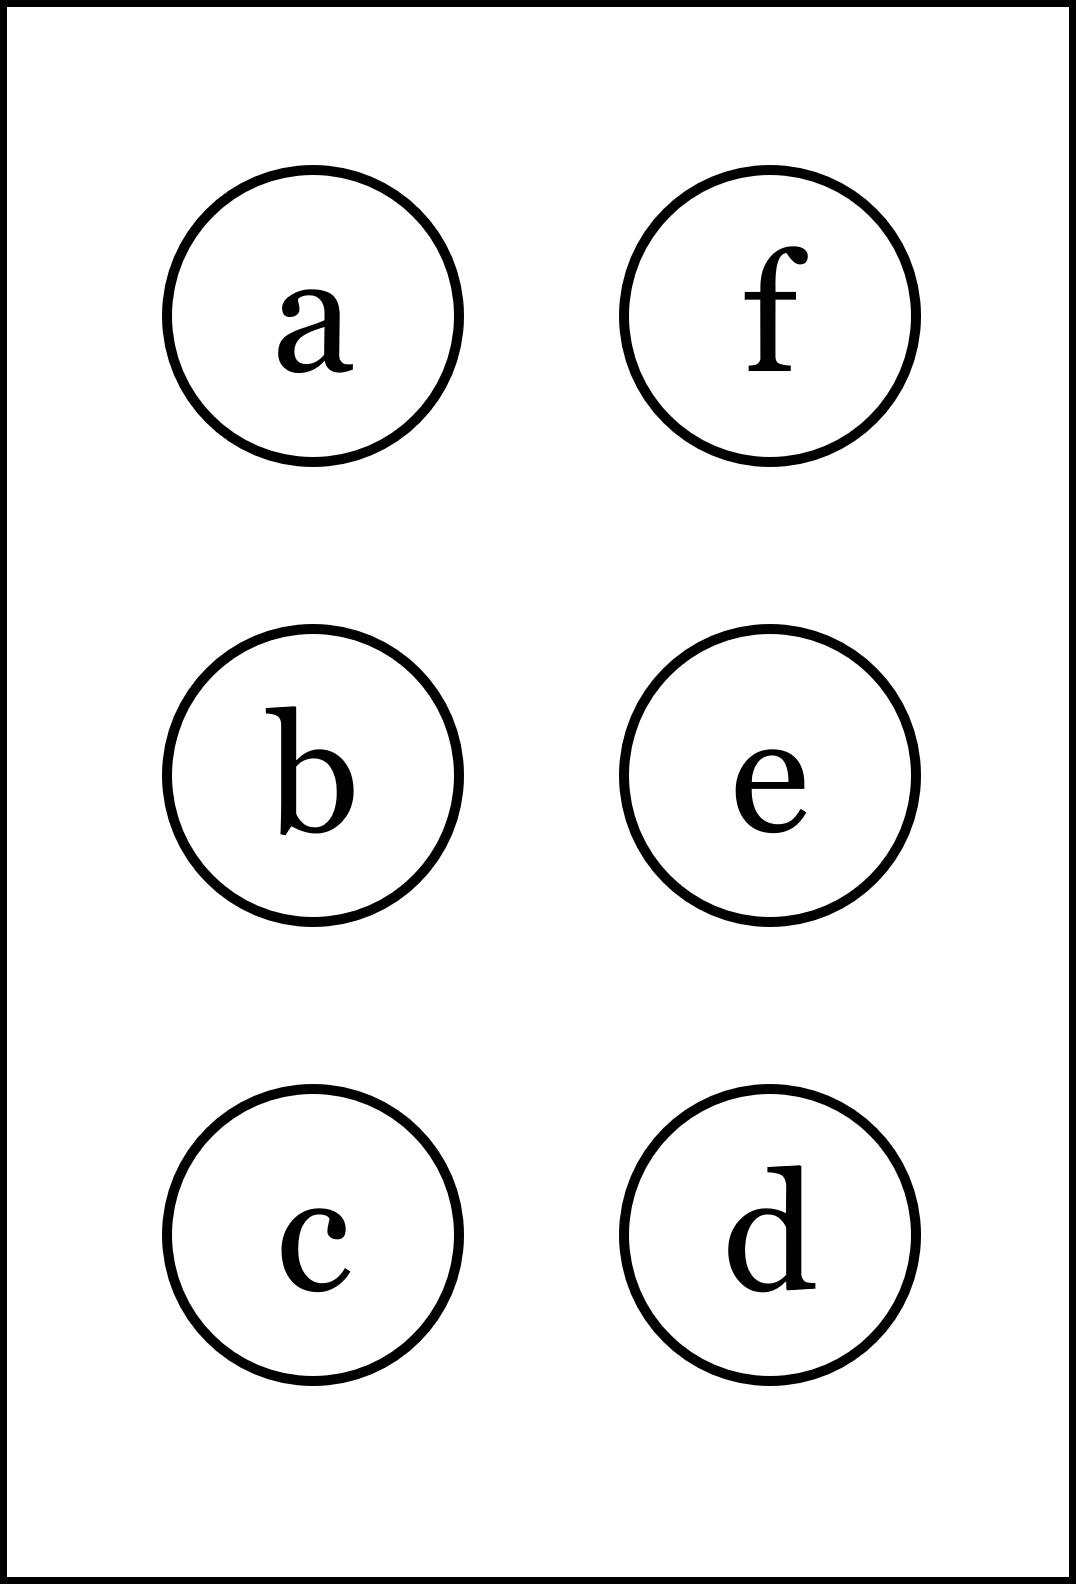
\includegraphics[height=40mm]{../images/braille.png}
{\small Písmeno Braillovej abecedy}
\end{center}
\end{minipage}
\end{center}
\end{minipage}
&
\begin{minipage}[c][104.5mm][t]{0.5\linewidth}
\begin{center}
\vspace{7mm}
{\huge Závorky a zlomky, skupina \textit{Beta $\beta$} -\romannumeral2}\\[5mm]
\textit{Jméno:}\phantom{xxxxxxxxxxxxxxxxxxxxxxxxxxxxxxxxxxxxxxxxxxxxxxxxxxxxxxxxxxxxxxxxx}\\[5mm]
\begin{minipage}{0.95\linewidth}
\begin{center}
\textbf{Uprav výrazy (a) až (f)}. Pokud je výraz za otazníky roven výrazu pred otázniky, tak napravo obarvi príslušející kroužek. \textbf{Spolu odevzdejte výsledné slovo.}
\end{center}
\end{minipage}
\\[1mm]
\begin{minipage}{0.79\linewidth}
\begin{center}
\begin{varwidth}{\linewidth}
\begin{enumerate}
\normalsize
\item $-4(-3x+1)-3(8-2x)$\quad \dotfill\; ???\;\dotfill \quad $18x-28$
\item $3(4-3x)(x-4)-2(4+2x)$\quad \dotfill\; ???\;\dotfill \quad $-9x^2+44x-56$
\item $(3x+2)^3-(-8x-5)^2$\quad \dotfill\; ???\;\dotfill \quad $27x^3-10x^2-44x-17$
\item $\cfrac{3x+5}{3}-3\cfrac{-2+2x}{4}$\quad \dotfill\; ???\;\dotfill \quad $\cfrac{-6x+38}{-12}$
\item $\cfrac{\frac{3}{3}-\frac{1}{x}}{\frac{1}{3}+\frac{-5}{-2}}$\quad \dotfill\; ???\;\dotfill \quad $\cfrac{-19x+17}{-51x}$
\item $\cfrac{(-7+8x)^2+6}{(-4x-2)\cdot\frac{1}{x}}$\quad \dotfill\; ???\;\dotfill \quad $\cfrac{64x^3-112x^2-55x}{4x-2}$
\end{enumerate}
\end{varwidth}
\end{center}
\end{minipage}
\begin{minipage}{0.20\linewidth}
\begin{center}
{\Huge\bfseries 2.} \\[2mm]
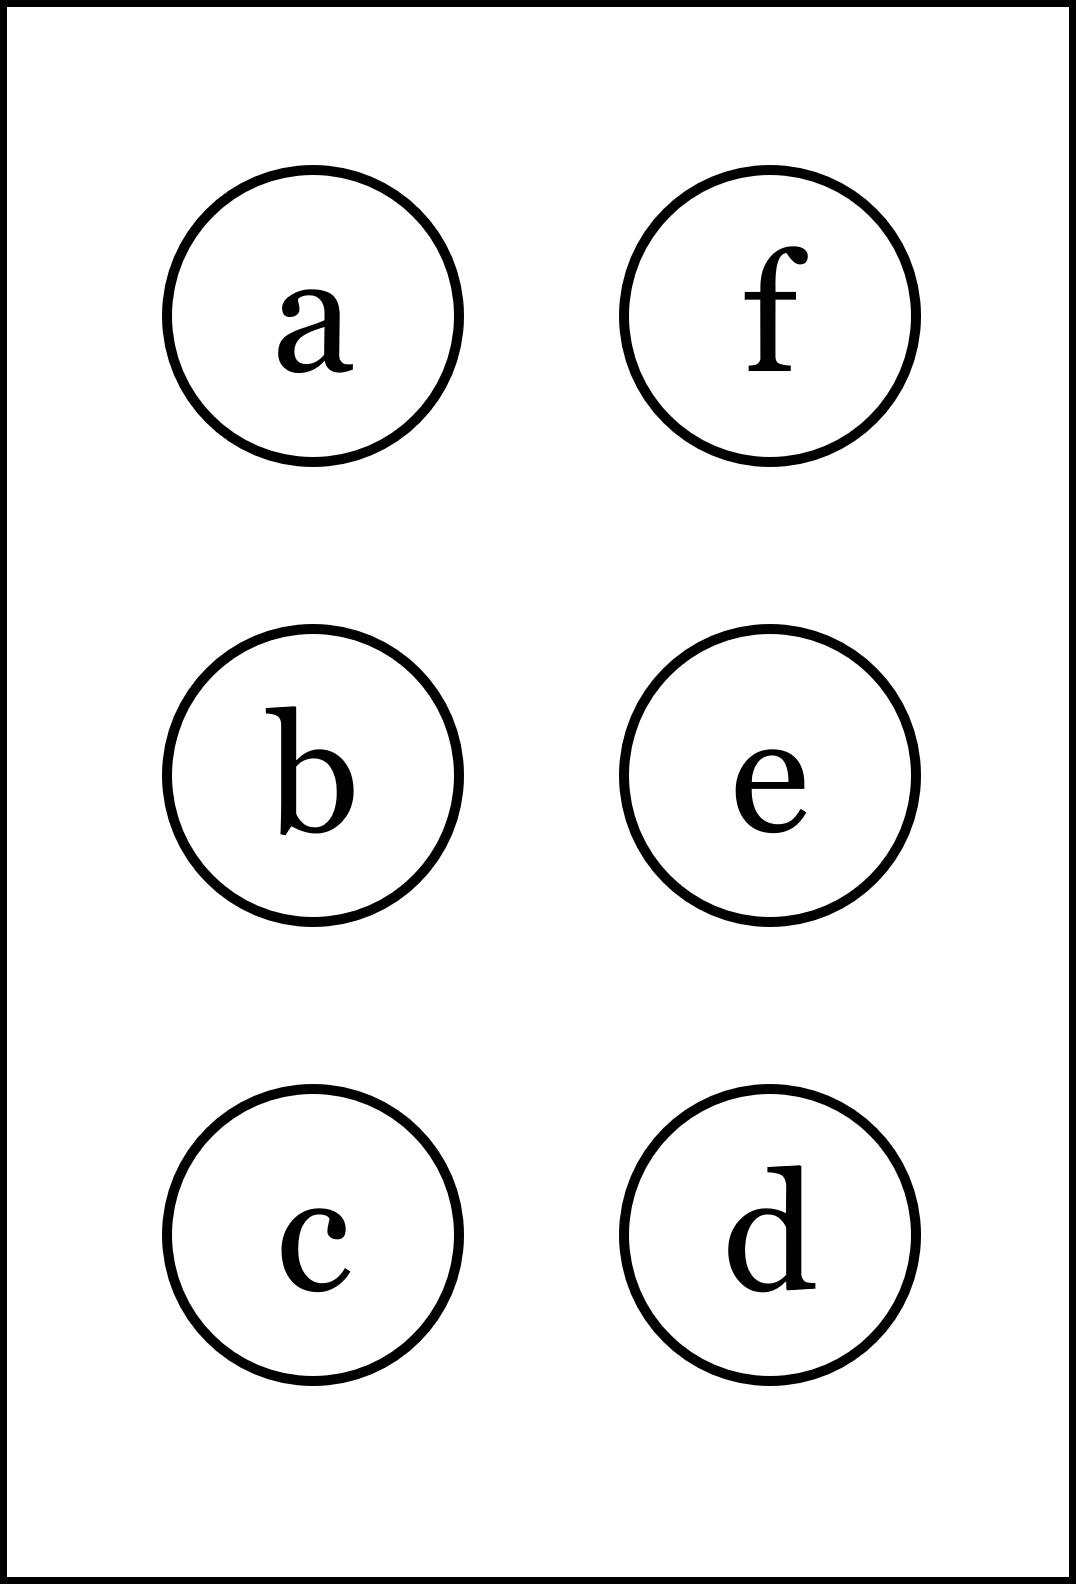
\includegraphics[height=40mm]{../images/braille.png}
{\small Písmeno Braillovej abecedy}
\end{center}
\end{minipage}
\end{center}
\end{minipage}
\\ \hdashline
\begin{minipage}[c][104.5mm][t]{0.5\linewidth}
\begin{center}
\vspace{7mm}
{\huge Závorky a zlomky, skupina \textit{Beta $\beta$} -\romannumeral3}\\[5mm]
\textit{Jméno:}\phantom{xxxxxxxxxxxxxxxxxxxxxxxxxxxxxxxxxxxxxxxxxxxxxxxxxxxxxxxxxxxxxxxxx}\\[5mm]
\begin{minipage}{0.95\linewidth}
\begin{center}
\textbf{Uprav výrazy (a) až (f)}. Pokud je výraz za otazníky roven výrazu pred otázniky, tak napravo obarvi príslušející kroužek. \textbf{Spolu odevzdejte výsledné slovo.}
\end{center}
\end{minipage}
\\[1mm]
\begin{minipage}{0.79\linewidth}
\begin{center}
\begin{varwidth}{\linewidth}
\begin{enumerate}
\normalsize
\item $-7(9x+2)+6(-1+x)$\quad \dotfill\; ???\;\dotfill \quad $-57x-20$
\item $-2(2+5x)(3x+3)-3(-9+3x)$\quad \dotfill\; ???\;\dotfill \quad $-30x^2+51x-15$
\item $(-4x-1)^3-(-3x-2)^2$\quad \dotfill\; ???\;\dotfill \quad $-64x^3-57x^2-24x-5$
\item $\cfrac{-3x+6}{-4}+4\cfrac{3-2x}{5}$\quad \dotfill\; ???\;\dotfill \quad $\cfrac{17x-18}{20}$
\item $\cfrac{\frac{-2}{-1}-\frac{-1}{x}}{\frac{1}{7}+\frac{-6}{-1}}$\quad \dotfill\; ???\;\dotfill \quad $\cfrac{14x+7}{43x}$
\item $\cfrac{(-4-6x)^2+5}{(2x-2)\cdot\frac{-6}{x}}$\quad \dotfill\; ???\;\dotfill \quad $\cfrac{36x^3+48x^2-21x}{12x+12}$
\end{enumerate}
\end{varwidth}
\end{center}
\end{minipage}
\begin{minipage}{0.20\linewidth}
\begin{center}
{\Huge\bfseries 3.} \\[2mm]
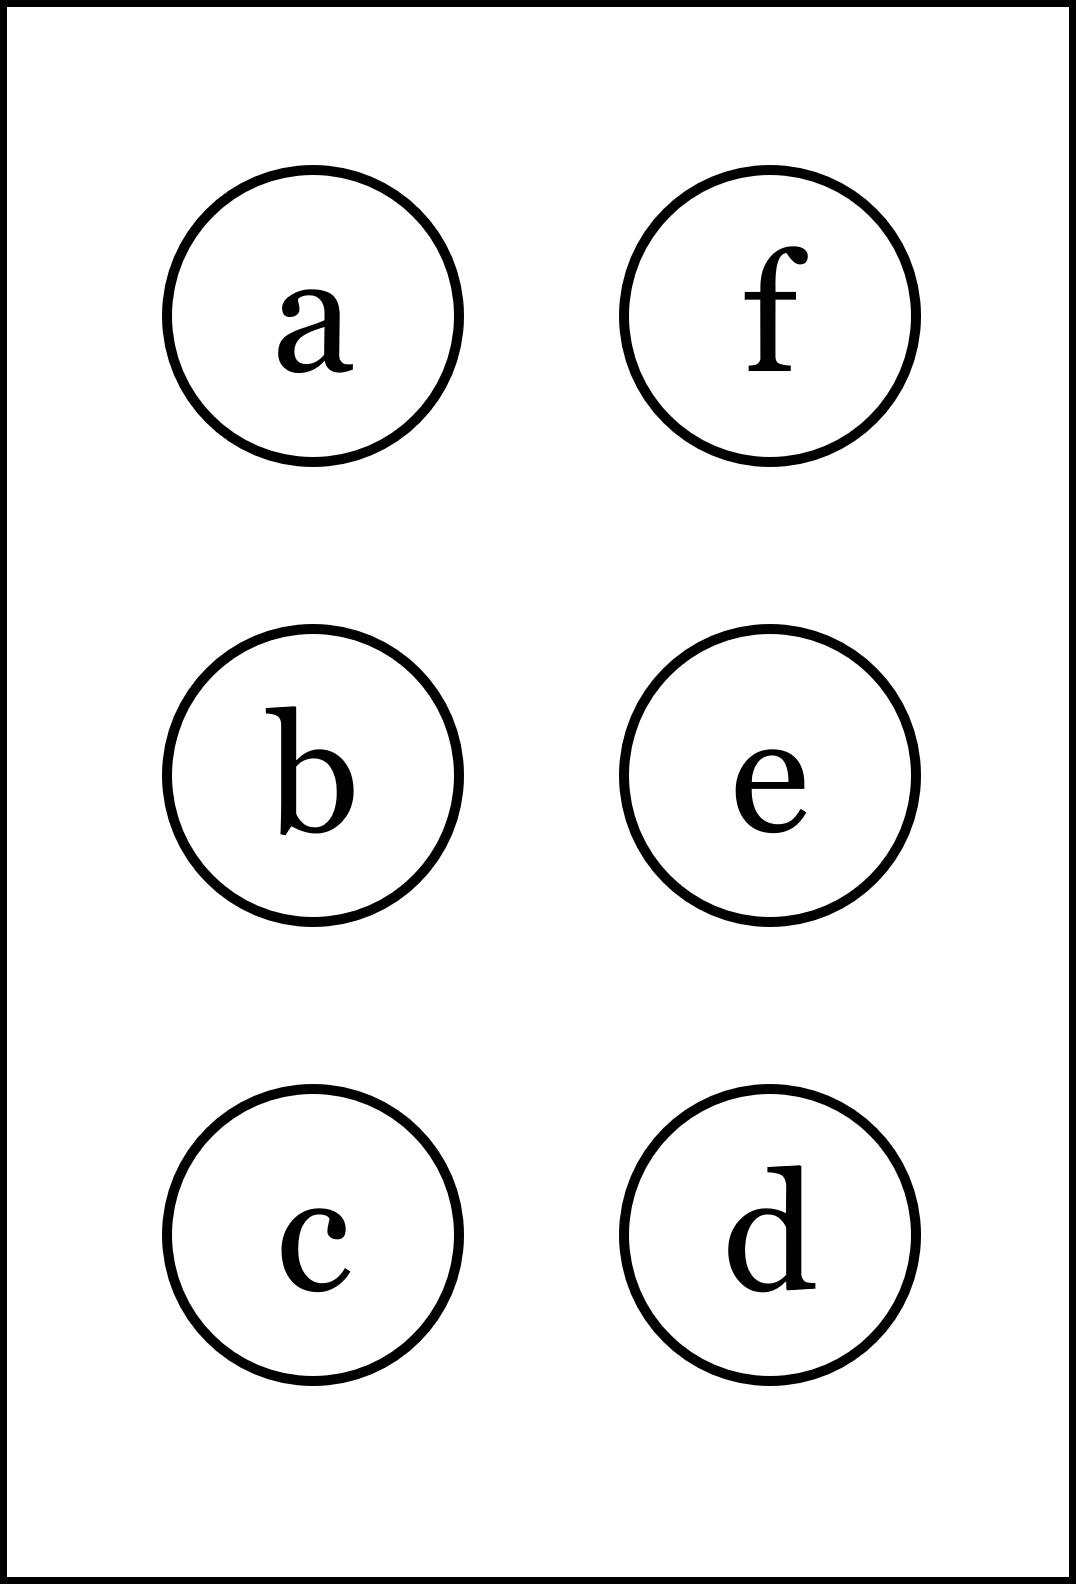
\includegraphics[height=40mm]{../images/braille.png}
{\small Písmeno Braillovej abecedy}
\end{center}
\end{minipage}
\end{center}
\end{minipage}
&
\begin{minipage}[c][104.5mm][t]{0.5\linewidth}
\begin{center}
\vspace{7mm}
{\huge Závorky a zlomky, skupina \textit{Beta $\beta$} -\romannumeral4}\\[5mm]
\textit{Jméno:}\phantom{xxxxxxxxxxxxxxxxxxxxxxxxxxxxxxxxxxxxxxxxxxxxxxxxxxxxxxxxxxxxxxxxx}\\[5mm]
\begin{minipage}{0.95\linewidth}
\begin{center}
\textbf{Uprav výrazy (a) až (f)}. Pokud je výraz za otazníky roven výrazu pred otázniky, tak napravo obarvi príslušející kroužek. \textbf{Spolu odevzdejte výsledné slovo.}
\end{center}
\end{minipage}
\\[1mm]
\begin{minipage}{0.79\linewidth}
\begin{center}
\begin{varwidth}{\linewidth}
\begin{enumerate}
\normalsize
\item $-4(-6x-2)-9(4-x)$\quad \dotfill\; ???\;\dotfill \quad $33x-28$
\item $-2(4-2x)(-x+5)-3(-7+9x)$\quad \dotfill\; ???\;\dotfill \quad $-4x^2-x+19$
\item $(2x-3)^3-(-7x+9)^2$\quad \dotfill\; ???\;\dotfill \quad $8x^3-85x^2+180x-108$
\item $\cfrac{x+8}{5}-3\cfrac{-2-3x}{-5}$\quad \dotfill\; ???\;\dotfill \quad $\cfrac{-40x-10}{25}$
\item $\cfrac{\frac{2}{-3}-\frac{-2}{x}}{\frac{1}{4}+\frac{-3}{-3}}$\quad \dotfill\; ???\;\dotfill \quad $\cfrac{-24x+72}{45x}$
\item $\cfrac{(1+x)^2-9}{(5x+4)\cdot\frac{-4}{x}}$\quad \dotfill\; ???\;\dotfill \quad $\cfrac{x^3+2x^2-8x}{-20x-16}$
\end{enumerate}
\end{varwidth}
\end{center}
\end{minipage}
\begin{minipage}{0.20\linewidth}
\begin{center}
{\Huge\bfseries 4.} \\[2mm]
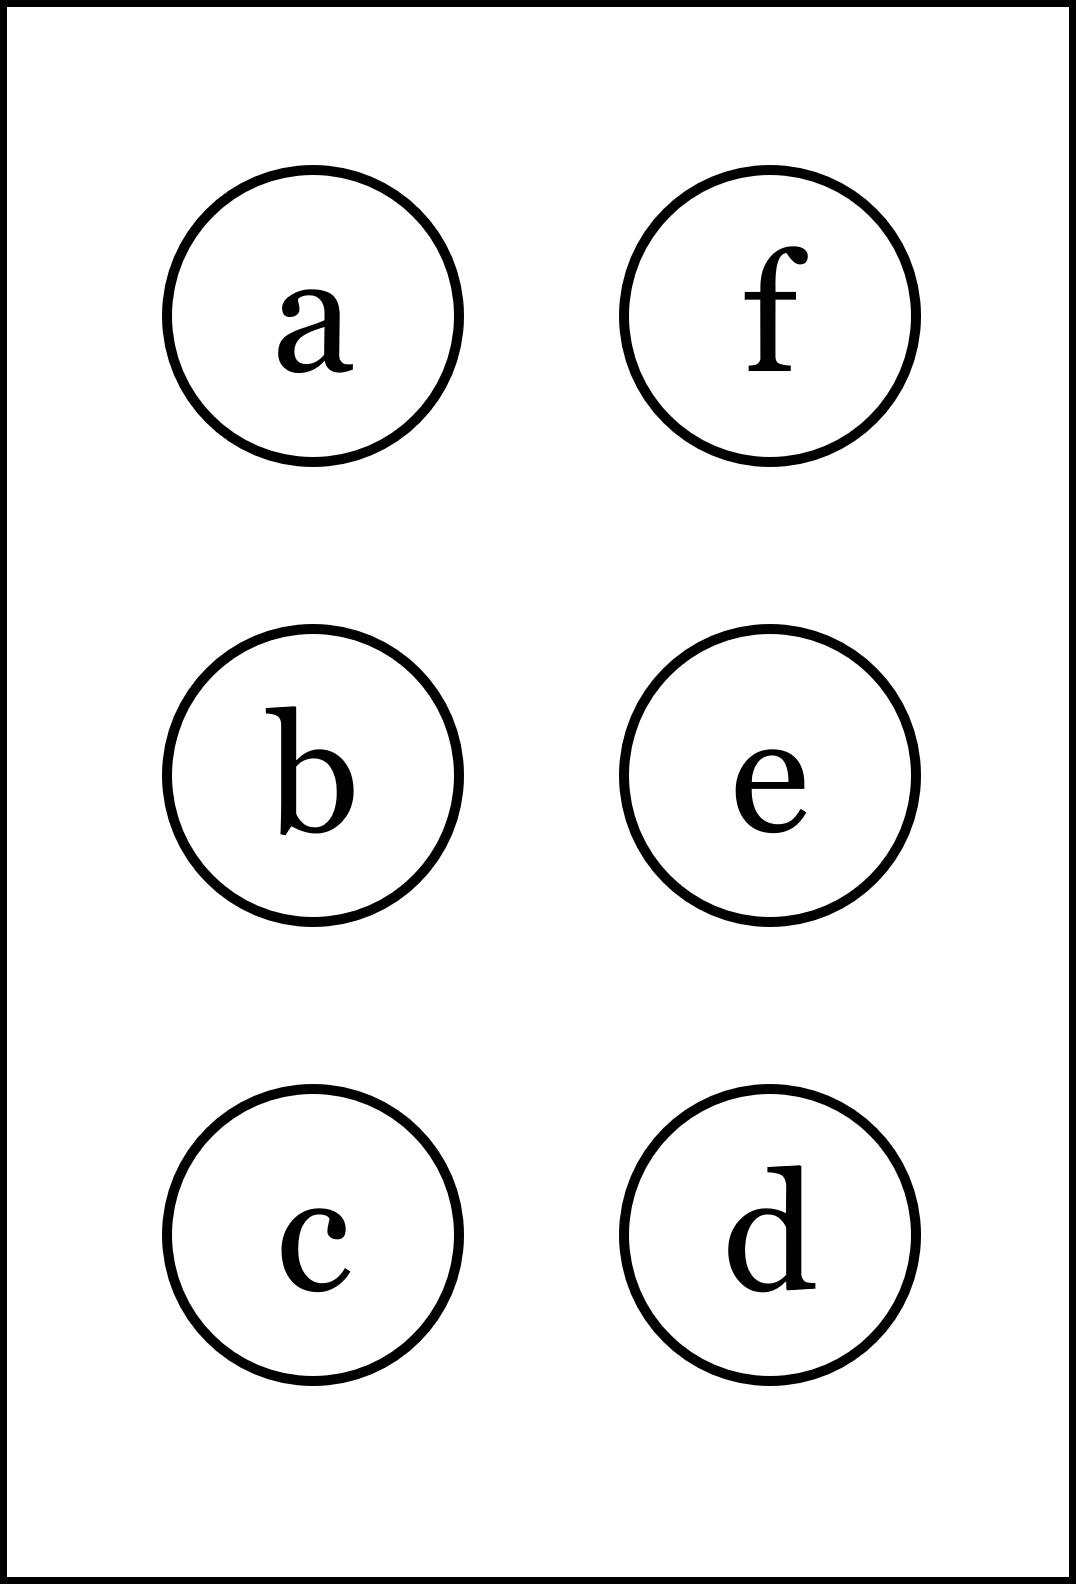
\includegraphics[height=40mm]{../images/braille.png}
{\small Písmeno Braillovej abecedy}
\end{center}
\end{minipage}
\end{center}
\end{minipage}
%
\end{tabular}
\newpage
\thispagestyle{empty}
\begin{tabular}{c:c}
\begin{minipage}[c][104.5mm][t]{0.5\linewidth}
\begin{center}
\vspace{7mm}
{\huge Závorky a zlomky, skupina \textit{Gamma $\gamma$} -\romannumeral1}\\[5mm]
\textit{Jméno:}\phantom{xxxxxxxxxxxxxxxxxxxxxxxxxxxxxxxxxxxxxxxxxxxxxxxxxxxxxxxxxxxxxxxxx}\\[5mm]
\begin{minipage}{0.95\linewidth}
\begin{center}
\textbf{Uprav výrazy (a) až (f)}. Pokud je výraz za otazníky roven výrazu pred otázniky, tak napravo obarvi príslušející kroužek. \textbf{Spolu odevzdejte výsledné slovo.}
\end{center}
\end{minipage}
\\[1mm]
\begin{minipage}{0.79\linewidth}
\begin{center}
\begin{varwidth}{\linewidth}
\begin{enumerate}
\normalsize
\item $6(4x+3)-3(-2-3x)$\quad \dotfill\; ???\;\dotfill \quad $33x-24$
\item $3(-6-6x)(-3x+2)-1(5-7x)$\quad \dotfill\; ???\;\dotfill \quad $54x^2-25x+41$
\item $(2x-1)^3-(5x+6)^2$\quad \dotfill\; ???\;\dotfill \quad $8x^3-37x^2-54x-37$
\item $\cfrac{-x+1}{5}-2\cfrac{2+7x}{-6}$\quad \dotfill\; ???\;\dotfill \quad $\cfrac{-64x-26}{-30}$
\item $\cfrac{\frac{-5}{8}-\frac{-2}{x}}{\frac{1}{-4}+\frac{2}{1}}$\quad \dotfill\; ???\;\dotfill \quad $\cfrac{19x-62}{-56x}$
\item $\cfrac{(-6-2x)^2+4}{(2x-9)\cdot\frac{-5}{x}}$\quad \dotfill\; ???\;\dotfill \quad $\cfrac{4x^3+24x^2+40x}{-10x+45}$
\end{enumerate}
\end{varwidth}
\end{center}
\end{minipage}
\begin{minipage}{0.20\linewidth}
\begin{center}
{\Huge\bfseries 1.} \\[2mm]
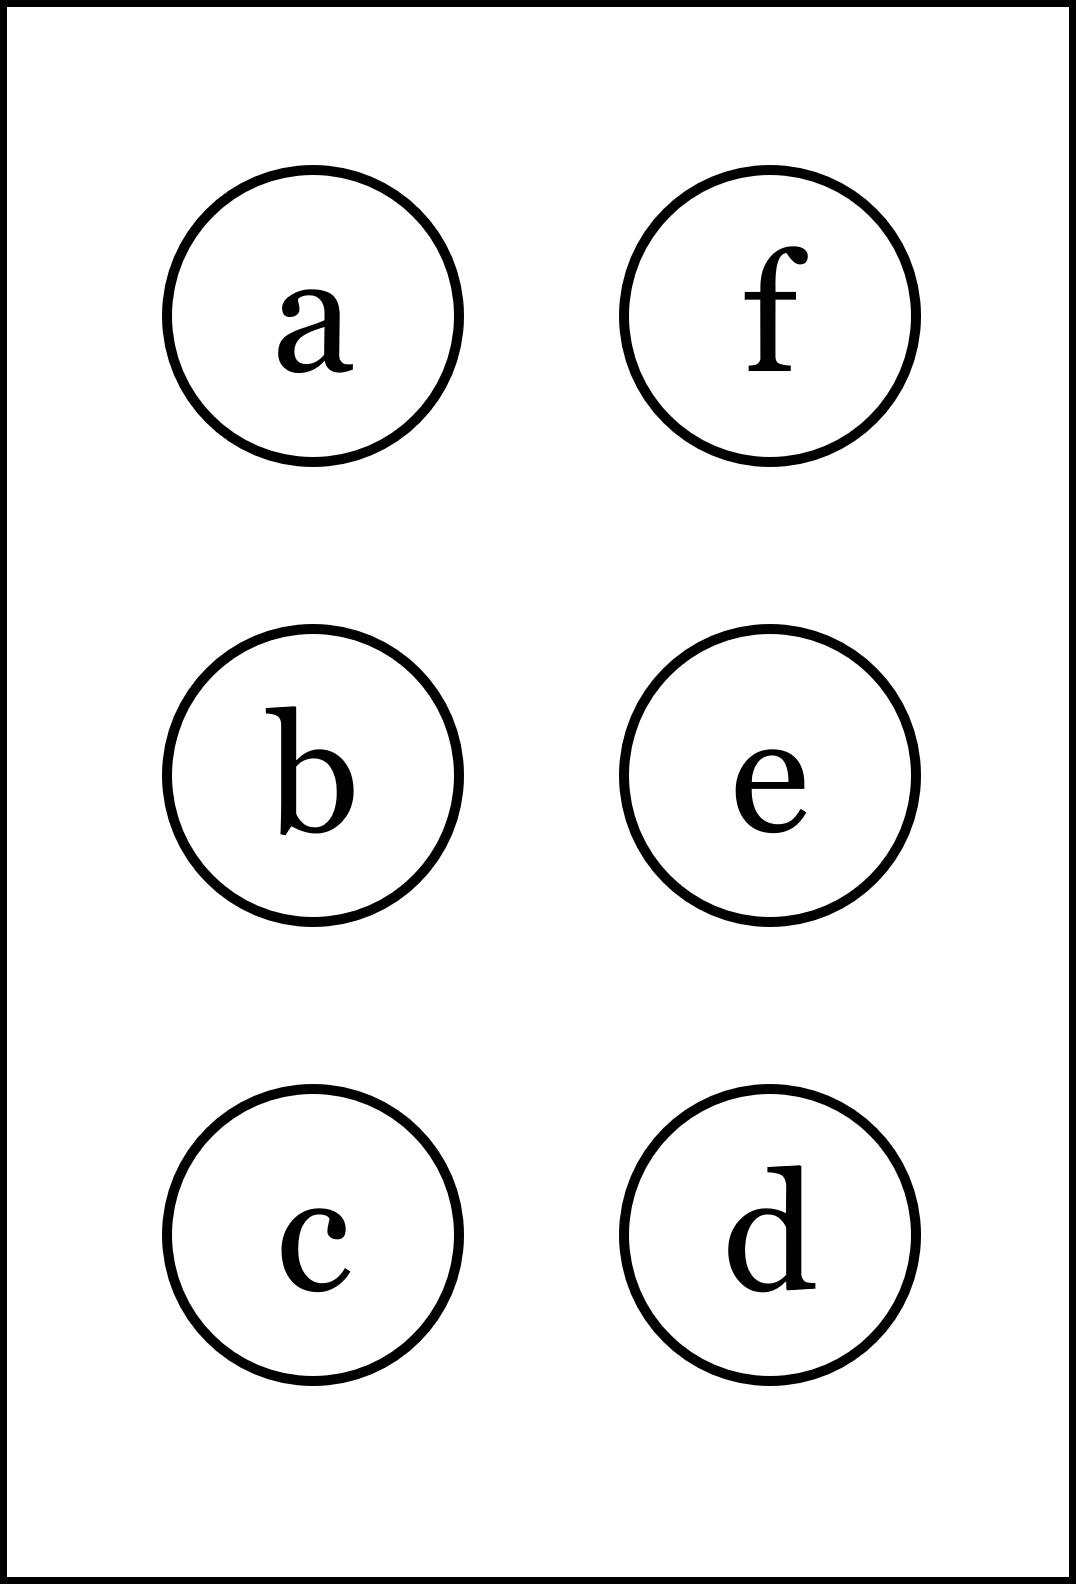
\includegraphics[height=40mm]{../images/braille.png}
{\small Písmeno Braillovej abecedy}
\end{center}
\end{minipage}
\end{center}
\end{minipage}
&
\begin{minipage}[c][104.5mm][t]{0.5\linewidth}
\begin{center}
\vspace{7mm}
{\huge Závorky a zlomky, skupina \textit{Gamma $\gamma$} -\romannumeral2}\\[5mm]
\textit{Jméno:}\phantom{xxxxxxxxxxxxxxxxxxxxxxxxxxxxxxxxxxxxxxxxxxxxxxxxxxxxxxxxxxxxxxxxx}\\[5mm]
\begin{minipage}{0.95\linewidth}
\begin{center}
\textbf{Uprav výrazy (a) až (f)}. Pokud je výraz za otazníky roven výrazu pred otázniky, tak napravo obarvi príslušející kroužek. \textbf{Spolu odevzdejte výsledné slovo.}
\end{center}
\end{minipage}
\\[1mm]
\begin{minipage}{0.79\linewidth}
\begin{center}
\begin{varwidth}{\linewidth}
\begin{enumerate}
\normalsize
\item $-7(3x-2)+3(-3+6x)$\quad \dotfill\; ???\;\dotfill \quad $-3x+5$
\item $5(4+2x)(2x-4)+5(6-x)$\quad \dotfill\; ???\;\dotfill \quad $20x^2+5x$
\item $(-x+2)^3-(-3x+6)^2$\quad \dotfill\; ???\;\dotfill \quad $-x^3-3x^2+24x-28$
\item $\cfrac{-2x-1}{-3}-4\cfrac{-4+5x}{3}$\quad \dotfill\; ???\;\dotfill \quad $\cfrac{-51}{9}$
\item $\cfrac{\frac{4}{4}-\frac{3}{x}}{\frac{1}{8}+\frac{1}{1}}$\quad \dotfill\; ???\;\dotfill \quad $\cfrac{31x-94}{36x}$
\item $\cfrac{(3+x)^2+7}{(3x-2)\cdot\frac{-3}{x}}$\quad \dotfill\; ???\;\dotfill \quad $\cfrac{x^3+6x^2-16x}{9x+6}$
\end{enumerate}
\end{varwidth}
\end{center}
\end{minipage}
\begin{minipage}{0.20\linewidth}
\begin{center}
{\Huge\bfseries 2.} \\[2mm]
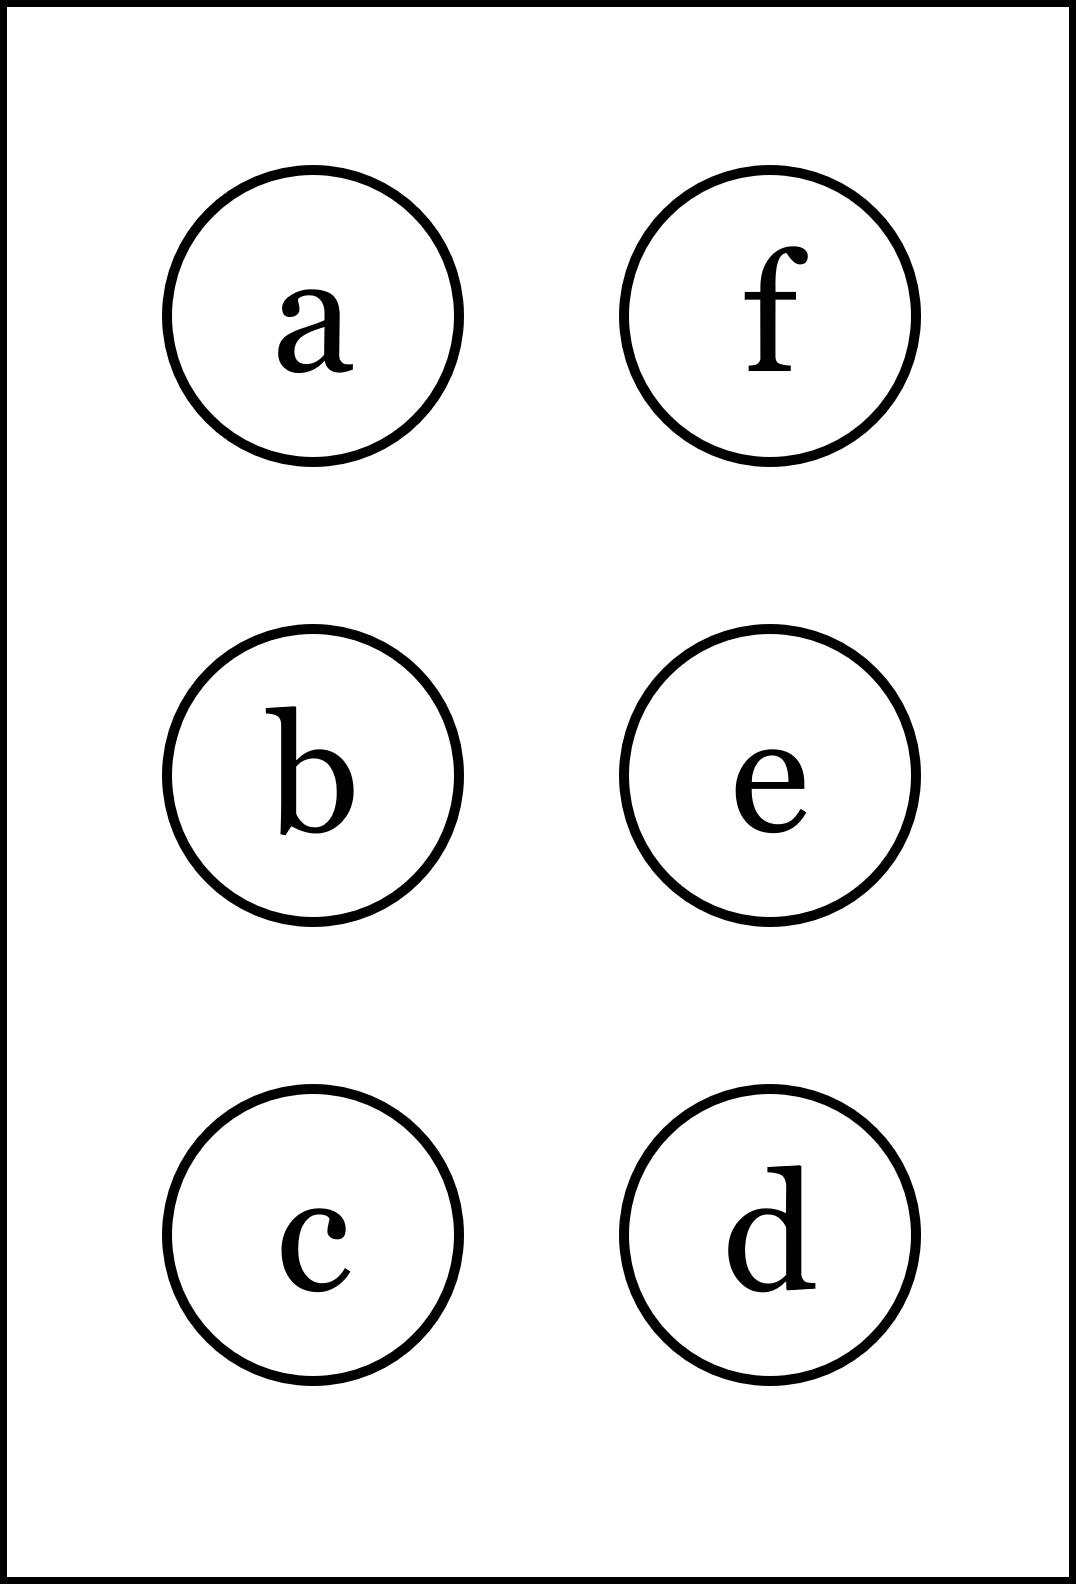
\includegraphics[height=40mm]{../images/braille.png}
{\small Písmeno Braillovej abecedy}
\end{center}
\end{minipage}
\end{center}
\end{minipage}
\\ \hdashline
\begin{minipage}[c][104.5mm][t]{0.5\linewidth}
\begin{center}
\vspace{7mm}
{\huge Závorky a zlomky, skupina \textit{Gamma $\gamma$} -\romannumeral3}\\[5mm]
\textit{Jméno:}\phantom{xxxxxxxxxxxxxxxxxxxxxxxxxxxxxxxxxxxxxxxxxxxxxxxxxxxxxxxxxxxxxxxxx}\\[5mm]
\begin{minipage}{0.95\linewidth}
\begin{center}
\textbf{Uprav výrazy (a) až (f)}. Pokud je výraz za otazníky roven výrazu pred otázniky, tak napravo obarvi príslušející kroužek. \textbf{Spolu odevzdejte výsledné slovo.}
\end{center}
\end{minipage}
\\[1mm]
\begin{minipage}{0.79\linewidth}
\begin{center}
\begin{varwidth}{\linewidth}
\begin{enumerate}
\normalsize
\item $4(7x+1)+3(-9+8x)$\quad \dotfill\; ???\;\dotfill \quad $52x-23$
\item $5(-2+4x)(-4x+4)-1(3-7x)$\quad \dotfill\; ???\;\dotfill \quad $-80x^2-127x+43$
\item $(3x-1)^3-(x-6)^2$\quad \dotfill\; ???\;\dotfill \quad $27x^3-28x^2+21x-37$
\item $\cfrac{-8x+4}{-2}+4\cfrac{-6-3x}{6}$\quad \dotfill\; ???\;\dotfill \quad $\cfrac{72}{12}$
\item $\cfrac{\frac{-4}{1}-\frac{-2}{x}}{\frac{1}{-2}+\frac{3}{4}}$\quad \dotfill\; ???\;\dotfill \quad $\cfrac{32x-16}{-2x}$
\item $\cfrac{(-6+x)^2-1}{(-4x+5)\cdot\frac{-3}{x}}$\quad \dotfill\; ???\;\dotfill \quad $\cfrac{x^3-12x^2-35x}{-12x-15}$
\end{enumerate}
\end{varwidth}
\end{center}
\end{minipage}
\begin{minipage}{0.20\linewidth}
\begin{center}
{\Huge\bfseries 3.} \\[2mm]
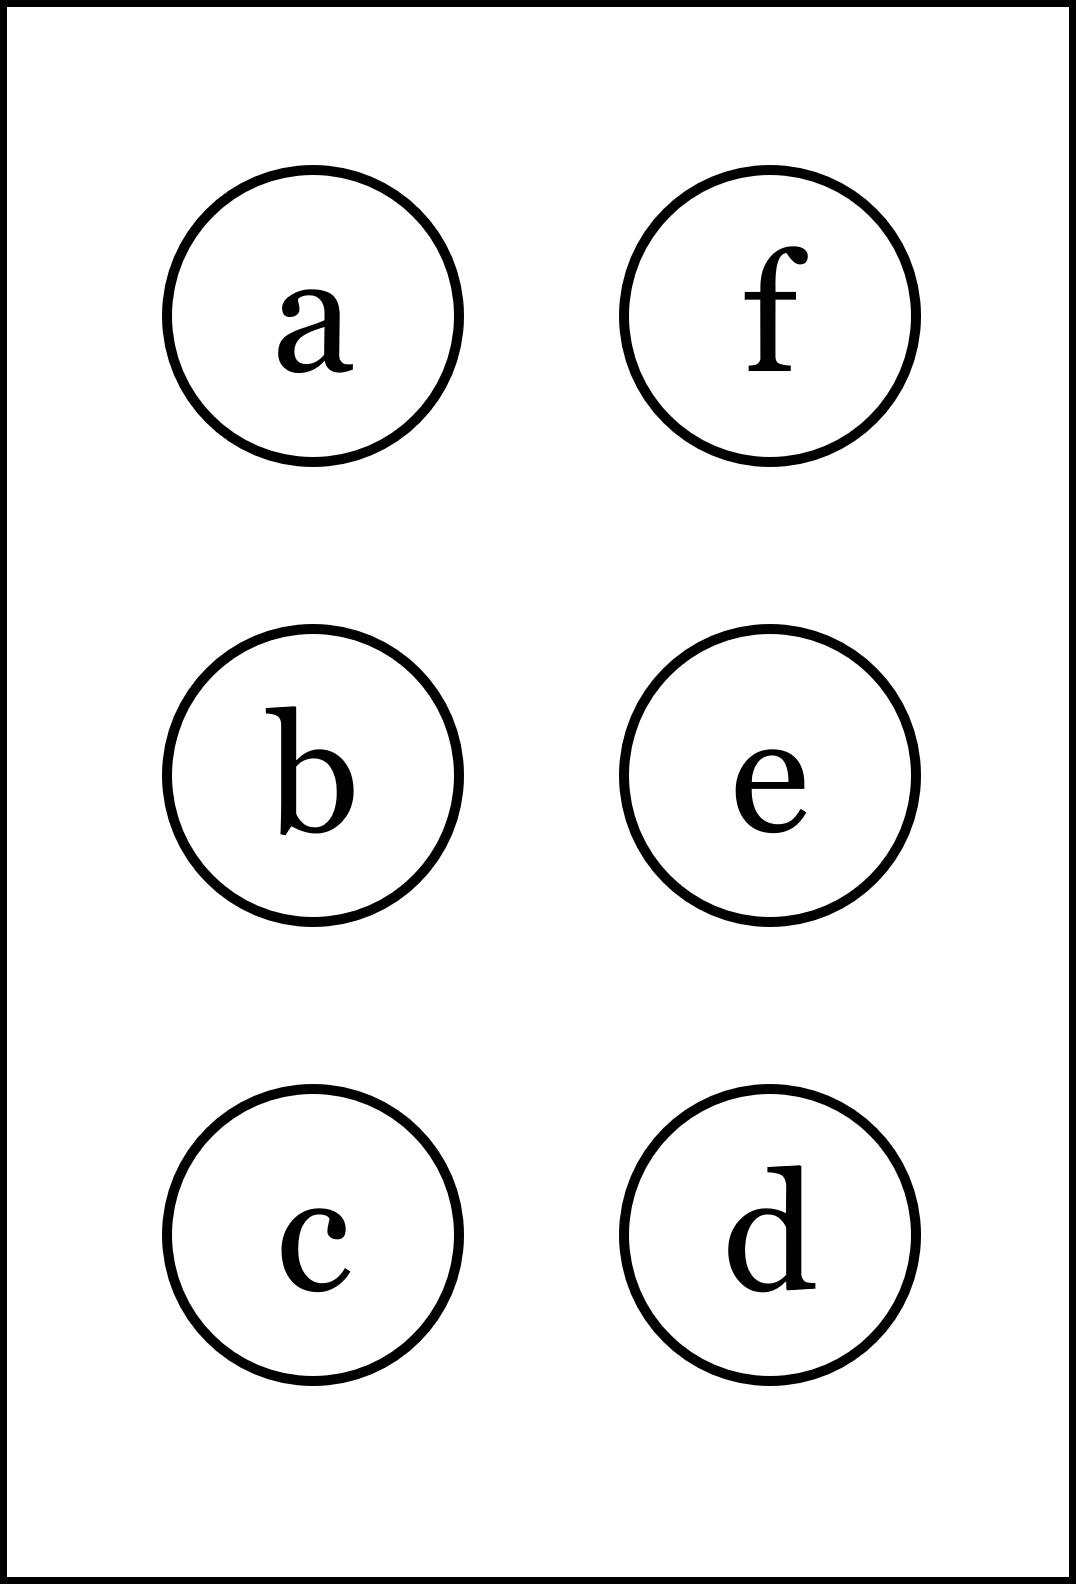
\includegraphics[height=40mm]{../images/braille.png}
{\small Písmeno Braillovej abecedy}
\end{center}
\end{minipage}
\end{center}
\end{minipage}
&
\begin{minipage}[c][104.5mm][t]{0.5\linewidth}
\begin{center}
\vspace{7mm}
{\huge Závorky a zlomky, skupina \textit{Gamma $\gamma$} -\romannumeral4}\\[5mm]
\textit{Jméno:}\phantom{xxxxxxxxxxxxxxxxxxxxxxxxxxxxxxxxxxxxxxxxxxxxxxxxxxxxxxxxxxxxxxxxx}\\[5mm]
\begin{minipage}{0.95\linewidth}
\begin{center}
\textbf{Uprav výrazy (a) až (f)}. Pokud je výraz za otazníky roven výrazu pred otázniky, tak napravo obarvi príslušející kroužek. \textbf{Spolu odevzdejte výsledné slovo.}
\end{center}
\end{minipage}
\\[1mm]
\begin{minipage}{0.79\linewidth}
\begin{center}
\begin{varwidth}{\linewidth}
\begin{enumerate}
\normalsize
\item $-7(-6x-5)+7(-1+4x)$\quad \dotfill\; ???\;\dotfill \quad $70x+28$
\item $-2(8+x)(6x+4)+4(4+6x)$\quad \dotfill\; ???\;\dotfill \quad $-12x^2-80x-48$
\item $(-4x+4)^3-(4x+9)^2$\quad \dotfill\; ???\;\dotfill \quad $-64x^3+176x^2-264x-17$
\item $\cfrac{-3x-3}{2}+5\cfrac{5-7x}{-5}$\quad \dotfill\; ???\;\dotfill \quad $\cfrac{55x+65}{10}$
\item $\cfrac{\frac{1}{-2}-\frac{-1}{x}}{\frac{1}{3}+\frac{5}{-1}}$\quad \dotfill\; ???\;\dotfill \quad $\cfrac{-6x+8}{-28x}$
\item $\cfrac{(1-5x)^2+3}{(x-2)\cdot\frac{5}{x}}$\quad \dotfill\; ???\;\dotfill \quad $\cfrac{25x^3-10x^2-4x}{-5x-10}$
\end{enumerate}
\end{varwidth}
\end{center}
\end{minipage}
\begin{minipage}{0.20\linewidth}
\begin{center}
{\Huge\bfseries 4.} \\[2mm]
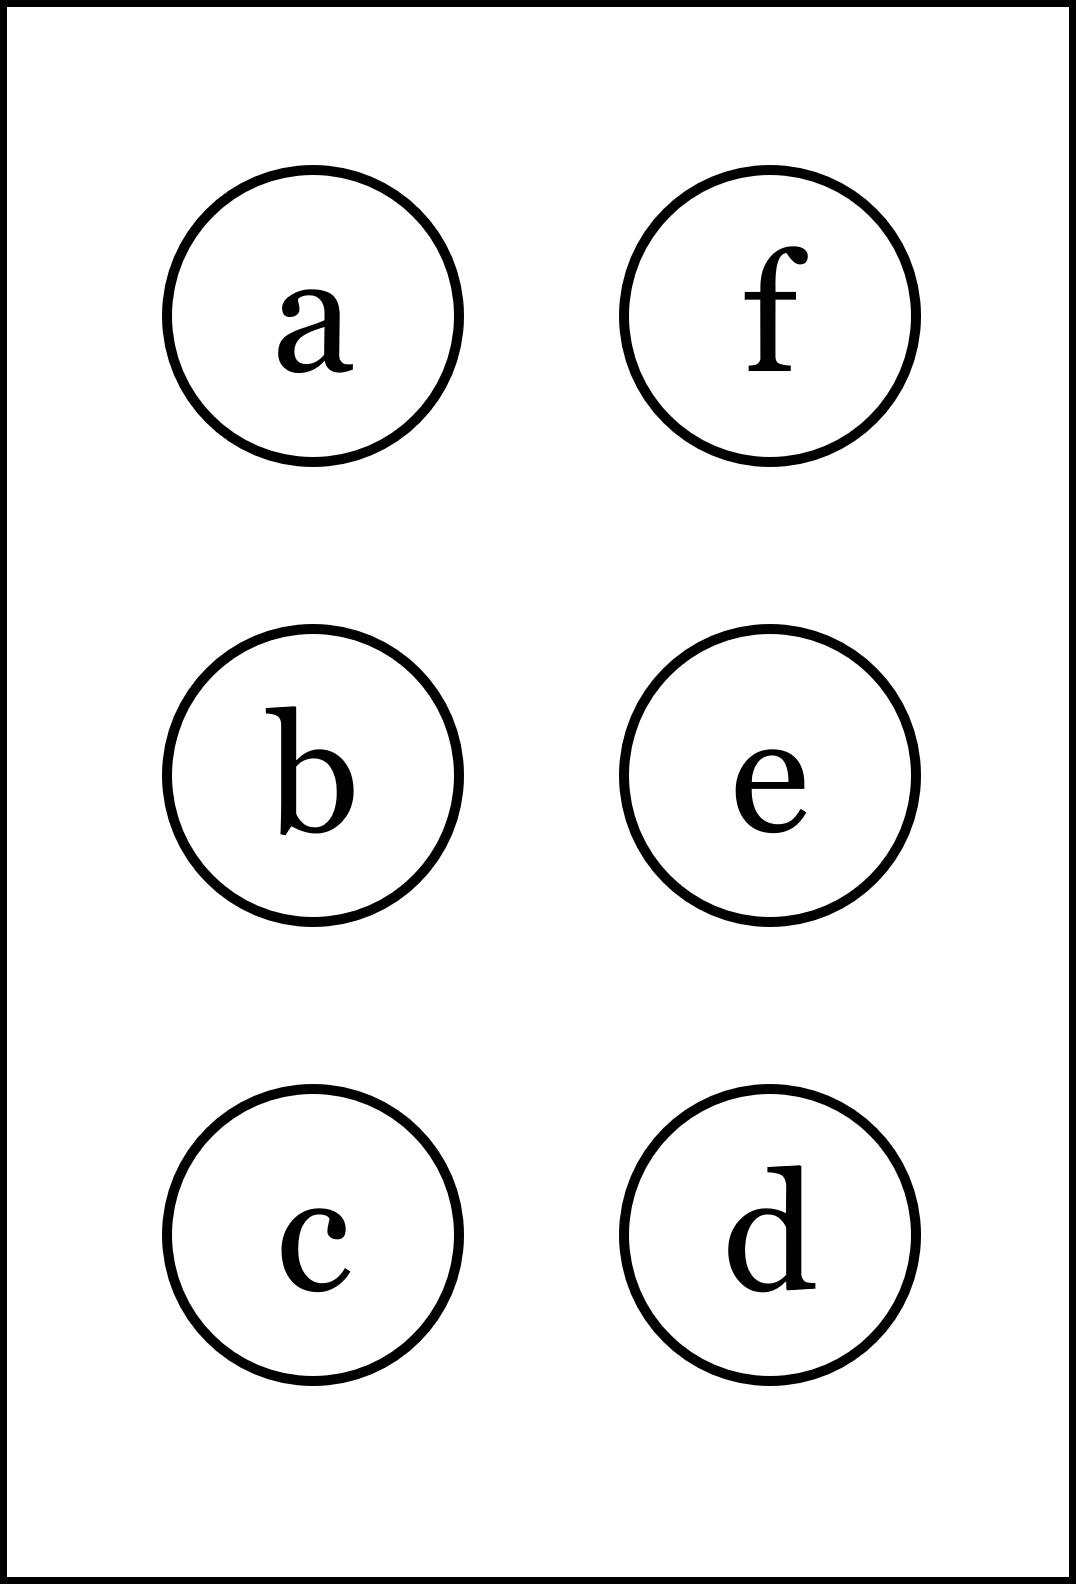
\includegraphics[height=40mm]{../images/braille.png}
{\small Písmeno Braillovej abecedy}
\end{center}
\end{minipage}
\end{center}
\end{minipage}
%
\end{tabular}
\newpage
\thispagestyle{empty}
\begin{tabular}{c:c}
\begin{minipage}[c][104.5mm][t]{0.5\linewidth}
\begin{center}
\vspace{7mm}
{\huge Závorky a zlomky, skupina \textit{Delta $\delta$} -\romannumeral1}\\[5mm]
\textit{Jméno:}\phantom{xxxxxxxxxxxxxxxxxxxxxxxxxxxxxxxxxxxxxxxxxxxxxxxxxxxxxxxxxxxxxxxxx}\\[5mm]
\begin{minipage}{0.95\linewidth}
\begin{center}
\textbf{Uprav výrazy (a) až (f)}. Pokud je výraz za otazníky roven výrazu pred otázniky, tak napravo obarvi príslušející kroužek. \textbf{Spolu odevzdejte výsledné slovo.}
\end{center}
\end{minipage}
\\[1mm]
\begin{minipage}{0.79\linewidth}
\begin{center}
\begin{varwidth}{\linewidth}
\begin{enumerate}
\normalsize
\item $3(-x-2)-2(4+3x)$\quad \dotfill\; ???\;\dotfill \quad $-9x-14$
\item $2(2-4x)(5x+1)-7(-2+9x)$\quad \dotfill\; ???\;\dotfill \quad $-40x^2+51x$
\item $(4x-1)^3-(2x+4)^2$\quad \dotfill\; ???\;\dotfill \quad $-64x^3+52x^2-4x-17$
\item $\cfrac{7x-6}{5}-2\cfrac{-2+7x}{5}$\quad \dotfill\; ???\;\dotfill \quad $\cfrac{-35x-10}{25}$
\item $\cfrac{\frac{3}{-2}-\frac{6}{x}}{\frac{1}{-2}+\frac{5}{-4}}$\quad \dotfill\; ???\;\dotfill \quad $\cfrac{26x+99}{28x}$
\item $\cfrac{(1-3x)^2-4}{(6x+3)\cdot\frac{-7}{x}}$\quad \dotfill\; ???\;\dotfill \quad $\cfrac{9x^3-6x^2-3x}{-42x-21}$
\end{enumerate}
\end{varwidth}
\end{center}
\end{minipage}
\begin{minipage}{0.20\linewidth}
\begin{center}
{\Huge\bfseries 1.} \\[2mm]
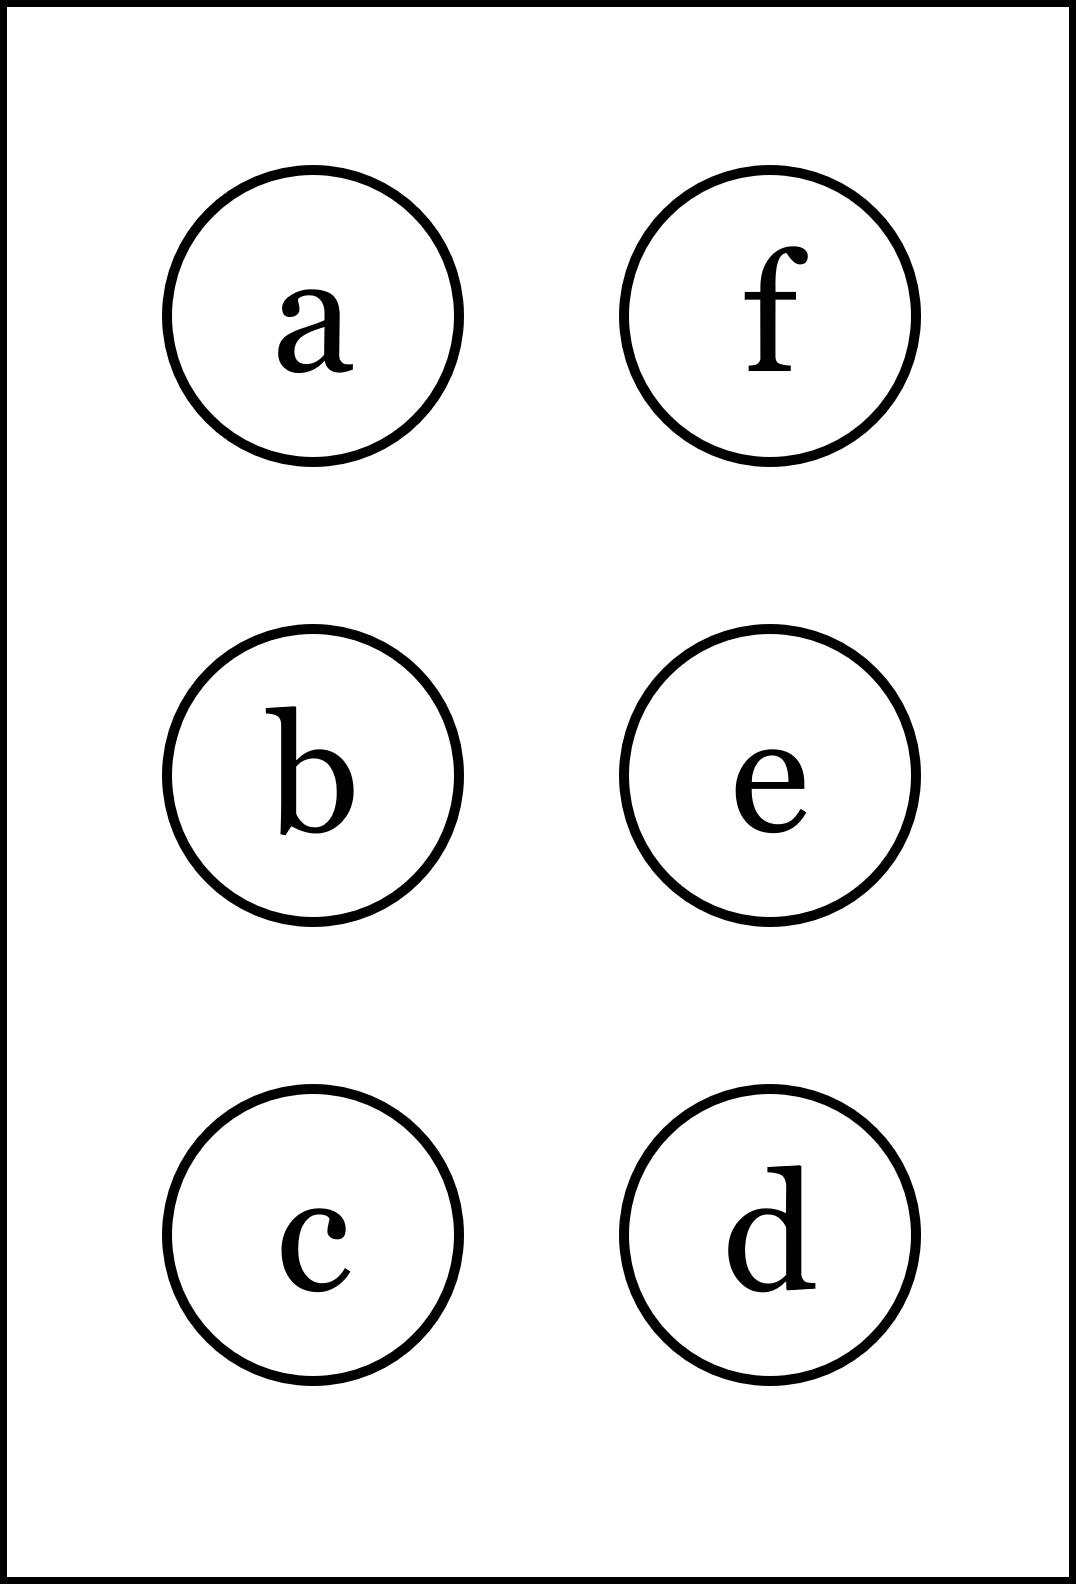
\includegraphics[height=40mm]{../images/braille.png}
{\small Písmeno Braillovej abecedy}
\end{center}
\end{minipage}
\end{center}
\end{minipage}
&
\begin{minipage}[c][104.5mm][t]{0.5\linewidth}
\begin{center}
\vspace{7mm}
{\huge Závorky a zlomky, skupina \textit{Delta $\delta$} -\romannumeral2}\\[5mm]
\textit{Jméno:}\phantom{xxxxxxxxxxxxxxxxxxxxxxxxxxxxxxxxxxxxxxxxxxxxxxxxxxxxxxxxxxxxxxxxx}\\[5mm]
\begin{minipage}{0.95\linewidth}
\begin{center}
\textbf{Uprav výrazy (a) až (f)}. Pokud je výraz za otazníky roven výrazu pred otázniky, tak napravo obarvi príslušející kroužek. \textbf{Spolu odevzdejte výsledné slovo.}
\end{center}
\end{minipage}
\\[1mm]
\begin{minipage}{0.79\linewidth}
\begin{center}
\begin{varwidth}{\linewidth}
\begin{enumerate}
\normalsize
\item $8(7x-1)+1(3+x)$\quad \dotfill\; ???\;\dotfill \quad $57x+5$
\item $-3(5+x)(-3x+6)-2(6-3x)$\quad \dotfill\; ???\;\dotfill \quad $9x^2-33x-102$
\item $(4x+1)^3-(-2x+6)^2$\quad \dotfill\; ???\;\dotfill \quad $64x^3+44x^2+36x-35$
\item $\cfrac{2x+3}{-2}-2\cfrac{-1+3x}{-5}$\quad \dotfill\; ???\;\dotfill \quad $\cfrac{2x-19}{-10}$
\item $\cfrac{\frac{-3}{-2}-\frac{-4}{x}}{\frac{1}{2}+\frac{-1}{-2}}$\quad \dotfill\; ???\;\dotfill \quad $\cfrac{10x+35}{8x}$
\item $\cfrac{(-2+x)^2+2}{(4x-7)\cdot\frac{2}{x}}$\quad \dotfill\; ???\;\dotfill \quad $\cfrac{x^3-4x^2+6x}{8x-14}$
\end{enumerate}
\end{varwidth}
\end{center}
\end{minipage}
\begin{minipage}{0.20\linewidth}
\begin{center}
{\Huge\bfseries 2.} \\[2mm]
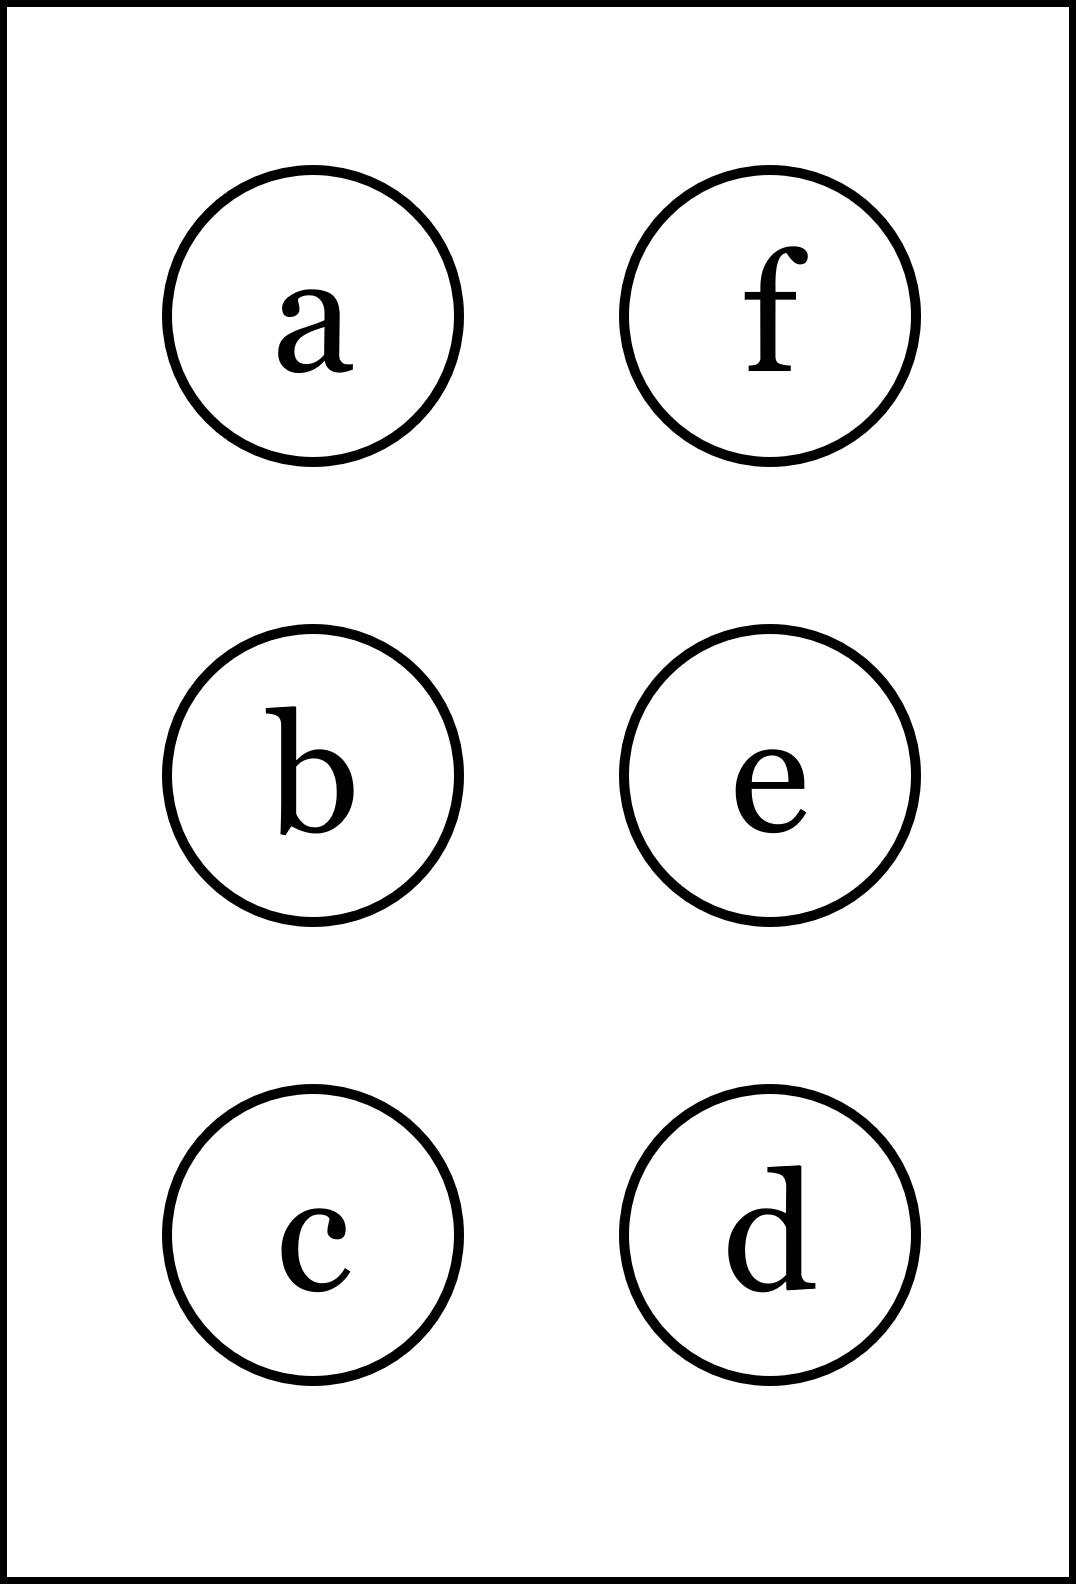
\includegraphics[height=40mm]{../images/braille.png}
{\small Písmeno Braillovej abecedy}
\end{center}
\end{minipage}
\end{center}
\end{minipage}
\\ \hdashline
\begin{minipage}[c][104.5mm][t]{0.5\linewidth}
\begin{center}
\vspace{7mm}
{\huge Závorky a zlomky, skupina \textit{Delta $\delta$} -\romannumeral3}\\[5mm]
\textit{Jméno:}\phantom{xxxxxxxxxxxxxxxxxxxxxxxxxxxxxxxxxxxxxxxxxxxxxxxxxxxxxxxxxxxxxxxxx}\\[5mm]
\begin{minipage}{0.95\linewidth}
\begin{center}
\textbf{Uprav výrazy (a) až (f)}. Pokud je výraz za otazníky roven výrazu pred otázniky, tak napravo obarvi príslušející kroužek. \textbf{Spolu odevzdejte výsledné slovo.}
\end{center}
\end{minipage}
\\[1mm]
\begin{minipage}{0.79\linewidth}
\begin{center}
\begin{varwidth}{\linewidth}
\begin{enumerate}
\normalsize
\item $2(-x-2)+2(4+4x)$\quad \dotfill\; ???\;\dotfill \quad $6x+4$
\item $-4(2+3x)(7x-6)-1(6+6x)$\quad \dotfill\; ???\;\dotfill \quad $-84x^2-10x-42$
\item $(-4x-1)^3-(3x-5)^2$\quad \dotfill\; ???\;\dotfill \quad $-64x^3-57x^2+18x-26$
\item $\cfrac{5x-3}{7}+2\cfrac{4+2x}{2}$\quad \dotfill\; ???\;\dotfill \quad $\cfrac{38x+50}{-14}$
\item $\cfrac{\frac{7}{-2}-\frac{4}{x}}{\frac{1}{4}+\frac{-1}{3}}$\quad \dotfill\; ???\;\dotfill \quad $\cfrac{84x+96}{2x}$
\item $\cfrac{(-4-4x)^2+8}{(-5x-4)\cdot\frac{2}{x}}$\quad \dotfill\; ???\;\dotfill \quad $\cfrac{16x^3+32x^2+24x}{-10x-8}$
\end{enumerate}
\end{varwidth}
\end{center}
\end{minipage}
\begin{minipage}{0.20\linewidth}
\begin{center}
{\Huge\bfseries 3.} \\[2mm]
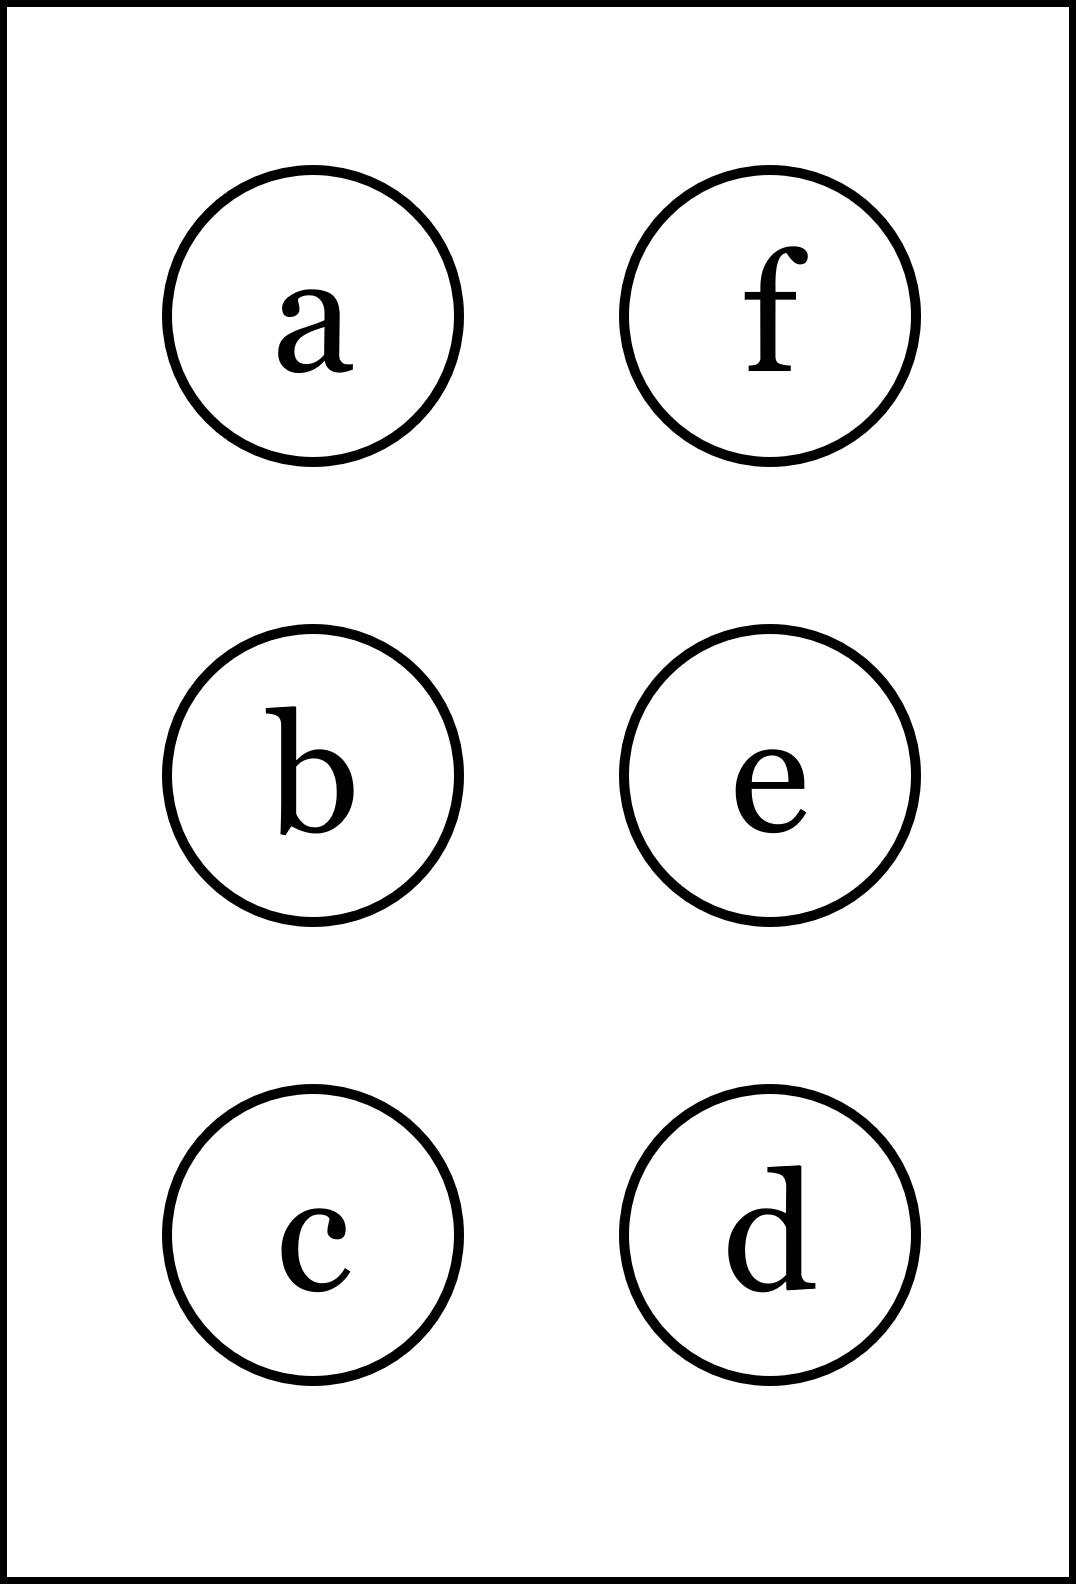
\includegraphics[height=40mm]{../images/braille.png}
{\small Písmeno Braillovej abecedy}
\end{center}
\end{minipage}
\end{center}
\end{minipage}
&
\begin{minipage}[c][104.5mm][t]{0.5\linewidth}
\begin{center}
\vspace{7mm}
{\huge Závorky a zlomky, skupina \textit{Delta $\delta$} -\romannumeral4}\\[5mm]
\textit{Jméno:}\phantom{xxxxxxxxxxxxxxxxxxxxxxxxxxxxxxxxxxxxxxxxxxxxxxxxxxxxxxxxxxxxxxxxx}\\[5mm]
\begin{minipage}{0.95\linewidth}
\begin{center}
\textbf{Uprav výrazy (a) až (f)}. Pokud je výraz za otazníky roven výrazu pred otázniky, tak napravo obarvi príslušející kroužek. \textbf{Spolu odevzdejte výsledné slovo.}
\end{center}
\end{minipage}
\\[1mm]
\begin{minipage}{0.79\linewidth}
\begin{center}
\begin{varwidth}{\linewidth}
\begin{enumerate}
\normalsize
\item $-6(5x-1)-6(3+x)$\quad \dotfill\; ???\;\dotfill \quad $-36x-12$
\item $-4(-5-2x)(-x-2)-2(2-3x)$\quad \dotfill\; ???\;\dotfill \quad $-8x^2+30x+44$
\item $(-2x+4)^3-(-7x-5)^2$\quad \dotfill\; ???\;\dotfill \quad $8x^3+x^2-166x+39$
\item $\cfrac{-2x-4}{-4}-3\cfrac{3-x}{-9}$\quad \dotfill\; ???\;\dotfill \quad $\cfrac{-6x+72}{-36}$
\item $\cfrac{\frac{-3}{4}-\frac{4}{x}}{\frac{1}{1}+\frac{-3}{-5}}$\quad \dotfill\; ???\;\dotfill \quad $\cfrac{18x+79}{-32x}$
\item $\cfrac{(1+x)^2+3}{(-x-7)\cdot\frac{-2}{x}}$\quad \dotfill\; ???\;\dotfill \quad $\cfrac{x^3+2x^2-4x}{-2x+14}$
\end{enumerate}
\end{varwidth}
\end{center}
\end{minipage}
\begin{minipage}{0.20\linewidth}
\begin{center}
{\Huge\bfseries 4.} \\[2mm]
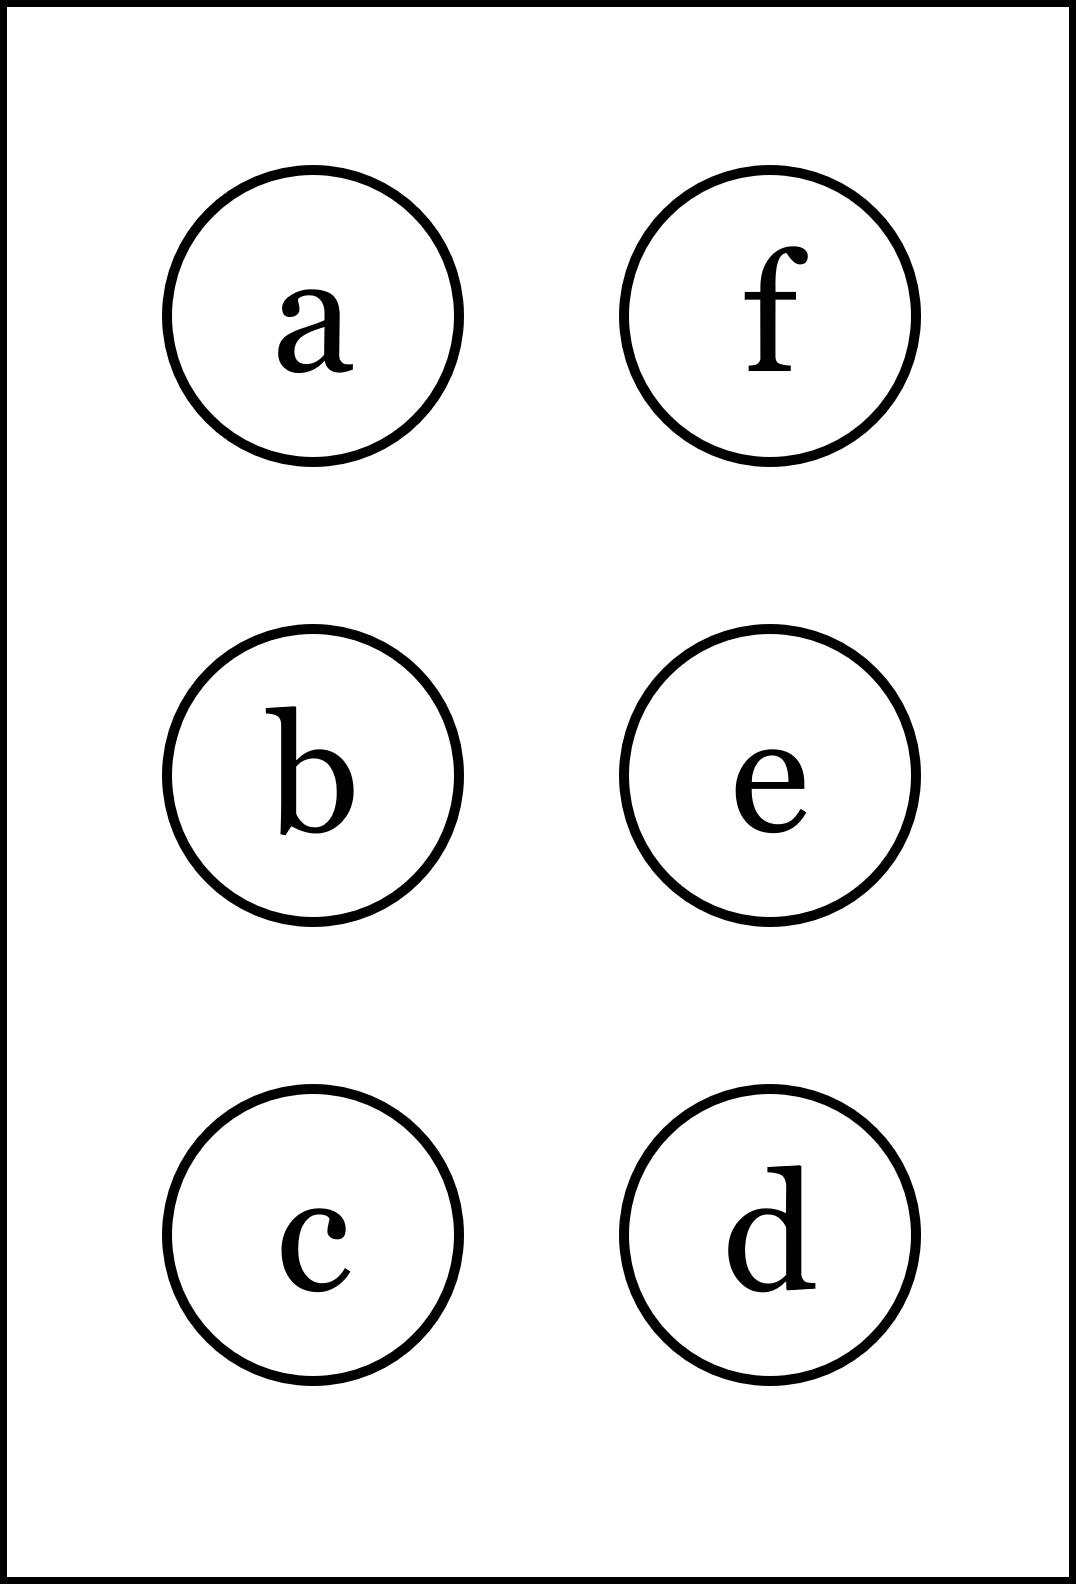
\includegraphics[height=40mm]{../images/braille.png}
{\small Písmeno Braillovej abecedy}
\end{center}
\end{minipage}
\end{center}
\end{minipage}
%
\end{tabular}
\newpage
\thispagestyle{empty}
\begin{tabular}{c:c}
\begin{minipage}[c][104.5mm][t]{0.5\linewidth}
\begin{center}
\vspace{7mm}
{\huge Závorky a zlomky, skupina \textit{Epsilon $\epsilon$} -\romannumeral1}\\[5mm]
\textit{Jméno:}\phantom{xxxxxxxxxxxxxxxxxxxxxxxxxxxxxxxxxxxxxxxxxxxxxxxxxxxxxxxxxxxxxxxxx}\\[5mm]
\begin{minipage}{0.95\linewidth}
\begin{center}
\textbf{Uprav výrazy (a) až (f)}. Pokud je výraz za otazníky roven výrazu pred otázniky, tak napravo obarvi príslušející kroužek. \textbf{Spolu odevzdejte výsledné slovo.}
\end{center}
\end{minipage}
\\[1mm]
\begin{minipage}{0.79\linewidth}
\begin{center}
\begin{varwidth}{\linewidth}
\begin{enumerate}
\normalsize
\item $2(-3x+1)-6(-8-4x)$\quad \dotfill\; ???\;\dotfill \quad $18x$
\item $9(-4+7x)(x+1)+5(-4-8x)$\quad \dotfill\; ???\;\dotfill \quad $63x^2+13x$
\item $(x-1)^3-(5x+3)^2$\quad \dotfill\; ???\;\dotfill \quad $x^3-28x^2-27x-10$
\item $\cfrac{3x-7}{5}+2\cfrac{-8-3x}{-2}$\quad \dotfill\; ???\;\dotfill \quad $\cfrac{-36x-66}{-10}$
\item $\cfrac{\frac{-1}{8}-\frac{1}{x}}{\frac{1}{2}+\frac{-3}{-1}}$\quad \dotfill\; ???\;\dotfill \quad $\cfrac{5x+17}{-56x}$
\item $\cfrac{(-7+9x)^2-4}{(-2x+9)\cdot\frac{2}{x}}$\quad \dotfill\; ???\;\dotfill \quad $\cfrac{81x^3-126x^2+45x}{-4x+18}$
\end{enumerate}
\end{varwidth}
\end{center}
\end{minipage}
\begin{minipage}{0.20\linewidth}
\begin{center}
{\Huge\bfseries 1.} \\[2mm]
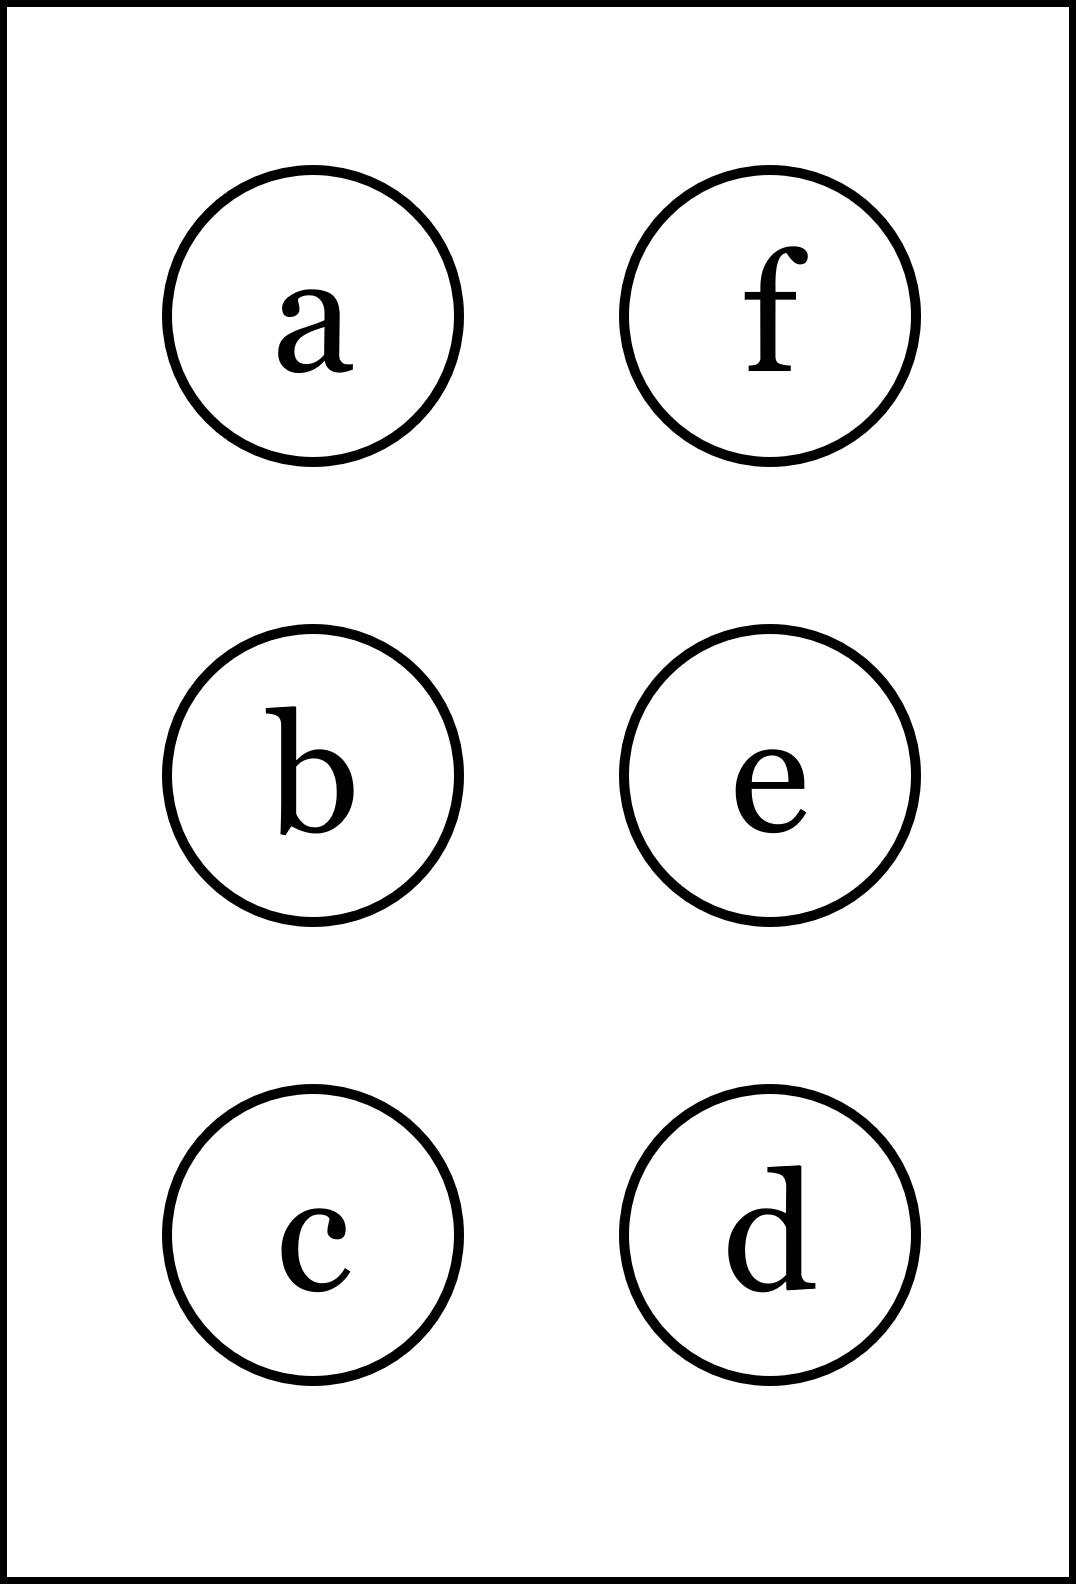
\includegraphics[height=40mm]{../images/braille.png}
{\small Písmeno Braillovej abecedy}
\end{center}
\end{minipage}
\end{center}
\end{minipage}
&
\begin{minipage}[c][104.5mm][t]{0.5\linewidth}
\begin{center}
\vspace{7mm}
{\huge Závorky a zlomky, skupina \textit{Epsilon $\epsilon$} -\romannumeral2}\\[5mm]
\textit{Jméno:}\phantom{xxxxxxxxxxxxxxxxxxxxxxxxxxxxxxxxxxxxxxxxxxxxxxxxxxxxxxxxxxxxxxxxx}\\[5mm]
\begin{minipage}{0.95\linewidth}
\begin{center}
\textbf{Uprav výrazy (a) až (f)}. Pokud je výraz za otazníky roven výrazu pred otázniky, tak napravo obarvi príslušející kroužek. \textbf{Spolu odevzdejte výsledné slovo.}
\end{center}
\end{minipage}
\\[1mm]
\begin{minipage}{0.79\linewidth}
\begin{center}
\begin{varwidth}{\linewidth}
\begin{enumerate}
\normalsize
\item $-2(x-2)-6(-5-x)$\quad \dotfill\; ???\;\dotfill \quad $4x+34$
\item $-2(-2+5x)(2x+4)-3(2+6x)$\quad \dotfill\; ???\;\dotfill \quad $-20x^2-50x+10$
\item $(3x-4)^3-(-6x-7)^2$\quad \dotfill\; ???\;\dotfill \quad $27x^3-144x^2+60x-113$
\item $\cfrac{-6x+2}{3}+6\cfrac{1+x}{-3}$\quad \dotfill\; ???\;\dotfill \quad $\cfrac{12}{9}$
\item $\cfrac{\frac{-6}{4}-\frac{-1}{x}}{\frac{1}{1}+\frac{1}{7}}$\quad \dotfill\; ???\;\dotfill \quad $\cfrac{-39x+31}{32x}$
\item $\cfrac{(-1-2x)^2-6}{(7x-4)\cdot\frac{5}{x}}$\quad \dotfill\; ???\;\dotfill \quad $\cfrac{4x^3+4x^2-5x}{35x-20}$
\end{enumerate}
\end{varwidth}
\end{center}
\end{minipage}
\begin{minipage}{0.20\linewidth}
\begin{center}
{\Huge\bfseries 2.} \\[2mm]
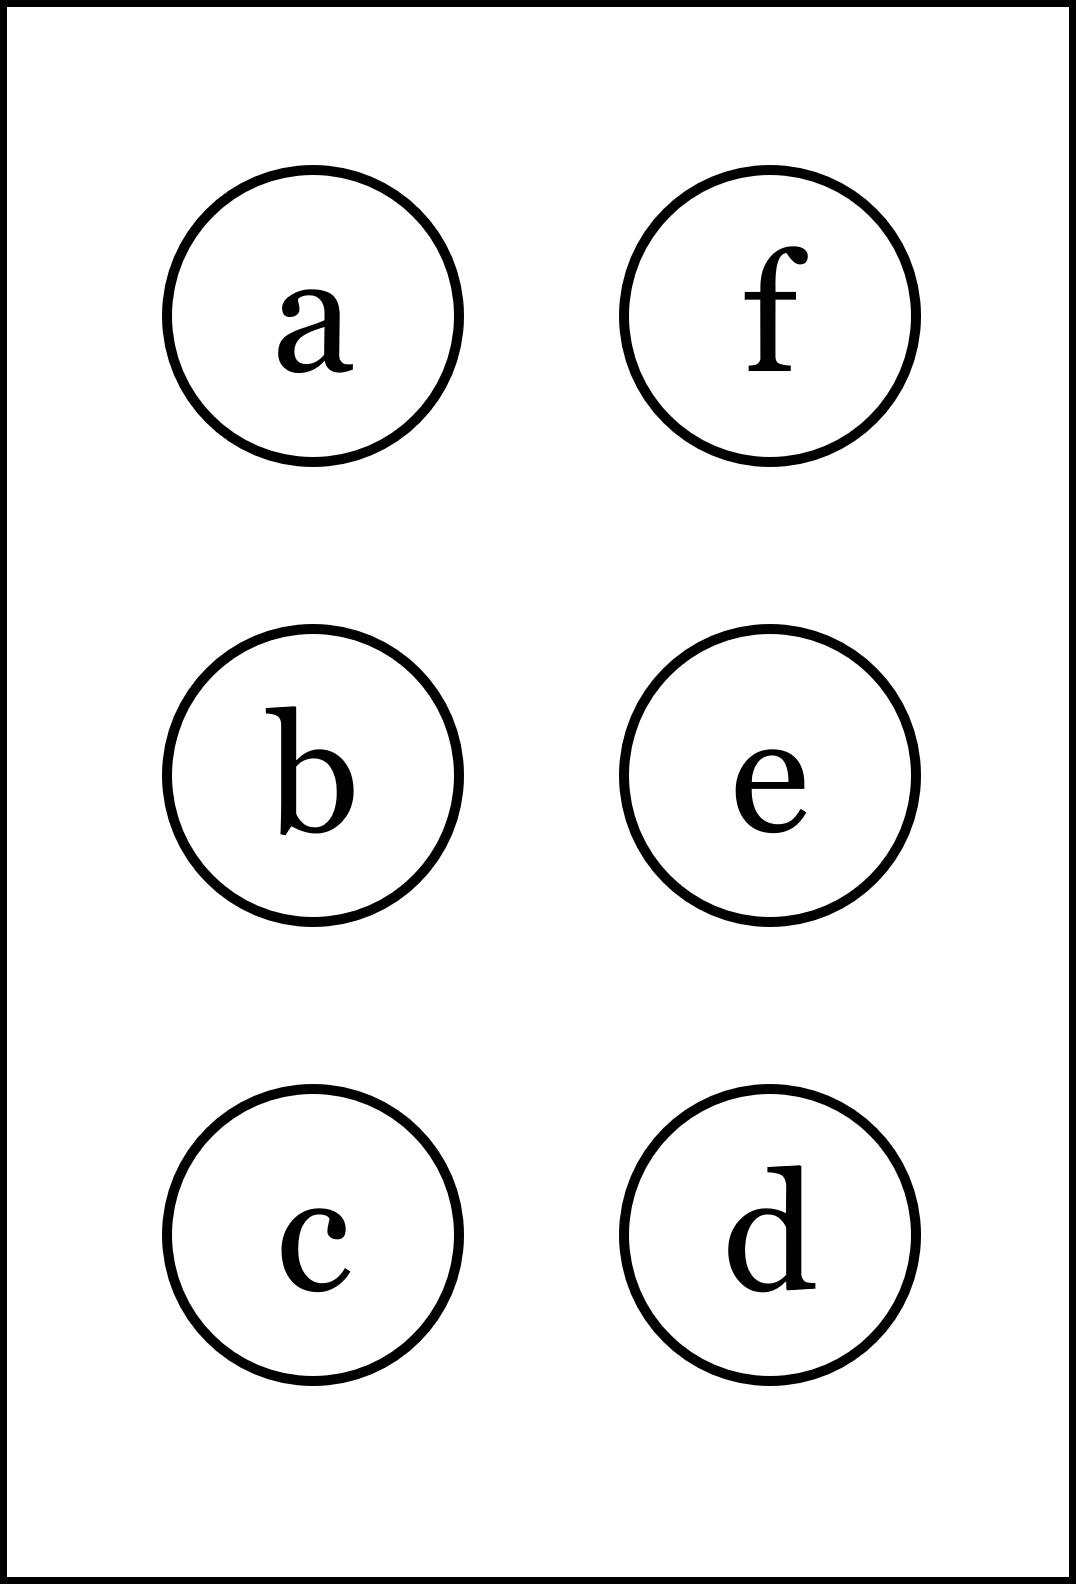
\includegraphics[height=40mm]{../images/braille.png}
{\small Písmeno Braillovej abecedy}
\end{center}
\end{minipage}
\end{center}
\end{minipage}
\\ \hdashline
\begin{minipage}[c][104.5mm][t]{0.5\linewidth}
\begin{center}
\vspace{7mm}
{\huge Závorky a zlomky, skupina \textit{Epsilon $\epsilon$} -\romannumeral3}\\[5mm]
\textit{Jméno:}\phantom{xxxxxxxxxxxxxxxxxxxxxxxxxxxxxxxxxxxxxxxxxxxxxxxxxxxxxxxxxxxxxxxxx}\\[5mm]
\begin{minipage}{0.95\linewidth}
\begin{center}
\textbf{Uprav výrazy (a) až (f)}. Pokud je výraz za otazníky roven výrazu pred otázniky, tak napravo obarvi príslušející kroužek. \textbf{Spolu odevzdejte výsledné slovo.}
\end{center}
\end{minipage}
\\[1mm]
\begin{minipage}{0.79\linewidth}
\begin{center}
\begin{varwidth}{\linewidth}
\begin{enumerate}
\normalsize
\item $7(-x+1)-5(-1+4x)$\quad \dotfill\; ???\;\dotfill \quad $-27x+12$
\item $-5(-2+2x)(6x+1)-3(3+3x)$\quad \dotfill\; ???\;\dotfill \quad $-60x^2-41x-1$
\item $(-3x+2)^3-(-2x+3)^2$\quad \dotfill\; ???\;\dotfill \quad $27x^3+50x^2-1$
\item $\cfrac{-2x-5}{8}-2\cfrac{3-x}{8}$\quad \dotfill\; ???\;\dotfill \quad $\cfrac{-88}{-64}$
\item $\cfrac{\frac{-3}{-4}-\frac{1}{x}}{\frac{1}{-1}+\frac{-4}{-8}}$\quad \dotfill\; ???\;\dotfill \quad $\cfrac{-25x+31}{16x}$
\item $\cfrac{(3+3x)^2+6}{(-6x-2)\cdot\frac{-4}{x}}$\quad \dotfill\; ???\;\dotfill \quad $\cfrac{9x^3+18x^2-15x}{-24x+8}$
\end{enumerate}
\end{varwidth}
\end{center}
\end{minipage}
\begin{minipage}{0.20\linewidth}
\begin{center}
{\Huge\bfseries 3.} \\[2mm]
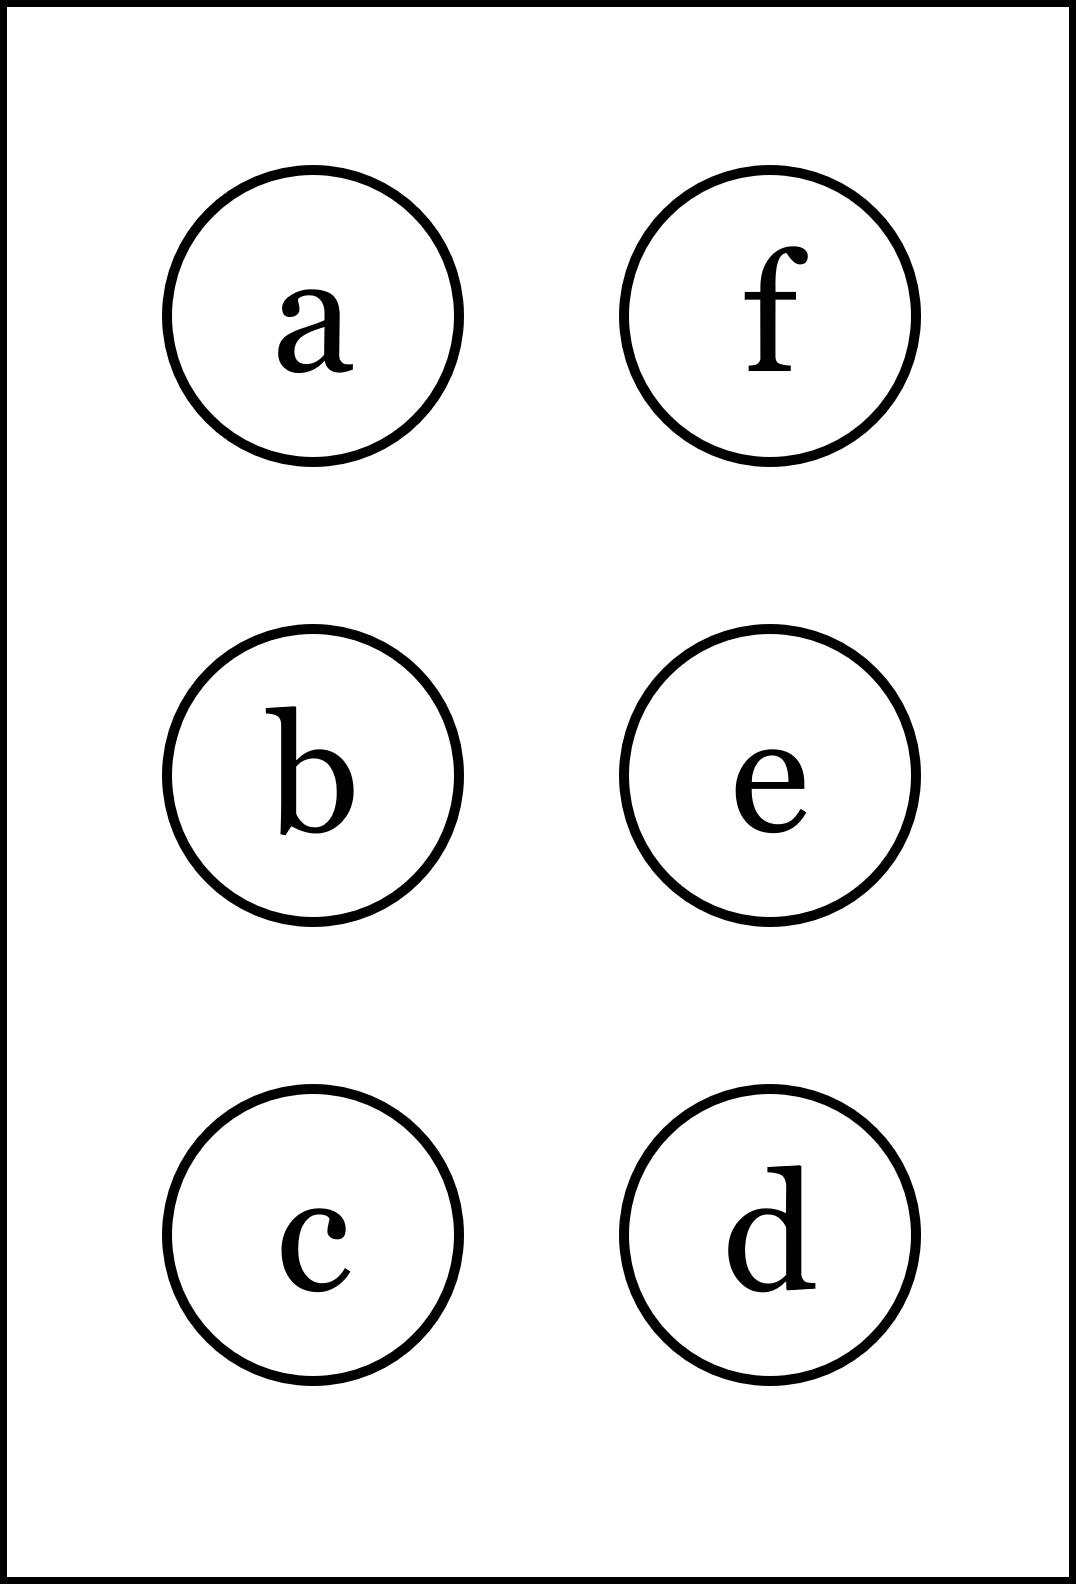
\includegraphics[height=40mm]{../images/braille.png}
{\small Písmeno Braillovej abecedy}
\end{center}
\end{minipage}
\end{center}
\end{minipage}
&
\begin{minipage}[c][104.5mm][t]{0.5\linewidth}
\begin{center}
\vspace{7mm}
{\huge Závorky a zlomky, skupina \textit{Epsilon $\epsilon$} -\romannumeral4}\\[5mm]
\textit{Jméno:}\phantom{xxxxxxxxxxxxxxxxxxxxxxxxxxxxxxxxxxxxxxxxxxxxxxxxxxxxxxxxxxxxxxxxx}\\[5mm]
\begin{minipage}{0.95\linewidth}
\begin{center}
\textbf{Uprav výrazy (a) až (f)}. Pokud je výraz za otazníky roven výrazu pred otázniky, tak napravo obarvi príslušející kroužek. \textbf{Spolu odevzdejte výsledné slovo.}
\end{center}
\end{minipage}
\\[1mm]
\begin{minipage}{0.79\linewidth}
\begin{center}
\begin{varwidth}{\linewidth}
\begin{enumerate}
\normalsize
\item $2(-3x-8)-4(6-3x)$\quad \dotfill\; ???\;\dotfill \quad $6x-40$
\item $2(-7+9x)(-3x+4)-9(-2+2x)$\quad \dotfill\; ???\;\dotfill \quad $-54x^2+96x-38$
\item $(-x-1)^3-(-2x+6)^2$\quad \dotfill\; ???\;\dotfill \quad $-x^3-7x^2+21x-37$
\item $\cfrac{-2x-1}{4}-4\cfrac{-1+6x}{3}$\quad \dotfill\; ???\;\dotfill \quad $\cfrac{102x+13}{-12}$
\item $\cfrac{\frac{-2}{3}-\frac{-2}{x}}{\frac{1}{4}+\frac{2}{-1}}$\quad \dotfill\; ???\;\dotfill \quad $\cfrac{11x-26}{21x}$
\item $\cfrac{(6-9x)^2+5}{(6x-9)\cdot\frac{-6}{x}}$\quad \dotfill\; ???\;\dotfill \quad $\cfrac{81x^3-108x^2-41x}{36x+54}$
\end{enumerate}
\end{varwidth}
\end{center}
\end{minipage}
\begin{minipage}{0.20\linewidth}
\begin{center}
{\Huge\bfseries 4.} \\[2mm]
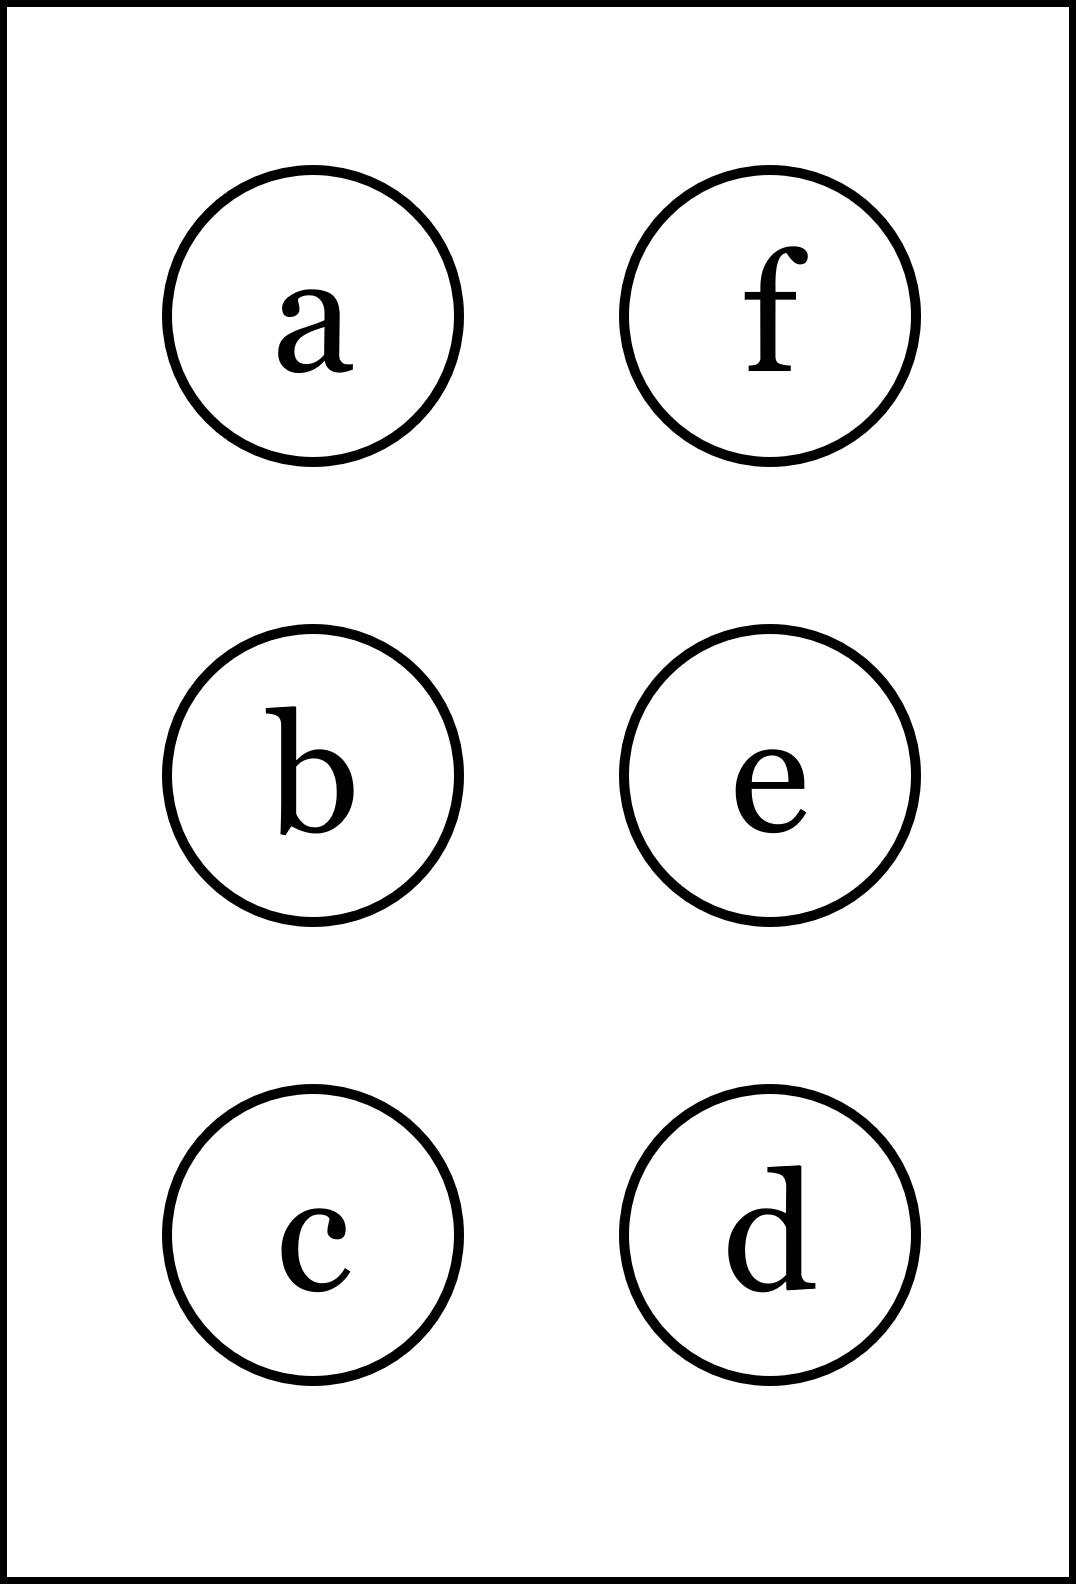
\includegraphics[height=40mm]{../images/braille.png}
{\small Písmeno Braillovej abecedy}
\end{center}
\end{minipage}
\end{center}
\end{minipage}
%
\end{tabular}
\newpage
\thispagestyle{empty}
\begin{tabular}{c:c}
\begin{minipage}[c][104.5mm][t]{0.5\linewidth}
\begin{center}
\vspace{7mm}
{\huge Závorky a zlomky, skupina \textit{Zeta $\zeta$} -\romannumeral1}\\[5mm]
\textit{Jméno:}\phantom{xxxxxxxxxxxxxxxxxxxxxxxxxxxxxxxxxxxxxxxxxxxxxxxxxxxxxxxxxxxxxxxxx}\\[5mm]
\begin{minipage}{0.95\linewidth}
\begin{center}
\textbf{Uprav výrazy (a) až (f)}. Pokud je výraz za otazníky roven výrazu pred otázniky, tak napravo obarvi príslušející kroužek. \textbf{Spolu odevzdejte výsledné slovo.}
\end{center}
\end{minipage}
\\[1mm]
\begin{minipage}{0.79\linewidth}
\begin{center}
\begin{varwidth}{\linewidth}
\begin{enumerate}
\normalsize
\item $9(x+8)-4(-8+5x)$\quad \dotfill\; ???\;\dotfill \quad $-11x$
\item $-5(-1+2x)(-8x+1)+5(-8-7x)$\quad \dotfill\; ???\;\dotfill \quad $80x^2-85x-35$
\item $(-x-1)^3-(2x-6)^2$\quad \dotfill\; ???\;\dotfill \quad $x^3-7x^2+21x-37$
\item $\cfrac{-4x+3}{2}-2\cfrac{8-4x}{-5}$\quad \dotfill\; ???\;\dotfill \quad $\cfrac{36x-47}{10}$
\item $\cfrac{\frac{-5}{4}-\frac{6}{x}}{\frac{1}{-3}+\frac{6}{1}}$\quad \dotfill\; ???\;\dotfill \quad $\cfrac{13x+73}{-68x}$
\item $\cfrac{(-7-8x)^2-3}{(2x-4)\cdot\frac{-2}{x}}$\quad \dotfill\; ???\;\dotfill \quad $\cfrac{64x^3+112x^2+46x}{-4x+8}$
\end{enumerate}
\end{varwidth}
\end{center}
\end{minipage}
\begin{minipage}{0.20\linewidth}
\begin{center}
{\Huge\bfseries 1.} \\[2mm]
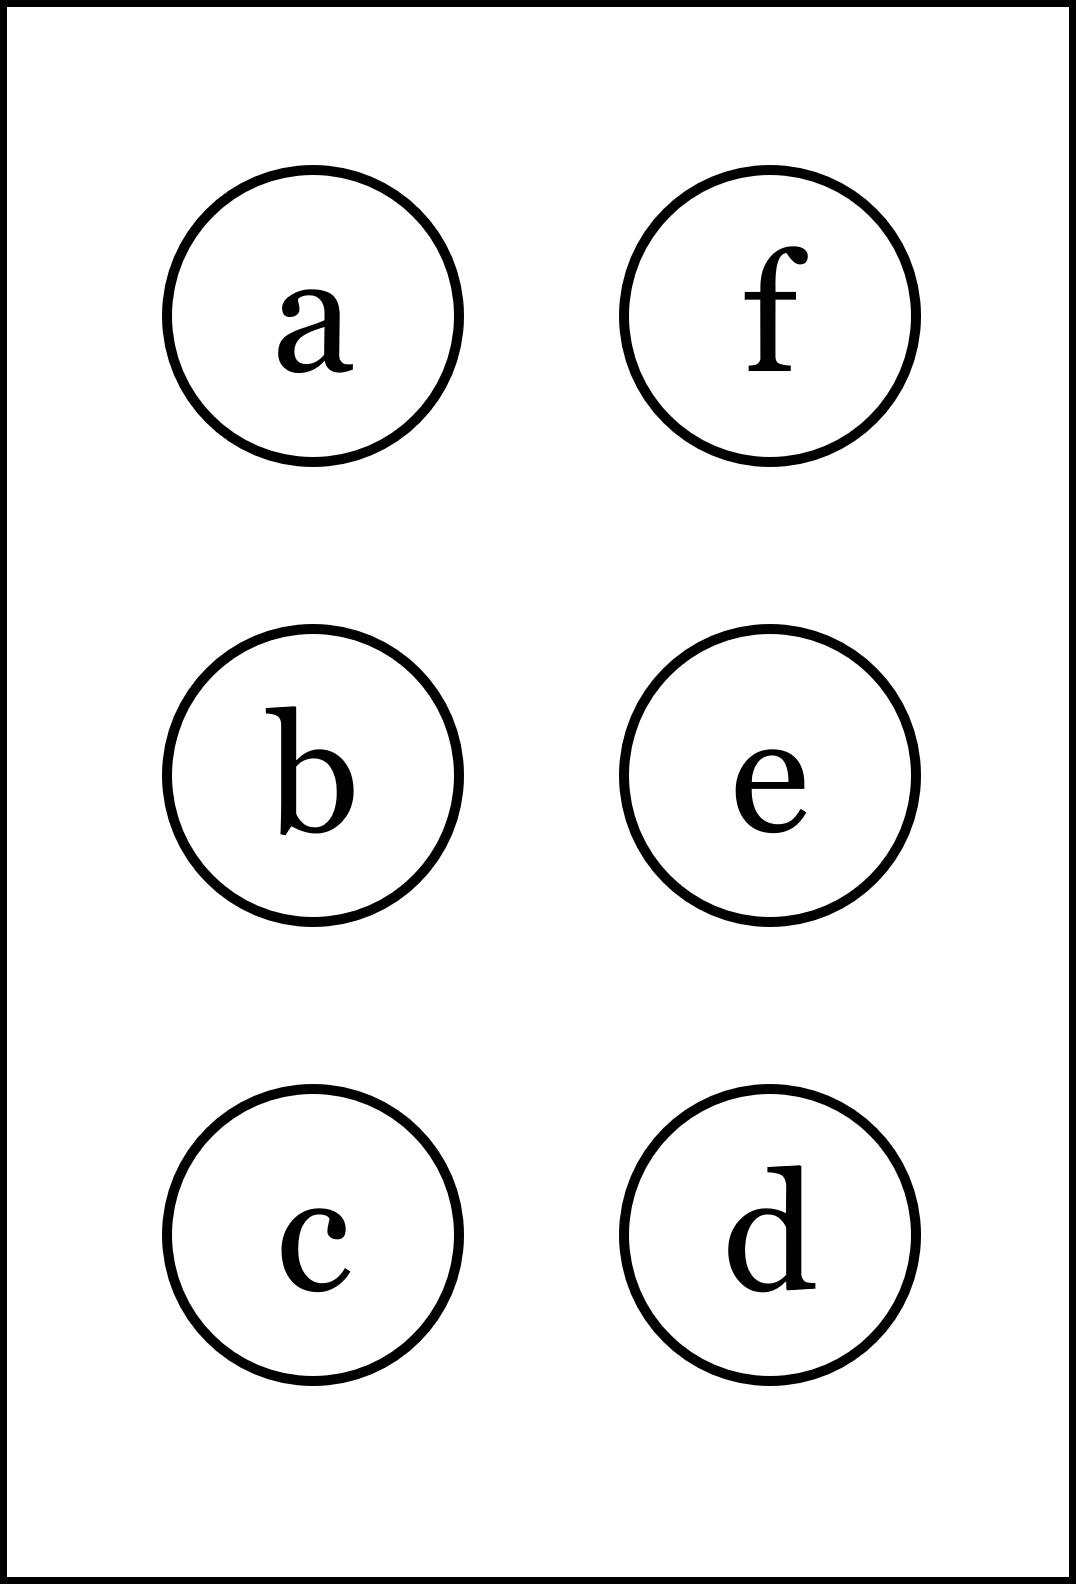
\includegraphics[height=40mm]{../images/braille.png}
{\small Písmeno Braillovej abecedy}
\end{center}
\end{minipage}
\end{center}
\end{minipage}
&
\begin{minipage}[c][104.5mm][t]{0.5\linewidth}
\begin{center}
\vspace{7mm}
{\huge Závorky a zlomky, skupina \textit{Zeta $\zeta$} -\romannumeral2}\\[5mm]
\textit{Jméno:}\phantom{xxxxxxxxxxxxxxxxxxxxxxxxxxxxxxxxxxxxxxxxxxxxxxxxxxxxxxxxxxxxxxxxx}\\[5mm]
\begin{minipage}{0.95\linewidth}
\begin{center}
\textbf{Uprav výrazy (a) až (f)}. Pokud je výraz za otazníky roven výrazu pred otázniky, tak napravo obarvi príslušející kroužek. \textbf{Spolu odevzdejte výsledné slovo.}
\end{center}
\end{minipage}
\\[1mm]
\begin{minipage}{0.79\linewidth}
\begin{center}
\begin{varwidth}{\linewidth}
\begin{enumerate}
\normalsize
\item $-6(-4x-3)+2(-6-5x)$\quad \dotfill\; ???\;\dotfill \quad $14x+6$
\item $-2(-3-2x)(8x-1)-6(5-9x)$\quad \dotfill\; ???\;\dotfill \quad $32x^2+98x-36$
\item $(4x-2)^3-(-x+1)^2$\quad \dotfill\; ???\;\dotfill \quad $-64x^3+97x^2+50x-9$
\item $\cfrac{4x+6}{5}+2\cfrac{-4-6x}{-5}$\quad \dotfill\; ???\;\dotfill \quad $\cfrac{-70}{25}$
\item $\cfrac{\frac{1}{3}-\frac{1}{x}}{\frac{1}{-2}+\frac{5}{-3}}$\quad \dotfill\; ???\;\dotfill \quad $\cfrac{6x-18}{-39x}$
\item $\cfrac{(-1-x)^2+7}{(x-6)\cdot\frac{3}{x}}$\quad \dotfill\; ???\;\dotfill \quad $\cfrac{x^3+2x^2+8x}{3x-18}$
\end{enumerate}
\end{varwidth}
\end{center}
\end{minipage}
\begin{minipage}{0.20\linewidth}
\begin{center}
{\Huge\bfseries 2.} \\[2mm]
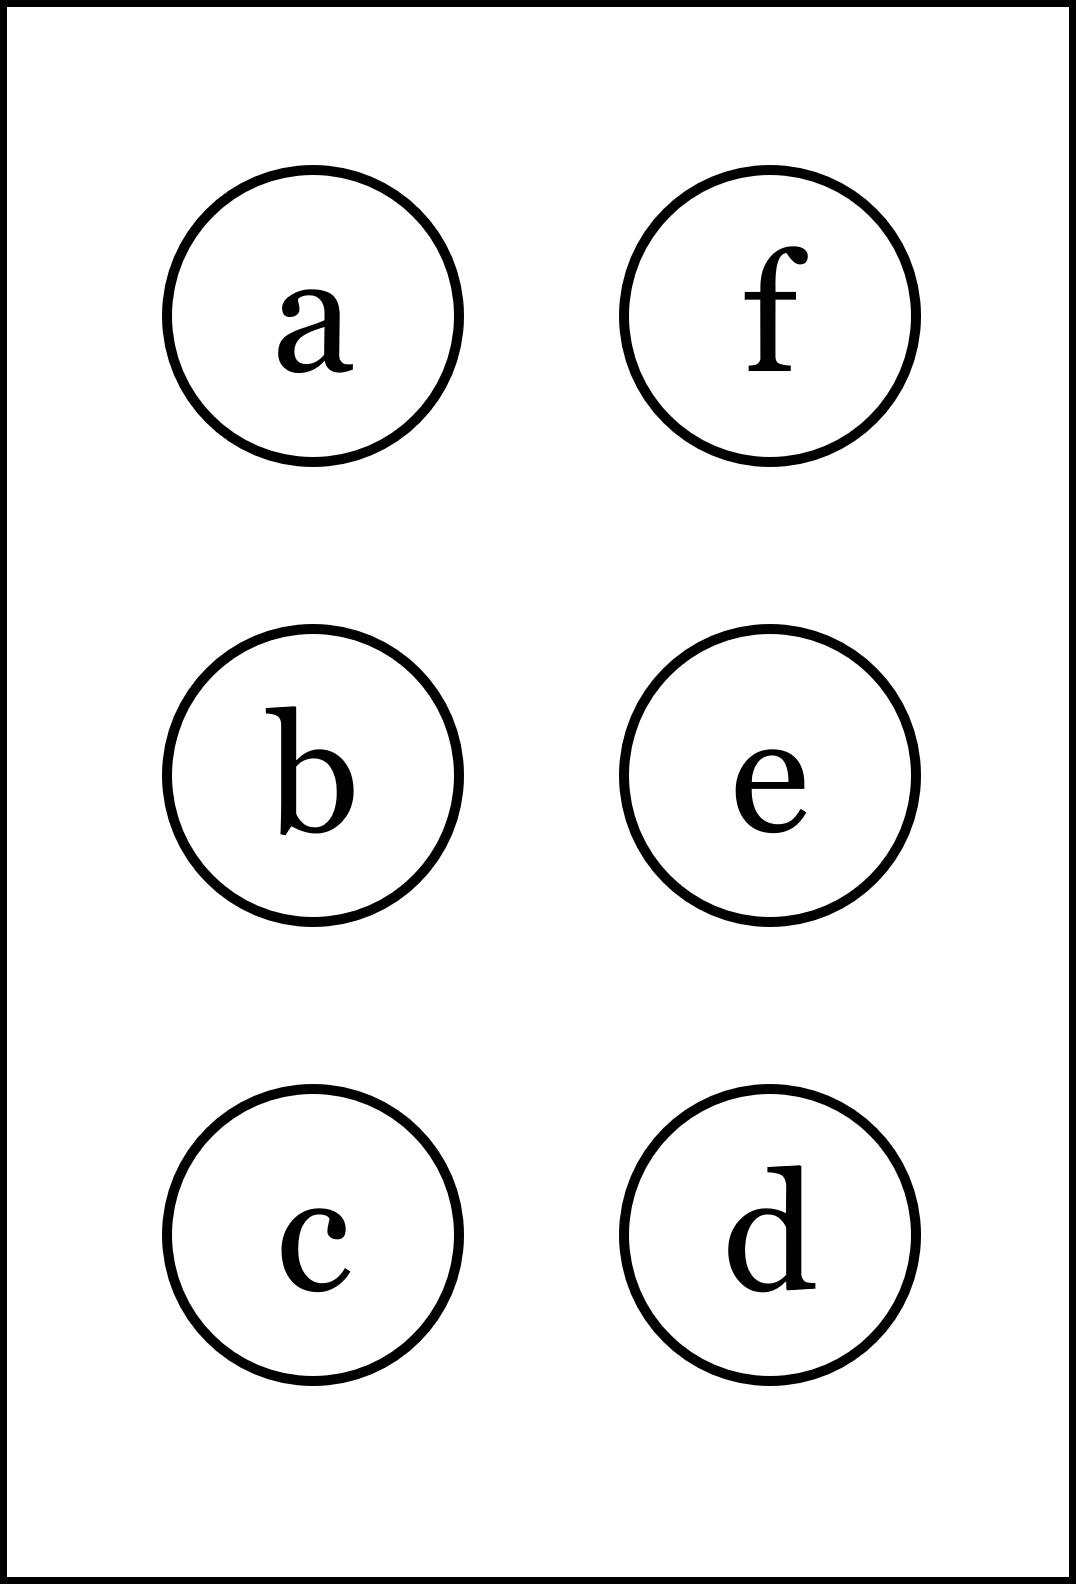
\includegraphics[height=40mm]{../images/braille.png}
{\small Písmeno Braillovej abecedy}
\end{center}
\end{minipage}
\end{center}
\end{minipage}
\\ \hdashline
\begin{minipage}[c][104.5mm][t]{0.5\linewidth}
\begin{center}
\vspace{7mm}
{\huge Závorky a zlomky, skupina \textit{Zeta $\zeta$} -\romannumeral3}\\[5mm]
\textit{Jméno:}\phantom{xxxxxxxxxxxxxxxxxxxxxxxxxxxxxxxxxxxxxxxxxxxxxxxxxxxxxxxxxxxxxxxxx}\\[5mm]
\begin{minipage}{0.95\linewidth}
\begin{center}
\textbf{Uprav výrazy (a) až (f)}. Pokud je výraz za otazníky roven výrazu pred otázniky, tak napravo obarvi príslušející kroužek. \textbf{Spolu odevzdejte výsledné slovo.}
\end{center}
\end{minipage}
\\[1mm]
\begin{minipage}{0.79\linewidth}
\begin{center}
\begin{varwidth}{\linewidth}
\begin{enumerate}
\normalsize
\item $6(3x-4)-6(5+5x)$\quad \dotfill\; ???\;\dotfill \quad $-12x-54$
\item $-3(1+x)(3x+4)+5(-8+x)$\quad \dotfill\; ???\;\dotfill \quad $-9x^2+16x+52$
\item $(4x-4)^3-(-2x+2)^2$\quad \dotfill\; ???\;\dotfill \quad $64x^3-196x^2+200x-68$
\item $\cfrac{7x+6}{-3}+2\cfrac{-4+3x}{-6}$\quad \dotfill\; ???\;\dotfill \quad $\cfrac{-12}{-18}$
\item $\cfrac{\frac{6}{-5}-\frac{-2}{x}}{\frac{1}{-2}+\frac{1}{-4}}$\quad \dotfill\; ???\;\dotfill \quad $\cfrac{48x-80}{30x}$
\item $\cfrac{(-1+3x)^2-1}{(5x-4)\cdot\frac{5}{x}}$\quad \dotfill\; ???\;\dotfill \quad $\cfrac{9x^3-6x^2}{-25x-20}$
\end{enumerate}
\end{varwidth}
\end{center}
\end{minipage}
\begin{minipage}{0.20\linewidth}
\begin{center}
{\Huge\bfseries 3.} \\[2mm]
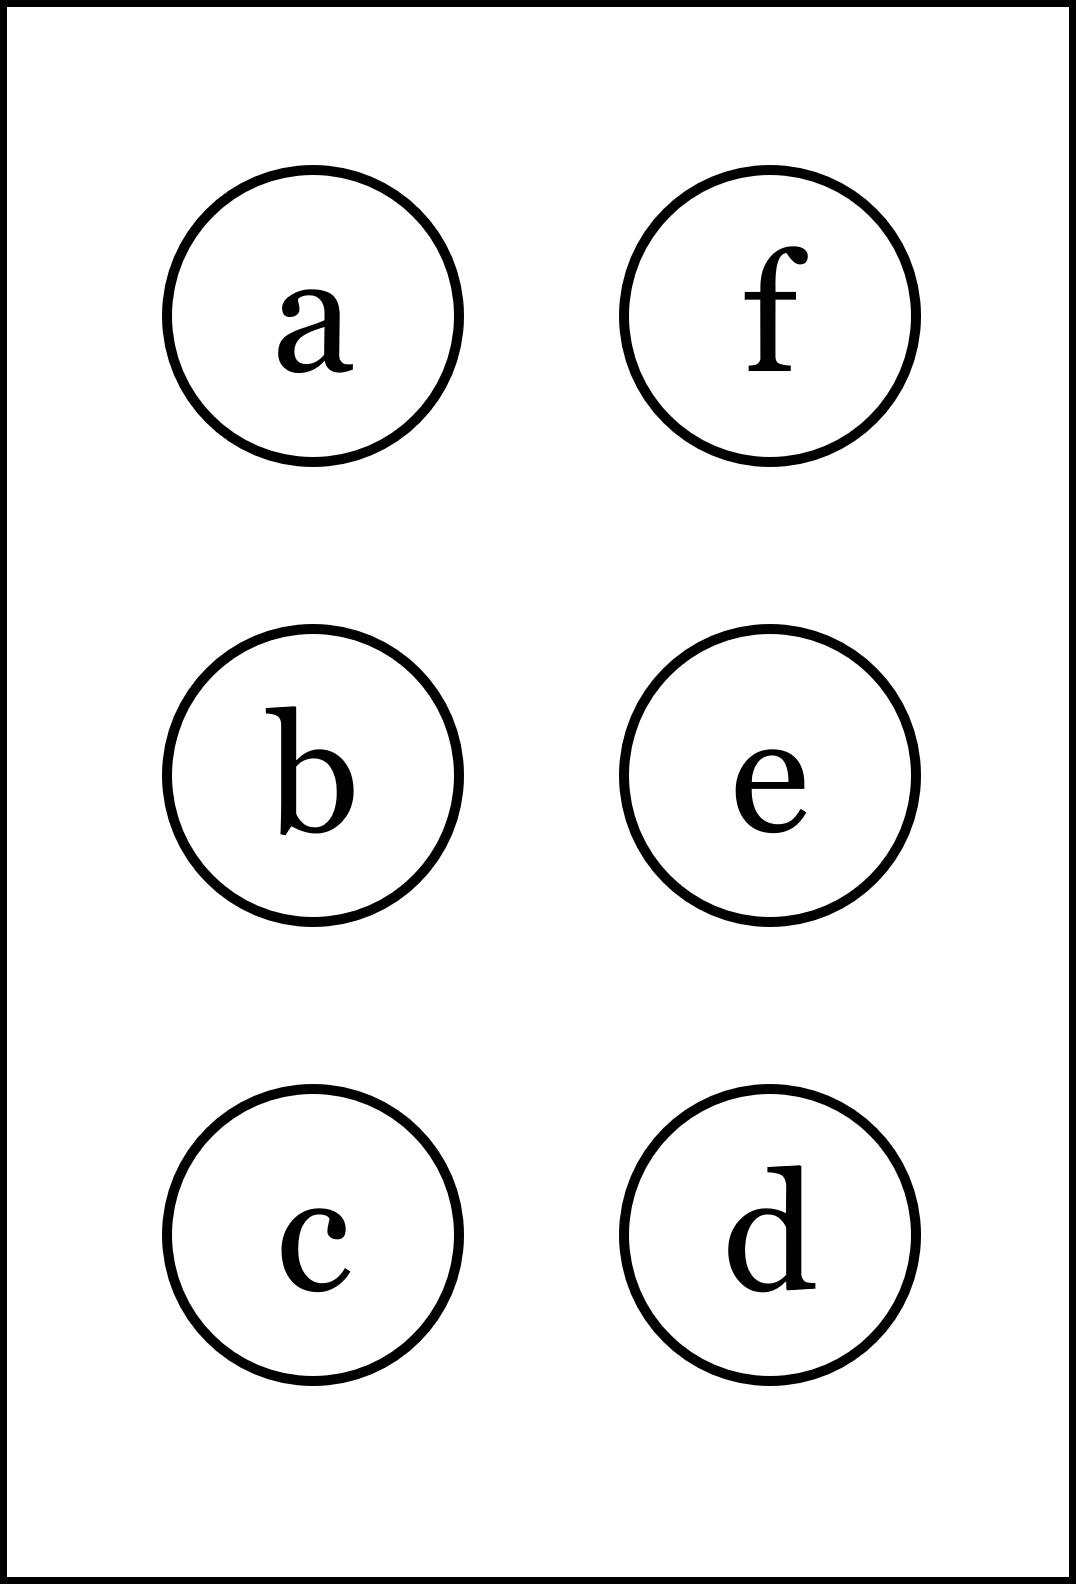
\includegraphics[height=40mm]{../images/braille.png}
{\small Písmeno Braillovej abecedy}
\end{center}
\end{minipage}
\end{center}
\end{minipage}
&
\begin{minipage}[c][104.5mm][t]{0.5\linewidth}
\begin{center}
\vspace{7mm}
{\huge Závorky a zlomky, skupina \textit{Zeta $\zeta$} -\romannumeral4}\\[5mm]
\textit{Jméno:}\phantom{xxxxxxxxxxxxxxxxxxxxxxxxxxxxxxxxxxxxxxxxxxxxxxxxxxxxxxxxxxxxxxxxx}\\[5mm]
\begin{minipage}{0.95\linewidth}
\begin{center}
\textbf{Uprav výrazy (a) až (f)}. Pokud je výraz za otazníky roven výrazu pred otázniky, tak napravo obarvi príslušející kroužek. \textbf{Spolu odevzdejte výsledné slovo.}
\end{center}
\end{minipage}
\\[1mm]
\begin{minipage}{0.79\linewidth}
\begin{center}
\begin{varwidth}{\linewidth}
\begin{enumerate}
\normalsize
\item $6(x+4)-2(-5-4x)$\quad \dotfill\; ???\;\dotfill \quad $14x+34$
\item $2(-6+5x)(5x-8)-6(5+x)$\quad \dotfill\; ???\;\dotfill \quad $50x^2-146x+66$
\item $(2x-1)^3-(5x+1)^2$\quad \dotfill\; ???\;\dotfill \quad $8x^3-37x^2-4x-2$
\item $\cfrac{3x-4}{-6}-2\cfrac{1-8x}{4}$\quad \dotfill\; ???\;\dotfill \quad $\cfrac{-4}{24}$
\item $\cfrac{\frac{-8}{3}-\frac{-7}{x}}{\frac{1}{-3}+\frac{2}{-1}}$\quad \dotfill\; ???\;\dotfill \quad $\cfrac{-24x+63}{-21x}$
\item $\cfrac{(-3+4x)^2-8}{(-x-5)\cdot\frac{1}{x}}$\quad \dotfill\; ???\;\dotfill \quad $\cfrac{16x^3-24x^2-x}{x-5}$
\end{enumerate}
\end{varwidth}
\end{center}
\end{minipage}
\begin{minipage}{0.20\linewidth}
\begin{center}
{\Huge\bfseries 4.} \\[2mm]
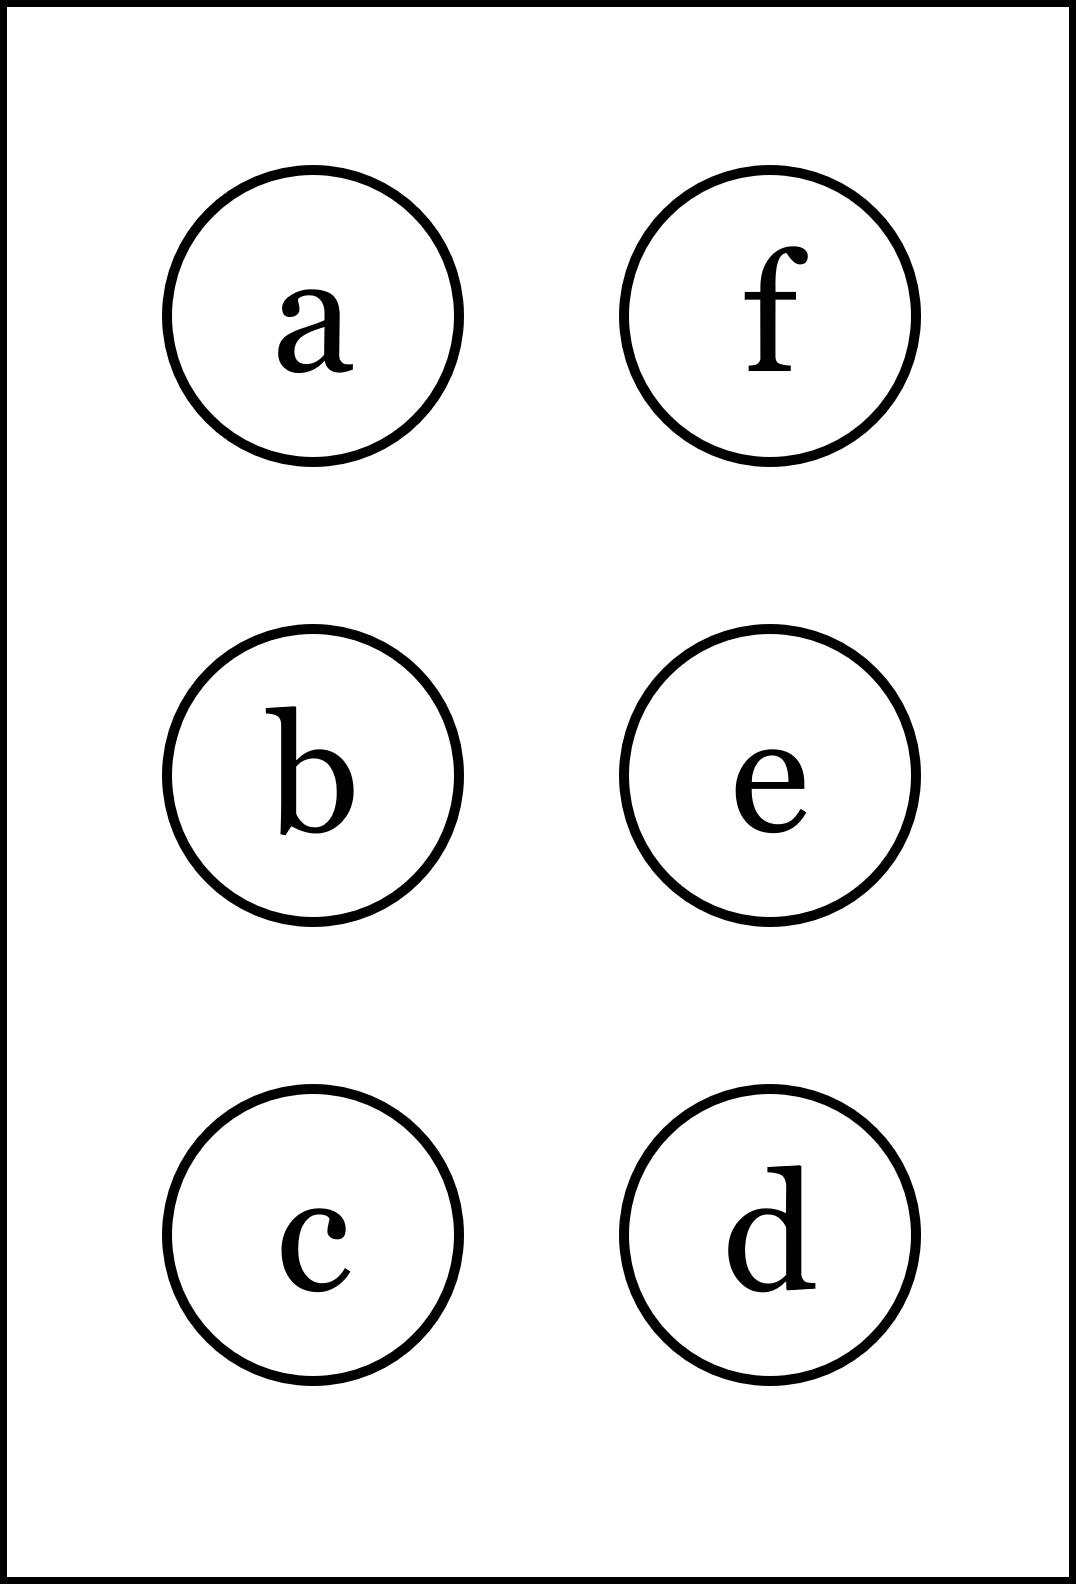
\includegraphics[height=40mm]{../images/braille.png}
{\small Písmeno Braillovej abecedy}
\end{center}
\end{minipage}
\end{center}
\end{minipage}
%
\end{tabular}
\newpage
\thispagestyle{empty}
\begin{tabular}{c:c}
\begin{minipage}[c][104.5mm][t]{0.5\linewidth}
\begin{center}
\vspace{7mm}
{\huge Závorky a zlomky, skupina \textit{Eta $\eta$} -\romannumeral1}\\[5mm]
\textit{Jméno:}\phantom{xxxxxxxxxxxxxxxxxxxxxxxxxxxxxxxxxxxxxxxxxxxxxxxxxxxxxxxxxxxxxxxxx}\\[5mm]
\begin{minipage}{0.95\linewidth}
\begin{center}
\textbf{Uprav výrazy (a) až (f)}. Pokud je výraz za otazníky roven výrazu pred otázniky, tak napravo obarvi príslušející kroužek. \textbf{Spolu odevzdejte výsledné slovo.}
\end{center}
\end{minipage}
\\[1mm]
\begin{minipage}{0.79\linewidth}
\begin{center}
\begin{varwidth}{\linewidth}
\begin{enumerate}
\normalsize
\item $-4(x-3)+4(-2+3x)$\quad \dotfill\; ???\;\dotfill \quad $8x+4$
\item $-5(-4+x)(2x-3)+2(8+6x)$\quad \dotfill\; ???\;\dotfill \quad $-10x^2-67x$
\item $(4x+1)^3-(5x-2)^2$\quad \dotfill\; ???\;\dotfill \quad $64x^3+23x^2+32x-3$
\item $\cfrac{-3x-8}{-2}+5\cfrac{-1+x}{-6}$\quad \dotfill\; ???\;\dotfill \quad $\cfrac{-8x+58}{-12}$
\item $\cfrac{\frac{1}{-2}-\frac{1}{x}}{\frac{1}{-8}+\frac{-4}{3}}$\quad \dotfill\; ???\;\dotfill \quad $\cfrac{-25x-50}{-70x}$
\item $\cfrac{(-6-3x)^2-1}{(-3x-3)\cdot\frac{9}{x}}$\quad \dotfill\; ???\;\dotfill \quad $\cfrac{9x^3+36x^2-35x}{27x-27}$
\end{enumerate}
\end{varwidth}
\end{center}
\end{minipage}
\begin{minipage}{0.20\linewidth}
\begin{center}
{\Huge\bfseries 1.} \\[2mm]
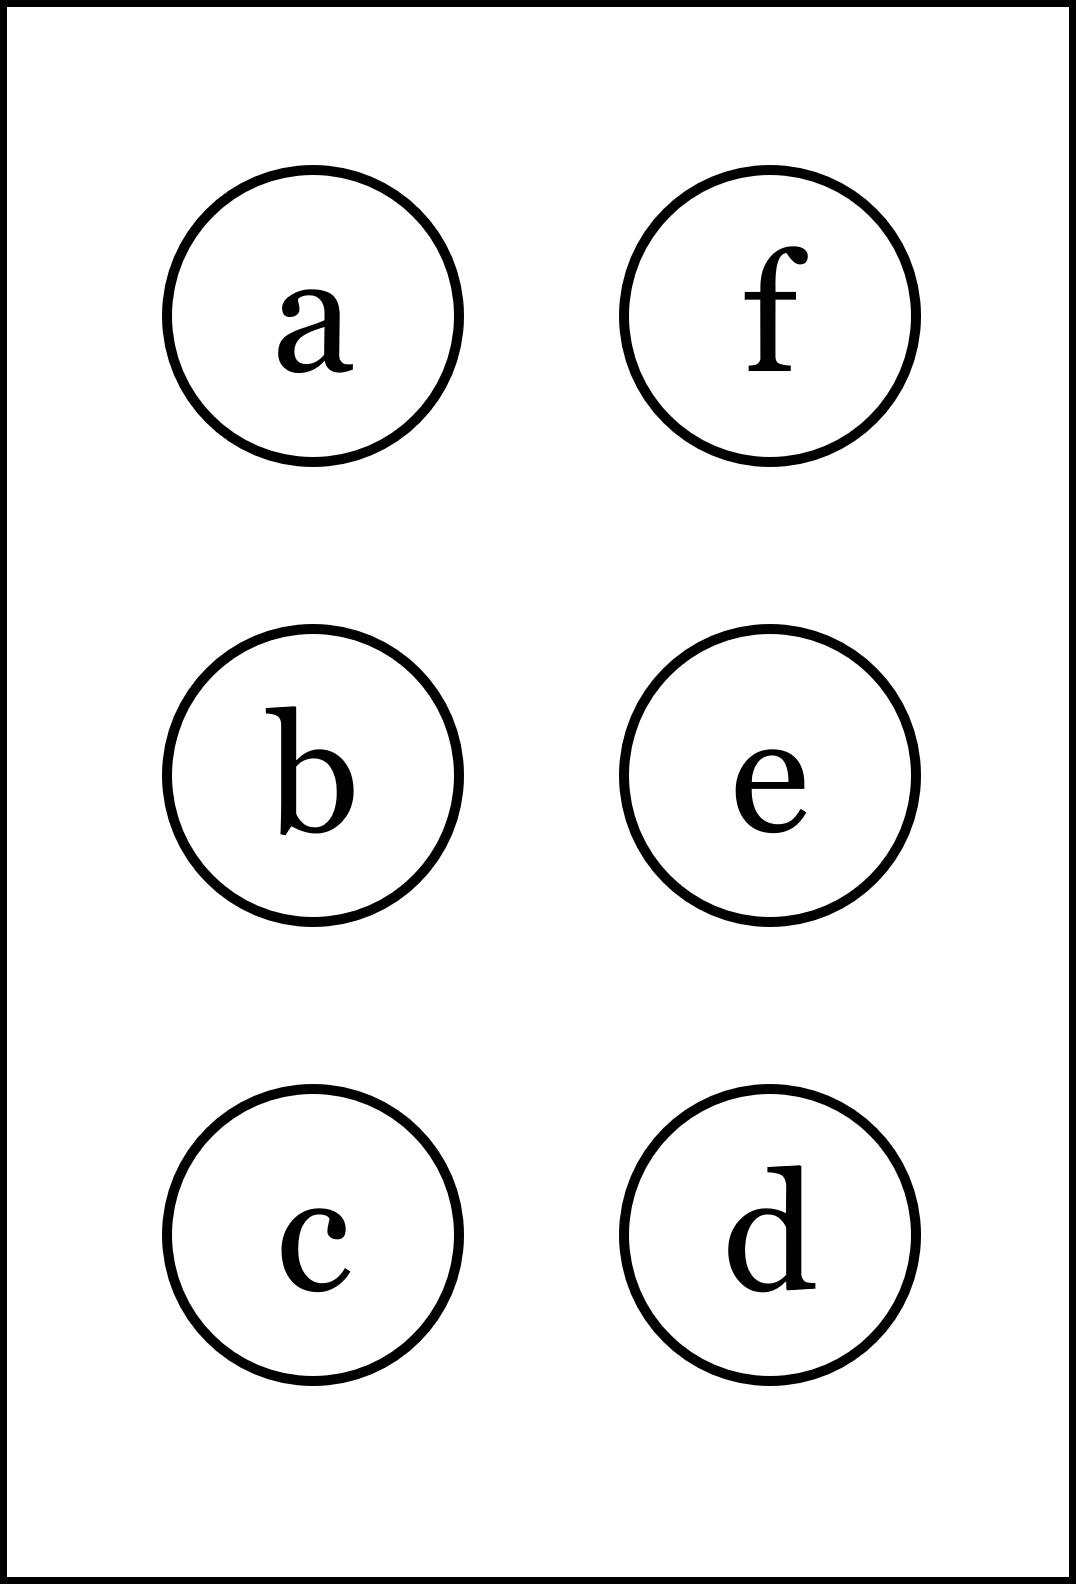
\includegraphics[height=40mm]{../images/braille.png}
{\small Písmeno Braillovej abecedy}
\end{center}
\end{minipage}
\end{center}
\end{minipage}
&
\begin{minipage}[c][104.5mm][t]{0.5\linewidth}
\begin{center}
\vspace{7mm}
{\huge Závorky a zlomky, skupina \textit{Eta $\eta$} -\romannumeral2}\\[5mm]
\textit{Jméno:}\phantom{xxxxxxxxxxxxxxxxxxxxxxxxxxxxxxxxxxxxxxxxxxxxxxxxxxxxxxxxxxxxxxxxx}\\[5mm]
\begin{minipage}{0.95\linewidth}
\begin{center}
\textbf{Uprav výrazy (a) až (f)}. Pokud je výraz za otazníky roven výrazu pred otázniky, tak napravo obarvi príslušející kroužek. \textbf{Spolu odevzdejte výsledné slovo.}
\end{center}
\end{minipage}
\\[1mm]
\begin{minipage}{0.79\linewidth}
\begin{center}
\begin{varwidth}{\linewidth}
\begin{enumerate}
\normalsize
\item $-7(2x-7)+1(3-x)$\quad \dotfill\; ???\;\dotfill \quad $-15x+52$
\item $3(-1+2x)(2x-1)-6(-3+3x)$\quad \dotfill\; ???\;\dotfill \quad $12x^2+30x-21$
\item $(4x-1)^3-(3x-9)^2$\quad \dotfill\; ???\;\dotfill \quad $64x^3-57x^2+66x-82$
\item $\cfrac{-2x-2}{-4}-3\cfrac{1-x}{-4}$\quad \dotfill\; ???\;\dotfill \quad $\cfrac{-4x+20}{-16}$
\item $\cfrac{\frac{6}{-1}-\frac{5}{x}}{\frac{1}{3}+\frac{4}{-2}}$\quad \dotfill\; ???\;\dotfill \quad $\cfrac{-36x-30}{-10x}$
\item $\cfrac{(-2+3x)^2-6}{(-2x-1)\cdot\frac{1}{x}}$\quad \dotfill\; ???\;\dotfill \quad $\cfrac{9x^3-12x^2+2x}{2x-1}$
\end{enumerate}
\end{varwidth}
\end{center}
\end{minipage}
\begin{minipage}{0.20\linewidth}
\begin{center}
{\Huge\bfseries 2.} \\[2mm]
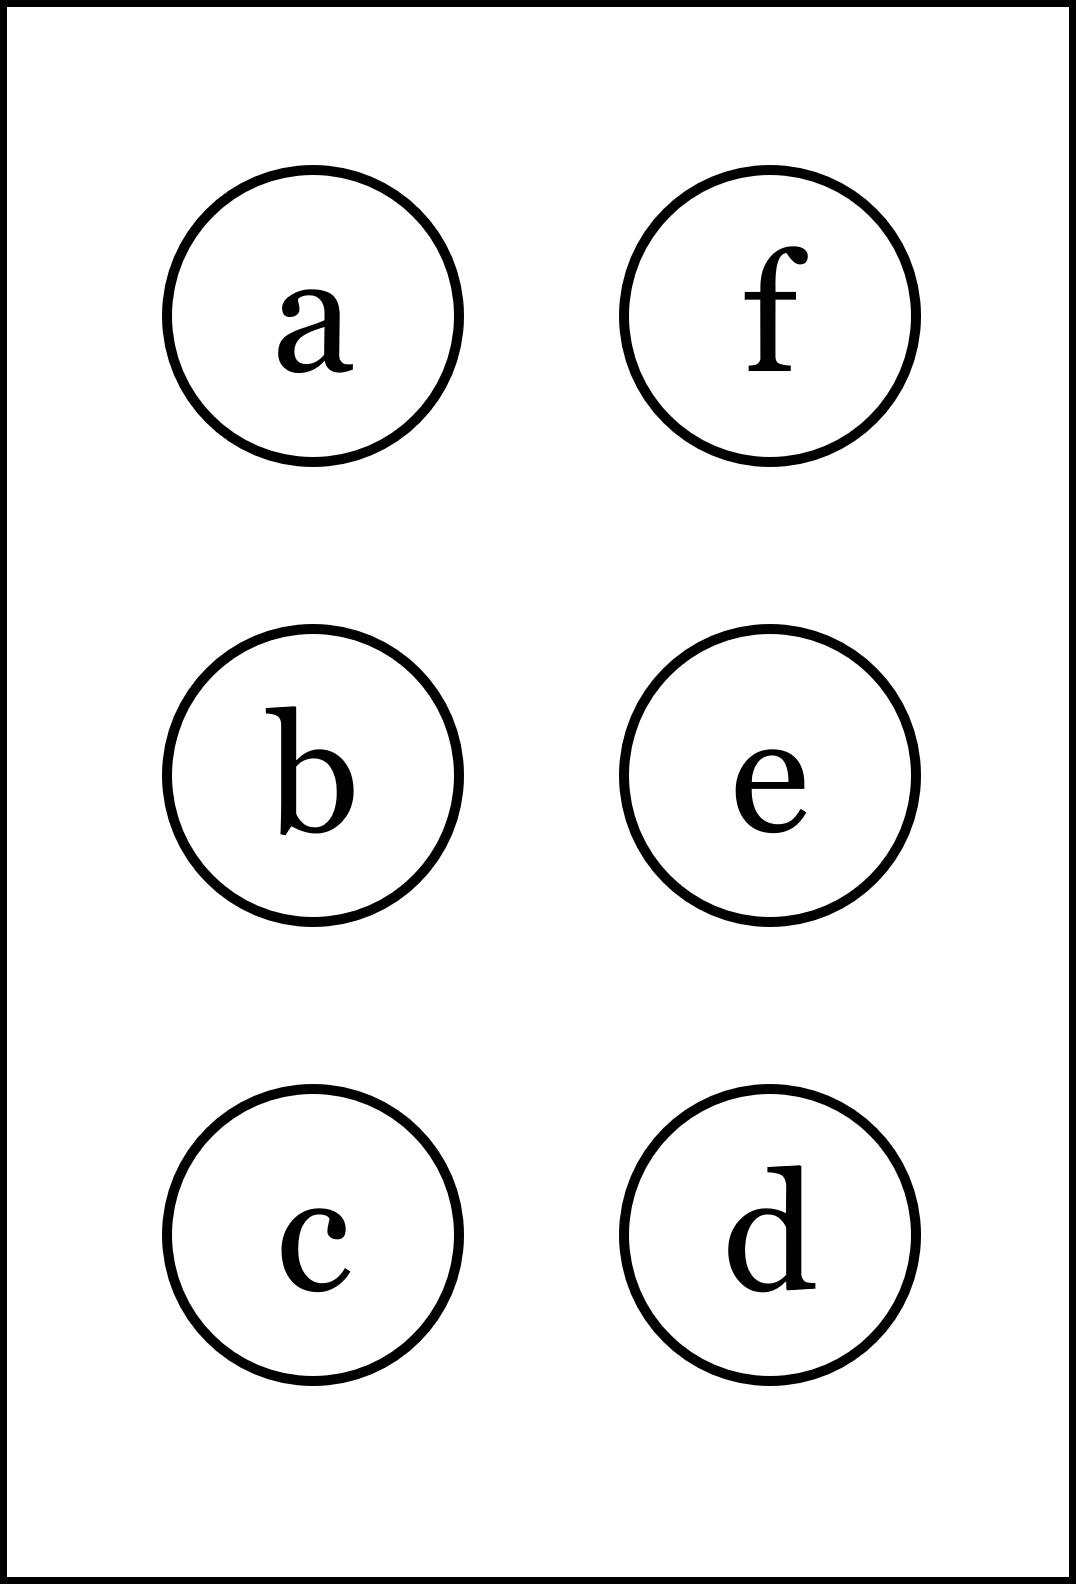
\includegraphics[height=40mm]{../images/braille.png}
{\small Písmeno Braillovej abecedy}
\end{center}
\end{minipage}
\end{center}
\end{minipage}
\\ \hdashline
\begin{minipage}[c][104.5mm][t]{0.5\linewidth}
\begin{center}
\vspace{7mm}
{\huge Závorky a zlomky, skupina \textit{Eta $\eta$} -\romannumeral3}\\[5mm]
\textit{Jméno:}\phantom{xxxxxxxxxxxxxxxxxxxxxxxxxxxxxxxxxxxxxxxxxxxxxxxxxxxxxxxxxxxxxxxxx}\\[5mm]
\begin{minipage}{0.95\linewidth}
\begin{center}
\textbf{Uprav výrazy (a) až (f)}. Pokud je výraz za otazníky roven výrazu pred otázniky, tak napravo obarvi príslušející kroužek. \textbf{Spolu odevzdejte výsledné slovo.}
\end{center}
\end{minipage}
\\[1mm]
\begin{minipage}{0.79\linewidth}
\begin{center}
\begin{varwidth}{\linewidth}
\begin{enumerate}
\normalsize
\item $7(3x+9)-2(-2+7x)$\quad \dotfill\; ???\;\dotfill \quad $7x+67$
\item $4(1-2x)(2x-1)+5(-2+5x)$\quad \dotfill\; ???\;\dotfill \quad $-16x^2+41x-14$
\item $(-2x-3)^3-(3x+1)^2$\quad \dotfill\; ???\;\dotfill \quad $-8x^3-45x^2-60x-28$
\item $\cfrac{4x-4}{2}-6\cfrac{-3-5x}{-6}$\quad \dotfill\; ???\;\dotfill \quad $\cfrac{36x+60}{12}$
\item $\cfrac{\frac{3}{3}-\frac{1}{x}}{\frac{1}{-8}+\frac{-1}{-4}}$\quad \dotfill\; ???\;\dotfill \quad $\cfrac{94x-95}{12x}$
\item $\cfrac{(2+2x)^2+1}{(7x-5)\cdot\frac{1}{x}}$\quad \dotfill\; ???\;\dotfill \quad $\cfrac{4x^3+8x^2-5x}{-7x-5}$
\end{enumerate}
\end{varwidth}
\end{center}
\end{minipage}
\begin{minipage}{0.20\linewidth}
\begin{center}
{\Huge\bfseries 3.} \\[2mm]
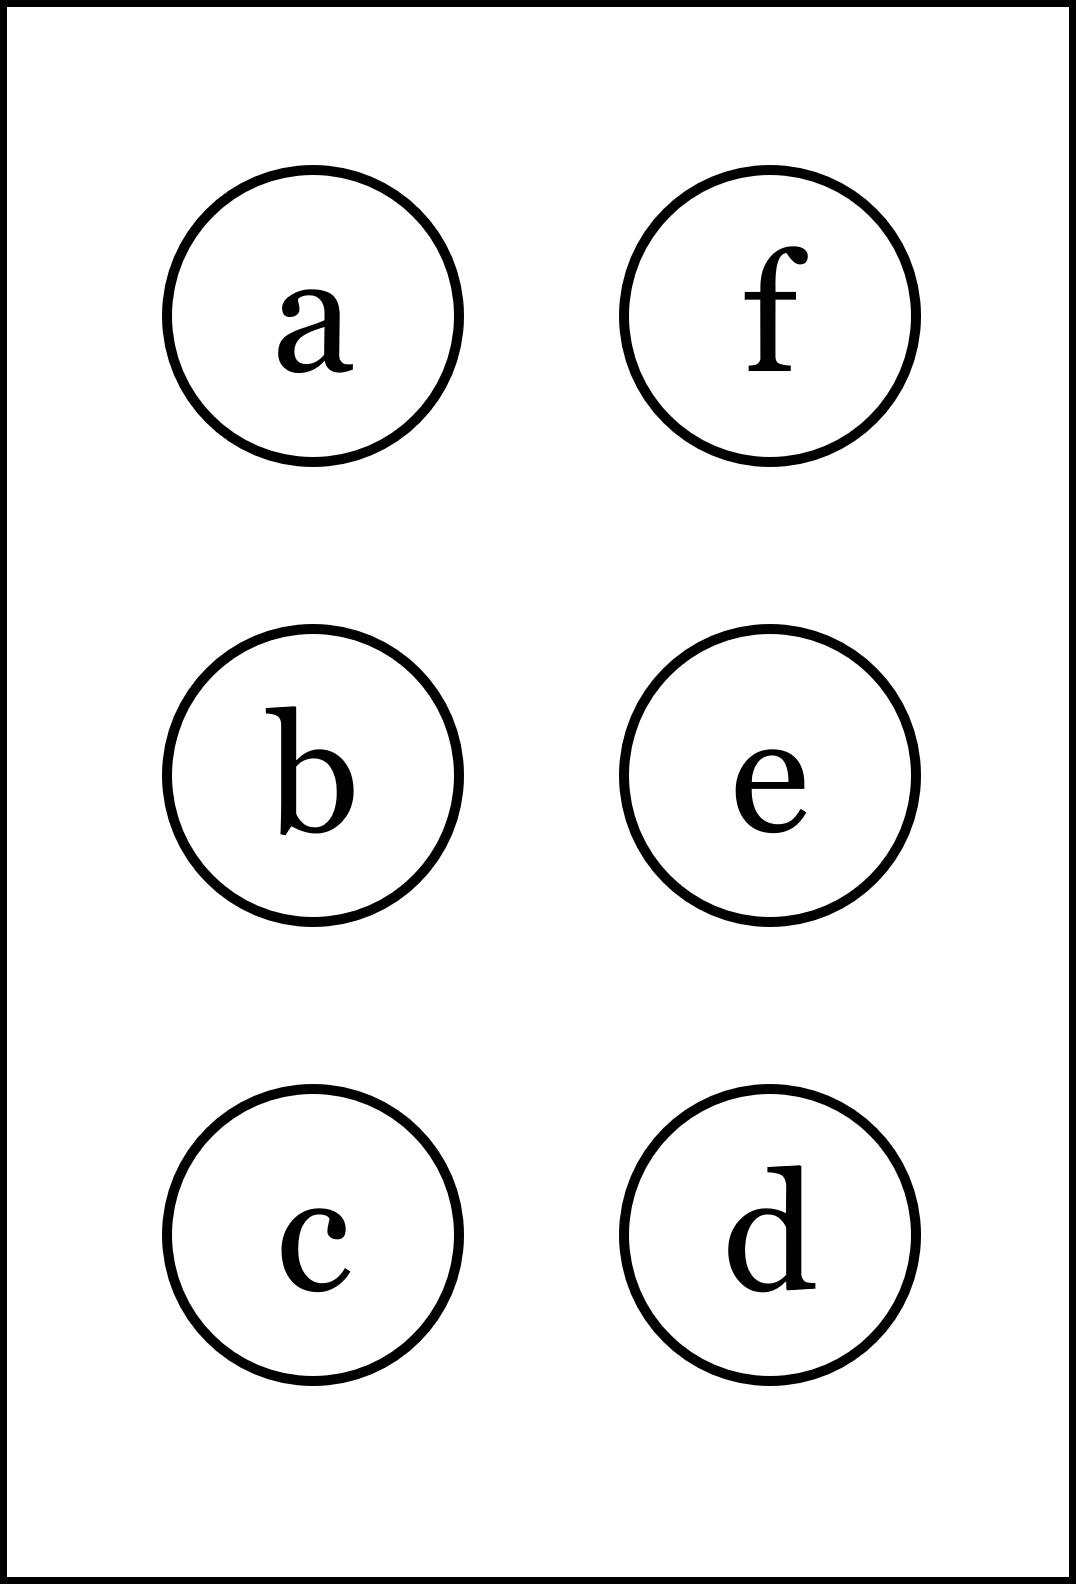
\includegraphics[height=40mm]{../images/braille.png}
{\small Písmeno Braillovej abecedy}
\end{center}
\end{minipage}
\end{center}
\end{minipage}
&
\begin{minipage}[c][104.5mm][t]{0.5\linewidth}
\begin{center}
\vspace{7mm}
{\huge Závorky a zlomky, skupina \textit{Eta $\eta$} -\romannumeral4}\\[5mm]
\textit{Jméno:}\phantom{xxxxxxxxxxxxxxxxxxxxxxxxxxxxxxxxxxxxxxxxxxxxxxxxxxxxxxxxxxxxxxxxx}\\[5mm]
\begin{minipage}{0.95\linewidth}
\begin{center}
\textbf{Uprav výrazy (a) až (f)}. Pokud je výraz za otazníky roven výrazu pred otázniky, tak napravo obarvi príslušející kroužek. \textbf{Spolu odevzdejte výsledné slovo.}
\end{center}
\end{minipage}
\\[1mm]
\begin{minipage}{0.79\linewidth}
\begin{center}
\begin{varwidth}{\linewidth}
\begin{enumerate}
\normalsize
\item $4(-x-7)-7(7-5x)$\quad \dotfill\; ???\;\dotfill \quad $31x-77$
\item $5(2-2x)(-2x+5)-3(-2-3x)$\quad \dotfill\; ???\;\dotfill \quad $20x^2+61x-56$
\item $(-2x+4)^3-(4x-4)^2$\quad \dotfill\; ???\;\dotfill \quad $-8x^3+32x^2-64x+48$
\item $\cfrac{5x+6}{-3}+5\cfrac{6+5x}{-2}$\quad \dotfill\; ???\;\dotfill \quad $\cfrac{85x-102}{-6}$
\item $\cfrac{\frac{3}{-5}-\frac{-2}{x}}{\frac{1}{-1}+\frac{4}{1}}$\quad \dotfill\; ???\;\dotfill \quad $\cfrac{-3x+10}{15x}$
\item $\cfrac{(-5+x)^2+3}{(-7x-2)\cdot\frac{1}{x}}$\quad \dotfill\; ???\;\dotfill \quad $\cfrac{x^3-10x^2-28x}{7x-2}$
\end{enumerate}
\end{varwidth}
\end{center}
\end{minipage}
\begin{minipage}{0.20\linewidth}
\begin{center}
{\Huge\bfseries 4.} \\[2mm]
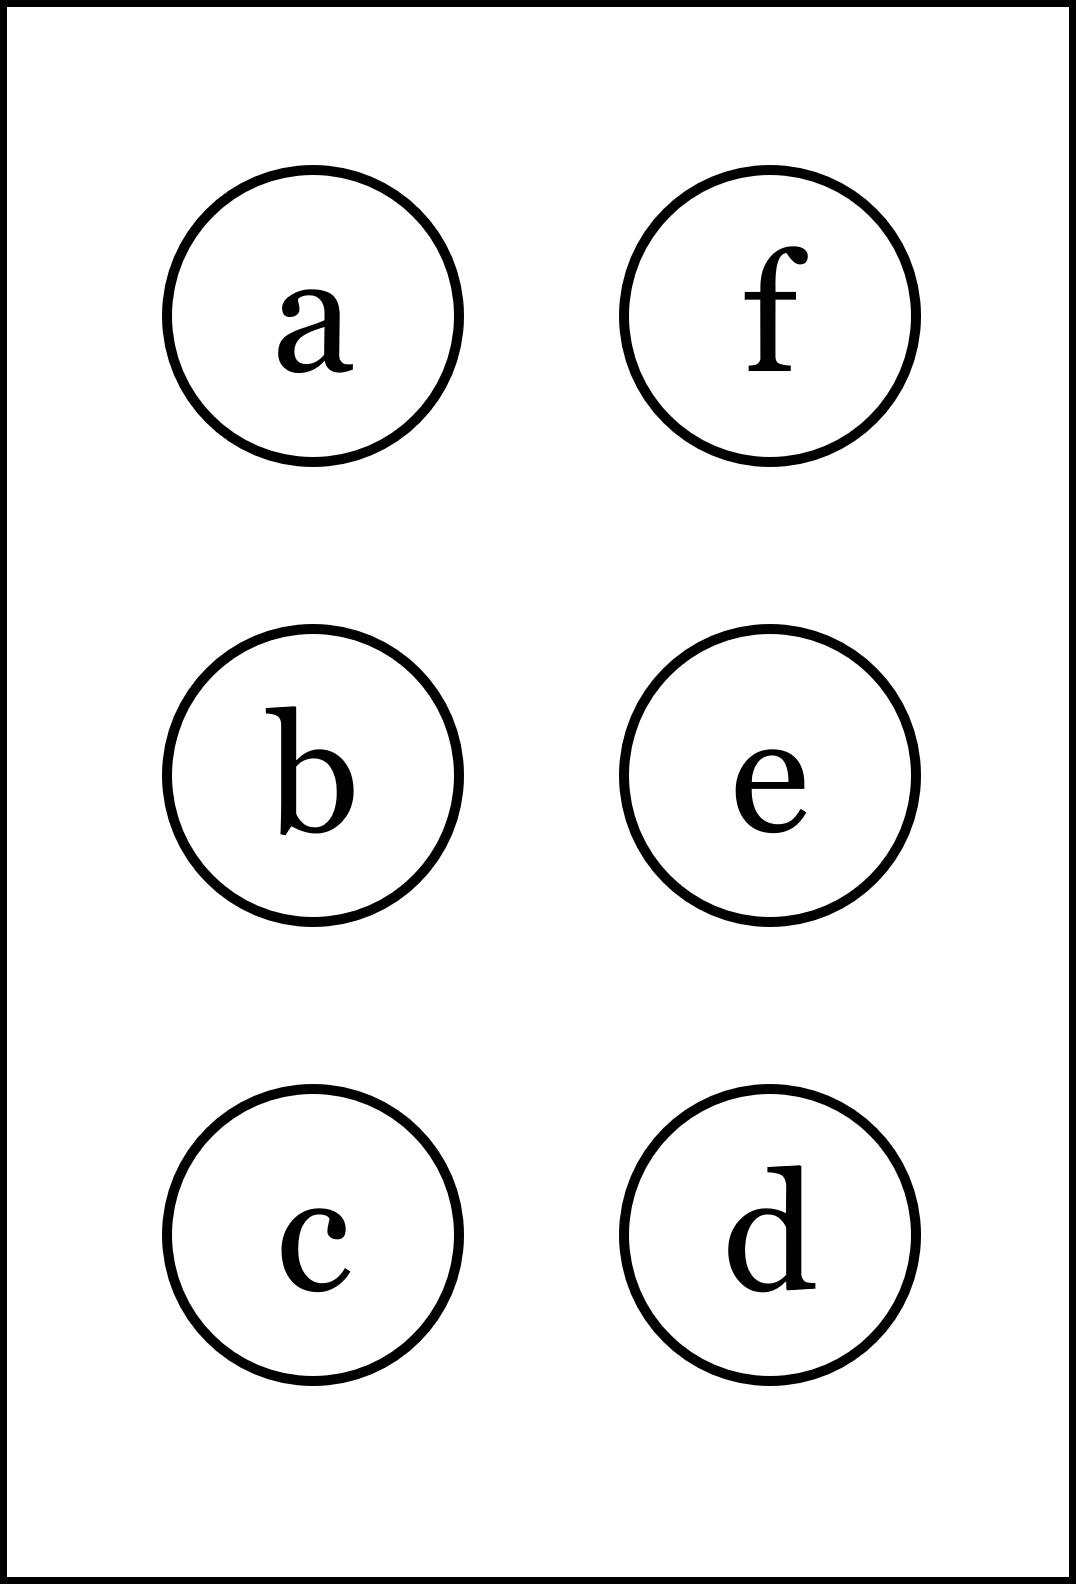
\includegraphics[height=40mm]{../images/braille.png}
{\small Písmeno Braillovej abecedy}
\end{center}
\end{minipage}
\end{center}
\end{minipage}
%
\end{tabular}
\newpage
\thispagestyle{empty}
\begin{tabular}{c:c}
\begin{minipage}[c][104.5mm][t]{0.5\linewidth}
\begin{center}
\vspace{7mm}
{\huge Závorky a zlomky, skupina \textit{Theta $\theta$} -\romannumeral1}\\[5mm]
\textit{Jméno:}\phantom{xxxxxxxxxxxxxxxxxxxxxxxxxxxxxxxxxxxxxxxxxxxxxxxxxxxxxxxxxxxxxxxxx}\\[5mm]
\begin{minipage}{0.95\linewidth}
\begin{center}
\textbf{Uprav výrazy (a) až (f)}. Pokud je výraz za otazníky roven výrazu pred otázniky, tak napravo obarvi príslušející kroužek. \textbf{Spolu odevzdejte výsledné slovo.}
\end{center}
\end{minipage}
\\[1mm]
\begin{minipage}{0.79\linewidth}
\begin{center}
\begin{varwidth}{\linewidth}
\begin{enumerate}
\normalsize
\item $-4(5x+3)-6(-8+4x)$\quad \dotfill\; ???\;\dotfill \quad $-44x+36$
\item $3(-4-2x)(3x+2)-2(-1-5x)$\quad \dotfill\; ???\;\dotfill \quad $-18x^2+38x-22$
\item $(3x-3)^3-(6x+5)^2$\quad \dotfill\; ???\;\dotfill \quad $-27x^3-117x^2-52$
\item $\cfrac{7x+5}{-2}+2\cfrac{-5-6x}{-4}$\quad \dotfill\; ???\;\dotfill \quad $\cfrac{-4x}{8}$
\item $\cfrac{\frac{2}{-3}-\frac{-3}{x}}{\frac{1}{1}+\frac{-5}{2}}$\quad \dotfill\; ???\;\dotfill \quad $\cfrac{x-15}{9x}$
\item $\cfrac{(1+5x)^2-3}{(x-1)\cdot\frac{-2}{x}}$\quad \dotfill\; ???\;\dotfill \quad $\cfrac{25x^3+10x^2-2x}{-2x+2}$
\end{enumerate}
\end{varwidth}
\end{center}
\end{minipage}
\begin{minipage}{0.20\linewidth}
\begin{center}
{\Huge\bfseries 1.} \\[2mm]
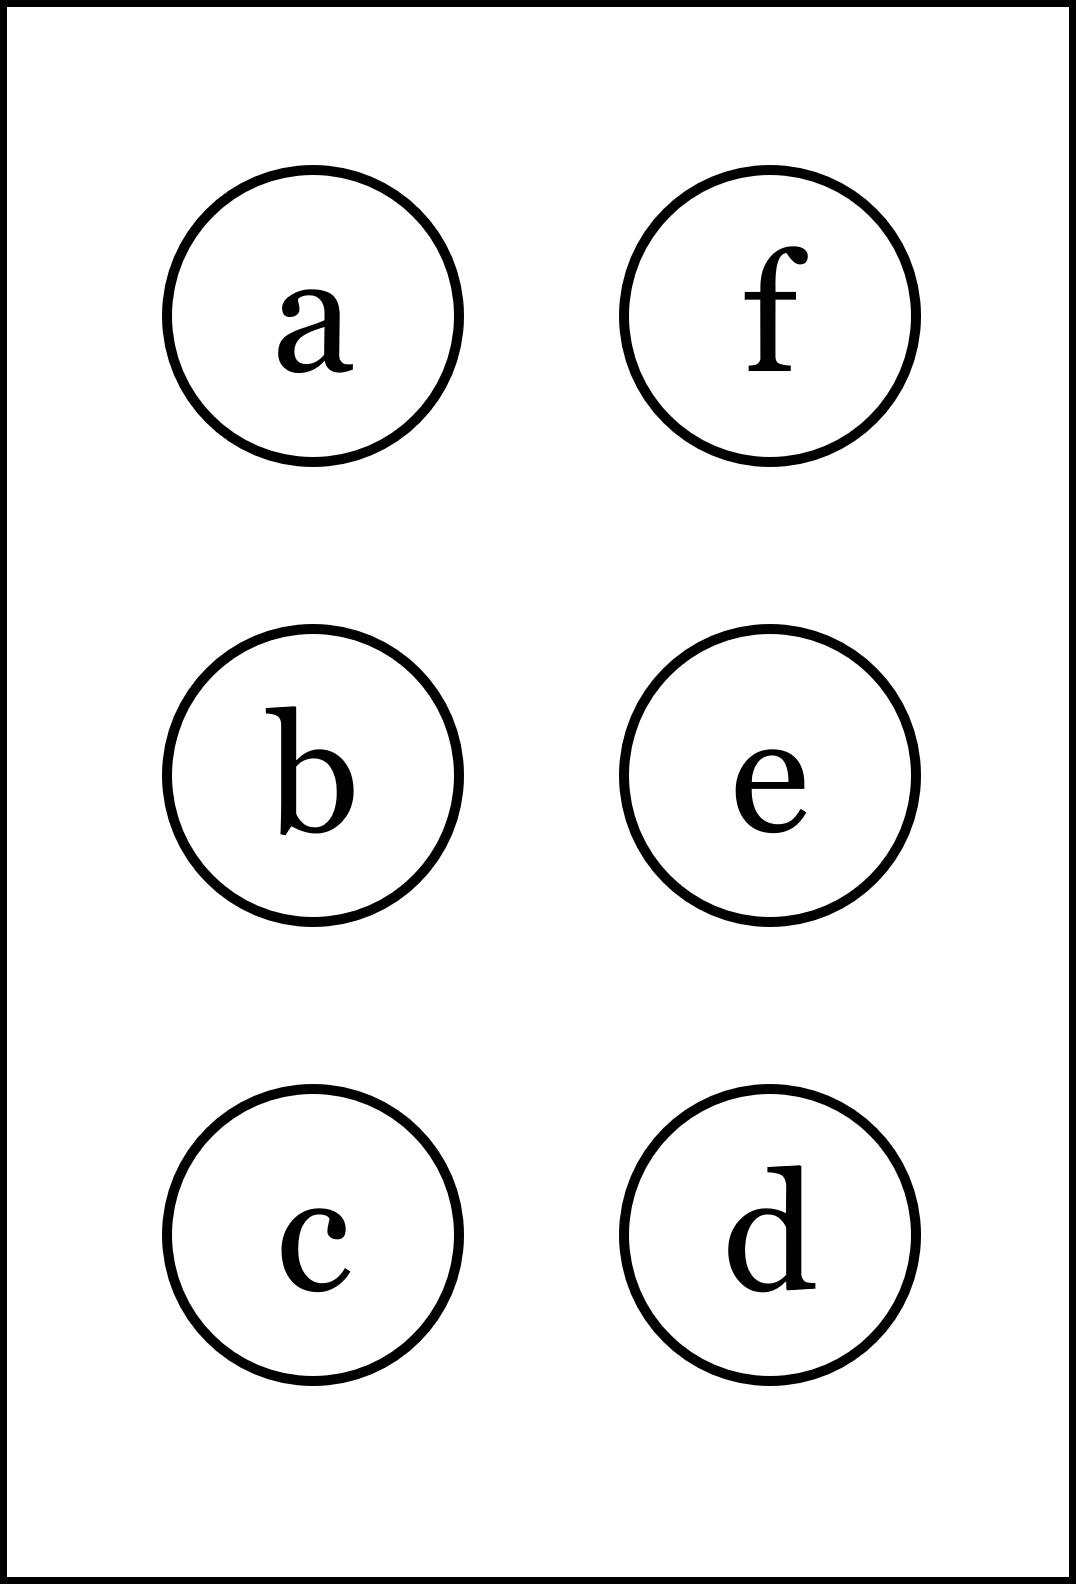
\includegraphics[height=40mm]{../images/braille.png}
{\small Písmeno Braillovej abecedy}
\end{center}
\end{minipage}
\end{center}
\end{minipage}
&
\begin{minipage}[c][104.5mm][t]{0.5\linewidth}
\begin{center}
\vspace{7mm}
{\huge Závorky a zlomky, skupina \textit{Theta $\theta$} -\romannumeral2}\\[5mm]
\textit{Jméno:}\phantom{xxxxxxxxxxxxxxxxxxxxxxxxxxxxxxxxxxxxxxxxxxxxxxxxxxxxxxxxxxxxxxxxx}\\[5mm]
\begin{minipage}{0.95\linewidth}
\begin{center}
\textbf{Uprav výrazy (a) až (f)}. Pokud je výraz za otazníky roven výrazu pred otázniky, tak napravo obarvi príslušející kroužek. \textbf{Spolu odevzdejte výsledné slovo.}
\end{center}
\end{minipage}
\\[1mm]
\begin{minipage}{0.79\linewidth}
\begin{center}
\begin{varwidth}{\linewidth}
\begin{enumerate}
\normalsize
\item $6(7x-8)-2(1+4x)$\quad \dotfill\; ???\;\dotfill \quad $34x-50$
\item $5(6-2x)(x-3)-1(8+2x)$\quad \dotfill\; ???\;\dotfill \quad $-10x^2-58x-98$
\item $(-2x+1)^3-(-x-1)^2$\quad \dotfill\; ???\;\dotfill \quad $8x^3+11x^2-8x$
\item $\cfrac{-3x-5}{-2}-3\cfrac{8+2x}{-6}$\quad \dotfill\; ???\;\dotfill \quad $\cfrac{78}{-12}$
\item $\cfrac{\frac{8}{2}-\frac{3}{x}}{\frac{1}{-1}+\frac{4}{-1}}$\quad \dotfill\; ???\;\dotfill \quad $\cfrac{8x-6}{-10x}$
\item $\cfrac{(-2+2x)^2+6}{(-7x-2)\cdot\frac{9}{x}}$\quad \dotfill\; ???\;\dotfill \quad $\cfrac{4x^3-8x^2-10x}{63x-18}$
\end{enumerate}
\end{varwidth}
\end{center}
\end{minipage}
\begin{minipage}{0.20\linewidth}
\begin{center}
{\Huge\bfseries 2.} \\[2mm]
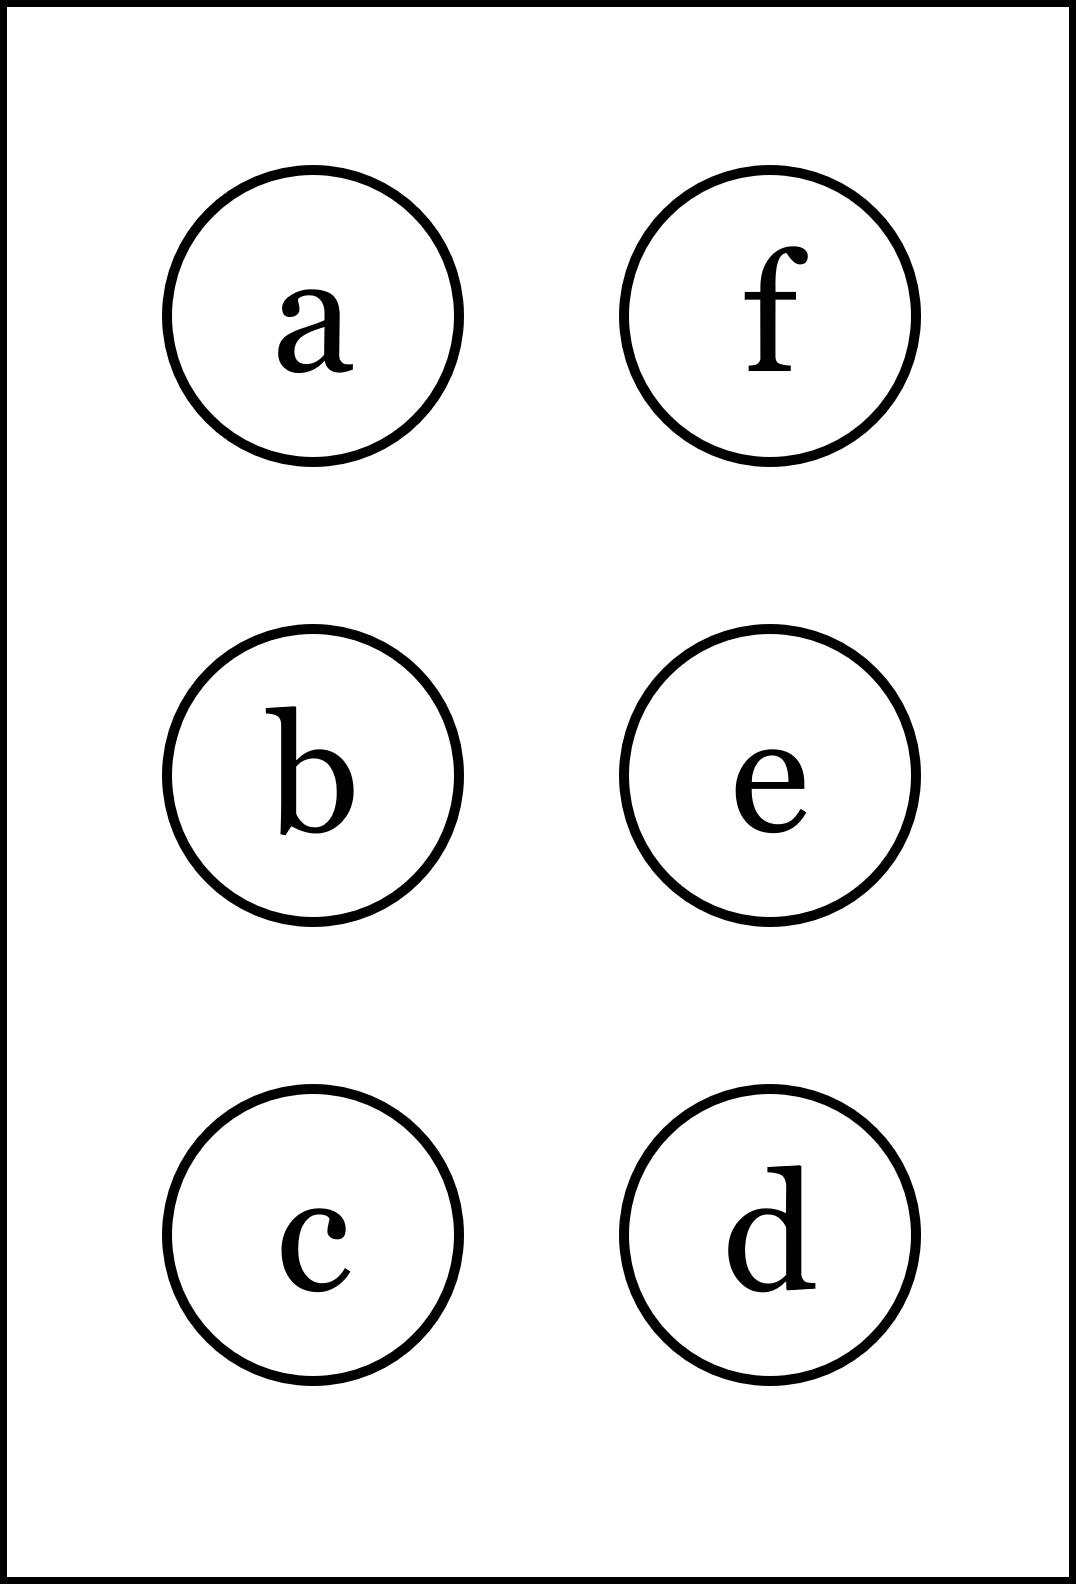
\includegraphics[height=40mm]{../images/braille.png}
{\small Písmeno Braillovej abecedy}
\end{center}
\end{minipage}
\end{center}
\end{minipage}
\\ \hdashline
\begin{minipage}[c][104.5mm][t]{0.5\linewidth}
\begin{center}
\vspace{7mm}
{\huge Závorky a zlomky, skupina \textit{Theta $\theta$} -\romannumeral3}\\[5mm]
\textit{Jméno:}\phantom{xxxxxxxxxxxxxxxxxxxxxxxxxxxxxxxxxxxxxxxxxxxxxxxxxxxxxxxxxxxxxxxxx}\\[5mm]
\begin{minipage}{0.95\linewidth}
\begin{center}
\textbf{Uprav výrazy (a) až (f)}. Pokud je výraz za otazníky roven výrazu pred otázniky, tak napravo obarvi príslušející kroužek. \textbf{Spolu odevzdejte výsledné slovo.}
\end{center}
\end{minipage}
\\[1mm]
\begin{minipage}{0.79\linewidth}
\begin{center}
\begin{varwidth}{\linewidth}
\begin{enumerate}
\normalsize
\item $2(-5x-6)+2(-4+x)$\quad \dotfill\; ???\;\dotfill \quad $-8x-20$
\item $-6(-1+2x)(-x-4)+3(-1-5x)$\quad \dotfill\; ???\;\dotfill \quad $12x^2+27x-27$
\item $(-3x-3)^3-(-x+1)^2$\quad \dotfill\; ???\;\dotfill \quad $-27x^3-82x^2-79x-28$
\item $\cfrac{x+1}{-2}-2\cfrac{-7-3x}{9}$\quad \dotfill\; ???\;\dotfill \quad $\cfrac{-19}{18}$
\item $\cfrac{\frac{-3}{1}-\frac{-1}{x}}{\frac{1}{-1}+\frac{-4}{-5}}$\quad \dotfill\; ???\;\dotfill \quad $\cfrac{-12x+8}{-x}$
\item $\cfrac{(3+2x)^2+1}{(2x+2)\cdot\frac{2}{x}}$\quad \dotfill\; ???\;\dotfill \quad $\cfrac{4x^3+12x^2-10x}{-4x+4}$
\end{enumerate}
\end{varwidth}
\end{center}
\end{minipage}
\begin{minipage}{0.20\linewidth}
\begin{center}
{\Huge\bfseries 3.} \\[2mm]
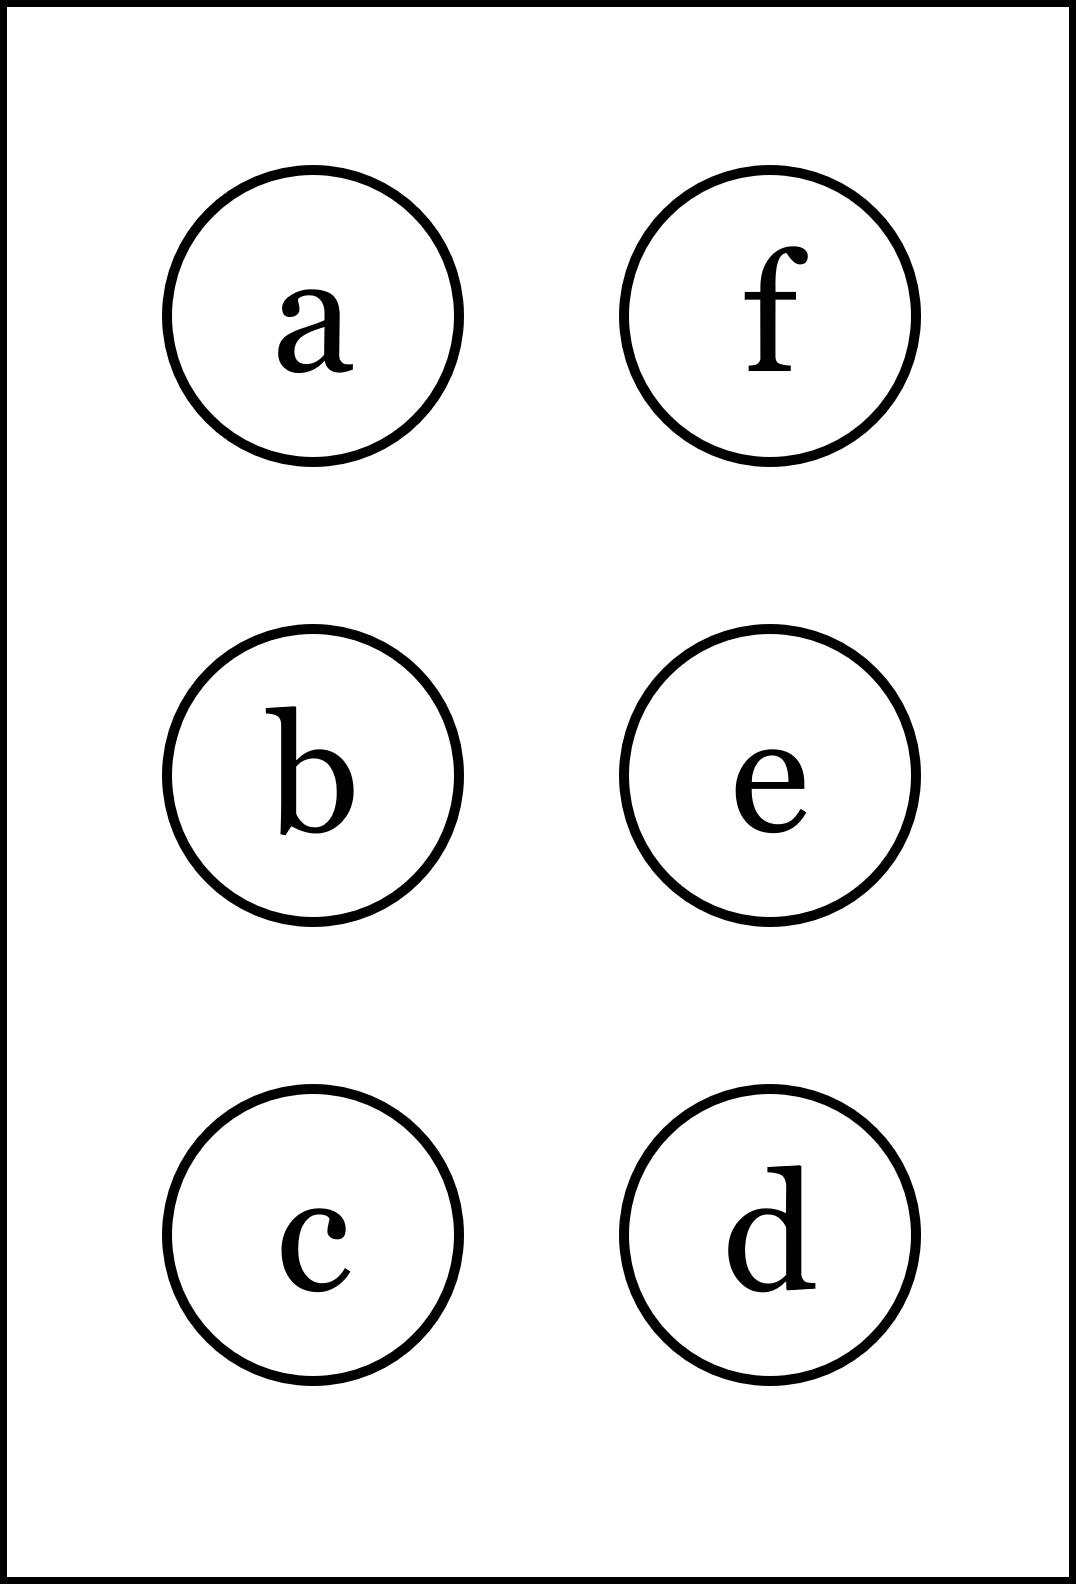
\includegraphics[height=40mm]{../images/braille.png}
{\small Písmeno Braillovej abecedy}
\end{center}
\end{minipage}
\end{center}
\end{minipage}
&
\begin{minipage}[c][104.5mm][t]{0.5\linewidth}
\begin{center}
\vspace{7mm}
{\huge Závorky a zlomky, skupina \textit{Theta $\theta$} -\romannumeral4}\\[5mm]
\textit{Jméno:}\phantom{xxxxxxxxxxxxxxxxxxxxxxxxxxxxxxxxxxxxxxxxxxxxxxxxxxxxxxxxxxxxxxxxx}\\[5mm]
\begin{minipage}{0.95\linewidth}
\begin{center}
\textbf{Uprav výrazy (a) až (f)}. Pokud je výraz za otazníky roven výrazu pred otázniky, tak napravo obarvi príslušející kroužek. \textbf{Spolu odevzdejte výsledné slovo.}
\end{center}
\end{minipage}
\\[1mm]
\begin{minipage}{0.79\linewidth}
\begin{center}
\begin{varwidth}{\linewidth}
\begin{enumerate}
\normalsize
\item $-5(7x+6)-3(5-x)$\quad \dotfill\; ???\;\dotfill \quad $-32x-45$
\item $-2(-6-2x)(x+3)-1(1-5x)$\quad \dotfill\; ???\;\dotfill \quad $4x^2-29x$
\item $(2x-4)^3-(-5x-5)^2$\quad \dotfill\; ???\;\dotfill \quad $8x^3-73x^2+46x-89$
\item $\cfrac{-3x+3}{4}+2\cfrac{2-6x}{6}$\quad \dotfill\; ???\;\dotfill \quad $\cfrac{66x+34}{-24}$
\item $\cfrac{\frac{-1}{-2}-\frac{1}{x}}{\frac{1}{3}+\frac{4}{-1}}$\quad \dotfill\; ???\;\dotfill \quad $\cfrac{3x-6}{-22x}$
\item $\cfrac{(-8+4x)^2+6}{(-x+1)\cdot\frac{5}{x}}$\quad \dotfill\; ???\;\dotfill \quad $\cfrac{16x^3-64x^2-70x}{5x+5}$
\end{enumerate}
\end{varwidth}
\end{center}
\end{minipage}
\begin{minipage}{0.20\linewidth}
\begin{center}
{\Huge\bfseries 4.} \\[2mm]
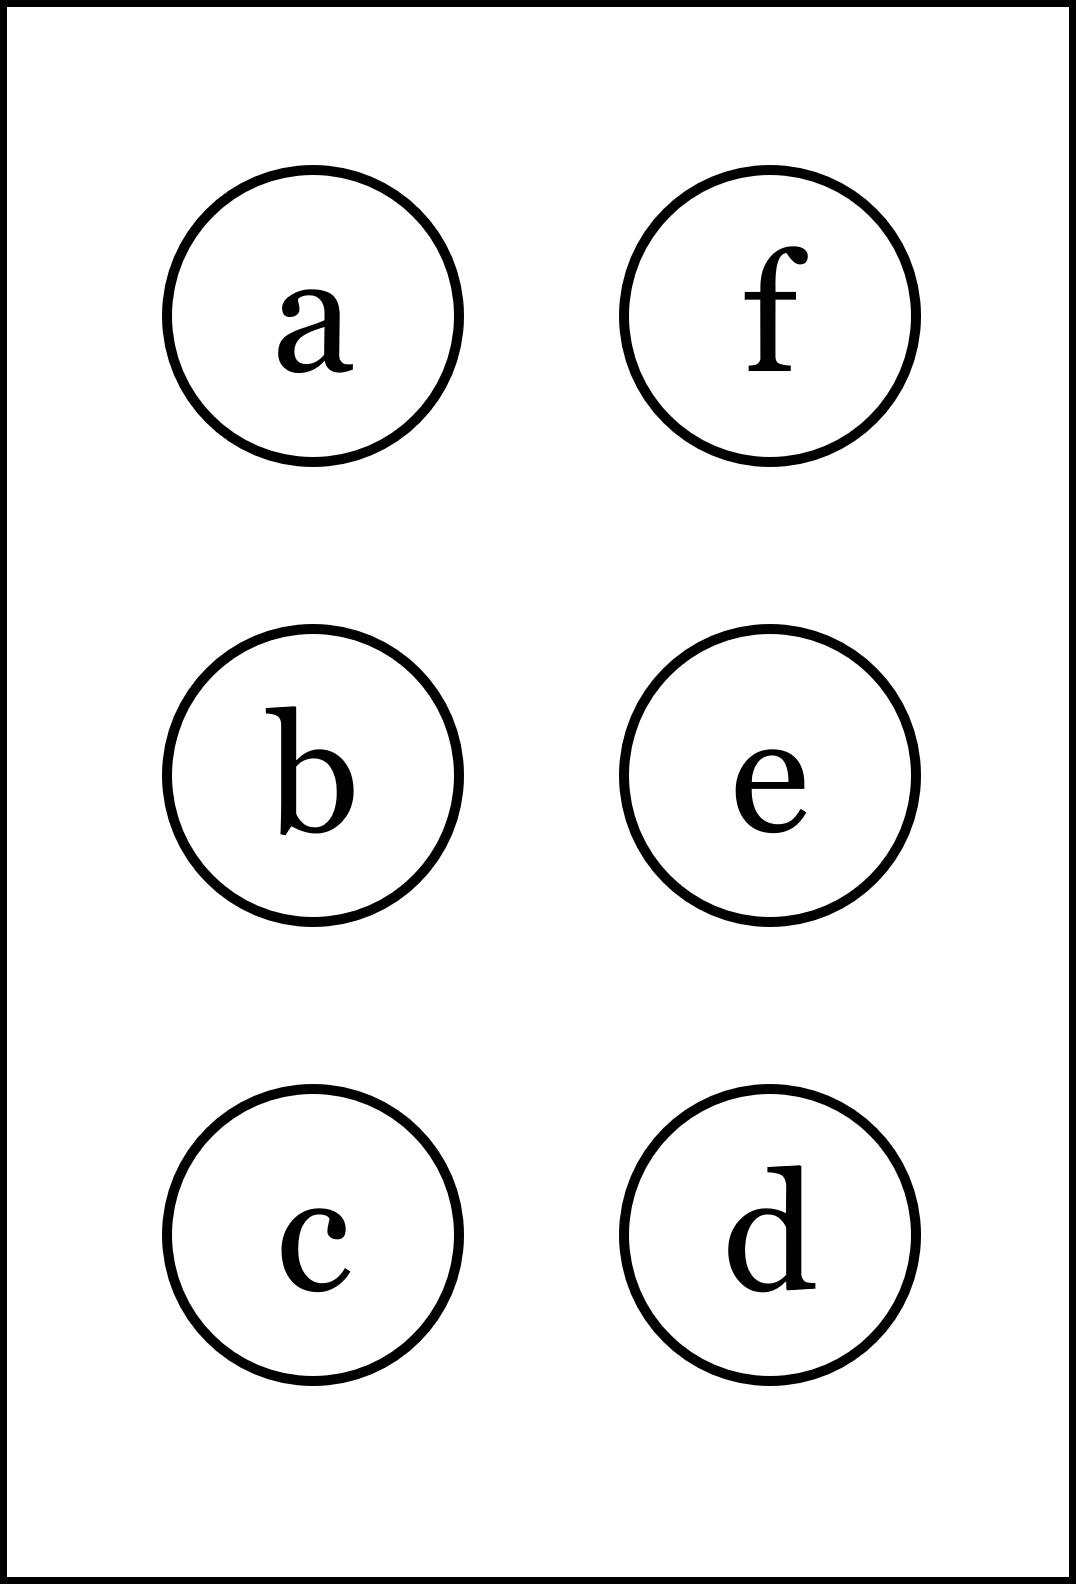
\includegraphics[height=40mm]{../images/braille.png}
{\small Písmeno Braillovej abecedy}
\end{center}
\end{minipage}
\end{center}
\end{minipage}
%
\end{tabular}
\newpage
\thispagestyle{empty}
\begin{tabular}{c:c}
\begin{minipage}[c][104.5mm][t]{0.5\linewidth}
\begin{center}
\vspace{7mm}
{\huge Závorky a zlomky, skupina \textit{Iota $\iota$} -\romannumeral1}\\[5mm]
\textit{Jméno:}\phantom{xxxxxxxxxxxxxxxxxxxxxxxxxxxxxxxxxxxxxxxxxxxxxxxxxxxxxxxxxxxxxxxxx}\\[5mm]
\begin{minipage}{0.95\linewidth}
\begin{center}
\textbf{Uprav výrazy (a) až (f)}. Pokud je výraz za otazníky roven výrazu pred otázniky, tak napravo obarvi príslušející kroužek. \textbf{Spolu odevzdejte výsledné slovo.}
\end{center}
\end{minipage}
\\[1mm]
\begin{minipage}{0.79\linewidth}
\begin{center}
\begin{varwidth}{\linewidth}
\begin{enumerate}
\normalsize
\item $6(2x+1)-7(-6+x)$\quad \dotfill\; ???\;\dotfill \quad $5x-48$
\item $-2(-7+3x)(3x+1)+3(-1-4x)$\quad \dotfill\; ???\;\dotfill \quad $-18x^2+24x+11$
\item $(3x-1)^3-(6x+3)^2$\quad \dotfill\; ???\;\dotfill \quad $-27x^3-63x^2-10$
\item $\cfrac{2x-2}{4}+4\cfrac{5+4x}{5}$\quad \dotfill\; ???\;\dotfill \quad $\cfrac{74x+70}{-20}$
\item $\cfrac{\frac{7}{1}-\frac{1}{x}}{\frac{1}{-2}+\frac{2}{3}}$\quad \dotfill\; ???\;\dotfill \quad $\cfrac{-42x+6}{-x}$
\item $\cfrac{(-5-x)^2-2}{(4x+3)\cdot\frac{-4}{x}}$\quad \dotfill\; ???\;\dotfill \quad $\cfrac{x^3+10x^2+23x}{-16x-12}$
\end{enumerate}
\end{varwidth}
\end{center}
\end{minipage}
\begin{minipage}{0.20\linewidth}
\begin{center}
{\Huge\bfseries 1.} \\[2mm]
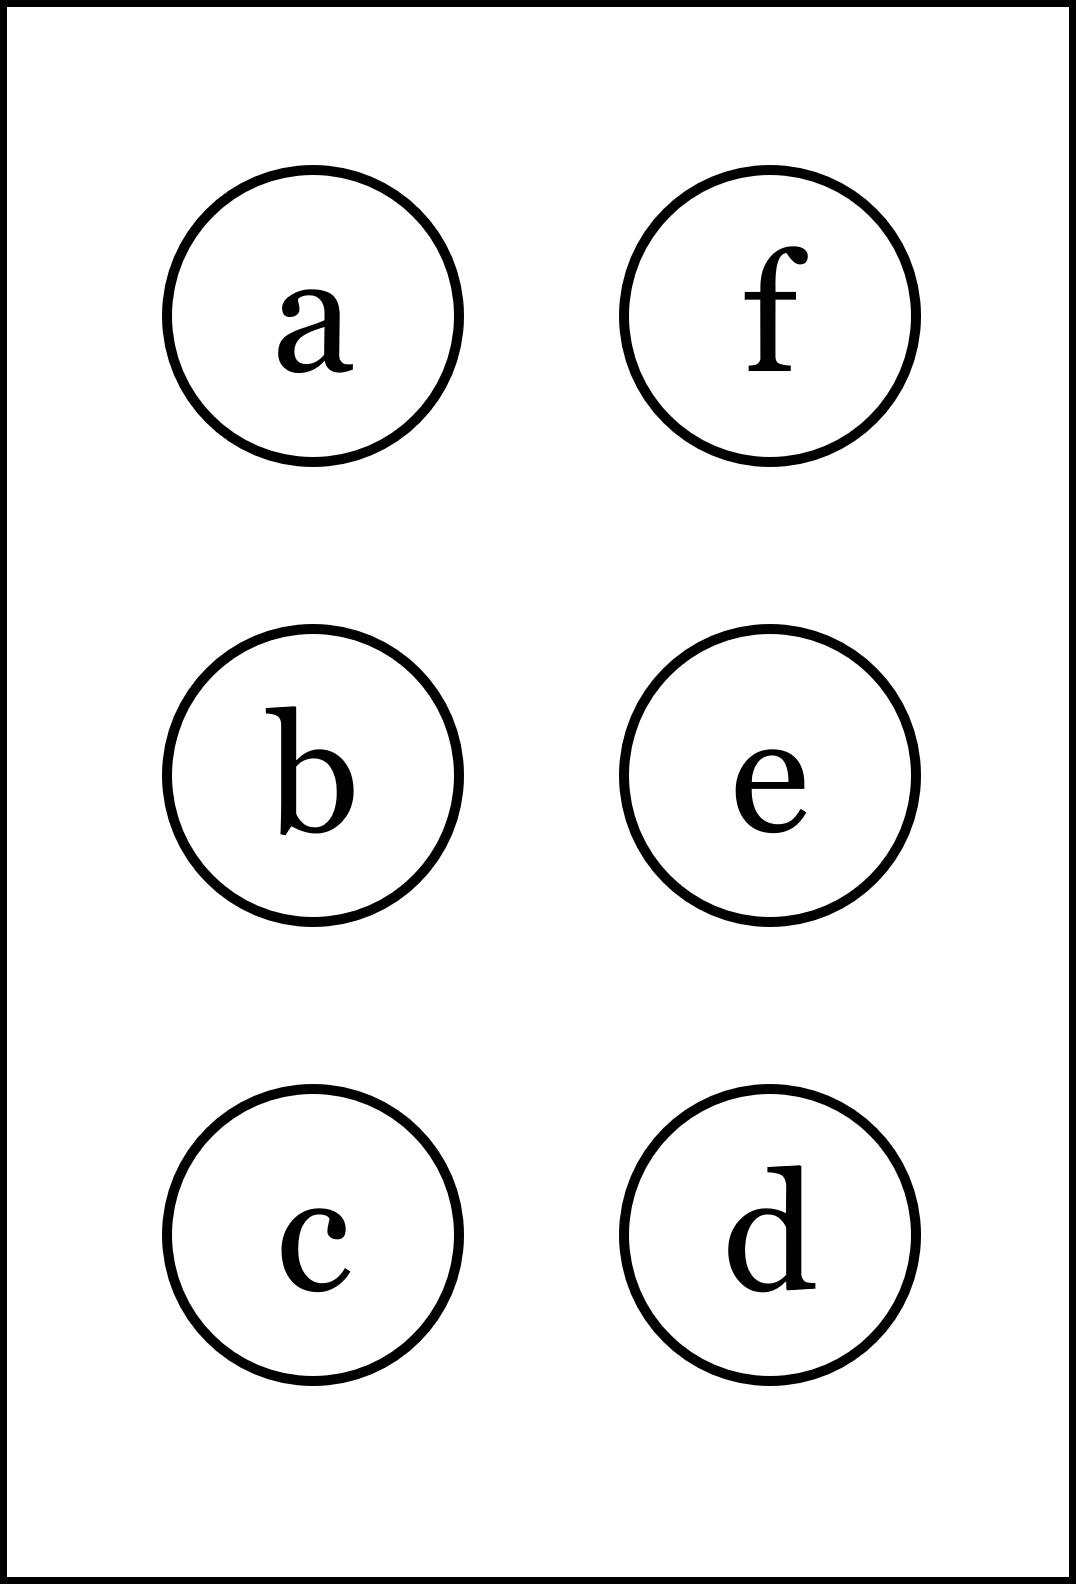
\includegraphics[height=40mm]{../images/braille.png}
{\small Písmeno Braillovej abecedy}
\end{center}
\end{minipage}
\end{center}
\end{minipage}
&
\begin{minipage}[c][104.5mm][t]{0.5\linewidth}
\begin{center}
\vspace{7mm}
{\huge Závorky a zlomky, skupina \textit{Iota $\iota$} -\romannumeral2}\\[5mm]
\textit{Jméno:}\phantom{xxxxxxxxxxxxxxxxxxxxxxxxxxxxxxxxxxxxxxxxxxxxxxxxxxxxxxxxxxxxxxxxx}\\[5mm]
\begin{minipage}{0.95\linewidth}
\begin{center}
\textbf{Uprav výrazy (a) až (f)}. Pokud je výraz za otazníky roven výrazu pred otázniky, tak napravo obarvi príslušející kroužek. \textbf{Spolu odevzdejte výsledné slovo.}
\end{center}
\end{minipage}
\\[1mm]
\begin{minipage}{0.79\linewidth}
\begin{center}
\begin{varwidth}{\linewidth}
\begin{enumerate}
\normalsize
\item $3(-2x+3)-1(4+2x)$\quad \dotfill\; ???\;\dotfill \quad $-8x+5$
\item $2(-2-x)(-9x+1)-2(3-6x)$\quad \dotfill\; ???\;\dotfill \quad $18x^2-46x+10$
\item $(4x-3)^3-(2x+4)^2$\quad \dotfill\; ???\;\dotfill \quad $-64x^3+148x^2-43$
\item $\cfrac{x-2}{2}-3\cfrac{-4+8x}{-6}$\quad \dotfill\; ???\;\dotfill \quad $\cfrac{36}{12}$
\item $\cfrac{\frac{6}{-1}-\frac{4}{x}}{\frac{1}{5}+\frac{3}{-2}}$\quad \dotfill\; ???\;\dotfill \quad $\cfrac{-58x-42}{-13x}$
\item $\cfrac{(-2-7x)^2-1}{(-7x-2)\cdot\frac{2}{x}}$\quad \dotfill\; ???\;\dotfill \quad $\cfrac{49x^3+28x^2-3x}{14x-4}$
\end{enumerate}
\end{varwidth}
\end{center}
\end{minipage}
\begin{minipage}{0.20\linewidth}
\begin{center}
{\Huge\bfseries 2.} \\[2mm]
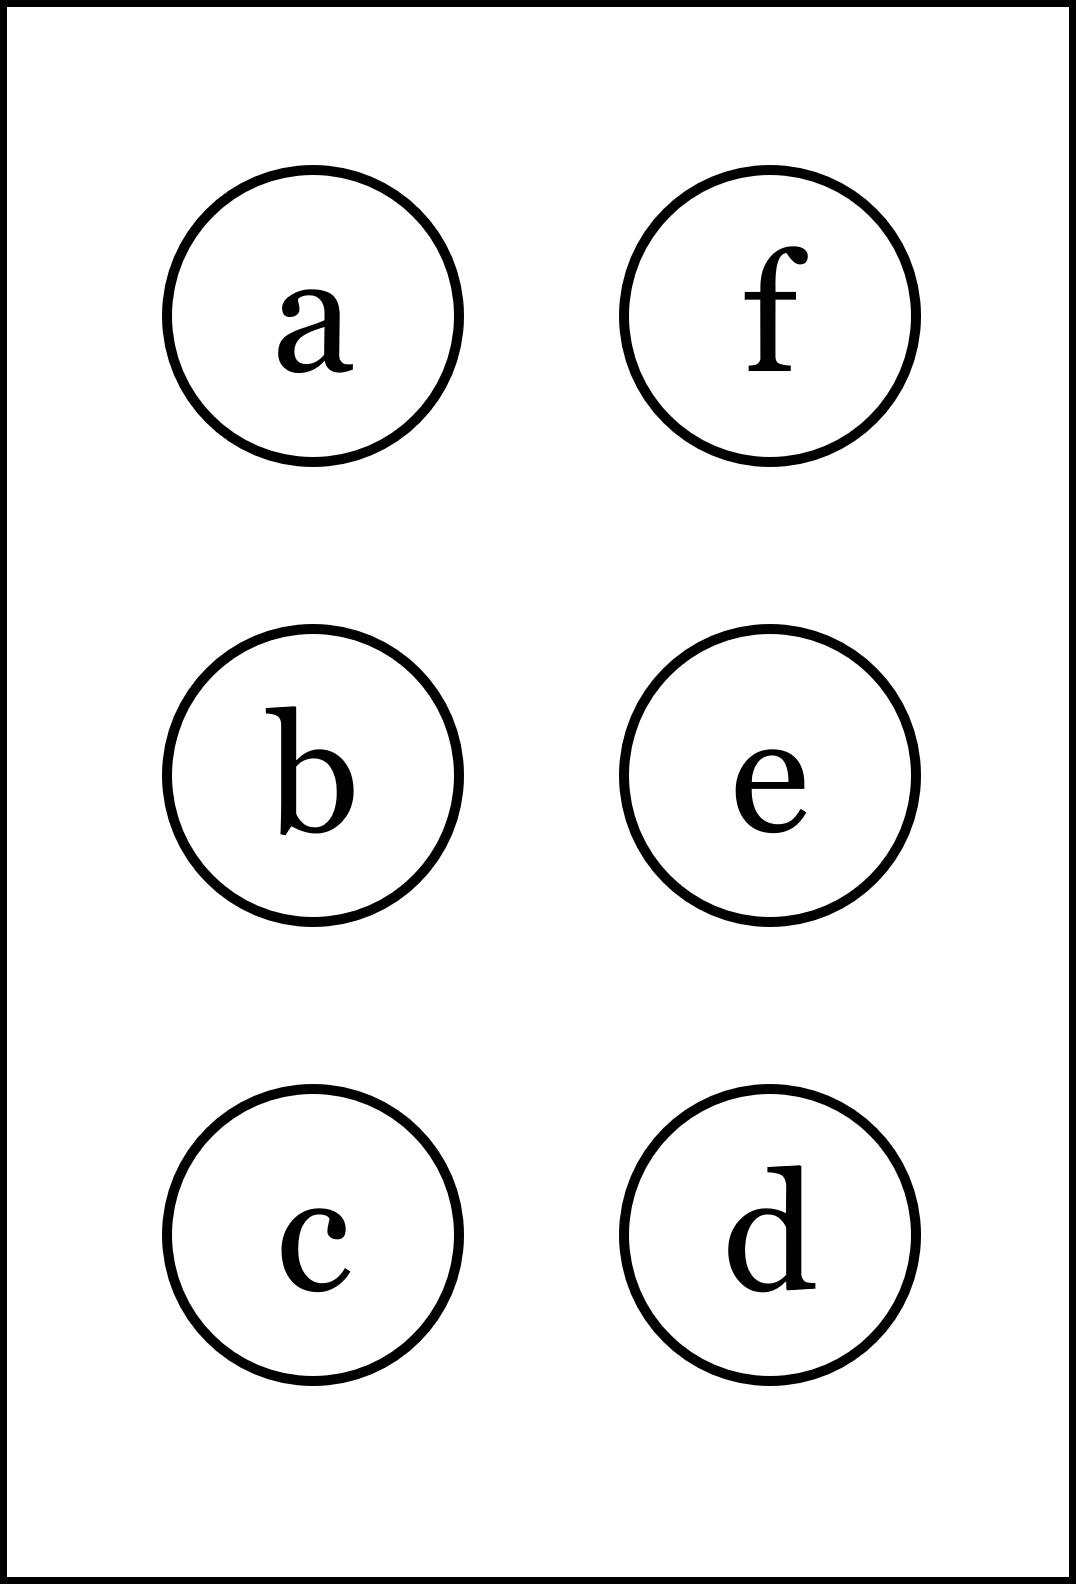
\includegraphics[height=40mm]{../images/braille.png}
{\small Písmeno Braillovej abecedy}
\end{center}
\end{minipage}
\end{center}
\end{minipage}
\\ \hdashline
\begin{minipage}[c][104.5mm][t]{0.5\linewidth}
\begin{center}
\vspace{7mm}
{\huge Závorky a zlomky, skupina \textit{Iota $\iota$} -\romannumeral3}\\[5mm]
\textit{Jméno:}\phantom{xxxxxxxxxxxxxxxxxxxxxxxxxxxxxxxxxxxxxxxxxxxxxxxxxxxxxxxxxxxxxxxxx}\\[5mm]
\begin{minipage}{0.95\linewidth}
\begin{center}
\textbf{Uprav výrazy (a) až (f)}. Pokud je výraz za otazníky roven výrazu pred otázniky, tak napravo obarvi príslušející kroužek. \textbf{Spolu odevzdejte výsledné slovo.}
\end{center}
\end{minipage}
\\[1mm]
\begin{minipage}{0.79\linewidth}
\begin{center}
\begin{varwidth}{\linewidth}
\begin{enumerate}
\normalsize
\item $-7(-4x-3)-2(8+x)$\quad \dotfill\; ???\;\dotfill \quad $26x+5$
\item $4(1-3x)(-x+5)-4(-8-x)$\quad \dotfill\; ???\;\dotfill \quad $12x^2+60x$
\item $(3x-1)^3-(-2x-2)^2$\quad \dotfill\; ???\;\dotfill \quad $27x^3-31x^2+x-5$
\item $\cfrac{-5x+7}{-6}-2\cfrac{3-2x}{2}$\quad \dotfill\; ???\;\dotfill \quad $\cfrac{-34x+50}{12}$
\item $\cfrac{\frac{-6}{-7}-\frac{-3}{x}}{\frac{1}{1}+\frac{-9}{-4}}$\quad \dotfill\; ???\;\dotfill \quad $\cfrac{24x+84}{91x}$
\item $\cfrac{(-2+7x)^2+1}{(2x-2)\cdot\frac{-6}{x}}$\quad \dotfill\; ???\;\dotfill \quad $\cfrac{49x^3-28x^2+5x}{-12x+12}$
\end{enumerate}
\end{varwidth}
\end{center}
\end{minipage}
\begin{minipage}{0.20\linewidth}
\begin{center}
{\Huge\bfseries 3.} \\[2mm]
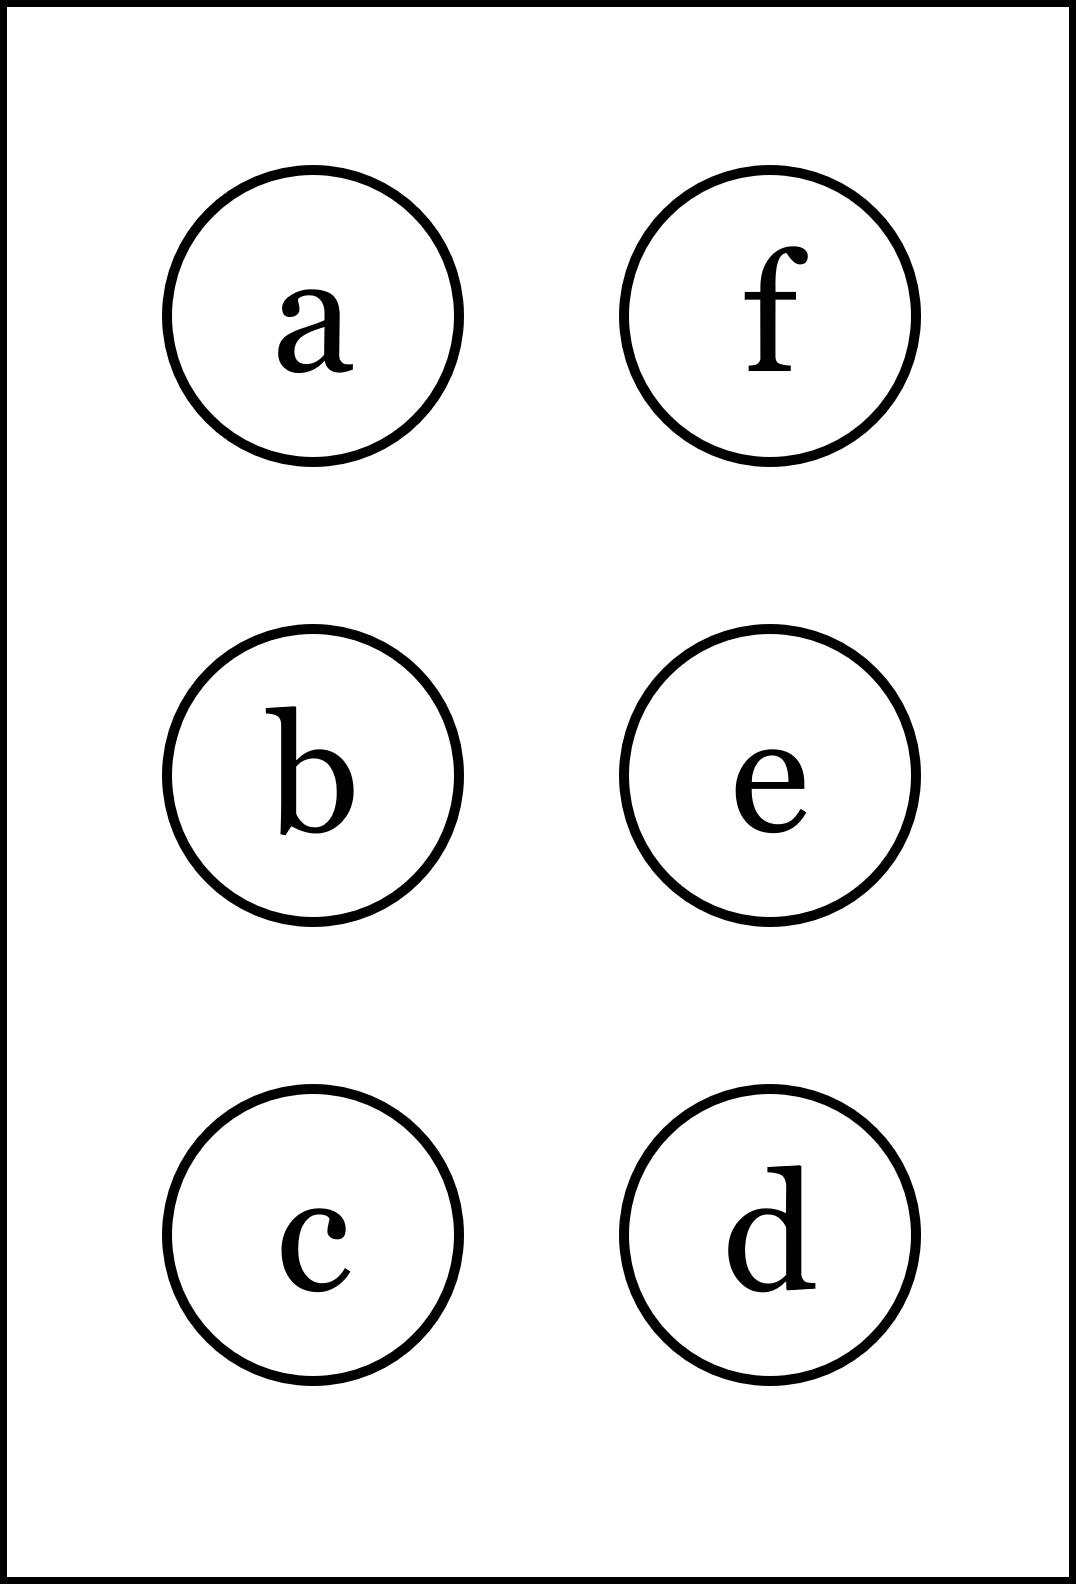
\includegraphics[height=40mm]{../images/braille.png}
{\small Písmeno Braillovej abecedy}
\end{center}
\end{minipage}
\end{center}
\end{minipage}
&
\begin{minipage}[c][104.5mm][t]{0.5\linewidth}
\begin{center}
\vspace{7mm}
{\huge Závorky a zlomky, skupina \textit{Iota $\iota$} -\romannumeral4}\\[5mm]
\textit{Jméno:}\phantom{xxxxxxxxxxxxxxxxxxxxxxxxxxxxxxxxxxxxxxxxxxxxxxxxxxxxxxxxxxxxxxxxx}\\[5mm]
\begin{minipage}{0.95\linewidth}
\begin{center}
\textbf{Uprav výrazy (a) až (f)}. Pokud je výraz za otazníky roven výrazu pred otázniky, tak napravo obarvi príslušející kroužek. \textbf{Spolu odevzdejte výsledné slovo.}
\end{center}
\end{minipage}
\\[1mm]
\begin{minipage}{0.79\linewidth}
\begin{center}
\begin{varwidth}{\linewidth}
\begin{enumerate}
\normalsize
\item $7(-x+4)-5(-8-5x)$\quad \dotfill\; ???\;\dotfill \quad $18x+68$
\item $3(-4+x)(x-3)+3(1-8x)$\quad \dotfill\; ???\;\dotfill \quad $3x^2+45x$
\item $(2x+1)^3-(6x-2)^2$\quad \dotfill\; ???\;\dotfill \quad $-8x^3-24x^2-3$
\item $\cfrac{-4x+3}{2}-2\cfrac{-3-2x}{4}$\quad \dotfill\; ???\;\dotfill \quad $\cfrac{24}{-8}$
\item $\cfrac{\frac{2}{2}-\frac{-8}{x}}{\frac{1}{-1}+\frac{7}{-4}}$\quad \dotfill\; ???\;\dotfill \quad $\cfrac{5x+63}{-22x}$
\item $\cfrac{(1-4x)^2-1}{(3x-3)\cdot\frac{7}{x}}$\quad \dotfill\; ???\;\dotfill \quad $\cfrac{16x^3-8x^2}{-21x-21}$
\end{enumerate}
\end{varwidth}
\end{center}
\end{minipage}
\begin{minipage}{0.20\linewidth}
\begin{center}
{\Huge\bfseries 4.} \\[2mm]
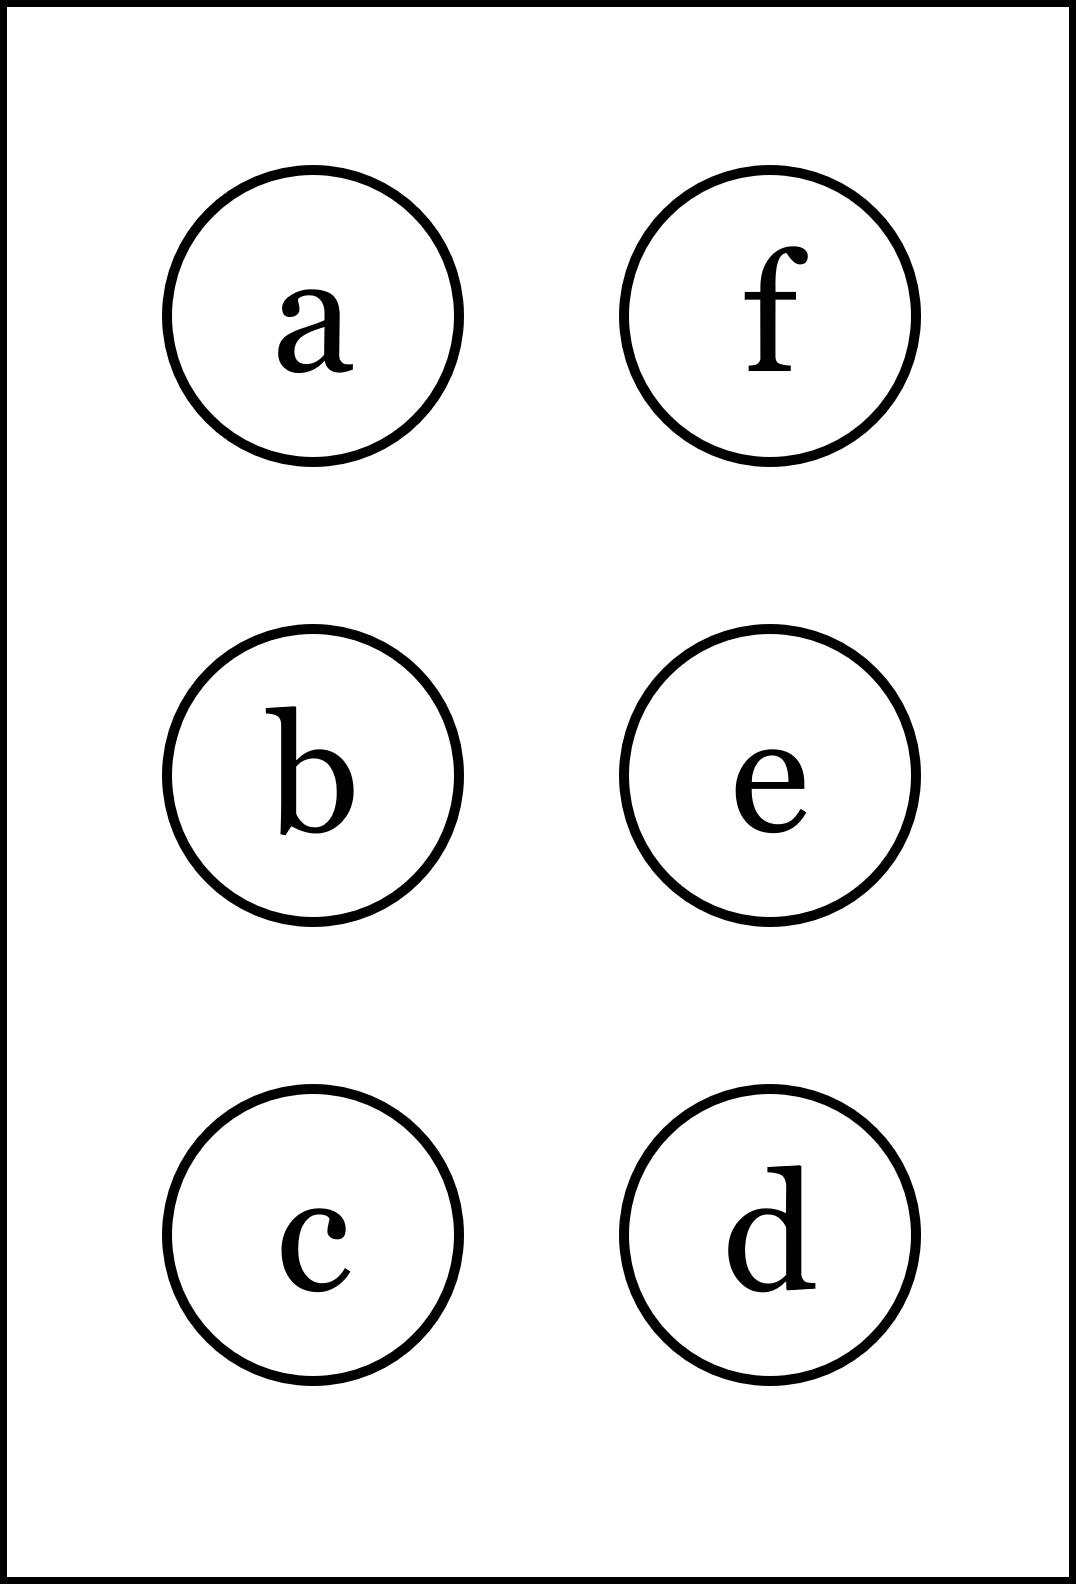
\includegraphics[height=40mm]{../images/braille.png}
{\small Písmeno Braillovej abecedy}
\end{center}
\end{minipage}
\end{center}
\end{minipage}
%
\end{tabular}
\newpage
\thispagestyle{empty}
\begin{tabular}{c:c}
\begin{minipage}[c][104.5mm][t]{0.5\linewidth}
\begin{center}
\vspace{7mm}
{\huge Závorky a zlomky, skupina \textit{Kappa $\kappa$} -\romannumeral1}\\[5mm]
\textit{Jméno:}\phantom{xxxxxxxxxxxxxxxxxxxxxxxxxxxxxxxxxxxxxxxxxxxxxxxxxxxxxxxxxxxxxxxxx}\\[5mm]
\begin{minipage}{0.95\linewidth}
\begin{center}
\textbf{Uprav výrazy (a) až (f)}. Pokud je výraz za otazníky roven výrazu pred otázniky, tak napravo obarvi príslušející kroužek. \textbf{Spolu odevzdejte výsledné slovo.}
\end{center}
\end{minipage}
\\[1mm]
\begin{minipage}{0.79\linewidth}
\begin{center}
\begin{varwidth}{\linewidth}
\begin{enumerate}
\normalsize
\item $-7(3x-4)-1(4-x)$\quad \dotfill\; ???\;\dotfill \quad $-20x+24$
\item $-4(-9+4x)(x+1)-5(-4+5x)$\quad \dotfill\; ???\;\dotfill \quad $-16x^2+5x$
\item $(-x-3)^3-(7x-2)^2$\quad \dotfill\; ???\;\dotfill \quad $x^3+58x^2-31$
\item $\cfrac{-3x-2}{4}+7\cfrac{2+x}{-2}$\quad \dotfill\; ???\;\dotfill \quad $\cfrac{34x+60}{8}$
\item $\cfrac{\frac{3}{3}-\frac{-1}{x}}{\frac{1}{-5}+\frac{-6}{-6}}$\quad \dotfill\; ???\;\dotfill \quad $\cfrac{88x+92}{72x}$
\item $\cfrac{(-2-2x)^2+1}{(-5x-8)\cdot\frac{1}{x}}$\quad \dotfill\; ???\;\dotfill \quad $\cfrac{4x^3+8x^2+5x}{-5x-8}$
\end{enumerate}
\end{varwidth}
\end{center}
\end{minipage}
\begin{minipage}{0.20\linewidth}
\begin{center}
{\Huge\bfseries 1.} \\[2mm]
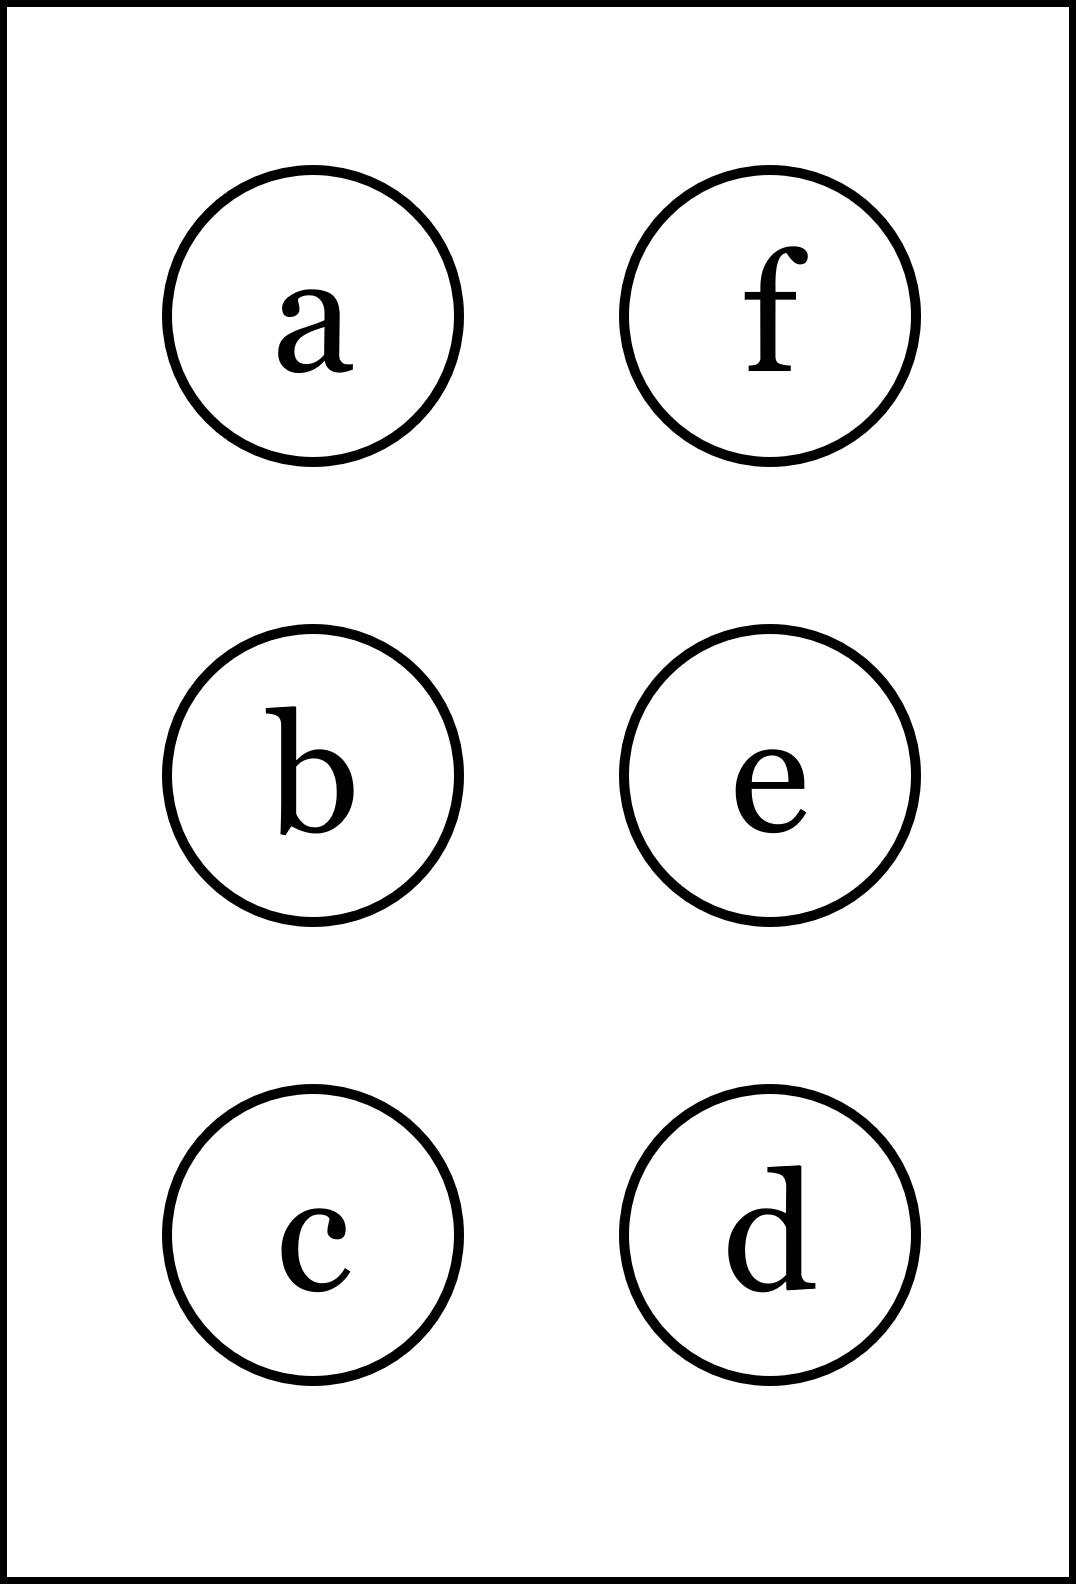
\includegraphics[height=40mm]{../images/braille.png}
{\small Písmeno Braillovej abecedy}
\end{center}
\end{minipage}
\end{center}
\end{minipage}
&
\begin{minipage}[c][104.5mm][t]{0.5\linewidth}
\begin{center}
\vspace{7mm}
{\huge Závorky a zlomky, skupina \textit{Kappa $\kappa$} -\romannumeral2}\\[5mm]
\textit{Jméno:}\phantom{xxxxxxxxxxxxxxxxxxxxxxxxxxxxxxxxxxxxxxxxxxxxxxxxxxxxxxxxxxxxxxxxx}\\[5mm]
\begin{minipage}{0.95\linewidth}
\begin{center}
\textbf{Uprav výrazy (a) až (f)}. Pokud je výraz za otazníky roven výrazu pred otázniky, tak napravo obarvi príslušející kroužek. \textbf{Spolu odevzdejte výsledné slovo.}
\end{center}
\end{minipage}
\\[1mm]
\begin{minipage}{0.79\linewidth}
\begin{center}
\begin{varwidth}{\linewidth}
\begin{enumerate}
\normalsize
\item $6(9x+2)+8(-3+x)$\quad \dotfill\; ???\;\dotfill \quad $62x-12$
\item $-4(1-x)(-4x+2)-9(1-x)$\quad \dotfill\; ???\;\dotfill \quad $-16x^2-33x-17$
\item $(-4x+4)^3-(7x-9)^2$\quad \dotfill\; ???\;\dotfill \quad $-64x^3+143x^2-66x-17$
\item $\cfrac{x-1}{4}+3\cfrac{-8-7x}{8}$\quad \dotfill\; ???\;\dotfill \quad $\cfrac{-76x-104}{32}$
\item $\cfrac{\frac{7}{2}-\frac{3}{x}}{\frac{1}{5}+\frac{5}{2}}$\quad \dotfill\; ???\;\dotfill \quad $\cfrac{69x-58}{54x}$
\item $\cfrac{(-7-8x)^2+7}{(5x+3)\cdot\frac{-1}{x}}$\quad \dotfill\; ???\;\dotfill \quad $\cfrac{64x^3+112x^2-56x}{5x-3}$
\end{enumerate}
\end{varwidth}
\end{center}
\end{minipage}
\begin{minipage}{0.20\linewidth}
\begin{center}
{\Huge\bfseries 2.} \\[2mm]
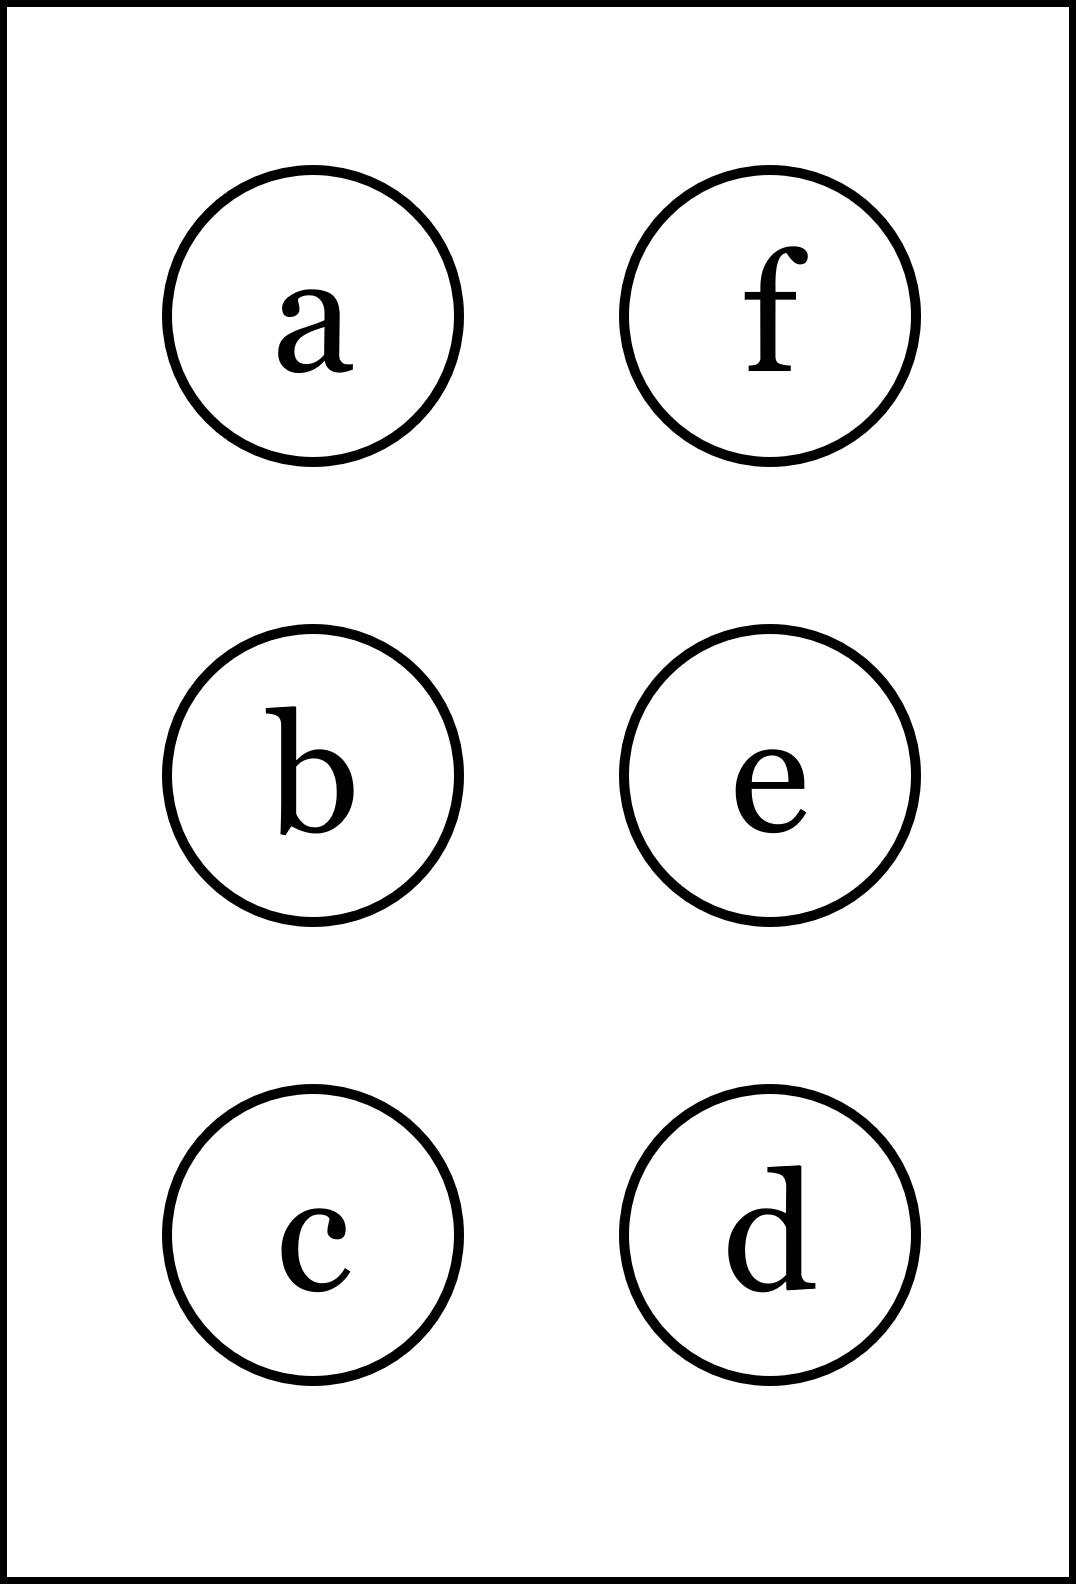
\includegraphics[height=40mm]{../images/braille.png}
{\small Písmeno Braillovej abecedy}
\end{center}
\end{minipage}
\end{center}
\end{minipage}
\\ \hdashline
\begin{minipage}[c][104.5mm][t]{0.5\linewidth}
\begin{center}
\vspace{7mm}
{\huge Závorky a zlomky, skupina \textit{Kappa $\kappa$} -\romannumeral3}\\[5mm]
\textit{Jméno:}\phantom{xxxxxxxxxxxxxxxxxxxxxxxxxxxxxxxxxxxxxxxxxxxxxxxxxxxxxxxxxxxxxxxxx}\\[5mm]
\begin{minipage}{0.95\linewidth}
\begin{center}
\textbf{Uprav výrazy (a) až (f)}. Pokud je výraz za otazníky roven výrazu pred otázniky, tak napravo obarvi príslušející kroužek. \textbf{Spolu odevzdejte výsledné slovo.}
\end{center}
\end{minipage}
\\[1mm]
\begin{minipage}{0.79\linewidth}
\begin{center}
\begin{varwidth}{\linewidth}
\begin{enumerate}
\normalsize
\item $2(-4x-2)+9(3-3x)$\quad \dotfill\; ???\;\dotfill \quad $-35x+23$
\item $4(-3+x)(8x+3)-4(-7-5x)$\quad \dotfill\; ???\;\dotfill \quad $32x^2+64x+8$
\item $(-2x-4)^3-(-3x+3)^2$\quad \dotfill\; ???\;\dotfill \quad $-8x^3-57x^2-78x-73$
\item $\cfrac{x+2}{-2}+8\cfrac{3-3x}{-3}$\quad \dotfill\; ???\;\dotfill \quad $\cfrac{45x-54}{-6}$
\item $\cfrac{\frac{-5}{1}-\frac{6}{x}}{\frac{1}{1}+\frac{2}{-9}}$\quad \dotfill\; ???\;\dotfill \quad $\cfrac{43x+57}{-7x}$
\item $\cfrac{(1+4x)^2+3}{(-4x+7)\cdot\frac{2}{x}}$\quad \dotfill\; ???\;\dotfill \quad $\cfrac{16x^3+8x^2-4x}{8x+14}$
\end{enumerate}
\end{varwidth}
\end{center}
\end{minipage}
\begin{minipage}{0.20\linewidth}
\begin{center}
{\Huge\bfseries 3.} \\[2mm]
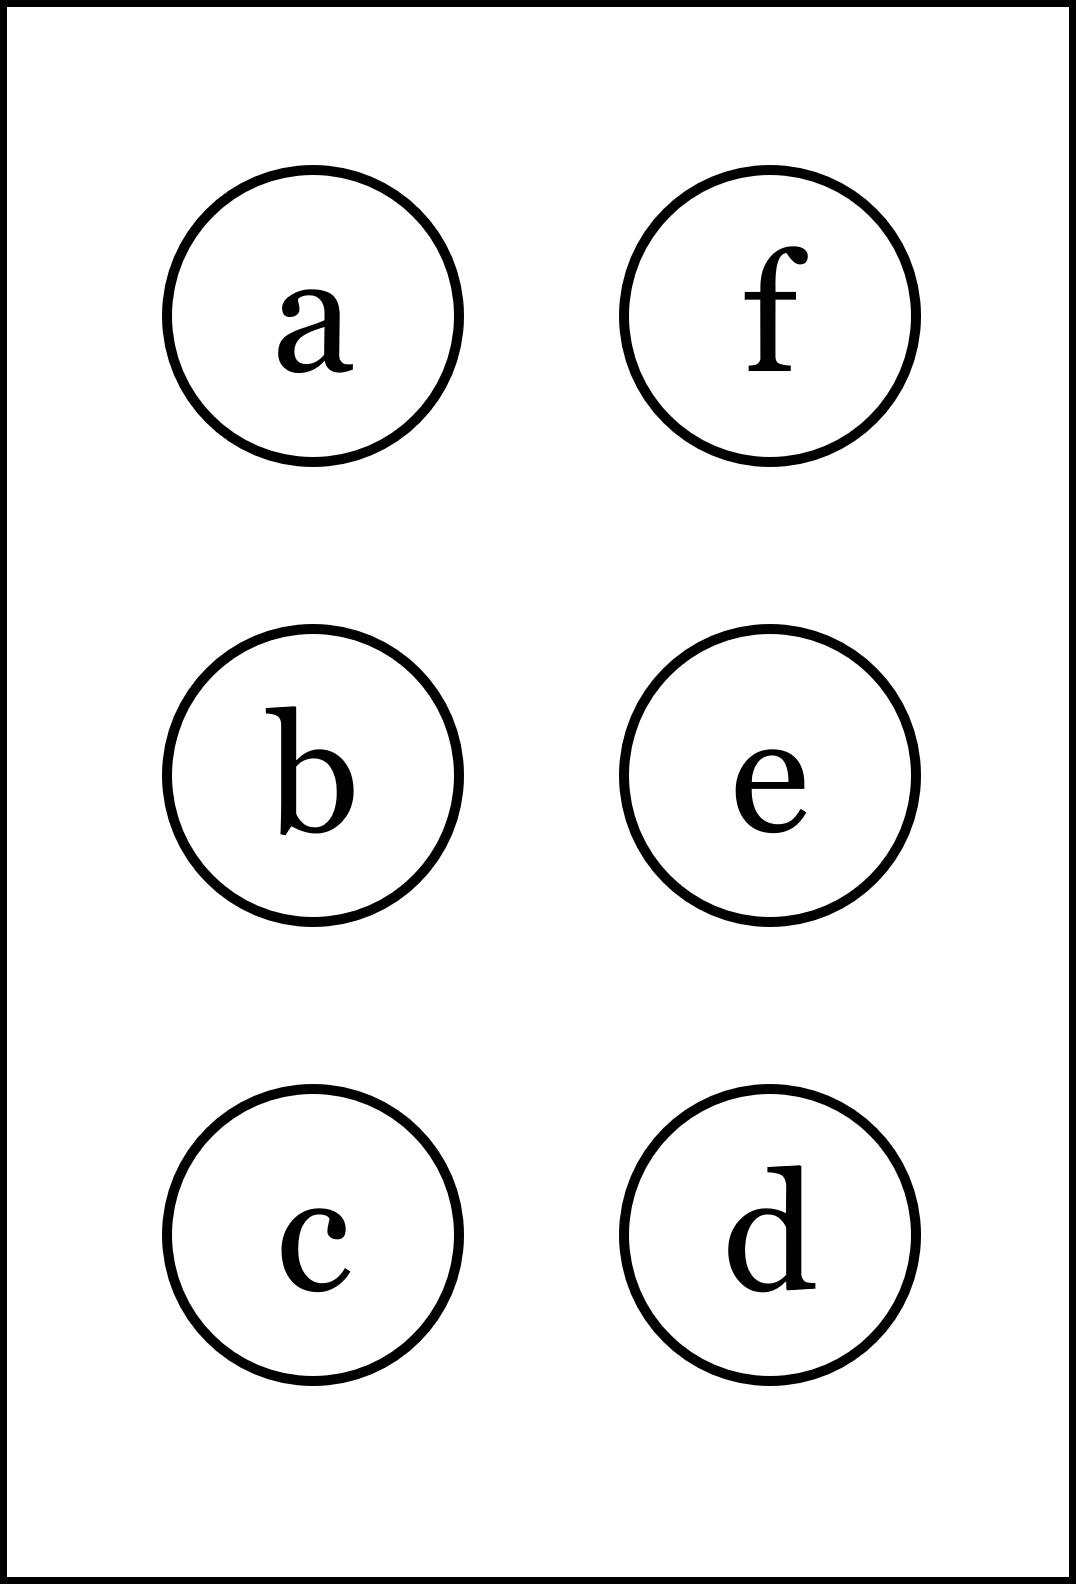
\includegraphics[height=40mm]{../images/braille.png}
{\small Písmeno Braillovej abecedy}
\end{center}
\end{minipage}
\end{center}
\end{minipage}
&
\begin{minipage}[c][104.5mm][t]{0.5\linewidth}
\begin{center}
\vspace{7mm}
{\huge Závorky a zlomky, skupina \textit{Kappa $\kappa$} -\romannumeral4}\\[5mm]
\textit{Jméno:}\phantom{xxxxxxxxxxxxxxxxxxxxxxxxxxxxxxxxxxxxxxxxxxxxxxxxxxxxxxxxxxxxxxxxx}\\[5mm]
\begin{minipage}{0.95\linewidth}
\begin{center}
\textbf{Uprav výrazy (a) až (f)}. Pokud je výraz za otazníky roven výrazu pred otázniky, tak napravo obarvi príslušející kroužek. \textbf{Spolu odevzdejte výsledné slovo.}
\end{center}
\end{minipage}
\\[1mm]
\begin{minipage}{0.79\linewidth}
\begin{center}
\begin{varwidth}{\linewidth}
\begin{enumerate}
\normalsize
\item $2(-2x-4)-4(3+2x)$\quad \dotfill\; ???\;\dotfill \quad $-12x-20$
\item $-2(-3+2x)(7x-4)-3(-4+7x)$\quad \dotfill\; ???\;\dotfill \quad $-28x^2+37x-12$
\item $(-3x+2)^3-(-7x-6)^2$\quad \dotfill\; ???\;\dotfill \quad $-27x^3+5x^2-120x-28$
\item $\cfrac{-6x-3}{5}+4\cfrac{5-3x}{2}$\quad \dotfill\; ???\;\dotfill \quad $\cfrac{72x+94}{-10}$
\item $\cfrac{\frac{-5}{-3}-\frac{-5}{x}}{\frac{1}{-2}+\frac{-6}{-1}}$\quad \dotfill\; ???\;\dotfill \quad $\cfrac{-10x-30}{-33x}$
\item $\cfrac{(2-2x)^2+5}{(-4x+2)\cdot\frac{2}{x}}$\quad \dotfill\; ???\;\dotfill \quad $\cfrac{4x^3-8x^2-9x}{8x+4}$
\end{enumerate}
\end{varwidth}
\end{center}
\end{minipage}
\begin{minipage}{0.20\linewidth}
\begin{center}
{\Huge\bfseries 4.} \\[2mm]
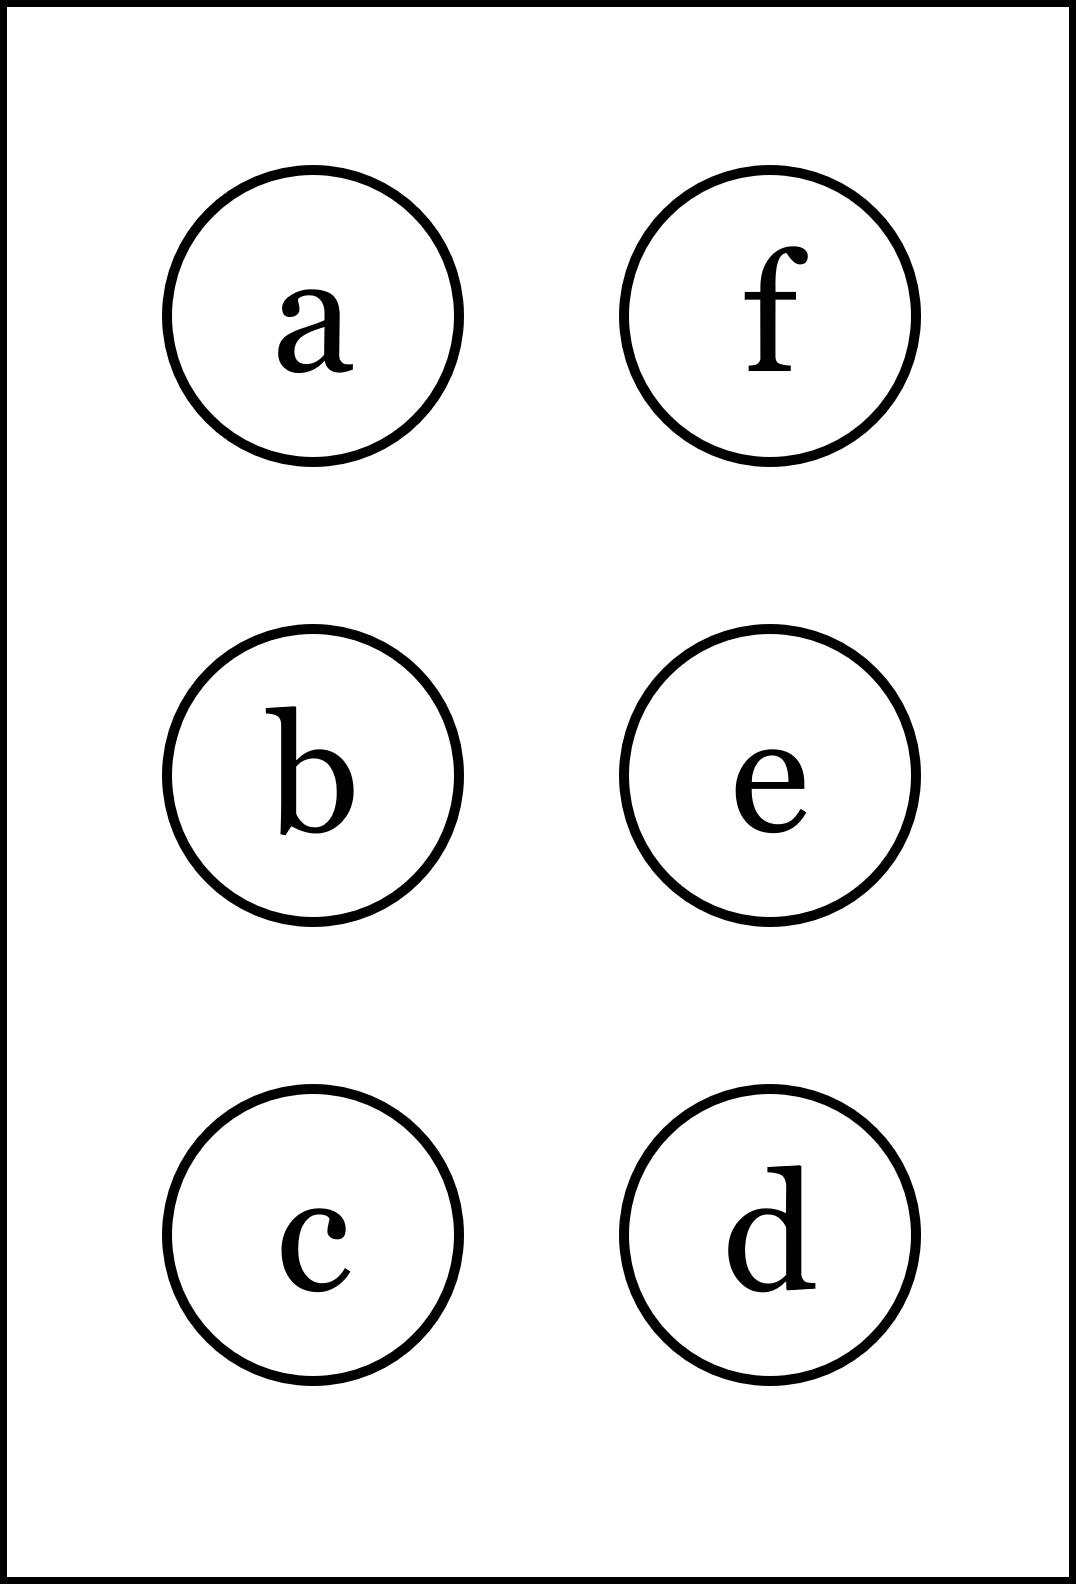
\includegraphics[height=40mm]{../images/braille.png}
{\small Písmeno Braillovej abecedy}
\end{center}
\end{minipage}
\end{center}
\end{minipage}
%
\end{tabular}
\newpage
\thispagestyle{empty}
\begin{tabular}{c:c}
\begin{minipage}[c][104.5mm][t]{0.5\linewidth}
\begin{center}
\vspace{7mm}
{\huge Závorky a zlomky, skupina \textit{Lambda $\lambda$} -\romannumeral1}\\[5mm]
\textit{Jméno:}\phantom{xxxxxxxxxxxxxxxxxxxxxxxxxxxxxxxxxxxxxxxxxxxxxxxxxxxxxxxxxxxxxxxxx}\\[5mm]
\begin{minipage}{0.95\linewidth}
\begin{center}
\textbf{Uprav výrazy (a) až (f)}. Pokud je výraz za otazníky roven výrazu pred otázniky, tak napravo obarvi príslušející kroužek. \textbf{Spolu odevzdejte výsledné slovo.}
\end{center}
\end{minipage}
\\[1mm]
\begin{minipage}{0.79\linewidth}
\begin{center}
\begin{varwidth}{\linewidth}
\begin{enumerate}
\normalsize
\item $5(-7x+1)+8(2+6x)$\quad \dotfill\; ???\;\dotfill \quad $13x$
\item $4(2-x)(3x+2)-4(-5-2x)$\quad \dotfill\; ???\;\dotfill \quad $-12x^2+24x+36$
\item $(-3x-4)^3-(x-4)^2$\quad \dotfill\; ???\;\dotfill \quad $27x^3+109x^2-80$
\item $\cfrac{2x-6}{-6}-3\cfrac{-2-3x}{5}$\quad \dotfill\; ???\;\dotfill \quad $\cfrac{-44x-66}{30}$
\item $\cfrac{\frac{4}{3}-\frac{-1}{x}}{\frac{1}{5}+\frac{-2}{4}}$\quad \dotfill\; ???\;\dotfill \quad $\cfrac{80x+60}{-18x}$
\item $\cfrac{(3-3x)^2-7}{(2x+6)\cdot\frac{-5}{x}}$\quad \dotfill\; ???\;\dotfill \quad $\cfrac{9x^3-18x^2+2x}{-10x-30}$
\end{enumerate}
\end{varwidth}
\end{center}
\end{minipage}
\begin{minipage}{0.20\linewidth}
\begin{center}
{\Huge\bfseries 1.} \\[2mm]
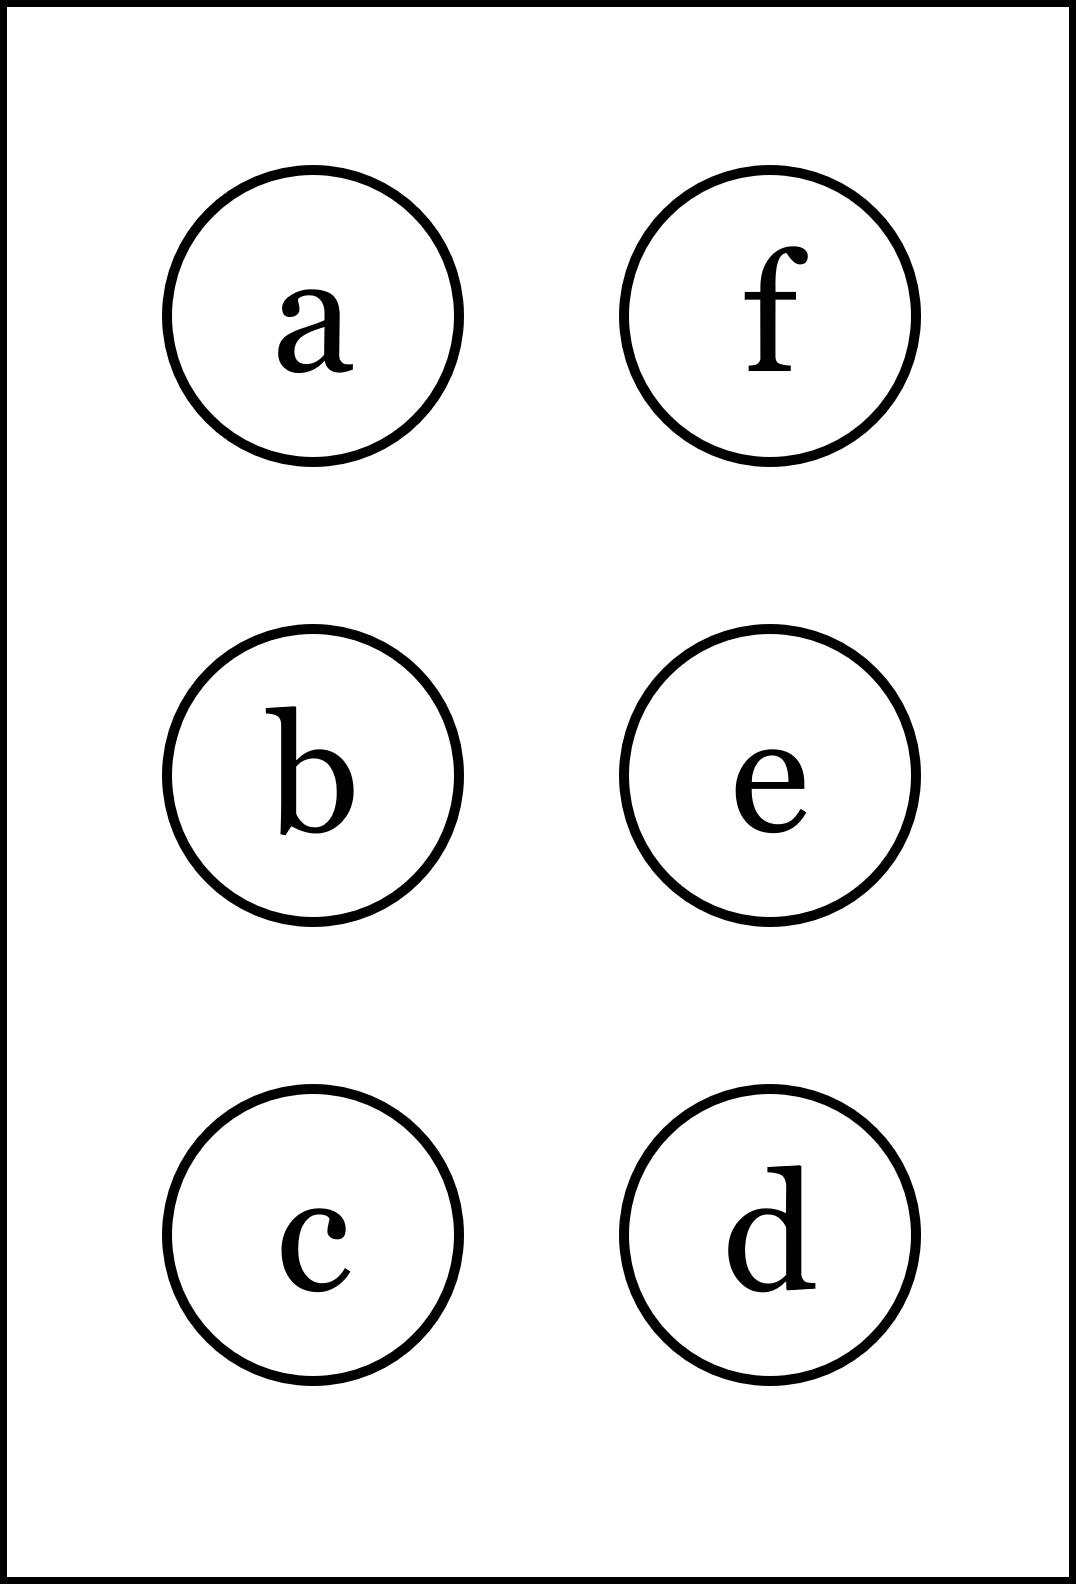
\includegraphics[height=40mm]{../images/braille.png}
{\small Písmeno Braillovej abecedy}
\end{center}
\end{minipage}
\end{center}
\end{minipage}
&
\begin{minipage}[c][104.5mm][t]{0.5\linewidth}
\begin{center}
\vspace{7mm}
{\huge Závorky a zlomky, skupina \textit{Lambda $\lambda$} -\romannumeral2}\\[5mm]
\textit{Jméno:}\phantom{xxxxxxxxxxxxxxxxxxxxxxxxxxxxxxxxxxxxxxxxxxxxxxxxxxxxxxxxxxxxxxxxx}\\[5mm]
\begin{minipage}{0.95\linewidth}
\begin{center}
\textbf{Uprav výrazy (a) až (f)}. Pokud je výraz za otazníky roven výrazu pred otázniky, tak napravo obarvi príslušející kroužek. \textbf{Spolu odevzdejte výsledné slovo.}
\end{center}
\end{minipage}
\\[1mm]
\begin{minipage}{0.79\linewidth}
\begin{center}
\begin{varwidth}{\linewidth}
\begin{enumerate}
\normalsize
\item $-4(7x-4)-6(6-3x)$\quad \dotfill\; ???\;\dotfill \quad $-10x-20$
\item $4(-6+3x)(2x-2)-2(-5+6x)$\quad \dotfill\; ???\;\dotfill \quad $24x^2+84x$
\item $(2x-2)^3-(2x+7)^2$\quad \dotfill\; ???\;\dotfill \quad $-8x^3-28x^2-57$
\item $\cfrac{3x+7}{-7}+3\cfrac{-3+4x}{-4}$\quad \dotfill\; ???\;\dotfill \quad $\cfrac{-96x+35}{-28}$
\item $\cfrac{\frac{-2}{-1}-\frac{-7}{x}}{\frac{1}{-3}+\frac{-7}{-3}}$\quad \dotfill\; ???\;\dotfill \quad $\cfrac{-20x-64}{-18x}$
\item $\cfrac{(-6-7x)^2+7}{(7x-4)\cdot\frac{7}{x}}$\quad \dotfill\; ???\;\dotfill \quad $\cfrac{49x^3+84x^2-43x}{-49x-28}$
\end{enumerate}
\end{varwidth}
\end{center}
\end{minipage}
\begin{minipage}{0.20\linewidth}
\begin{center}
{\Huge\bfseries 2.} \\[2mm]
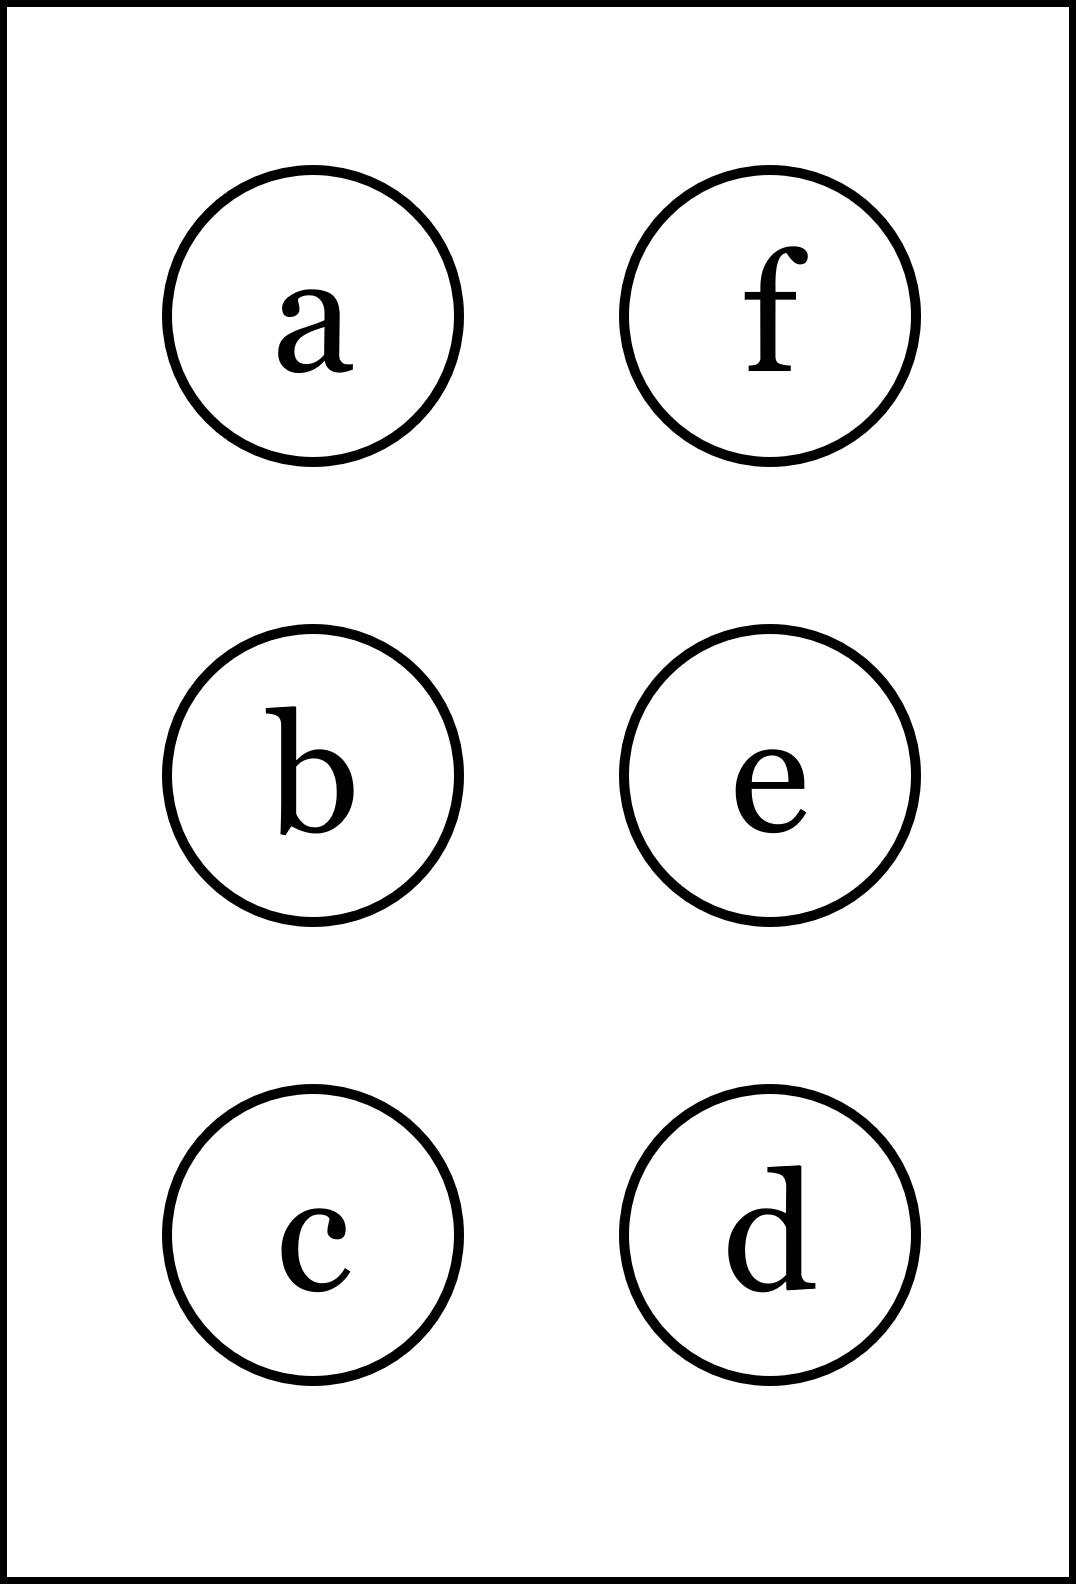
\includegraphics[height=40mm]{../images/braille.png}
{\small Písmeno Braillovej abecedy}
\end{center}
\end{minipage}
\end{center}
\end{minipage}
\\ \hdashline
\begin{minipage}[c][104.5mm][t]{0.5\linewidth}
\begin{center}
\vspace{7mm}
{\huge Závorky a zlomky, skupina \textit{Lambda $\lambda$} -\romannumeral3}\\[5mm]
\textit{Jméno:}\phantom{xxxxxxxxxxxxxxxxxxxxxxxxxxxxxxxxxxxxxxxxxxxxxxxxxxxxxxxxxxxxxxxxx}\\[5mm]
\begin{minipage}{0.95\linewidth}
\begin{center}
\textbf{Uprav výrazy (a) až (f)}. Pokud je výraz za otazníky roven výrazu pred otázniky, tak napravo obarvi príslušející kroužek. \textbf{Spolu odevzdejte výsledné slovo.}
\end{center}
\end{minipage}
\\[1mm]
\begin{minipage}{0.79\linewidth}
\begin{center}
\begin{varwidth}{\linewidth}
\begin{enumerate}
\normalsize
\item $-6(-8x+6)-2(4-x)$\quad \dotfill\; ???\;\dotfill \quad $50x-44$
\item $3(4-3x)(-5x-8)+2(5+x)$\quad \dotfill\; ???\;\dotfill \quad $45x^2+14x-86$
\item $(x+2)^3-(9x+3)^2$\quad \dotfill\; ???\;\dotfill \quad $x^3-75x^2-42x-1$
\item $\cfrac{-4x-5}{-3}-5\cfrac{1-2x}{2}$\quad \dotfill\; ???\;\dotfill \quad $\cfrac{-38x+5}{6}$
\item $\cfrac{\frac{3}{-2}-\frac{-7}{x}}{\frac{1}{-4}+\frac{-1}{1}}$\quad \dotfill\; ???\;\dotfill \quad $\cfrac{-12x+56}{-10x}$
\item $\cfrac{(-4+x)^2+4}{(7x-6)\cdot\frac{-2}{x}}$\quad \dotfill\; ???\;\dotfill \quad $\cfrac{x^3-8x^2-20x}{14x+12}$
\end{enumerate}
\end{varwidth}
\end{center}
\end{minipage}
\begin{minipage}{0.20\linewidth}
\begin{center}
{\Huge\bfseries 3.} \\[2mm]
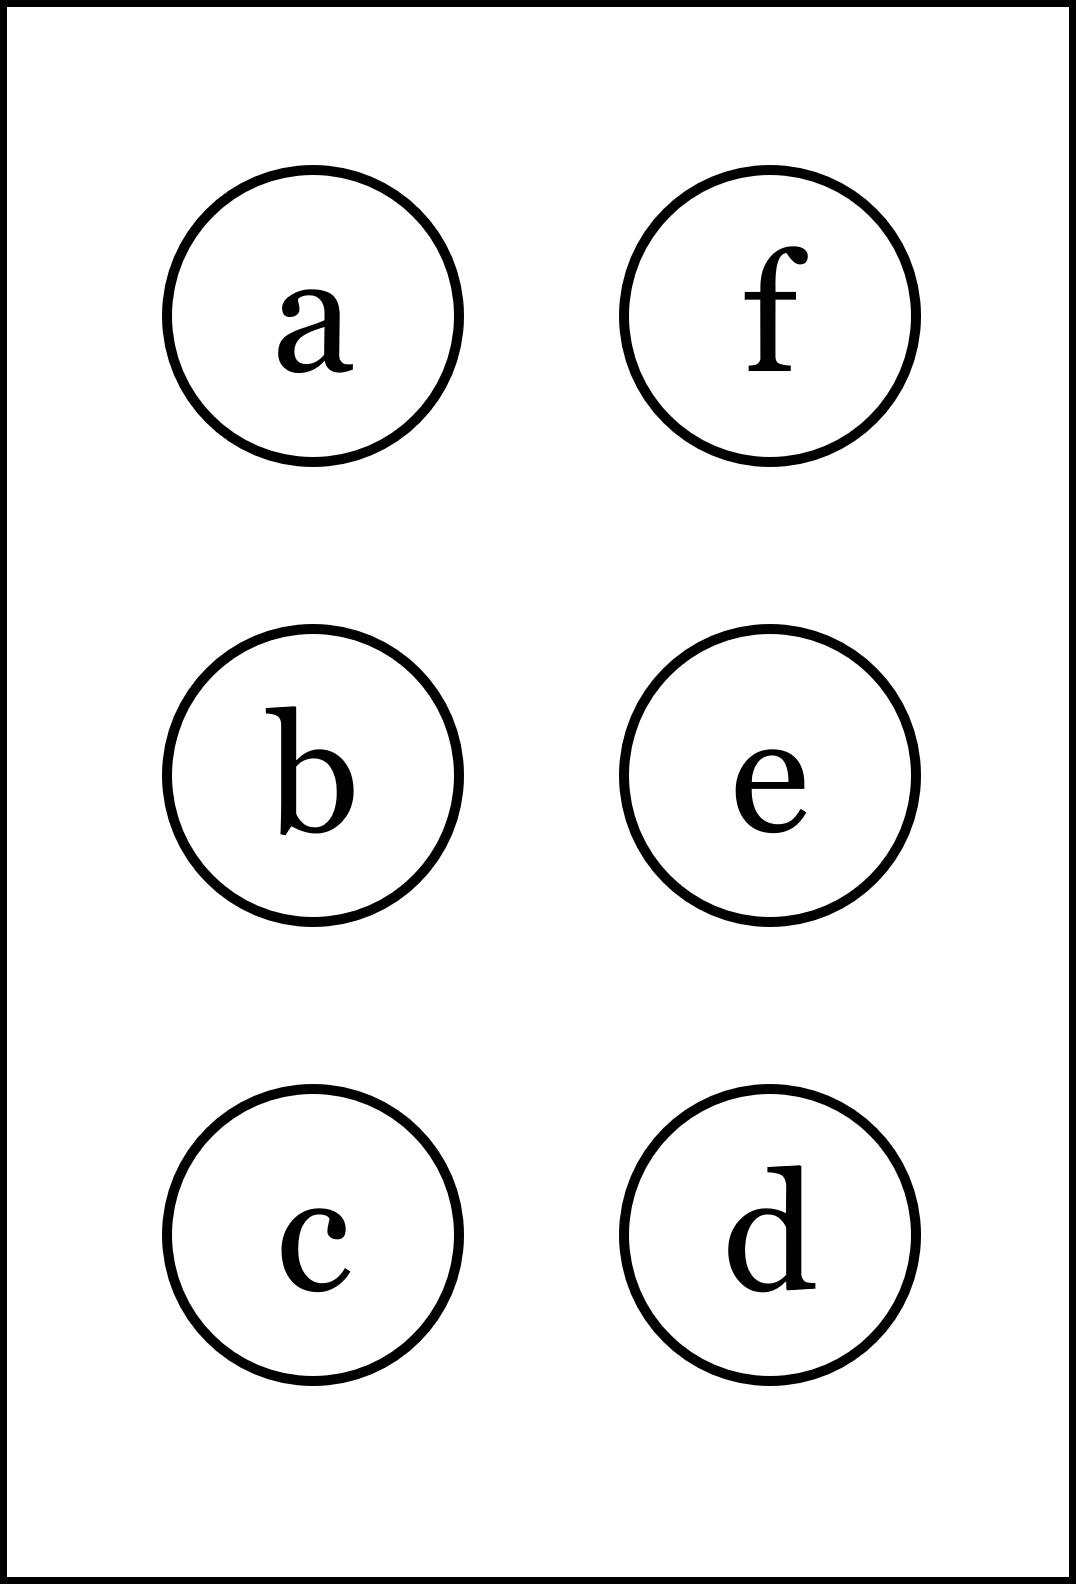
\includegraphics[height=40mm]{../images/braille.png}
{\small Písmeno Braillovej abecedy}
\end{center}
\end{minipage}
\end{center}
\end{minipage}
&
\begin{minipage}[c][104.5mm][t]{0.5\linewidth}
\begin{center}
\vspace{7mm}
{\huge Závorky a zlomky, skupina \textit{Lambda $\lambda$} -\romannumeral4}\\[5mm]
\textit{Jméno:}\phantom{xxxxxxxxxxxxxxxxxxxxxxxxxxxxxxxxxxxxxxxxxxxxxxxxxxxxxxxxxxxxxxxxx}\\[5mm]
\begin{minipage}{0.95\linewidth}
\begin{center}
\textbf{Uprav výrazy (a) až (f)}. Pokud je výraz za otazníky roven výrazu pred otázniky, tak napravo obarvi príslušející kroužek. \textbf{Spolu odevzdejte výsledné slovo.}
\end{center}
\end{minipage}
\\[1mm]
\begin{minipage}{0.79\linewidth}
\begin{center}
\begin{varwidth}{\linewidth}
\begin{enumerate}
\normalsize
\item $2(4x-3)+2(2-9x)$\quad \dotfill\; ???\;\dotfill \quad $-10x-2$
\item $-3(-3-4x)(-8x-7)+2(-9+x)$\quad \dotfill\; ???\;\dotfill \quad $-96x^2+154x+81$
\item $(x+4)^3-(-4x+5)^2$\quad \dotfill\; ???\;\dotfill \quad $x^3-4x^2+88x+39$
\item $\cfrac{6x+5}{-6}-3\cfrac{-1-x}{4}$\quad \dotfill\; ???\;\dotfill \quad $\cfrac{2}{24}$
\item $\cfrac{\frac{-2}{1}-\frac{-1}{x}}{\frac{1}{8}+\frac{1}{-2}}$\quad \dotfill\; ???\;\dotfill \quad $\cfrac{32x-16}{6x}$
\item $\cfrac{(9+3x)^2+6}{(-3x+3)\cdot\frac{2}{x}}$\quad \dotfill\; ???\;\dotfill \quad $\cfrac{9x^3+54x^2-87x}{6x+6}$
\end{enumerate}
\end{varwidth}
\end{center}
\end{minipage}
\begin{minipage}{0.20\linewidth}
\begin{center}
{\Huge\bfseries 4.} \\[2mm]
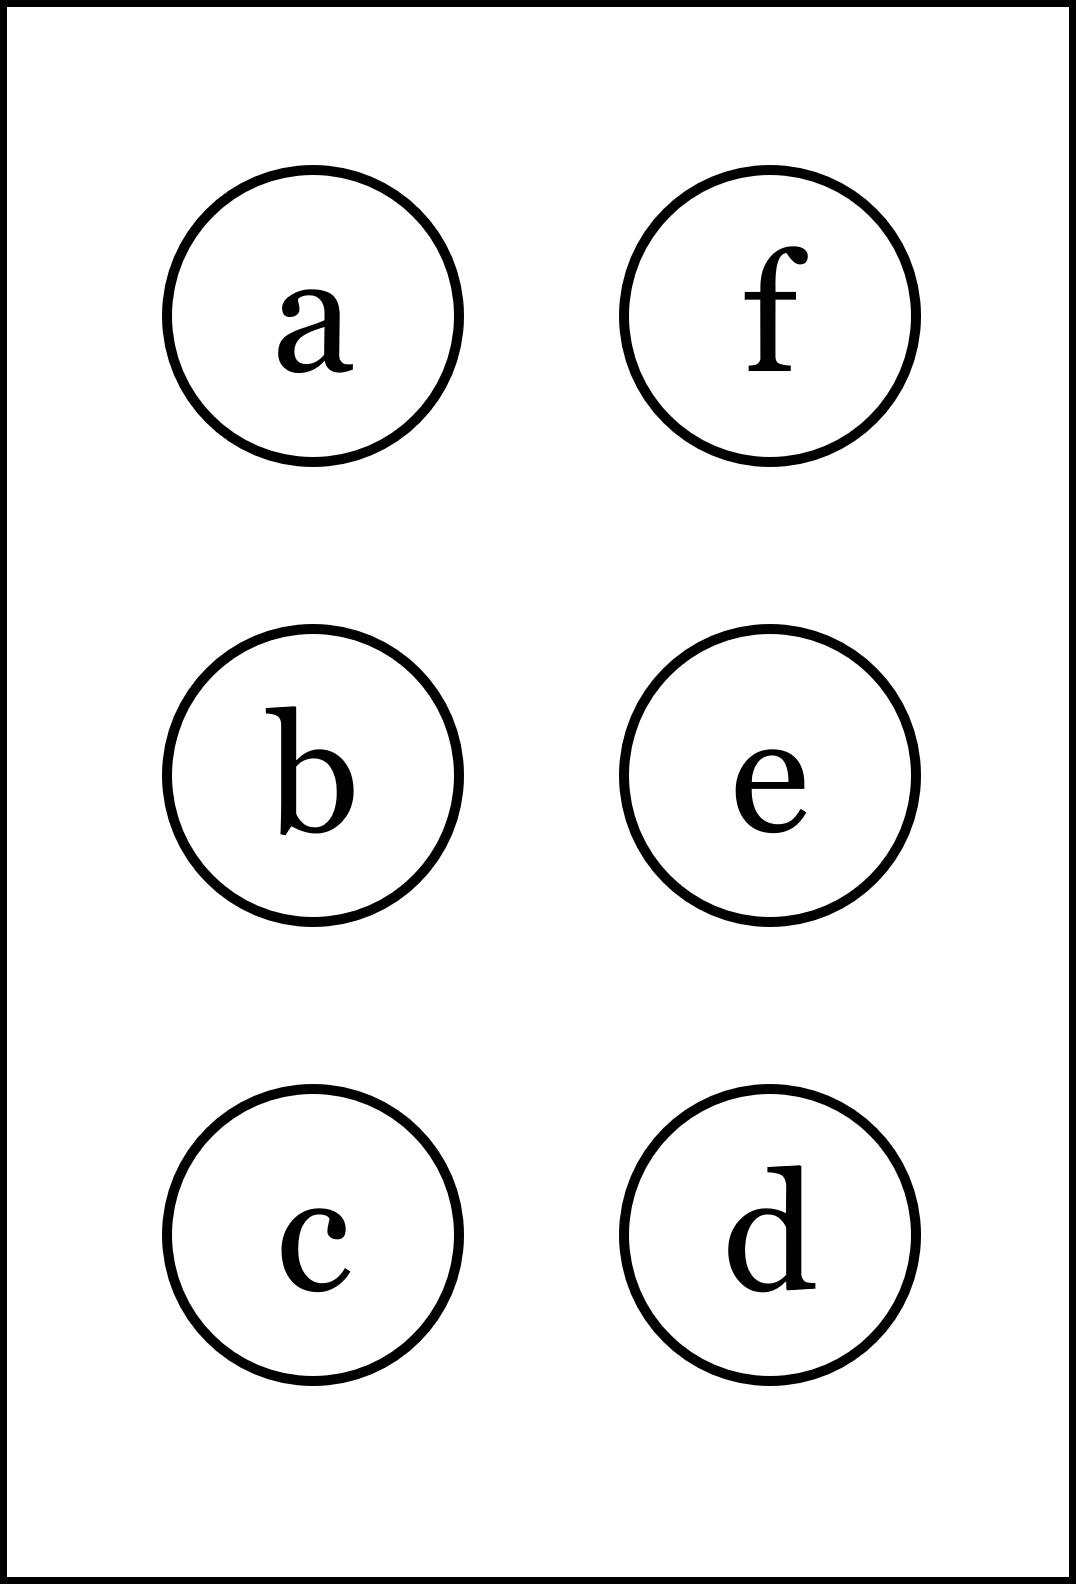
\includegraphics[height=40mm]{../images/braille.png}
{\small Písmeno Braillovej abecedy}
\end{center}
\end{minipage}
\end{center}
\end{minipage}
%
\end{tabular}
\newpage
\thispagestyle{empty}
\begin{tabular}{c:c}
\begin{minipage}[c][104.5mm][t]{0.5\linewidth}
\begin{center}
\vspace{7mm}
{\huge Závorky a zlomky, skupina \textit{Mu $\mu$} -\romannumeral1}\\[5mm]
\textit{Jméno:}\phantom{xxxxxxxxxxxxxxxxxxxxxxxxxxxxxxxxxxxxxxxxxxxxxxxxxxxxxxxxxxxxxxxxx}\\[5mm]
\begin{minipage}{0.95\linewidth}
\begin{center}
\textbf{Uprav výrazy (a) až (f)}. Pokud je výraz za otazníky roven výrazu pred otázniky, tak napravo obarvi príslušející kroužek. \textbf{Spolu odevzdejte výsledné slovo.}
\end{center}
\end{minipage}
\\[1mm]
\begin{minipage}{0.79\linewidth}
\begin{center}
\begin{varwidth}{\linewidth}
\begin{enumerate}
\normalsize
\item $6(3x-3)-1(-1+3x)$\quad \dotfill\; ???\;\dotfill \quad $15x-17$
\item $2(2-8x)(4x-4)+9(5-x)$\quad \dotfill\; ???\;\dotfill \quad $-64x^2-71x+29$
\item $(3x+2)^3-(-6x-6)^2$\quad \dotfill\; ???\;\dotfill \quad $-27x^3+18x^2-36x-28$
\item $\cfrac{5x-1}{4}+7\cfrac{2-x}{-3}$\quad \dotfill\; ???\;\dotfill \quad $\cfrac{59}{12}$
\item $\cfrac{\frac{6}{3}-\frac{1}{x}}{\frac{1}{3}+\frac{5}{-3}}$\quad \dotfill\; ???\;\dotfill \quad $\cfrac{-55x+26}{36x}$
\item $\cfrac{(-4-2x)^2+3}{(-6x+3)\cdot\frac{-1}{x}}$\quad \dotfill\; ???\;\dotfill \quad $\cfrac{4x^3+16x^2+19x}{6x-3}$
\end{enumerate}
\end{varwidth}
\end{center}
\end{minipage}
\begin{minipage}{0.20\linewidth}
\begin{center}
{\Huge\bfseries 1.} \\[2mm]
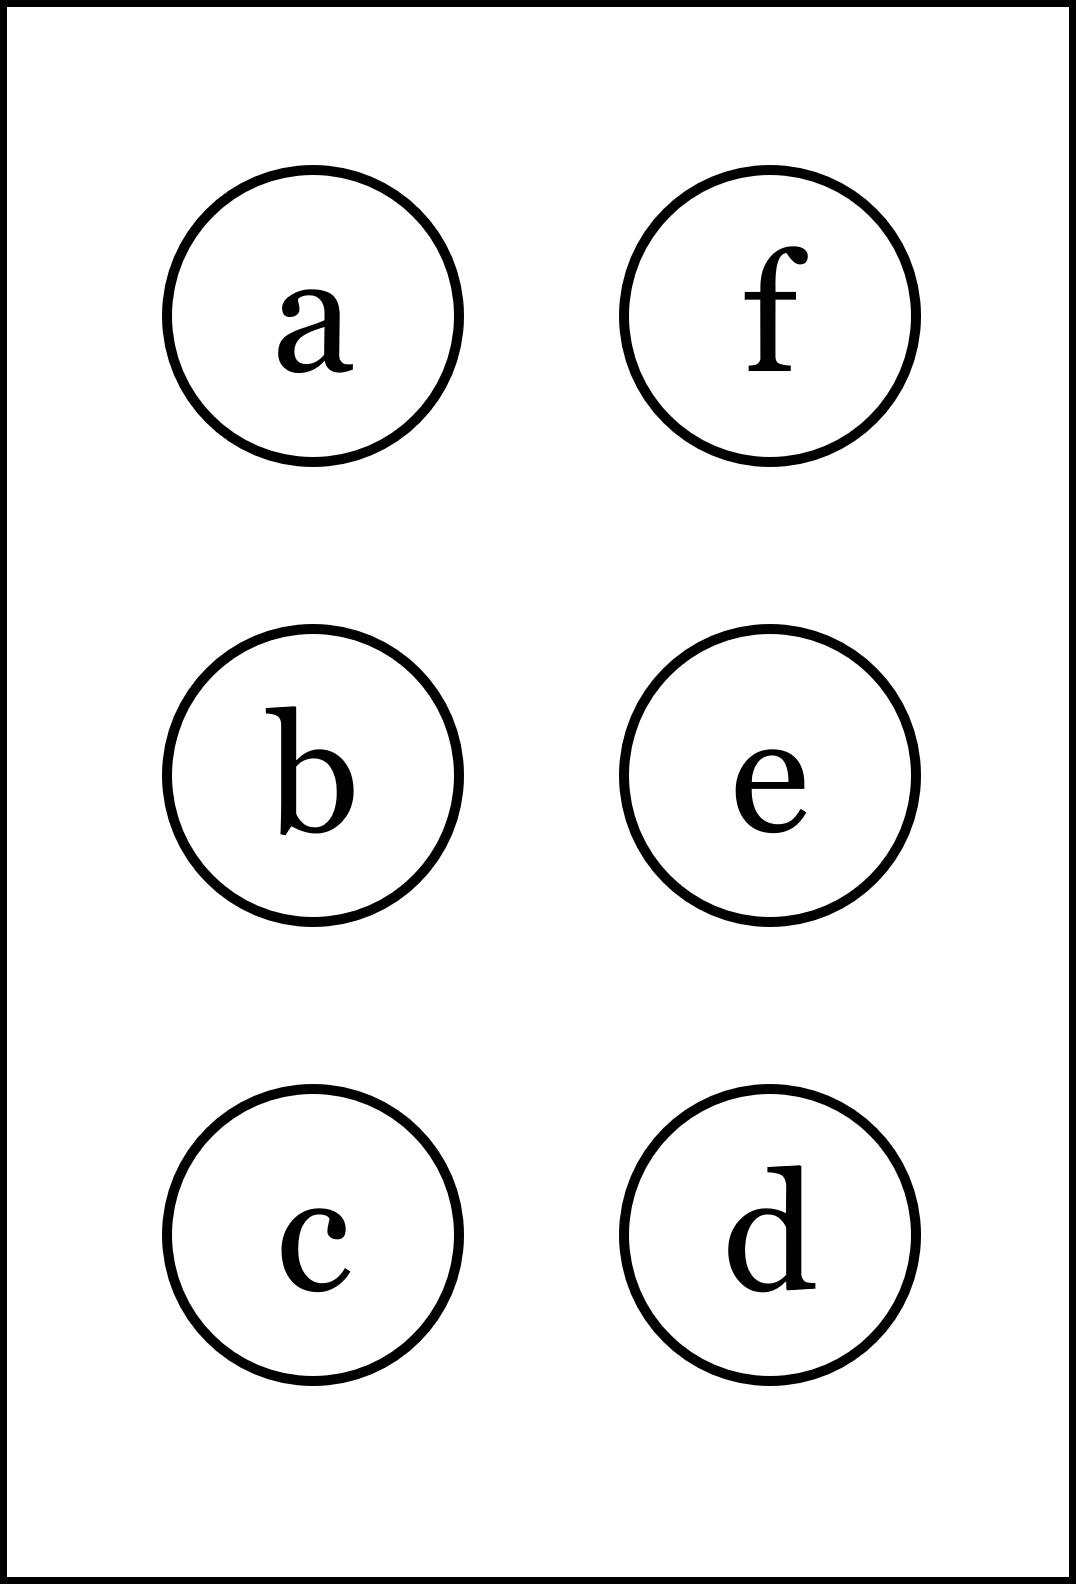
\includegraphics[height=40mm]{../images/braille.png}
{\small Písmeno Braillovej abecedy}
\end{center}
\end{minipage}
\end{center}
\end{minipage}
&
\begin{minipage}[c][104.5mm][t]{0.5\linewidth}
\begin{center}
\vspace{7mm}
{\huge Závorky a zlomky, skupina \textit{Mu $\mu$} -\romannumeral2}\\[5mm]
\textit{Jméno:}\phantom{xxxxxxxxxxxxxxxxxxxxxxxxxxxxxxxxxxxxxxxxxxxxxxxxxxxxxxxxxxxxxxxxx}\\[5mm]
\begin{minipage}{0.95\linewidth}
\begin{center}
\textbf{Uprav výrazy (a) až (f)}. Pokud je výraz za otazníky roven výrazu pred otázniky, tak napravo obarvi príslušející kroužek. \textbf{Spolu odevzdejte výsledné slovo.}
\end{center}
\end{minipage}
\\[1mm]
\begin{minipage}{0.79\linewidth}
\begin{center}
\begin{varwidth}{\linewidth}
\begin{enumerate}
\normalsize
\item $-3(9x+3)-1(-2-x)$\quad \dotfill\; ???\;\dotfill \quad $-26x-7$
\item $-6(4-4x)(2x+3)+1(-7-2x)$\quad \dotfill\; ???\;\dotfill \quad $48x^2-22x-79$
\item $(-4x-2)^3-(8x+4)^2$\quad \dotfill\; ???\;\dotfill \quad $-64x^3-160x^2-112x-24$
\item $\cfrac{8x-2}{4}+2\cfrac{-1-4x}{-5}$\quad \dotfill\; ???\;\dotfill \quad $\cfrac{72x+2}{20}$
\item $\cfrac{\frac{-1}{6}-\frac{-3}{x}}{\frac{1}{1}+\frac{-9}{-3}}$\quad \dotfill\; ???\;\dotfill \quad $\cfrac{3x-54}{-72x}$
\item $\cfrac{(1+4x)^2+1}{(4x-5)\cdot\frac{-8}{x}}$\quad \dotfill\; ???\;\dotfill \quad $\cfrac{16x^3+8x^2-2x}{32x+40}$
\end{enumerate}
\end{varwidth}
\end{center}
\end{minipage}
\begin{minipage}{0.20\linewidth}
\begin{center}
{\Huge\bfseries 2.} \\[2mm]
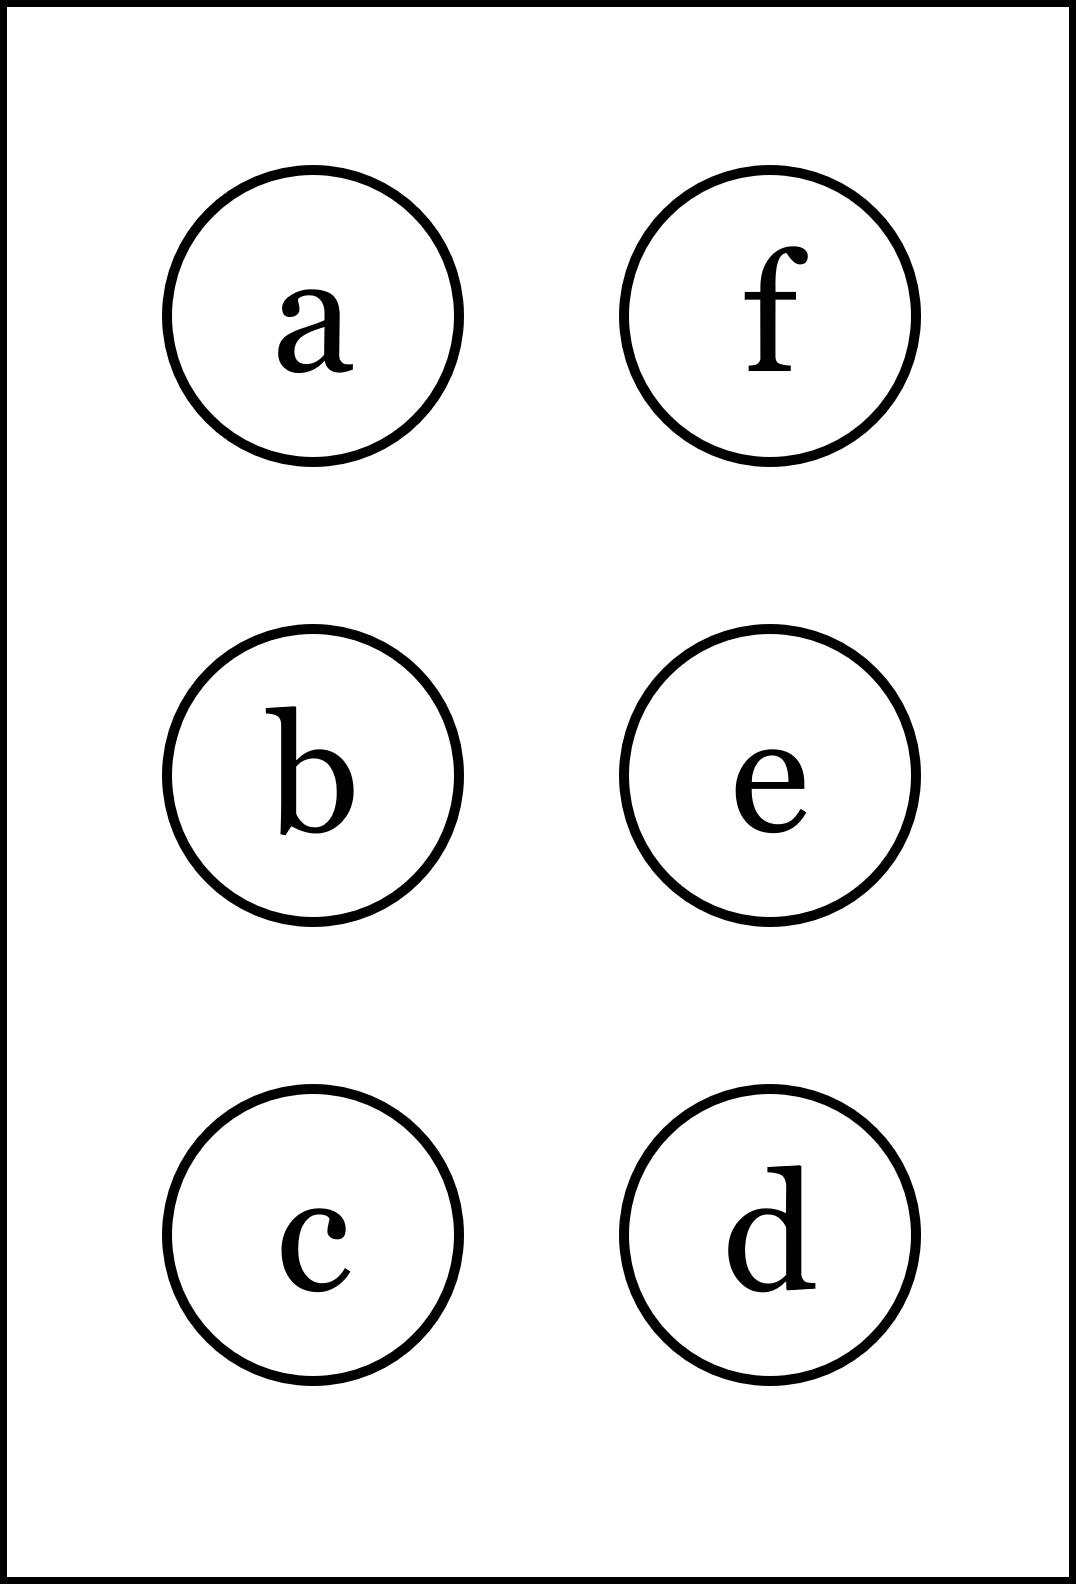
\includegraphics[height=40mm]{../images/braille.png}
{\small Písmeno Braillovej abecedy}
\end{center}
\end{minipage}
\end{center}
\end{minipage}
\\ \hdashline
\begin{minipage}[c][104.5mm][t]{0.5\linewidth}
\begin{center}
\vspace{7mm}
{\huge Závorky a zlomky, skupina \textit{Mu $\mu$} -\romannumeral3}\\[5mm]
\textit{Jméno:}\phantom{xxxxxxxxxxxxxxxxxxxxxxxxxxxxxxxxxxxxxxxxxxxxxxxxxxxxxxxxxxxxxxxxx}\\[5mm]
\begin{minipage}{0.95\linewidth}
\begin{center}
\textbf{Uprav výrazy (a) až (f)}. Pokud je výraz za otazníky roven výrazu pred otázniky, tak napravo obarvi príslušející kroužek. \textbf{Spolu odevzdejte výsledné slovo.}
\end{center}
\end{minipage}
\\[1mm]
\begin{minipage}{0.79\linewidth}
\begin{center}
\begin{varwidth}{\linewidth}
\begin{enumerate}
\normalsize
\item $2(8x+3)+5(-3-8x)$\quad \dotfill\; ???\;\dotfill \quad $-24x-9$
\item $-4(2+4x)(-6x-6)+3(-7+5x)$\quad \dotfill\; ???\;\dotfill \quad $96x^2+159x+27$
\item $(2x-4)^3-(4x+4)^2$\quad \dotfill\; ???\;\dotfill \quad $8x^3-64x^2+64x-80$
\item $\cfrac{9x+2}{3}+6\cfrac{2-3x}{-2}$\quad \dotfill\; ???\;\dotfill \quad $\cfrac{32}{6}$
\item $\cfrac{\frac{7}{2}-\frac{-9}{x}}{\frac{1}{-5}+\frac{3}{1}}$\quad \dotfill\; ???\;\dotfill \quad $\cfrac{-34x-91}{-28x}$
\item $\cfrac{(5-7x)^2-5}{(6x+2)\cdot\frac{2}{x}}$\quad \dotfill\; ???\;\dotfill \quad $\cfrac{49x^3-70x^2+20x}{12x+4}$
\end{enumerate}
\end{varwidth}
\end{center}
\end{minipage}
\begin{minipage}{0.20\linewidth}
\begin{center}
{\Huge\bfseries 3.} \\[2mm]
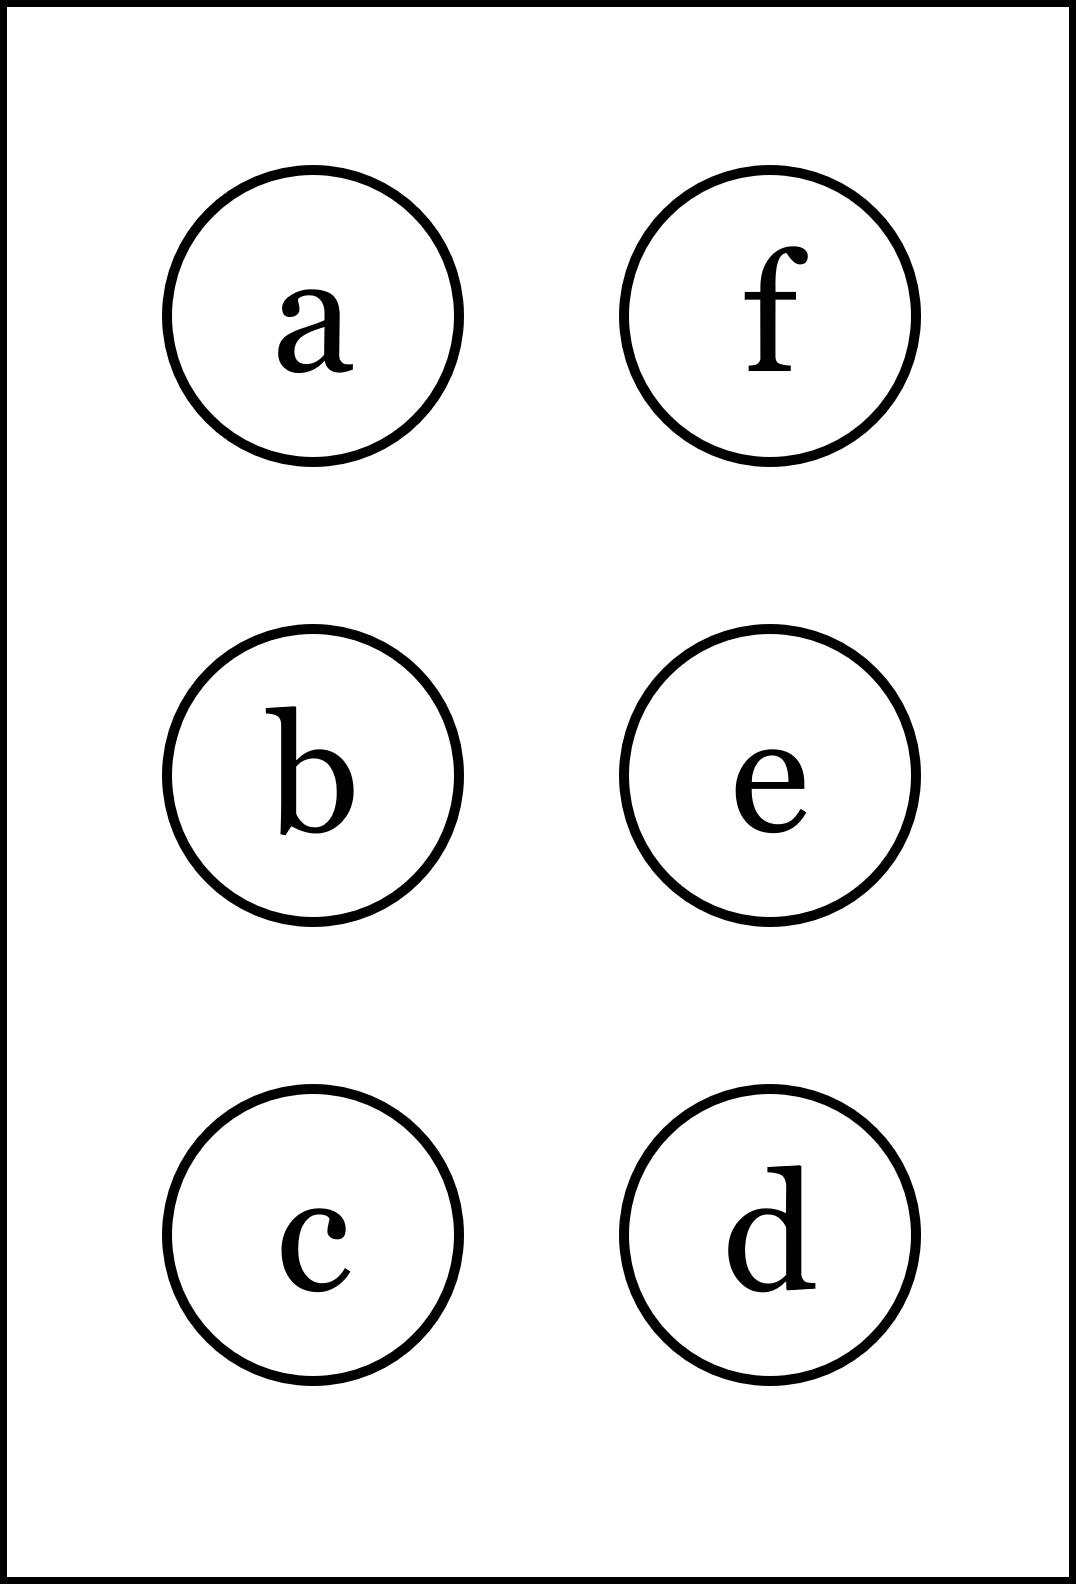
\includegraphics[height=40mm]{../images/braille.png}
{\small Písmeno Braillovej abecedy}
\end{center}
\end{minipage}
\end{center}
\end{minipage}
&
\begin{minipage}[c][104.5mm][t]{0.5\linewidth}
\begin{center}
\vspace{7mm}
{\huge Závorky a zlomky, skupina \textit{Mu $\mu$} -\romannumeral4}\\[5mm]
\textit{Jméno:}\phantom{xxxxxxxxxxxxxxxxxxxxxxxxxxxxxxxxxxxxxxxxxxxxxxxxxxxxxxxxxxxxxxxxx}\\[5mm]
\begin{minipage}{0.95\linewidth}
\begin{center}
\textbf{Uprav výrazy (a) až (f)}. Pokud je výraz za otazníky roven výrazu pred otázniky, tak napravo obarvi príslušející kroužek. \textbf{Spolu odevzdejte výsledné slovo.}
\end{center}
\end{minipage}
\\[1mm]
\begin{minipage}{0.79\linewidth}
\begin{center}
\begin{varwidth}{\linewidth}
\begin{enumerate}
\normalsize
\item $-8(-2x-6)+2(-9-8x)$\quad \dotfill\; ???\;\dotfill \quad $30$
\item $-2(-8+5x)(-x-2)+1(2+2x)$\quad \dotfill\; ???\;\dotfill \quad $10x^2-6x-30$
\item $(-x+2)^3-(4x+1)^2$\quad \dotfill\; ???\;\dotfill \quad $-x^3-10x^2-20x+7$
\item $\cfrac{5x+4}{-3}+4\cfrac{-1-4x}{2}$\quad \dotfill\; ???\;\dotfill \quad $\cfrac{58x+20}{-6}$
\item $\cfrac{\frac{-4}{4}-\frac{1}{x}}{\frac{1}{1}+\frac{-7}{2}}$\quad \dotfill\; ???\;\dotfill \quad $\cfrac{-8x-8}{-20x}$
\item $\cfrac{(5-3x)^2-5}{(2x-1)\cdot\frac{-6}{x}}$\quad \dotfill\; ???\;\dotfill \quad $\cfrac{9x^3-30x^2+20x}{-12x+6}$
\end{enumerate}
\end{varwidth}
\end{center}
\end{minipage}
\begin{minipage}{0.20\linewidth}
\begin{center}
{\Huge\bfseries 4.} \\[2mm]
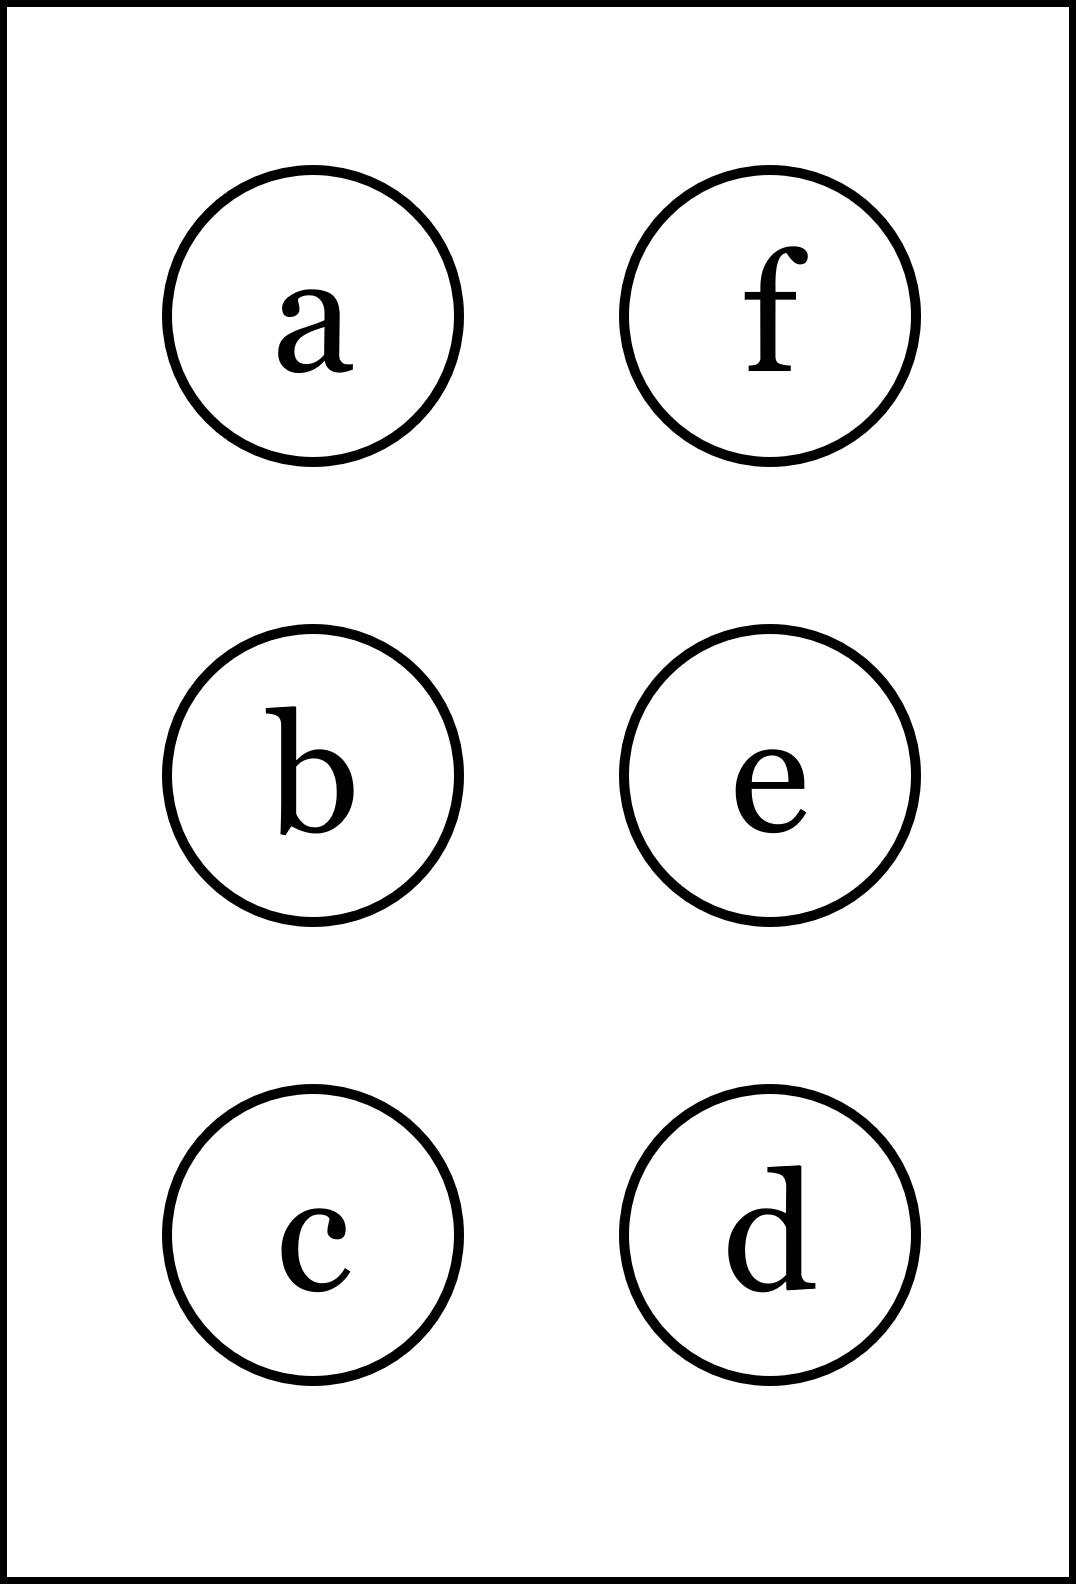
\includegraphics[height=40mm]{../images/braille.png}
{\small Písmeno Braillovej abecedy}
\end{center}
\end{minipage}
\end{center}
\end{minipage}
%
\end{tabular}
\newpage
\thispagestyle{empty}
\begin{tabular}{c:c}
\begin{minipage}[c][104.5mm][t]{0.5\linewidth}
\begin{center}
\vspace{7mm}
{\huge Závorky a zlomky, skupina \textit{Nu $\nu$} -\romannumeral1}\\[5mm]
\textit{Jméno:}\phantom{xxxxxxxxxxxxxxxxxxxxxxxxxxxxxxxxxxxxxxxxxxxxxxxxxxxxxxxxxxxxxxxxx}\\[5mm]
\begin{minipage}{0.95\linewidth}
\begin{center}
\textbf{Uprav výrazy (a) až (f)}. Pokud je výraz za otazníky roven výrazu pred otázniky, tak napravo obarvi príslušející kroužek. \textbf{Spolu odevzdejte výsledné slovo.}
\end{center}
\end{minipage}
\\[1mm]
\begin{minipage}{0.79\linewidth}
\begin{center}
\begin{varwidth}{\linewidth}
\begin{enumerate}
\normalsize
\item $-6(4x-3)+9(1-2x)$\quad \dotfill\; ???\;\dotfill \quad $-42x+27$
\item $-4(1+2x)(6x-1)+2(-3+3x)$\quad \dotfill\; ???\;\dotfill \quad $-48x^2+10x+2$
\item $(-x+1)^3-(7x+6)^2$\quad \dotfill\; ???\;\dotfill \quad $x^3-46x^2-87x-35$
\item $\cfrac{-3x-2}{-3}+3\cfrac{-4+8x}{3}$\quad \dotfill\; ???\;\dotfill \quad $\cfrac{-81x+30}{9}$
\item $\cfrac{\frac{3}{1}-\frac{4}{x}}{\frac{1}{8}+\frac{3}{3}}$\quad \dotfill\; ???\;\dotfill \quad $\cfrac{72x-96}{27x}$
\item $\cfrac{(-1+2x)^2+6}{(5x-4)\cdot\frac{2}{x}}$\quad \dotfill\; ???\;\dotfill \quad $\cfrac{4x^3-4x^2-7x}{-10x-8}$
\end{enumerate}
\end{varwidth}
\end{center}
\end{minipage}
\begin{minipage}{0.20\linewidth}
\begin{center}
{\Huge\bfseries 1.} \\[2mm]
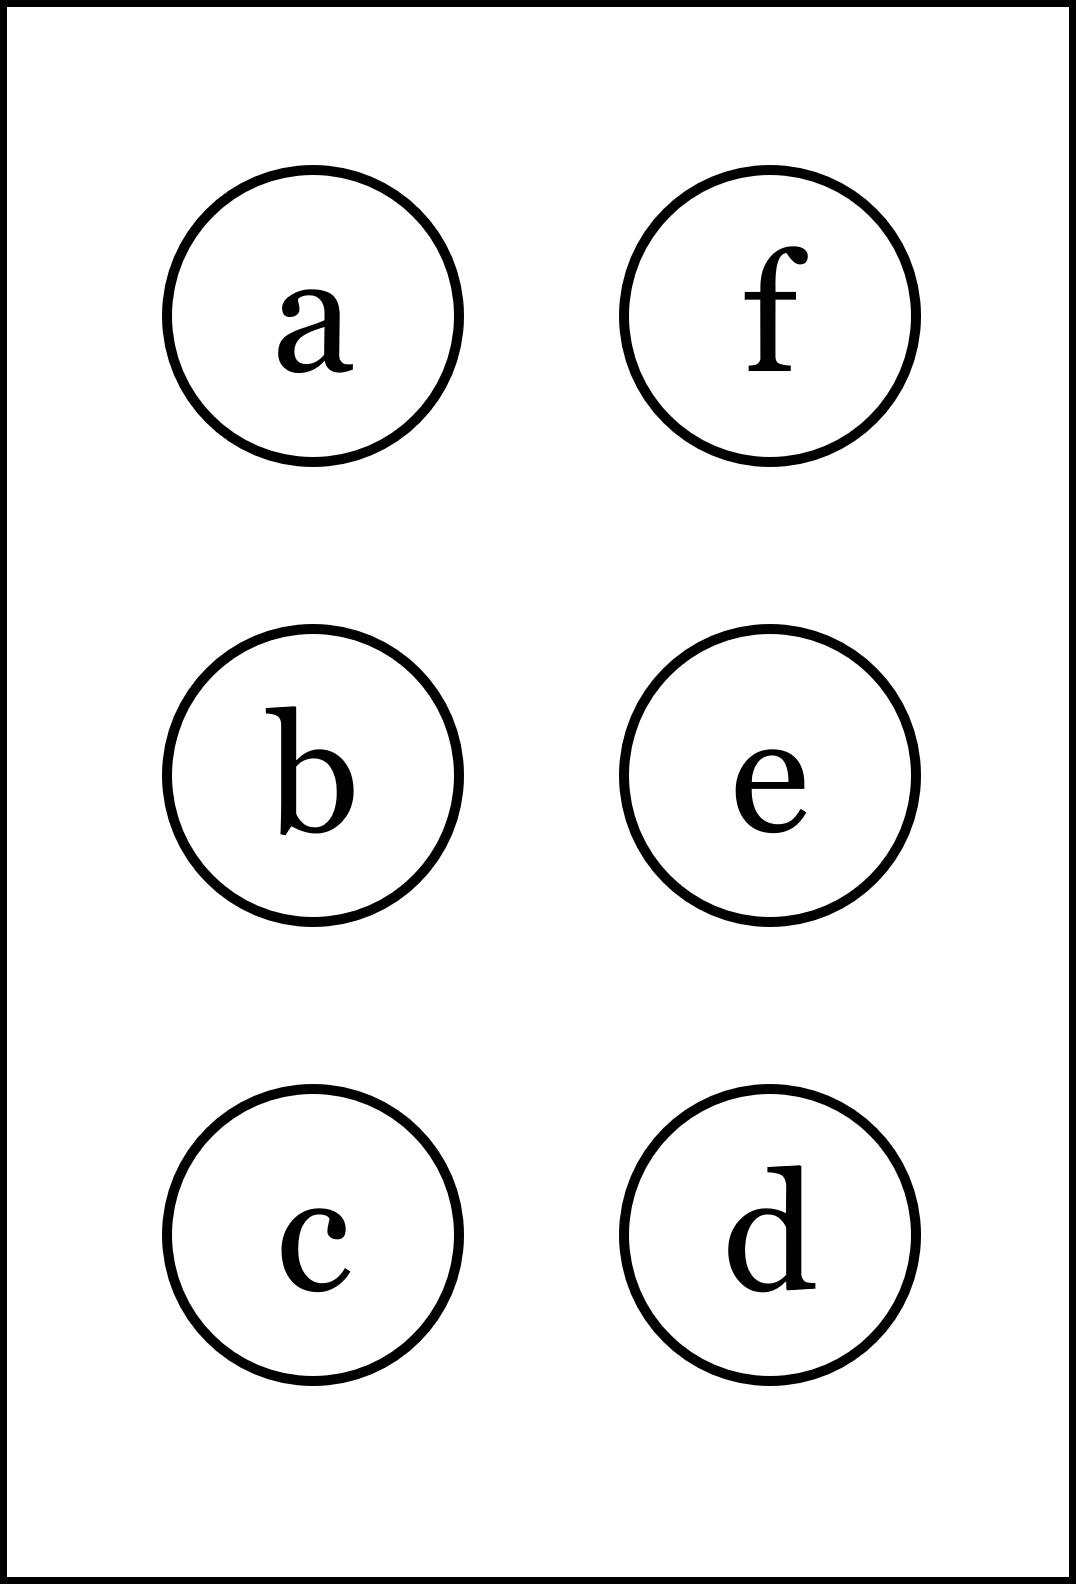
\includegraphics[height=40mm]{../images/braille.png}
{\small Písmeno Braillovej abecedy}
\end{center}
\end{minipage}
\end{center}
\end{minipage}
&
\begin{minipage}[c][104.5mm][t]{0.5\linewidth}
\begin{center}
\vspace{7mm}
{\huge Závorky a zlomky, skupina \textit{Nu $\nu$} -\romannumeral2}\\[5mm]
\textit{Jméno:}\phantom{xxxxxxxxxxxxxxxxxxxxxxxxxxxxxxxxxxxxxxxxxxxxxxxxxxxxxxxxxxxxxxxxx}\\[5mm]
\begin{minipage}{0.95\linewidth}
\begin{center}
\textbf{Uprav výrazy (a) až (f)}. Pokud je výraz za otazníky roven výrazu pred otázniky, tak napravo obarvi príslušející kroužek. \textbf{Spolu odevzdejte výsledné slovo.}
\end{center}
\end{minipage}
\\[1mm]
\begin{minipage}{0.79\linewidth}
\begin{center}
\begin{varwidth}{\linewidth}
\begin{enumerate}
\normalsize
\item $-9(-x-2)-1(-9-2x)$\quad \dotfill\; ???\;\dotfill \quad $11x+27$
\item $-3(1-x)(4x+2)-2(5+x)$\quad \dotfill\; ???\;\dotfill \quad $12x^2-8x-16$
\item $(-4x+1)^3-(7x-5)^2$\quad \dotfill\; ???\;\dotfill \quad $-64x^3-x^2+58x-24$
\item $\cfrac{2x+6}{-6}-4\cfrac{-2+x}{4}$\quad \dotfill\; ???\;\dotfill \quad $\cfrac{-32x-24}{24}$
\item $\cfrac{\frac{5}{-5}-\frac{-4}{x}}{\frac{1}{-2}+\frac{-8}{1}}$\quad \dotfill\; ???\;\dotfill \quad $\cfrac{-7x+41}{-85x}$
\item $\cfrac{(-1-3x)^2-6}{(-4x+8)\cdot\frac{1}{x}}$\quad \dotfill\; ???\;\dotfill \quad $\cfrac{9x^3+6x^2-5x}{-4x+8}$
\end{enumerate}
\end{varwidth}
\end{center}
\end{minipage}
\begin{minipage}{0.20\linewidth}
\begin{center}
{\Huge\bfseries 2.} \\[2mm]
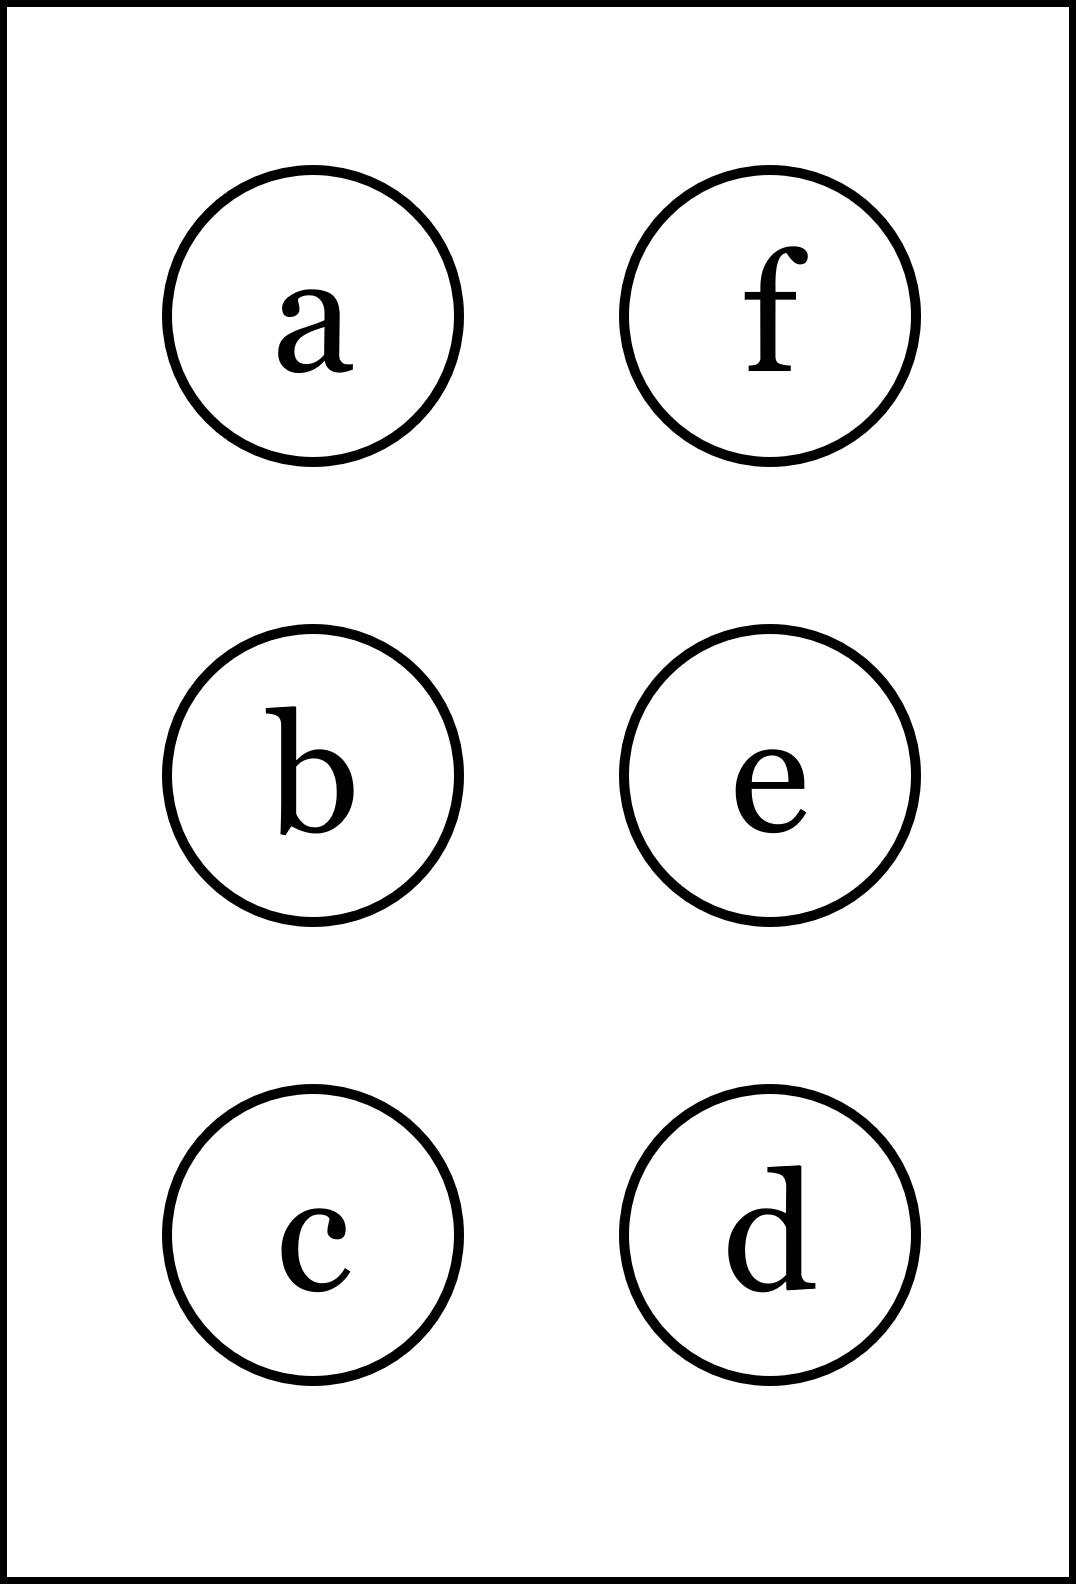
\includegraphics[height=40mm]{../images/braille.png}
{\small Písmeno Braillovej abecedy}
\end{center}
\end{minipage}
\end{center}
\end{minipage}
\\ \hdashline
\begin{minipage}[c][104.5mm][t]{0.5\linewidth}
\begin{center}
\vspace{7mm}
{\huge Závorky a zlomky, skupina \textit{Nu $\nu$} -\romannumeral3}\\[5mm]
\textit{Jméno:}\phantom{xxxxxxxxxxxxxxxxxxxxxxxxxxxxxxxxxxxxxxxxxxxxxxxxxxxxxxxxxxxxxxxxx}\\[5mm]
\begin{minipage}{0.95\linewidth}
\begin{center}
\textbf{Uprav výrazy (a) až (f)}. Pokud je výraz za otazníky roven výrazu pred otázniky, tak napravo obarvi príslušející kroužek. \textbf{Spolu odevzdejte výsledné slovo.}
\end{center}
\end{minipage}
\\[1mm]
\begin{minipage}{0.79\linewidth}
\begin{center}
\begin{varwidth}{\linewidth}
\begin{enumerate}
\normalsize
\item $-6(3x+2)-8(1-6x)$\quad \dotfill\; ???\;\dotfill \quad $30x-20$
\item $2(-2+x)(5x+7)-1(6+x)$\quad \dotfill\; ???\;\dotfill \quad $10x^2+7x+34$
\item $(-3x+1)^3-(-4x-4)^2$\quad \dotfill\; ???\;\dotfill \quad $-27x^3+11x^2-41x-15$
\item $\cfrac{x+2}{-6}-6\cfrac{2-x}{-9}$\quad \dotfill\; ???\;\dotfill \quad $\cfrac{45x+54}{-54}$
\item $\cfrac{\frac{8}{3}-\frac{-6}{x}}{\frac{1}{1}+\frac{-3}{-2}}$\quad \dotfill\; ???\;\dotfill \quad $\cfrac{-16x-36}{-15x}$
\item $\cfrac{(5-2x)^2-1}{(-2x+7)\cdot\frac{-6}{x}}$\quad \dotfill\; ???\;\dotfill \quad $\cfrac{4x^3-20x^2-24x}{-12x-42}$
\end{enumerate}
\end{varwidth}
\end{center}
\end{minipage}
\begin{minipage}{0.20\linewidth}
\begin{center}
{\Huge\bfseries 3.} \\[2mm]
\includegraphics[height=40mm]{../images/braille.png}
{\small Písmeno Braillovej abecedy}
\end{center}
\end{minipage}
\end{center}
\end{minipage}
&
\begin{minipage}[c][104.5mm][t]{0.5\linewidth}
\begin{center}
\vspace{7mm}
{\huge Závorky a zlomky, skupina \textit{Nu $\nu$} -\romannumeral4}\\[5mm]
\textit{Jméno:}\phantom{xxxxxxxxxxxxxxxxxxxxxxxxxxxxxxxxxxxxxxxxxxxxxxxxxxxxxxxxxxxxxxxxx}\\[5mm]
\begin{minipage}{0.95\linewidth}
\begin{center}
\textbf{Uprav výrazy (a) až (f)}. Pokud je výraz za otazníky roven výrazu pred otázniky, tak napravo obarvi príslušející kroužek. \textbf{Spolu odevzdejte výsledné slovo.}
\end{center}
\end{minipage}
\\[1mm]
\begin{minipage}{0.79\linewidth}
\begin{center}
\begin{varwidth}{\linewidth}
\begin{enumerate}
\normalsize
\item $7(4x+8)+6(-4-7x)$\quad \dotfill\; ???\;\dotfill \quad $-14x$
\item $-6(4-2x)(4x+1)+4(-1+2x)$\quad \dotfill\; ???\;\dotfill \quad $48x^2-76x-28$
\item $(4x-1)^3-(x+1)^2$\quad \dotfill\; ???\;\dotfill \quad $64x^3-49x^2+10x-2$
\item $\cfrac{5x+6}{5}+2\cfrac{-7+5x}{-3}$\quad \dotfill\; ???\;\dotfill \quad $\cfrac{35x-88}{15}$
\item $\cfrac{\frac{2}{-6}-\frac{-1}{x}}{\frac{1}{5}+\frac{-1}{-1}}$\quad \dotfill\; ???\;\dotfill \quad $\cfrac{-11x+32}{36x}$
\item $\cfrac{(5-2x)^2-1}{(4x-2)\cdot\frac{-4}{x}}$\quad \dotfill\; ???\;\dotfill \quad $\cfrac{4x^3-20x^2+24x}{-16x+8}$
\end{enumerate}
\end{varwidth}
\end{center}
\end{minipage}
\begin{minipage}{0.20\linewidth}
\begin{center}
{\Huge\bfseries 4.} \\[2mm]
\includegraphics[height=40mm]{../images/braille.png}
{\small Písmeno Braillovej abecedy}
\end{center}
\end{minipage}
\end{center}
\end{minipage}
%
\end{tabular}
\newpage
\thispagestyle{empty}
\begin{tabular}{c:c}
\begin{minipage}[c][104.5mm][t]{0.5\linewidth}
\begin{center}
\vspace{7mm}
{\huge Závorky a zlomky, skupina \textit{Xi $\xi$} -\romannumeral1}\\[5mm]
\textit{Jméno:}\phantom{xxxxxxxxxxxxxxxxxxxxxxxxxxxxxxxxxxxxxxxxxxxxxxxxxxxxxxxxxxxxxxxxx}\\[5mm]
\begin{minipage}{0.95\linewidth}
\begin{center}
\textbf{Uprav výrazy (a) až (f)}. Pokud je výraz za otazníky roven výrazu pred otázniky, tak napravo obarvi príslušející kroužek. \textbf{Spolu odevzdejte výsledné slovo.}
\end{center}
\end{minipage}
\\[1mm]
\begin{minipage}{0.79\linewidth}
\begin{center}
\begin{varwidth}{\linewidth}
\begin{enumerate}
\normalsize
\item $4(x+2)-3(-4-2x)$\quad \dotfill\; ???\;\dotfill \quad $10x+20$
\item $-2(-2+5x)(4x-2)+9(-6+5x)$\quad \dotfill\; ???\;\dotfill \quad $-40x^2+81x-62$
\item $(-x+2)^3-(8x-1)^2$\quad \dotfill\; ???\;\dotfill \quad $x^3-58x^2+4x+7$
\item $\cfrac{2x-2}{5}-2\cfrac{1+3x}{3}$\quad \dotfill\; ???\;\dotfill \quad $\cfrac{24x-16}{-15}$
\item $\cfrac{\frac{3}{4}-\frac{-1}{x}}{\frac{1}{3}+\frac{-2}{-1}}$\quad \dotfill\; ???\;\dotfill \quad $\cfrac{-7x-13}{-28x}$
\item $\cfrac{(-3+4x)^2-2}{(-4x+4)\cdot\frac{-5}{x}}$\quad \dotfill\; ???\;\dotfill \quad $\cfrac{16x^3-24x^2+7x}{20x-20}$
\end{enumerate}
\end{varwidth}
\end{center}
\end{minipage}
\begin{minipage}{0.20\linewidth}
\begin{center}
{\Huge\bfseries 1.} \\[2mm]
\includegraphics[height=40mm]{../images/braille.png}
{\small Písmeno Braillovej abecedy}
\end{center}
\end{minipage}
\end{center}
\end{minipage}
&
\begin{minipage}[c][104.5mm][t]{0.5\linewidth}
\begin{center}
\vspace{7mm}
{\huge Závorky a zlomky, skupina \textit{Xi $\xi$} -\romannumeral2}\\[5mm]
\textit{Jméno:}\phantom{xxxxxxxxxxxxxxxxxxxxxxxxxxxxxxxxxxxxxxxxxxxxxxxxxxxxxxxxxxxxxxxxx}\\[5mm]
\begin{minipage}{0.95\linewidth}
\begin{center}
\textbf{Uprav výrazy (a) až (f)}. Pokud je výraz za otazníky roven výrazu pred otázniky, tak napravo obarvi príslušející kroužek. \textbf{Spolu odevzdejte výsledné slovo.}
\end{center}
\end{minipage}
\\[1mm]
\begin{minipage}{0.79\linewidth}
\begin{center}
\begin{varwidth}{\linewidth}
\begin{enumerate}
\normalsize
\item $-7(3x+7)+2(4-8x)$\quad \dotfill\; ???\;\dotfill \quad $-37x-41$
\item $-3(-2+7x)(4x+1)+1(3-2x)$\quad \dotfill\; ???\;\dotfill \quad $-84x^2+x+9$
\item $(-x+1)^3-(-8x-1)^2$\quad \dotfill\; ???\;\dotfill \quad $-x^3-61x^2-19x$
\item $\cfrac{7x+1}{-3}-2\cfrac{-3+5x}{9}$\quad \dotfill\; ???\;\dotfill \quad $\cfrac{-93x-9}{27}$
\item $\cfrac{\frac{5}{-2}-\frac{-4}{x}}{\frac{1}{-3}+\frac{-1}{-2}}$\quad \dotfill\; ???\;\dotfill \quad $\cfrac{33x-51}{-2x}$
\item $\cfrac{(-4-2x)^2-1}{(-x-5)\cdot\frac{-4}{x}}$\quad \dotfill\; ???\;\dotfill \quad $\cfrac{4x^3+16x^2-15x}{-4x+20}$
\end{enumerate}
\end{varwidth}
\end{center}
\end{minipage}
\begin{minipage}{0.20\linewidth}
\begin{center}
{\Huge\bfseries 2.} \\[2mm]
\includegraphics[height=40mm]{../images/braille.png}
{\small Písmeno Braillovej abecedy}
\end{center}
\end{minipage}
\end{center}
\end{minipage}
\\ \hdashline
\begin{minipage}[c][104.5mm][t]{0.5\linewidth}
\begin{center}
\vspace{7mm}
{\huge Závorky a zlomky, skupina \textit{Xi $\xi$} -\romannumeral3}\\[5mm]
\textit{Jméno:}\phantom{xxxxxxxxxxxxxxxxxxxxxxxxxxxxxxxxxxxxxxxxxxxxxxxxxxxxxxxxxxxxxxxxx}\\[5mm]
\begin{minipage}{0.95\linewidth}
\begin{center}
\textbf{Uprav výrazy (a) až (f)}. Pokud je výraz za otazníky roven výrazu pred otázniky, tak napravo obarvi príslušející kroužek. \textbf{Spolu odevzdejte výsledné slovo.}
\end{center}
\end{minipage}
\\[1mm]
\begin{minipage}{0.79\linewidth}
\begin{center}
\begin{varwidth}{\linewidth}
\begin{enumerate}
\normalsize
\item $2(4x-1)+6(-5-6x)$\quad \dotfill\; ???\;\dotfill \quad $-28x-32$
\item $2(1+4x)(7x-3)+9(7-x)$\quad \dotfill\; ???\;\dotfill \quad $56x^2+19x$
\item $(3x+3)^3-(-x+4)^2$\quad \dotfill\; ???\;\dotfill \quad $-27x^3-80x^2+11$
\item $\cfrac{3x-2}{2}-3\cfrac{-1-x}{3}$\quad \dotfill\; ???\;\dotfill \quad $\cfrac{0}{-6}$
\item $\cfrac{\frac{-2}{-7}-\frac{5}{x}}{\frac{1}{1}+\frac{2}{2}}$\quad \dotfill\; ???\;\dotfill \quad $\cfrac{-4x+70}{-28x}$
\item $\cfrac{(4+6x)^2-4}{(-4x-6)\cdot\frac{6}{x}}$\quad \dotfill\; ???\;\dotfill \quad $\cfrac{36x^3+48x^2-12x}{24x-36}$
\end{enumerate}
\end{varwidth}
\end{center}
\end{minipage}
\begin{minipage}{0.20\linewidth}
\begin{center}
{\Huge\bfseries 3.} \\[2mm]
\includegraphics[height=40mm]{../images/braille.png}
{\small Písmeno Braillovej abecedy}
\end{center}
\end{minipage}
\end{center}
\end{minipage}
&
\begin{minipage}[c][104.5mm][t]{0.5\linewidth}
\begin{center}
\vspace{7mm}
{\huge Závorky a zlomky, skupina \textit{Xi $\xi$} -\romannumeral4}\\[5mm]
\textit{Jméno:}\phantom{xxxxxxxxxxxxxxxxxxxxxxxxxxxxxxxxxxxxxxxxxxxxxxxxxxxxxxxxxxxxxxxxx}\\[5mm]
\begin{minipage}{0.95\linewidth}
\begin{center}
\textbf{Uprav výrazy (a) až (f)}. Pokud je výraz za otazníky roven výrazu pred otázniky, tak napravo obarvi príslušející kroužek. \textbf{Spolu odevzdejte výsledné slovo.}
\end{center}
\end{minipage}
\\[1mm]
\begin{minipage}{0.79\linewidth}
\begin{center}
\begin{varwidth}{\linewidth}
\begin{enumerate}
\normalsize
\item $-9(-4x+6)-6(3-5x)$\quad \dotfill\; ???\;\dotfill \quad $66x-72$
\item $4(3-x)(-x-5)-5(2+2x)$\quad \dotfill\; ???\;\dotfill \quad $4x^2+2x-70$
\item $(-4x+2)^3-(-x+2)^2$\quad \dotfill\; ???\;\dotfill \quad $-64x^3+95x^2-44x+4$
\item $\cfrac{-2x+4}{-9}-3\cfrac{-1+2x}{-3}$\quad \dotfill\; ???\;\dotfill \quad $\cfrac{-60x-39}{-27}$
\item $\cfrac{\frac{-7}{2}-\frac{-6}{x}}{\frac{1}{5}+\frac{-2}{1}}$\quad \dotfill\; ???\;\dotfill \quad $\cfrac{-32x+57}{-18x}$
\item $\cfrac{(-1+5x)^2+1}{(6x+3)\cdot\frac{4}{x}}$\quad \dotfill\; ???\;\dotfill \quad $\cfrac{25x^3-10x^2-2x}{-24x+12}$
\end{enumerate}
\end{varwidth}
\end{center}
\end{minipage}
\begin{minipage}{0.20\linewidth}
\begin{center}
{\Huge\bfseries 4.} \\[2mm]
\includegraphics[height=40mm]{../images/braille.png}
{\small Písmeno Braillovej abecedy}
\end{center}
\end{minipage}
\end{center}
\end{minipage}
%
\end{tabular}
\newpage
\thispagestyle{empty}
\begin{tabular}{c:c}
\begin{minipage}[c][104.5mm][t]{0.5\linewidth}
\begin{center}
\vspace{7mm}
{\huge Závorky a zlomky, skupina \textit{Omicron $\omicron$} -\romannumeral1}\\[5mm]
\textit{Jméno:}\phantom{xxxxxxxxxxxxxxxxxxxxxxxxxxxxxxxxxxxxxxxxxxxxxxxxxxxxxxxxxxxxxxxxx}\\[5mm]
\begin{minipage}{0.95\linewidth}
\begin{center}
\textbf{Uprav výrazy (a) až (f)}. Pokud je výraz za otazníky roven výrazu pred otázniky, tak napravo obarvi príslušející kroužek. \textbf{Spolu odevzdejte výsledné slovo.}
\end{center}
\end{minipage}
\\[1mm]
\begin{minipage}{0.79\linewidth}
\begin{center}
\begin{varwidth}{\linewidth}
\begin{enumerate}
\normalsize
\item $-9(x+3)-4(8-2x)$\quad \dotfill\; ???\;\dotfill \quad $-x-59$
\item $-2(2-x)(x+1)-7(-3-x)$\quad \dotfill\; ???\;\dotfill \quad $2x^2-5x-17$
\item $(-2x+3)^3-(-5x-4)^2$\quad \dotfill\; ???\;\dotfill \quad $-8x^3+11x^2-94x+11$
\item $\cfrac{x-6}{6}-2\cfrac{-3-4x}{-3}$\quad \dotfill\; ???\;\dotfill \quad $\cfrac{45x+54}{18}$
\item $\cfrac{\frac{1}{-6}-\frac{-3}{x}}{\frac{1}{1}+\frac{-1}{-2}}$\quad \dotfill\; ???\;\dotfill \quad $\cfrac{-2x+36}{18x}$
\item $\cfrac{(7+6x)^2-1}{(-6x-7)\cdot\frac{3}{x}}$\quad \dotfill\; ???\;\dotfill \quad $\cfrac{36x^3+84x^2-48x}{18x-21}$
\end{enumerate}
\end{varwidth}
\end{center}
\end{minipage}
\begin{minipage}{0.20\linewidth}
\begin{center}
{\Huge\bfseries 1.} \\[2mm]
\includegraphics[height=40mm]{../images/braille.png}
{\small Písmeno Braillovej abecedy}
\end{center}
\end{minipage}
\end{center}
\end{minipage}
&
\begin{minipage}[c][104.5mm][t]{0.5\linewidth}
\begin{center}
\vspace{7mm}
{\huge Závorky a zlomky, skupina \textit{Omicron $\omicron$} -\romannumeral2}\\[5mm]
\textit{Jméno:}\phantom{xxxxxxxxxxxxxxxxxxxxxxxxxxxxxxxxxxxxxxxxxxxxxxxxxxxxxxxxxxxxxxxxx}\\[5mm]
\begin{minipage}{0.95\linewidth}
\begin{center}
\textbf{Uprav výrazy (a) až (f)}. Pokud je výraz za otazníky roven výrazu pred otázniky, tak napravo obarvi príslušející kroužek. \textbf{Spolu odevzdejte výsledné slovo.}
\end{center}
\end{minipage}
\\[1mm]
\begin{minipage}{0.79\linewidth}
\begin{center}
\begin{varwidth}{\linewidth}
\begin{enumerate}
\normalsize
\item $3(-2x-3)+6(2+x)$\quad \dotfill\; ???\;\dotfill \quad $3$
\item $7(3-2x)(2x+2)-4(-5+6x)$\quad \dotfill\; ???\;\dotfill \quad $-28x^2+10x-62$
\item $(-x+2)^3-(-5x-9)^2$\quad \dotfill\; ???\;\dotfill \quad $-x^3-19x^2-102x-73$
\item $\cfrac{-5x-2}{4}+2\cfrac{-1-x}{3}$\quad \dotfill\; ???\;\dotfill \quad $\cfrac{23x-14}{-12}$
\item $\cfrac{\frac{3}{5}-\frac{-2}{x}}{\frac{1}{-1}+\frac{-1}{3}}$\quad \dotfill\; ???\;\dotfill \quad $\cfrac{-10x-33}{20x}$
\item $\cfrac{(-3+3x)^2+9}{(5x-1)\cdot\frac{-4}{x}}$\quad \dotfill\; ???\;\dotfill \quad $\cfrac{9x^3-18x^2-18x}{20x+4}$
\end{enumerate}
\end{varwidth}
\end{center}
\end{minipage}
\begin{minipage}{0.20\linewidth}
\begin{center}
{\Huge\bfseries 2.} \\[2mm]
\includegraphics[height=40mm]{../images/braille.png}
{\small Písmeno Braillovej abecedy}
\end{center}
\end{minipage}
\end{center}
\end{minipage}
\\ \hdashline
\begin{minipage}[c][104.5mm][t]{0.5\linewidth}
\begin{center}
\vspace{7mm}
{\huge Závorky a zlomky, skupina \textit{Omicron $\omicron$} -\romannumeral3}\\[5mm]
\textit{Jméno:}\phantom{xxxxxxxxxxxxxxxxxxxxxxxxxxxxxxxxxxxxxxxxxxxxxxxxxxxxxxxxxxxxxxxxx}\\[5mm]
\begin{minipage}{0.95\linewidth}
\begin{center}
\textbf{Uprav výrazy (a) až (f)}. Pokud je výraz za otazníky roven výrazu pred otázniky, tak napravo obarvi príslušející kroužek. \textbf{Spolu odevzdejte výsledné slovo.}
\end{center}
\end{minipage}
\\[1mm]
\begin{minipage}{0.79\linewidth}
\begin{center}
\begin{varwidth}{\linewidth}
\begin{enumerate}
\normalsize
\item $-3(-6x-3)+2(-2+3x)$\quad \dotfill\; ???\;\dotfill \quad $24x+5$
\item $-4(-5+7x)(-x+2)+5(6-5x)$\quad \dotfill\; ???\;\dotfill \quad $28x^2+101x-70$
\item $(4x+3)^3-(-5x-8)^2$\quad \dotfill\; ???\;\dotfill \quad $64x^3+119x^2+28x-37$
\item $\cfrac{5x+7}{-2}-2\cfrac{-9-4x}{-3}$\quad \dotfill\; ???\;\dotfill \quad $\cfrac{-31x-57}{-6}$
\item $\cfrac{\frac{7}{-4}-\frac{1}{x}}{\frac{1}{3}+\frac{-3}{1}}$\quad \dotfill\; ???\;\dotfill \quad $\cfrac{21x+12}{32x}$
\item $\cfrac{(-4+3x)^2+2}{(2x-1)\cdot\frac{-2}{x}}$\quad \dotfill\; ???\;\dotfill \quad $\cfrac{9x^3-24x^2+18x}{-4x+2}$
\end{enumerate}
\end{varwidth}
\end{center}
\end{minipage}
\begin{minipage}{0.20\linewidth}
\begin{center}
{\Huge\bfseries 3.} \\[2mm]
\includegraphics[height=40mm]{../images/braille.png}
{\small Písmeno Braillovej abecedy}
\end{center}
\end{minipage}
\end{center}
\end{minipage}
&
\begin{minipage}[c][104.5mm][t]{0.5\linewidth}
\begin{center}
\vspace{7mm}
{\huge Závorky a zlomky, skupina \textit{Omicron $\omicron$} -\romannumeral4}\\[5mm]
\textit{Jméno:}\phantom{xxxxxxxxxxxxxxxxxxxxxxxxxxxxxxxxxxxxxxxxxxxxxxxxxxxxxxxxxxxxxxxxx}\\[5mm]
\begin{minipage}{0.95\linewidth}
\begin{center}
\textbf{Uprav výrazy (a) až (f)}. Pokud je výraz za otazníky roven výrazu pred otázniky, tak napravo obarvi príslušející kroužek. \textbf{Spolu odevzdejte výsledné slovo.}
\end{center}
\end{minipage}
\\[1mm]
\begin{minipage}{0.79\linewidth}
\begin{center}
\begin{varwidth}{\linewidth}
\begin{enumerate}
\normalsize
\item $-2(-3x+8)+5(6-2x)$\quad \dotfill\; ???\;\dotfill \quad $-4x+14$
\item $-6(1+x)(9x+4)-6(5-2x)$\quad \dotfill\; ???\;\dotfill \quad $-54x^2+66x+54$
\item $(-4x+2)^3-(2x+2)^2$\quad \dotfill\; ???\;\dotfill \quad $-64x^3+92x^2-56x+4$
\item $\cfrac{2x-1}{-2}+7\cfrac{-4+5x}{-8}$\quad \dotfill\; ???\;\dotfill \quad $\cfrac{64}{-16}$
\item $\cfrac{\frac{2}{-5}-\frac{-1}{x}}{\frac{1}{3}+\frac{-6}{4}}$\quad \dotfill\; ???\;\dotfill \quad $\cfrac{24x-60}{70x}$
\item $\cfrac{(-1-2x)^2-2}{(-2x+2)\cdot\frac{-2}{x}}$\quad \dotfill\; ???\;\dotfill \quad $\cfrac{4x^3+4x^2+x}{-4x-4}$
\end{enumerate}
\end{varwidth}
\end{center}
\end{minipage}
\begin{minipage}{0.20\linewidth}
\begin{center}
{\Huge\bfseries 4.} \\[2mm]
\includegraphics[height=40mm]{../images/braille.png}
{\small Písmeno Braillovej abecedy}
\end{center}
\end{minipage}
\end{center}
\end{minipage}
%
\end{tabular}
\newpage
\thispagestyle{empty}
\begin{tabular}{c:c}
\begin{minipage}[c][104.5mm][t]{0.5\linewidth}
\begin{center}
\vspace{7mm}
{\huge Závorky a zlomky, skupina \textit{Pi $\pi$} -\romannumeral1}\\[5mm]
\textit{Jméno:}\phantom{xxxxxxxxxxxxxxxxxxxxxxxxxxxxxxxxxxxxxxxxxxxxxxxxxxxxxxxxxxxxxxxxx}\\[5mm]
\begin{minipage}{0.95\linewidth}
\begin{center}
\textbf{Uprav výrazy (a) až (f)}. Pokud je výraz za otazníky roven výrazu pred otázniky, tak napravo obarvi príslušející kroužek. \textbf{Spolu odevzdejte výsledné slovo.}
\end{center}
\end{minipage}
\\[1mm]
\begin{minipage}{0.79\linewidth}
\begin{center}
\begin{varwidth}{\linewidth}
\begin{enumerate}
\normalsize
\item $-3(2x-6)-3(7+4x)$\quad \dotfill\; ???\;\dotfill \quad $-18x-3$
\item $2(5+x)(-6x-2)+2(-8+6x)$\quad \dotfill\; ???\;\dotfill \quad $-12x^2+52x+36$
\item $(-2x+4)^3-(4x-6)^2$\quad \dotfill\; ???\;\dotfill \quad $8x^3+32x^2-48x+28$
\item $\cfrac{-5x-3}{3}-6\cfrac{-3-2x}{3}$\quad \dotfill\; ???\;\dotfill \quad $\cfrac{21x+45}{-9}$
\item $\cfrac{\frac{-2}{3}-\frac{1}{x}}{\frac{1}{1}+\frac{-2}{-2}}$\quad \dotfill\; ???\;\dotfill \quad $\cfrac{4x+6}{-12x}$
\item $\cfrac{(1-6x)^2-3}{(2x+7)\cdot\frac{-8}{x}}$\quad \dotfill\; ???\;\dotfill \quad $\cfrac{36x^3-12x^2+2x}{16x-56}$
\end{enumerate}
\end{varwidth}
\end{center}
\end{minipage}
\begin{minipage}{0.20\linewidth}
\begin{center}
{\Huge\bfseries 1.} \\[2mm]
\includegraphics[height=40mm]{../images/braille.png}
{\small Písmeno Braillovej abecedy}
\end{center}
\end{minipage}
\end{center}
\end{minipage}
&
\begin{minipage}[c][104.5mm][t]{0.5\linewidth}
\begin{center}
\vspace{7mm}
{\huge Závorky a zlomky, skupina \textit{Pi $\pi$} -\romannumeral2}\\[5mm]
\textit{Jméno:}\phantom{xxxxxxxxxxxxxxxxxxxxxxxxxxxxxxxxxxxxxxxxxxxxxxxxxxxxxxxxxxxxxxxxx}\\[5mm]
\begin{minipage}{0.95\linewidth}
\begin{center}
\textbf{Uprav výrazy (a) až (f)}. Pokud je výraz za otazníky roven výrazu pred otázniky, tak napravo obarvi príslušející kroužek. \textbf{Spolu odevzdejte výsledné slovo.}
\end{center}
\end{minipage}
\\[1mm]
\begin{minipage}{0.79\linewidth}
\begin{center}
\begin{varwidth}{\linewidth}
\begin{enumerate}
\normalsize
\item $-5(6x-7)-7(3-2x)$\quad \dotfill\; ???\;\dotfill \quad $-16x+14$
\item $6(-1-6x)(-2x+1)+4(5+4x)$\quad \dotfill\; ???\;\dotfill \quad $72x^2+8x+14$
\item $(-x+2)^3-(x-3)^2$\quad \dotfill\; ???\;\dotfill \quad $-x^3+5x^2-6x-1$
\item $\cfrac{-2x+5}{2}+4\cfrac{9+3x}{2}$\quad \dotfill\; ???\;\dotfill \quad $\cfrac{20x+82}{-4}$
\item $\cfrac{\frac{-7}{-3}-\frac{-4}{x}}{\frac{1}{-2}+\frac{1}{-1}}$\quad \dotfill\; ???\;\dotfill \quad $\cfrac{-12x-23}{9x}$
\item $\cfrac{(-4-4x)^2-6}{(8x+5)\cdot\frac{2}{x}}$\quad \dotfill\; ???\;\dotfill \quad $\cfrac{16x^3+32x^2+10x}{16x+10}$
\end{enumerate}
\end{varwidth}
\end{center}
\end{minipage}
\begin{minipage}{0.20\linewidth}
\begin{center}
{\Huge\bfseries 2.} \\[2mm]
\includegraphics[height=40mm]{../images/braille.png}
{\small Písmeno Braillovej abecedy}
\end{center}
\end{minipage}
\end{center}
\end{minipage}
\\ \hdashline
\begin{minipage}[c][104.5mm][t]{0.5\linewidth}
\begin{center}
\vspace{7mm}
{\huge Závorky a zlomky, skupina \textit{Pi $\pi$} -\romannumeral3}\\[5mm]
\textit{Jméno:}\phantom{xxxxxxxxxxxxxxxxxxxxxxxxxxxxxxxxxxxxxxxxxxxxxxxxxxxxxxxxxxxxxxxxx}\\[5mm]
\begin{minipage}{0.95\linewidth}
\begin{center}
\textbf{Uprav výrazy (a) až (f)}. Pokud je výraz za otazníky roven výrazu pred otázniky, tak napravo obarvi príslušející kroužek. \textbf{Spolu odevzdejte výsledné slovo.}
\end{center}
\end{minipage}
\\[1mm]
\begin{minipage}{0.79\linewidth}
\begin{center}
\begin{varwidth}{\linewidth}
\begin{enumerate}
\normalsize
\item $8(5x+3)-2(4+6x)$\quad \dotfill\; ???\;\dotfill \quad $28x$
\item $-4(-5-x)(2x-4)-5(-5-2x)$\quad \dotfill\; ???\;\dotfill \quad $8x^2+34x-55$
\item $(2x-2)^3-(-5x+7)^2$\quad \dotfill\; ???\;\dotfill \quad $-8x^3+49x^2+94x-57$
\item $\cfrac{8x-5}{2}-8\cfrac{1+5x}{9}$\quad \dotfill\; ???\;\dotfill \quad $\cfrac{8x-61}{-18}$
\item $\cfrac{\frac{6}{5}-\frac{1}{x}}{\frac{1}{1}+\frac{-2}{-8}}$\quad \dotfill\; ???\;\dotfill \quad $\cfrac{-47x+37}{-50x}$
\item $\cfrac{(-2-4x)^2+6}{(-6x-3)\cdot\frac{-7}{x}}$\quad \dotfill\; ???\;\dotfill \quad $\cfrac{16x^3+16x^2+10x}{42x+21}$
\end{enumerate}
\end{varwidth}
\end{center}
\end{minipage}
\begin{minipage}{0.20\linewidth}
\begin{center}
{\Huge\bfseries 3.} \\[2mm]
\includegraphics[height=40mm]{../images/braille.png}
{\small Písmeno Braillovej abecedy}
\end{center}
\end{minipage}
\end{center}
\end{minipage}
&
\begin{minipage}[c][104.5mm][t]{0.5\linewidth}
\begin{center}
\vspace{7mm}
{\huge Závorky a zlomky, skupina \textit{Pi $\pi$} -\romannumeral4}\\[5mm]
\textit{Jméno:}\phantom{xxxxxxxxxxxxxxxxxxxxxxxxxxxxxxxxxxxxxxxxxxxxxxxxxxxxxxxxxxxxxxxxx}\\[5mm]
\begin{minipage}{0.95\linewidth}
\begin{center}
\textbf{Uprav výrazy (a) až (f)}. Pokud je výraz za otazníky roven výrazu pred otázniky, tak napravo obarvi príslušející kroužek. \textbf{Spolu odevzdejte výsledné slovo.}
\end{center}
\end{minipage}
\\[1mm]
\begin{minipage}{0.79\linewidth}
\begin{center}
\begin{varwidth}{\linewidth}
\begin{enumerate}
\normalsize
\item $6(-x+1)+1(-5+6x)$\quad \dotfill\; ???\;\dotfill \quad $1$
\item $-2(-6+2x)(x-7)+8(-7+x)$\quad \dotfill\; ???\;\dotfill \quad $-4x^2+48x-140$
\item $(x+2)^3-(9x-6)^2$\quad \dotfill\; ???\;\dotfill \quad $x^3-75x^2+120x-28$
\item $\cfrac{-x+1}{-2}-6\cfrac{-1+4x}{6}$\quad \dotfill\; ???\;\dotfill \quad $\cfrac{-6}{12}$
\item $\cfrac{\frac{-2}{8}-\frac{4}{x}}{\frac{1}{1}+\frac{-1}{-2}}$\quad \dotfill\; ???\;\dotfill \quad $\cfrac{5x+61}{-24x}$
\item $\cfrac{(4-x)^2+2}{(x-4)\cdot\frac{3}{x}}$\quad \dotfill\; ???\;\dotfill \quad $\cfrac{x^3-8x^2-18x}{-3x-12}$
\end{enumerate}
\end{varwidth}
\end{center}
\end{minipage}
\begin{minipage}{0.20\linewidth}
\begin{center}
{\Huge\bfseries 4.} \\[2mm]
\includegraphics[height=40mm]{../images/braille.png}
{\small Písmeno Braillovej abecedy}
\end{center}
\end{minipage}
\end{center}
\end{minipage}
%
\end{tabular}
\newpage
\thispagestyle{empty}
\begin{tabular}{c:c}
\begin{minipage}[c][104.5mm][t]{0.5\linewidth}
\begin{center}
\vspace{7mm}
{\huge Závorky a zlomky, skupina \textit{Rho $\rho$} -\romannumeral1}\\[5mm]
\textit{Jméno:}\phantom{xxxxxxxxxxxxxxxxxxxxxxxxxxxxxxxxxxxxxxxxxxxxxxxxxxxxxxxxxxxxxxxxx}\\[5mm]
\begin{minipage}{0.95\linewidth}
\begin{center}
\textbf{Uprav výrazy (a) až (f)}. Pokud je výraz za otazníky roven výrazu pred otázniky, tak napravo obarvi príslušející kroužek. \textbf{Spolu odevzdejte výsledné slovo.}
\end{center}
\end{minipage}
\\[1mm]
\begin{minipage}{0.79\linewidth}
\begin{center}
\begin{varwidth}{\linewidth}
\begin{enumerate}
\normalsize
\item $3(-6x-9)+6(-2-7x)$\quad \dotfill\; ???\;\dotfill \quad $-60x+39$
\item $2(-5-9x)(-4x-3)+1(3+3x)$\quad \dotfill\; ???\;\dotfill \quad $72x^2+97x+33$
\item $(-x+1)^3-(9x+2)^2$\quad \dotfill\; ???\;\dotfill \quad $x^3+78x^2-39x-3$
\item $\cfrac{-2x+2}{4}+4\cfrac{-4-4x}{5}$\quad \dotfill\; ???\;\dotfill \quad $\cfrac{-54}{-20}$
\item $\cfrac{\frac{1}{2}-\frac{2}{x}}{\frac{1}{3}+\frac{1}{1}}$\quad \dotfill\; ???\;\dotfill \quad $\cfrac{4x-11}{8x}$
\item $\cfrac{(-3+4x)^2-6}{(4x-6)\cdot\frac{-1}{x}}$\quad \dotfill\; ???\;\dotfill \quad $\cfrac{16x^3-24x^2+3x}{-4x+6}$
\end{enumerate}
\end{varwidth}
\end{center}
\end{minipage}
\begin{minipage}{0.20\linewidth}
\begin{center}
{\Huge\bfseries 1.} \\[2mm]
\includegraphics[height=40mm]{../images/braille.png}
{\small Písmeno Braillovej abecedy}
\end{center}
\end{minipage}
\end{center}
\end{minipage}
&
\begin{minipage}[c][104.5mm][t]{0.5\linewidth}
\begin{center}
\vspace{7mm}
{\huge Závorky a zlomky, skupina \textit{Rho $\rho$} -\romannumeral2}\\[5mm]
\textit{Jméno:}\phantom{xxxxxxxxxxxxxxxxxxxxxxxxxxxxxxxxxxxxxxxxxxxxxxxxxxxxxxxxxxxxxxxxx}\\[5mm]
\begin{minipage}{0.95\linewidth}
\begin{center}
\textbf{Uprav výrazy (a) až (f)}. Pokud je výraz za otazníky roven výrazu pred otázniky, tak napravo obarvi príslušející kroužek. \textbf{Spolu odevzdejte výsledné slovo.}
\end{center}
\end{minipage}
\\[1mm]
\begin{minipage}{0.79\linewidth}
\begin{center}
\begin{varwidth}{\linewidth}
\begin{enumerate}
\normalsize
\item $2(-7x+2)+8(3-7x)$\quad \dotfill\; ???\;\dotfill \quad $-70x+28$
\item $2(-3-5x)(6x+9)-3(1+x)$\quad \dotfill\; ???\;\dotfill \quad $-60x^2-129x-57$
\item $(2x+4)^3-(x-5)^2$\quad \dotfill\; ???\;\dotfill \quad $-8x^3+47x^2+106x+39$
\item $\cfrac{-7x-1}{8}-3\cfrac{4+2x}{5}$\quad \dotfill\; ???\;\dotfill \quad $\cfrac{-101}{-40}$
\item $\cfrac{\frac{2}{3}-\frac{-1}{x}}{\frac{1}{-2}+\frac{-3}{1}}$\quad \dotfill\; ???\;\dotfill \quad $\cfrac{-4x-6}{21x}$
\item $\cfrac{(9+8x)^2-1}{(4x+4)\cdot\frac{-3}{x}}$\quad \dotfill\; ???\;\dotfill \quad $\cfrac{64x^3+144x^2+80x}{-12x-12}$
\end{enumerate}
\end{varwidth}
\end{center}
\end{minipage}
\begin{minipage}{0.20\linewidth}
\begin{center}
{\Huge\bfseries 2.} \\[2mm]
\includegraphics[height=40mm]{../images/braille.png}
{\small Písmeno Braillovej abecedy}
\end{center}
\end{minipage}
\end{center}
\end{minipage}
\\ \hdashline
\begin{minipage}[c][104.5mm][t]{0.5\linewidth}
\begin{center}
\vspace{7mm}
{\huge Závorky a zlomky, skupina \textit{Rho $\rho$} -\romannumeral3}\\[5mm]
\textit{Jméno:}\phantom{xxxxxxxxxxxxxxxxxxxxxxxxxxxxxxxxxxxxxxxxxxxxxxxxxxxxxxxxxxxxxxxxx}\\[5mm]
\begin{minipage}{0.95\linewidth}
\begin{center}
\textbf{Uprav výrazy (a) až (f)}. Pokud je výraz za otazníky roven výrazu pred otázniky, tak napravo obarvi príslušející kroužek. \textbf{Spolu odevzdejte výsledné slovo.}
\end{center}
\end{minipage}
\\[1mm]
\begin{minipage}{0.79\linewidth}
\begin{center}
\begin{varwidth}{\linewidth}
\begin{enumerate}
\normalsize
\item $6(-8x+2)+7(7-x)$\quad \dotfill\; ???\;\dotfill \quad $-55x+61$
\item $-2(1+7x)(3x-3)+1(4-2x)$\quad \dotfill\; ???\;\dotfill \quad $-42x^2+34x+10$
\item $(-3x+1)^3-(x-2)^2$\quad \dotfill\; ???\;\dotfill \quad $-27x^3+26x^2-5x-3$
\item $\cfrac{-3x+8}{2}+3\cfrac{-4-4x}{-3}$\quad \dotfill\; ???\;\dotfill \quad $\cfrac{-15x-48}{6}$
\item $\cfrac{\frac{-1}{4}-\frac{2}{x}}{\frac{1}{2}+\frac{2}{-3}}$\quad \dotfill\; ???\;\dotfill \quad $\cfrac{9x+46}{4x}$
\item $\cfrac{(2+6x)^2-2}{(4x-1)\cdot\frac{-5}{x}}$\quad \dotfill\; ???\;\dotfill \quad $\cfrac{36x^3+24x^2-2x}{20x+5}$
\end{enumerate}
\end{varwidth}
\end{center}
\end{minipage}
\begin{minipage}{0.20\linewidth}
\begin{center}
{\Huge\bfseries 3.} \\[2mm]
\includegraphics[height=40mm]{../images/braille.png}
{\small Písmeno Braillovej abecedy}
\end{center}
\end{minipage}
\end{center}
\end{minipage}
&
\begin{minipage}[c][104.5mm][t]{0.5\linewidth}
\begin{center}
\vspace{7mm}
{\huge Závorky a zlomky, skupina \textit{Rho $\rho$} -\romannumeral4}\\[5mm]
\textit{Jméno:}\phantom{xxxxxxxxxxxxxxxxxxxxxxxxxxxxxxxxxxxxxxxxxxxxxxxxxxxxxxxxxxxxxxxxx}\\[5mm]
\begin{minipage}{0.95\linewidth}
\begin{center}
\textbf{Uprav výrazy (a) až (f)}. Pokud je výraz za otazníky roven výrazu pred otázniky, tak napravo obarvi príslušející kroužek. \textbf{Spolu odevzdejte výsledné slovo.}
\end{center}
\end{minipage}
\\[1mm]
\begin{minipage}{0.79\linewidth}
\begin{center}
\begin{varwidth}{\linewidth}
\begin{enumerate}
\normalsize
\item $-5(-x+4)+1(1-6x)$\quad \dotfill\; ???\;\dotfill \quad $-x-19$
\item $-2(-6-2x)(3x+2)+5(1+4x)$\quad \dotfill\; ???\;\dotfill \quad $12x^2-64x-29$
\item $(x-3)^3-(6x+9)^2$\quad \dotfill\; ???\;\dotfill \quad $x^3-45x^2-81x-108$
\item $\cfrac{2x+6}{4}-3\cfrac{2+x}{-6}$\quad \dotfill\; ???\;\dotfill \quad $\cfrac{-24x-60}{-24}$
\item $\cfrac{\frac{-8}{-2}-\frac{1}{x}}{\frac{1}{2}+\frac{-3}{-4}}$\quad \dotfill\; ???\;\dotfill \quad $\cfrac{65x-14}{20x}$
\item $\cfrac{(8+3x)^2+6}{(-5x+8)\cdot\frac{1}{x}}$\quad \dotfill\; ???\;\dotfill \quad $\cfrac{9x^3+48x^2-70x}{5x+8}$
\end{enumerate}
\end{varwidth}
\end{center}
\end{minipage}
\begin{minipage}{0.20\linewidth}
\begin{center}
{\Huge\bfseries 4.} \\[2mm]
\includegraphics[height=40mm]{../images/braille.png}
{\small Písmeno Braillovej abecedy}
\end{center}
\end{minipage}
\end{center}
\end{minipage}
%
\end{tabular}
\newpage
\thispagestyle{empty}
\begin{tabular}{c:c}
\begin{minipage}[c][104.5mm][t]{0.5\linewidth}
\begin{center}
\vspace{7mm}
{\huge Závorky a zlomky, skupina \textit{Sigma $\sigma$} -\romannumeral1}\\[5mm]
\textit{Jméno:}\phantom{xxxxxxxxxxxxxxxxxxxxxxxxxxxxxxxxxxxxxxxxxxxxxxxxxxxxxxxxxxxxxxxxx}\\[5mm]
\begin{minipage}{0.95\linewidth}
\begin{center}
\textbf{Uprav výrazy (a) až (f)}. Pokud je výraz za otazníky roven výrazu pred otázniky, tak napravo obarvi príslušející kroužek. \textbf{Spolu odevzdejte výsledné slovo.}
\end{center}
\end{minipage}
\\[1mm]
\begin{minipage}{0.79\linewidth}
\begin{center}
\begin{varwidth}{\linewidth}
\begin{enumerate}
\normalsize
\item $9(-2x-1)+1(4-4x)$\quad \dotfill\; ???\;\dotfill \quad $-22x-5$
\item $-2(-3+2x)(-x+2)+5(2-2x)$\quad \dotfill\; ???\;\dotfill \quad $4x^2-24x+22$
\item $(-2x-4)^3-(-4x+1)^2$\quad \dotfill\; ???\;\dotfill \quad $-8x^3-64x^2-88x-65$
\item $\cfrac{-9x+3}{-4}-5\cfrac{-1+x}{-9}$\quad \dotfill\; ???\;\dotfill \quad $\cfrac{-47}{-36}$
\item $\cfrac{\frac{-1}{-5}-\frac{1}{x}}{\frac{1}{-1}+\frac{-5}{5}}$\quad \dotfill\; ???\;\dotfill \quad $\cfrac{6x-23}{-50x}$
\item $\cfrac{(6+7x)^2+9}{(-x+2)\cdot\frac{-3}{x}}$\quad \dotfill\; ???\;\dotfill \quad $\cfrac{49x^3+84x^2+45x}{3x-6}$
\end{enumerate}
\end{varwidth}
\end{center}
\end{minipage}
\begin{minipage}{0.20\linewidth}
\begin{center}
{\Huge\bfseries 1.} \\[2mm]
\includegraphics[height=40mm]{../images/braille.png}
{\small Písmeno Braillovej abecedy}
\end{center}
\end{minipage}
\end{center}
\end{minipage}
&
\begin{minipage}[c][104.5mm][t]{0.5\linewidth}
\begin{center}
\vspace{7mm}
{\huge Závorky a zlomky, skupina \textit{Sigma $\sigma$} -\romannumeral2}\\[5mm]
\textit{Jméno:}\phantom{xxxxxxxxxxxxxxxxxxxxxxxxxxxxxxxxxxxxxxxxxxxxxxxxxxxxxxxxxxxxxxxxx}\\[5mm]
\begin{minipage}{0.95\linewidth}
\begin{center}
\textbf{Uprav výrazy (a) až (f)}. Pokud je výraz za otazníky roven výrazu pred otázniky, tak napravo obarvi príslušející kroužek. \textbf{Spolu odevzdejte výsledné slovo.}
\end{center}
\end{minipage}
\\[1mm]
\begin{minipage}{0.79\linewidth}
\begin{center}
\begin{varwidth}{\linewidth}
\begin{enumerate}
\normalsize
\item $-9(-x+1)-5(-1+x)$\quad \dotfill\; ???\;\dotfill \quad $4x-4$
\item $5(-5-3x)(-4x+1)-4(-2+4x)$\quad \dotfill\; ???\;\dotfill \quad $60x^2-69x$
\item $(-3x+2)^3-(3x+6)^2$\quad \dotfill\; ???\;\dotfill \quad $27x^3-45x^2-72x-28$
\item $\cfrac{-3x+1}{-6}+3\cfrac{3-4x}{-5}$\quad \dotfill\; ???\;\dotfill \quad $\cfrac{-87x-59}{-30}$
\item $\cfrac{\frac{-5}{1}-\frac{4}{x}}{\frac{1}{6}+\frac{8}{-2}}$\quad \dotfill\; ???\;\dotfill \quad $\cfrac{60x+48}{46x}$
\item $\cfrac{(2-6x)^2-2}{(-x+8)\cdot\frac{-6}{x}}$\quad \dotfill\; ???\;\dotfill \quad $\cfrac{36x^3-24x^2-2x}{-6x-48}$
\end{enumerate}
\end{varwidth}
\end{center}
\end{minipage}
\begin{minipage}{0.20\linewidth}
\begin{center}
{\Huge\bfseries 2.} \\[2mm]
\includegraphics[height=40mm]{../images/braille.png}
{\small Písmeno Braillovej abecedy}
\end{center}
\end{minipage}
\end{center}
\end{minipage}
\\ \hdashline
\begin{minipage}[c][104.5mm][t]{0.5\linewidth}
\begin{center}
\vspace{7mm}
{\huge Závorky a zlomky, skupina \textit{Sigma $\sigma$} -\romannumeral3}\\[5mm]
\textit{Jméno:}\phantom{xxxxxxxxxxxxxxxxxxxxxxxxxxxxxxxxxxxxxxxxxxxxxxxxxxxxxxxxxxxxxxxxx}\\[5mm]
\begin{minipage}{0.95\linewidth}
\begin{center}
\textbf{Uprav výrazy (a) až (f)}. Pokud je výraz za otazníky roven výrazu pred otázniky, tak napravo obarvi príslušející kroužek. \textbf{Spolu odevzdejte výsledné slovo.}
\end{center}
\end{minipage}
\\[1mm]
\begin{minipage}{0.79\linewidth}
\begin{center}
\begin{varwidth}{\linewidth}
\begin{enumerate}
\normalsize
\item $-2(-3x+4)+2(-3+2x)$\quad \dotfill\; ???\;\dotfill \quad $10x-14$
\item $-3(-3+5x)(-x-5)-4(-2-5x)$\quad \dotfill\; ???\;\dotfill \quad $15x^2+86x-37$
\item $(3x+2)^3-(5x+7)^2$\quad \dotfill\; ???\;\dotfill \quad $27x^3+29x^2-34x-41$
\item $\cfrac{-5x-2}{-2}+3\cfrac{-8-5x}{2}$\quad \dotfill\; ???\;\dotfill \quad $\cfrac{20x+44}{4}$
\item $\cfrac{\frac{2}{1}-\frac{-2}{x}}{\frac{1}{-3}+\frac{2}{1}}$\quad \dotfill\; ???\;\dotfill \quad $\cfrac{-6x-6}{-5x}$
\item $\cfrac{(-3+2x)^2+8}{(x-6)\cdot\frac{7}{x}}$\quad \dotfill\; ???\;\dotfill \quad $\cfrac{4x^3-12x^2-17x}{-7x-42}$
\end{enumerate}
\end{varwidth}
\end{center}
\end{minipage}
\begin{minipage}{0.20\linewidth}
\begin{center}
{\Huge\bfseries 3.} \\[2mm]
\includegraphics[height=40mm]{../images/braille.png}
{\small Písmeno Braillovej abecedy}
\end{center}
\end{minipage}
\end{center}
\end{minipage}
&
\begin{minipage}[c][104.5mm][t]{0.5\linewidth}
\begin{center}
\vspace{7mm}
{\huge Závorky a zlomky, skupina \textit{Sigma $\sigma$} -\romannumeral4}\\[5mm]
\textit{Jméno:}\phantom{xxxxxxxxxxxxxxxxxxxxxxxxxxxxxxxxxxxxxxxxxxxxxxxxxxxxxxxxxxxxxxxxx}\\[5mm]
\begin{minipage}{0.95\linewidth}
\begin{center}
\textbf{Uprav výrazy (a) až (f)}. Pokud je výraz za otazníky roven výrazu pred otázniky, tak napravo obarvi príslušející kroužek. \textbf{Spolu odevzdejte výsledné slovo.}
\end{center}
\end{minipage}
\\[1mm]
\begin{minipage}{0.79\linewidth}
\begin{center}
\begin{varwidth}{\linewidth}
\begin{enumerate}
\normalsize
\item $3(x+5)-1(2+8x)$\quad \dotfill\; ???\;\dotfill \quad $-5x+13$
\item $-5(-4+x)(2x-3)+1(2+7x)$\quad \dotfill\; ???\;\dotfill \quad $-10x^2-62x-58$
\item $(2x+3)^3-(8x-4)^2$\quad \dotfill\; ???\;\dotfill \quad $8x^3-28x^2+118x+11$
\item $\cfrac{9x-5}{2}-4\cfrac{7+2x}{8}$\quad \dotfill\; ???\;\dotfill \quad $\cfrac{-56x-96}{-16}$
\item $\cfrac{\frac{-4}{-3}-\frac{-1}{x}}{\frac{1}{-4}+\frac{-1}{6}}$\quad \dotfill\; ???\;\dotfill \quad $\cfrac{96x+72}{-30x}$
\item $\cfrac{(4-6x)^2-5}{(-6x+8)\cdot\frac{-4}{x}}$\quad \dotfill\; ???\;\dotfill \quad $\cfrac{36x^3-48x^2-11x}{-24x-32}$
\end{enumerate}
\end{varwidth}
\end{center}
\end{minipage}
\begin{minipage}{0.20\linewidth}
\begin{center}
{\Huge\bfseries 4.} \\[2mm]
\includegraphics[height=40mm]{../images/braille.png}
{\small Písmeno Braillovej abecedy}
\end{center}
\end{minipage}
\end{center}
\end{minipage}
%
\end{tabular}
\newpage
\thispagestyle{empty}
\begin{tabular}{c:c}
\begin{minipage}[c][104.5mm][t]{0.5\linewidth}
\begin{center}
\vspace{7mm}
{\huge Závorky a zlomky, skupina \textit{Tau $\tau$} -\romannumeral1}\\[5mm]
\textit{Jméno:}\phantom{xxxxxxxxxxxxxxxxxxxxxxxxxxxxxxxxxxxxxxxxxxxxxxxxxxxxxxxxxxxxxxxxx}\\[5mm]
\begin{minipage}{0.95\linewidth}
\begin{center}
\textbf{Uprav výrazy (a) až (f)}. Pokud je výraz za otazníky roven výrazu pred otázniky, tak napravo obarvi príslušející kroužek. \textbf{Spolu odevzdejte výsledné slovo.}
\end{center}
\end{minipage}
\\[1mm]
\begin{minipage}{0.79\linewidth}
\begin{center}
\begin{varwidth}{\linewidth}
\begin{enumerate}
\normalsize
\item $-2(-8x-3)+3(-7+x)$\quad \dotfill\; ???\;\dotfill \quad $19x+15$
\item $6(5-6x)(-2x-2)-3(1-7x)$\quad \dotfill\; ???\;\dotfill \quad $72x^2+33x-63$
\item $(-x+2)^3-(-4x+4)^2$\quad \dotfill\; ???\;\dotfill \quad $x^3-10x^2+20x-8$
\item $\cfrac{6x-4}{-4}-5\cfrac{-2+4x}{-6}$\quad \dotfill\; ???\;\dotfill \quad $\cfrac{-16}{-24}$
\item $\cfrac{\frac{-7}{-2}-\frac{1}{x}}{\frac{1}{1}+\frac{-4}{-1}}$\quad \dotfill\; ???\;\dotfill \quad $\cfrac{7x-2}{10x}$
\item $\cfrac{(1+5x)^2-1}{(2x-3)\cdot\frac{6}{x}}$\quad \dotfill\; ???\;\dotfill \quad $\cfrac{25x^3+10x^2}{12x-18}$
\end{enumerate}
\end{varwidth}
\end{center}
\end{minipage}
\begin{minipage}{0.20\linewidth}
\begin{center}
{\Huge\bfseries 1.} \\[2mm]
\includegraphics[height=40mm]{../images/braille.png}
{\small Písmeno Braillovej abecedy}
\end{center}
\end{minipage}
\end{center}
\end{minipage}
&
\begin{minipage}[c][104.5mm][t]{0.5\linewidth}
\begin{center}
\vspace{7mm}
{\huge Závorky a zlomky, skupina \textit{Tau $\tau$} -\romannumeral2}\\[5mm]
\textit{Jméno:}\phantom{xxxxxxxxxxxxxxxxxxxxxxxxxxxxxxxxxxxxxxxxxxxxxxxxxxxxxxxxxxxxxxxxx}\\[5mm]
\begin{minipage}{0.95\linewidth}
\begin{center}
\textbf{Uprav výrazy (a) až (f)}. Pokud je výraz za otazníky roven výrazu pred otázniky, tak napravo obarvi príslušející kroužek. \textbf{Spolu odevzdejte výsledné slovo.}
\end{center}
\end{minipage}
\\[1mm]
\begin{minipage}{0.79\linewidth}
\begin{center}
\begin{varwidth}{\linewidth}
\begin{enumerate}
\normalsize
\item $-3(2x+5)-1(7-3x)$\quad \dotfill\; ???\;\dotfill \quad $-3x-22$
\item $5(1+2x)(9x+2)+2(3-7x)$\quad \dotfill\; ???\;\dotfill \quad $90x^2-51x$
\item $(2x-3)^3-(x-6)^2$\quad \dotfill\; ???\;\dotfill \quad $-8x^3-37x^2+66x-63$
\item $\cfrac{5x+1}{-2}-4\cfrac{4+9x}{5}$\quad \dotfill\; ???\;\dotfill \quad $\cfrac{37}{10}$
\item $\cfrac{\frac{-1}{1}-\frac{-2}{x}}{\frac{1}{-7}+\frac{4}{-1}}$\quad \dotfill\; ???\;\dotfill \quad $\cfrac{-6x+16}{-29x}$
\item $\cfrac{(-5-2x)^2-2}{(-2x-1)\cdot\frac{1}{x}}$\quad \dotfill\; ???\;\dotfill \quad $\cfrac{4x^3+20x^2-23x}{2x-1}$
\end{enumerate}
\end{varwidth}
\end{center}
\end{minipage}
\begin{minipage}{0.20\linewidth}
\begin{center}
{\Huge\bfseries 2.} \\[2mm]
\includegraphics[height=40mm]{../images/braille.png}
{\small Písmeno Braillovej abecedy}
\end{center}
\end{minipage}
\end{center}
\end{minipage}
\\ \hdashline
\begin{minipage}[c][104.5mm][t]{0.5\linewidth}
\begin{center}
\vspace{7mm}
{\huge Závorky a zlomky, skupina \textit{Tau $\tau$} -\romannumeral3}\\[5mm]
\textit{Jméno:}\phantom{xxxxxxxxxxxxxxxxxxxxxxxxxxxxxxxxxxxxxxxxxxxxxxxxxxxxxxxxxxxxxxxxx}\\[5mm]
\begin{minipage}{0.95\linewidth}
\begin{center}
\textbf{Uprav výrazy (a) až (f)}. Pokud je výraz za otazníky roven výrazu pred otázniky, tak napravo obarvi príslušející kroužek. \textbf{Spolu odevzdejte výsledné slovo.}
\end{center}
\end{minipage}
\\[1mm]
\begin{minipage}{0.79\linewidth}
\begin{center}
\begin{varwidth}{\linewidth}
\begin{enumerate}
\normalsize
\item $-4(-7x+3)-3(-9+2x)$\quad \dotfill\; ???\;\dotfill \quad $22x+15$
\item $2(4+3x)(-2x+8)-7(3+4x)$\quad \dotfill\; ???\;\dotfill \quad $-12x^2-4x$
\item $(-2x-2)^3-(8x-9)^2$\quad \dotfill\; ???\;\dotfill \quad $-8x^3-88x^2+120x-89$
\item $\cfrac{-x-5}{3}+5\cfrac{2+6x}{-7}$\quad \dotfill\; ???\;\dotfill \quad $\cfrac{97x+65}{21}$
\item $\cfrac{\frac{2}{1}-\frac{-3}{x}}{\frac{1}{-3}+\frac{2}{4}}$\quad \dotfill\; ???\;\dotfill \quad $\cfrac{-27x-37}{-2x}$
\item $\cfrac{(1+x)^2+1}{(3x+2)\cdot\frac{3}{x}}$\quad \dotfill\; ???\;\dotfill \quad $\cfrac{x^3+2x^2-2x}{-9x+6}$
\end{enumerate}
\end{varwidth}
\end{center}
\end{minipage}
\begin{minipage}{0.20\linewidth}
\begin{center}
{\Huge\bfseries 3.} \\[2mm]
\includegraphics[height=40mm]{../images/braille.png}
{\small Písmeno Braillovej abecedy}
\end{center}
\end{minipage}
\end{center}
\end{minipage}
&
\begin{minipage}[c][104.5mm][t]{0.5\linewidth}
\begin{center}
\vspace{7mm}
{\huge Závorky a zlomky, skupina \textit{Tau $\tau$} -\romannumeral4}\\[5mm]
\textit{Jméno:}\phantom{xxxxxxxxxxxxxxxxxxxxxxxxxxxxxxxxxxxxxxxxxxxxxxxxxxxxxxxxxxxxxxxxx}\\[5mm]
\begin{minipage}{0.95\linewidth}
\begin{center}
\textbf{Uprav výrazy (a) až (f)}. Pokud je výraz za otazníky roven výrazu pred otázniky, tak napravo obarvi príslušející kroužek. \textbf{Spolu odevzdejte výsledné slovo.}
\end{center}
\end{minipage}
\\[1mm]
\begin{minipage}{0.79\linewidth}
\begin{center}
\begin{varwidth}{\linewidth}
\begin{enumerate}
\normalsize
\item $7(4x-5)-1(-8+3x)$\quad \dotfill\; ???\;\dotfill \quad $25x-27$
\item $-2(-8-3x)(2x+1)-8(5-2x)$\quad \dotfill\; ???\;\dotfill \quad $12x^2-54x-24$
\item $(3x+2)^3-(-2x-6)^2$\quad \dotfill\; ???\;\dotfill \quad $27x^3+50x^2+12x-28$
\item $\cfrac{-x+7}{-3}-2\cfrac{6+5x}{2}$\quad \dotfill\; ???\;\dotfill \quad $\cfrac{50}{6}$
\item $\cfrac{\frac{3}{1}-\frac{-2}{x}}{\frac{1}{-9}+\frac{2}{1}}$\quad \dotfill\; ???\;\dotfill \quad $\cfrac{-27x-18}{-17x}$
\item $\cfrac{(-3-3x)^2+3}{(7x+7)\cdot\frac{-7}{x}}$\quad \dotfill\; ???\;\dotfill \quad $\cfrac{9x^3+18x^2-12x}{49x-49}$
\end{enumerate}
\end{varwidth}
\end{center}
\end{minipage}
\begin{minipage}{0.20\linewidth}
\begin{center}
{\Huge\bfseries 4.} \\[2mm]
\includegraphics[height=40mm]{../images/braille.png}
{\small Písmeno Braillovej abecedy}
\end{center}
\end{minipage}
\end{center}
\end{minipage}
%
\end{tabular}
\newpage
\thispagestyle{empty}
\begin{tabular}{c:c}
\begin{minipage}[c][104.5mm][t]{0.5\linewidth}
\begin{center}
\vspace{7mm}
{\huge Závorky a zlomky, skupina \textit{Upsilon $\upsilon$} -\romannumeral1}\\[5mm]
\textit{Jméno:}\phantom{xxxxxxxxxxxxxxxxxxxxxxxxxxxxxxxxxxxxxxxxxxxxxxxxxxxxxxxxxxxxxxxxx}\\[5mm]
\begin{minipage}{0.95\linewidth}
\begin{center}
\textbf{Uprav výrazy (a) až (f)}. Pokud je výraz za otazníky roven výrazu pred otázniky, tak napravo obarvi príslušející kroužek. \textbf{Spolu odevzdejte výsledné slovo.}
\end{center}
\end{minipage}
\\[1mm]
\begin{minipage}{0.79\linewidth}
\begin{center}
\begin{varwidth}{\linewidth}
\begin{enumerate}
\normalsize
\item $2(-2x+3)-6(3+x)$\quad \dotfill\; ???\;\dotfill \quad $-10x-12$
\item $3(5+2x)(x+4)+2(-7-3x)$\quad \dotfill\; ???\;\dotfill \quad $6x^2-33x$
\item $(-2x-3)^3-(-6x-6)^2$\quad \dotfill\; ???\;\dotfill \quad $8x^3-72x^2-63$
\item $\cfrac{2x+2}{-2}+8\cfrac{3-3x}{9}$\quad \dotfill\; ???\;\dotfill \quad $\cfrac{-30}{18}$
\item $\cfrac{\frac{4}{-1}-\frac{-1}{x}}{\frac{1}{-3}+\frac{2}{-5}}$\quad \dotfill\; ???\;\dotfill \quad $\cfrac{60x-15}{11x}$
\item $\cfrac{(1+9x)^2+1}{(3x-9)\cdot\frac{-7}{x}}$\quad \dotfill\; ???\;\dotfill \quad $\cfrac{81x^3+18x^2+2x}{-21x+63}$
\end{enumerate}
\end{varwidth}
\end{center}
\end{minipage}
\begin{minipage}{0.20\linewidth}
\begin{center}
{\Huge\bfseries 1.} \\[2mm]
\includegraphics[height=40mm]{../images/braille.png}
{\small Písmeno Braillovej abecedy}
\end{center}
\end{minipage}
\end{center}
\end{minipage}
&
\begin{minipage}[c][104.5mm][t]{0.5\linewidth}
\begin{center}
\vspace{7mm}
{\huge Závorky a zlomky, skupina \textit{Upsilon $\upsilon$} -\romannumeral2}\\[5mm]
\textit{Jméno:}\phantom{xxxxxxxxxxxxxxxxxxxxxxxxxxxxxxxxxxxxxxxxxxxxxxxxxxxxxxxxxxxxxxxxx}\\[5mm]
\begin{minipage}{0.95\linewidth}
\begin{center}
\textbf{Uprav výrazy (a) až (f)}. Pokud je výraz za otazníky roven výrazu pred otázniky, tak napravo obarvi príslušející kroužek. \textbf{Spolu odevzdejte výsledné slovo.}
\end{center}
\end{minipage}
\\[1mm]
\begin{minipage}{0.79\linewidth}
\begin{center}
\begin{varwidth}{\linewidth}
\begin{enumerate}
\normalsize
\item $-6(-8x-7)-1(4+x)$\quad \dotfill\; ???\;\dotfill \quad $47x+38$
\item $-2(-2-3x)(9x+5)+1(-2-9x)$\quad \dotfill\; ???\;\dotfill \quad $54x^2-57x+18$
\item $(-2x+1)^3-(x+9)^2$\quad \dotfill\; ???\;\dotfill \quad $8x^3+11x^2-80$
\item $\cfrac{x+5}{9}-5\cfrac{-1+x}{-3}$\quad \dotfill\; ???\;\dotfill \quad $\cfrac{30}{27}$
\item $\cfrac{\frac{1}{-3}-\frac{1}{x}}{\frac{1}{-3}+\frac{-6}{-2}}$\quad \dotfill\; ???\;\dotfill \quad $\cfrac{6x+18}{-48x}$
\item $\cfrac{(7+7x)^2+4}{(3x+4)\cdot\frac{8}{x}}$\quad \dotfill\; ???\;\dotfill \quad $\cfrac{49x^3+98x^2-53x}{-24x+32}$
\end{enumerate}
\end{varwidth}
\end{center}
\end{minipage}
\begin{minipage}{0.20\linewidth}
\begin{center}
{\Huge\bfseries 2.} \\[2mm]
\includegraphics[height=40mm]{../images/braille.png}
{\small Písmeno Braillovej abecedy}
\end{center}
\end{minipage}
\end{center}
\end{minipage}
\\ \hdashline
\begin{minipage}[c][104.5mm][t]{0.5\linewidth}
\begin{center}
\vspace{7mm}
{\huge Závorky a zlomky, skupina \textit{Upsilon $\upsilon$} -\romannumeral3}\\[5mm]
\textit{Jméno:}\phantom{xxxxxxxxxxxxxxxxxxxxxxxxxxxxxxxxxxxxxxxxxxxxxxxxxxxxxxxxxxxxxxxxx}\\[5mm]
\begin{minipage}{0.95\linewidth}
\begin{center}
\textbf{Uprav výrazy (a) až (f)}. Pokud je výraz za otazníky roven výrazu pred otázniky, tak napravo obarvi príslušející kroužek. \textbf{Spolu odevzdejte výsledné slovo.}
\end{center}
\end{minipage}
\\[1mm]
\begin{minipage}{0.79\linewidth}
\begin{center}
\begin{varwidth}{\linewidth}
\begin{enumerate}
\normalsize
\item $-3(-4x+7)+4(6-x)$\quad \dotfill\; ???\;\dotfill \quad $8x+3$
\item $4(-1-9x)(2x-1)-1(-3+7x)$\quad \dotfill\; ???\;\dotfill \quad $-72x^2-21x-7$
\item $(x+1)^3-(-6x+2)^2$\quad \dotfill\; ???\;\dotfill \quad $x^3-33x^2+27x-3$
\item $\cfrac{-x+6}{-2}+2\cfrac{-3+7x}{-7}$\quad \dotfill\; ???\;\dotfill \quad $\cfrac{21x-30}{-14}$
\item $\cfrac{\frac{-1}{-5}-\frac{3}{x}}{\frac{1}{-3}+\frac{-4}{2}}$\quad \dotfill\; ???\;\dotfill \quad $\cfrac{8x-87}{-70x}$
\item $\cfrac{(6+6x)^2+3}{(4x+8)\cdot\frac{8}{x}}$\quad \dotfill\; ???\;\dotfill \quad $\cfrac{36x^3+72x^2-39x}{-32x+64}$
\end{enumerate}
\end{varwidth}
\end{center}
\end{minipage}
\begin{minipage}{0.20\linewidth}
\begin{center}
{\Huge\bfseries 3.} \\[2mm]
\includegraphics[height=40mm]{../images/braille.png}
{\small Písmeno Braillovej abecedy}
\end{center}
\end{minipage}
\end{center}
\end{minipage}
&
\begin{minipage}[c][104.5mm][t]{0.5\linewidth}
\begin{center}
\vspace{7mm}
{\huge Závorky a zlomky, skupina \textit{Upsilon $\upsilon$} -\romannumeral4}\\[5mm]
\textit{Jméno:}\phantom{xxxxxxxxxxxxxxxxxxxxxxxxxxxxxxxxxxxxxxxxxxxxxxxxxxxxxxxxxxxxxxxxx}\\[5mm]
\begin{minipage}{0.95\linewidth}
\begin{center}
\textbf{Uprav výrazy (a) až (f)}. Pokud je výraz za otazníky roven výrazu pred otázniky, tak napravo obarvi príslušející kroužek. \textbf{Spolu odevzdejte výsledné slovo.}
\end{center}
\end{minipage}
\\[1mm]
\begin{minipage}{0.79\linewidth}
\begin{center}
\begin{varwidth}{\linewidth}
\begin{enumerate}
\normalsize
\item $-3(-5x+4)+8(-6-x)$\quad \dotfill\; ???\;\dotfill \quad $7x-60$
\item $-6(-2-x)(x-2)-7(-6+x)$\quad \dotfill\; ???\;\dotfill \quad $6x^2+7x-18$
\item $(-x-3)^3-(5x-1)^2$\quad \dotfill\; ???\;\dotfill \quad $x^3-34x^2-17x-28$
\item $\cfrac{-x-7}{2}-4\cfrac{2-x}{3}$\quad \dotfill\; ???\;\dotfill \quad $\cfrac{-5x-37}{-6}$
\item $\cfrac{\frac{-1}{2}-\frac{-1}{x}}{\frac{1}{3}+\frac{3}{-8}}$\quad \dotfill\; ???\;\dotfill \quad $\cfrac{21x-46}{2x}$
\item $\cfrac{(5+4x)^2+1}{(6x-4)\cdot\frac{6}{x}}$\quad \dotfill\; ???\;\dotfill \quad $\cfrac{16x^3+40x^2-26x}{-36x-24}$
\end{enumerate}
\end{varwidth}
\end{center}
\end{minipage}
\begin{minipage}{0.20\linewidth}
\begin{center}
{\Huge\bfseries 4.} \\[2mm]
\includegraphics[height=40mm]{../images/braille.png}
{\small Písmeno Braillovej abecedy}
\end{center}
\end{minipage}
\end{center}
\end{minipage}
%
\end{tabular}
\newpage
\thispagestyle{empty}
\begin{tabular}{c:c}
\begin{minipage}[c][104.5mm][t]{0.5\linewidth}
\begin{center}
\vspace{7mm}
{\huge Závorky a zlomky, skupina \textit{Phi $\phi$} -\romannumeral1}\\[5mm]
\textit{Jméno:}\phantom{xxxxxxxxxxxxxxxxxxxxxxxxxxxxxxxxxxxxxxxxxxxxxxxxxxxxxxxxxxxxxxxxx}\\[5mm]
\begin{minipage}{0.95\linewidth}
\begin{center}
\textbf{Uprav výrazy (a) až (f)}. Pokud je výraz za otazníky roven výrazu pred otázniky, tak napravo obarvi príslušející kroužek. \textbf{Spolu odevzdejte výsledné slovo.}
\end{center}
\end{minipage}
\\[1mm]
\begin{minipage}{0.79\linewidth}
\begin{center}
\begin{varwidth}{\linewidth}
\begin{enumerate}
\normalsize
\item $2(5x+4)+3(7+3x)$\quad \dotfill\; ???\;\dotfill \quad $19x+29$
\item $-5(1-x)(8x+6)+6(3+2x)$\quad \dotfill\; ???\;\dotfill \quad $40x^2+2x-12$
\item $(x+1)^3-(x+2)^2$\quad \dotfill\; ???\;\dotfill \quad $x^3+2x^2-x-3$
\item $\cfrac{5x-6}{7}+3\cfrac{-4+2x}{5}$\quad \dotfill\; ???\;\dotfill \quad $\cfrac{67x-114}{35}$
\item $\cfrac{\frac{1}{1}-\frac{2}{x}}{\frac{1}{4}+\frac{-2}{-4}}$\quad \dotfill\; ???\;\dotfill \quad $\cfrac{-16x+32}{-12x}$
\item $\cfrac{(4-x)^2-5}{(-2x+2)\cdot\frac{-4}{x}}$\quad \dotfill\; ???\;\dotfill \quad $\cfrac{x^3-8x^2-11x}{-8x-8}$
\end{enumerate}
\end{varwidth}
\end{center}
\end{minipage}
\begin{minipage}{0.20\linewidth}
\begin{center}
{\Huge\bfseries 1.} \\[2mm]
\includegraphics[height=40mm]{../images/braille.png}
{\small Písmeno Braillovej abecedy}
\end{center}
\end{minipage}
\end{center}
\end{minipage}
&
\begin{minipage}[c][104.5mm][t]{0.5\linewidth}
\begin{center}
\vspace{7mm}
{\huge Závorky a zlomky, skupina \textit{Phi $\phi$} -\romannumeral2}\\[5mm]
\textit{Jméno:}\phantom{xxxxxxxxxxxxxxxxxxxxxxxxxxxxxxxxxxxxxxxxxxxxxxxxxxxxxxxxxxxxxxxxx}\\[5mm]
\begin{minipage}{0.95\linewidth}
\begin{center}
\textbf{Uprav výrazy (a) až (f)}. Pokud je výraz za otazníky roven výrazu pred otázniky, tak napravo obarvi príslušející kroužek. \textbf{Spolu odevzdejte výsledné slovo.}
\end{center}
\end{minipage}
\\[1mm]
\begin{minipage}{0.79\linewidth}
\begin{center}
\begin{varwidth}{\linewidth}
\begin{enumerate}
\normalsize
\item $-7(4x-4)-3(-5+2x)$\quad \dotfill\; ???\;\dotfill \quad $-34x+43$
\item $3(5-9x)(-3x+1)+1(-9+x)$\quad \dotfill\; ???\;\dotfill \quad $81x^2+71x$
\item $(-4x+1)^3-(-4x+4)^2$\quad \dotfill\; ???\;\dotfill \quad $64x^3+32x^2-15$
\item $\cfrac{x-6}{4}+2\cfrac{-3+8x}{3}$\quad \dotfill\; ???\;\dotfill \quad $\cfrac{-42}{-12}$
\item $\cfrac{\frac{3}{1}-\frac{-2}{x}}{\frac{1}{-6}+\frac{3}{-2}}$\quad \dotfill\; ???\;\dotfill \quad $\cfrac{35x+23}{-20x}$
\item $\cfrac{(-4-8x)^2+2}{(4x+3)\cdot\frac{5}{x}}$\quad \dotfill\; ???\;\dotfill \quad $\cfrac{64x^3+64x^2-18x}{-20x+15}$
\end{enumerate}
\end{varwidth}
\end{center}
\end{minipage}
\begin{minipage}{0.20\linewidth}
\begin{center}
{\Huge\bfseries 2.} \\[2mm]
\includegraphics[height=40mm]{../images/braille.png}
{\small Písmeno Braillovej abecedy}
\end{center}
\end{minipage}
\end{center}
\end{minipage}
\\ \hdashline
\begin{minipage}[c][104.5mm][t]{0.5\linewidth}
\begin{center}
\vspace{7mm}
{\huge Závorky a zlomky, skupina \textit{Phi $\phi$} -\romannumeral3}\\[5mm]
\textit{Jméno:}\phantom{xxxxxxxxxxxxxxxxxxxxxxxxxxxxxxxxxxxxxxxxxxxxxxxxxxxxxxxxxxxxxxxxx}\\[5mm]
\begin{minipage}{0.95\linewidth}
\begin{center}
\textbf{Uprav výrazy (a) až (f)}. Pokud je výraz za otazníky roven výrazu pred otázniky, tak napravo obarvi príslušející kroužek. \textbf{Spolu odevzdejte výsledné slovo.}
\end{center}
\end{minipage}
\\[1mm]
\begin{minipage}{0.79\linewidth}
\begin{center}
\begin{varwidth}{\linewidth}
\begin{enumerate}
\normalsize
\item $2(-9x+6)-6(-8-6x)$\quad \dotfill\; ???\;\dotfill \quad $18x-60$
\item $3(5+9x)(x+3)+5(-1+4x)$\quad \dotfill\; ???\;\dotfill \quad $27x^2+116x+40$
\item $(4x+2)^3-(-4x+4)^2$\quad \dotfill\; ???\;\dotfill \quad $64x^3+80x^2+80x-8$
\item $\cfrac{2x-3}{8}-3\cfrac{2+4x}{-4}$\quad \dotfill\; ???\;\dotfill \quad $\cfrac{-36}{32}$
\item $\cfrac{\frac{4}{2}-\frac{1}{x}}{\frac{1}{5}+\frac{-6}{-2}}$\quad \dotfill\; ???\;\dotfill \quad $\cfrac{-40x+20}{-64x}$
\item $\cfrac{(-6-5x)^2+3}{(9x-1)\cdot\frac{-3}{x}}$\quad \dotfill\; ???\;\dotfill \quad $\cfrac{25x^3+60x^2+39x}{-27x+3}$
\end{enumerate}
\end{varwidth}
\end{center}
\end{minipage}
\begin{minipage}{0.20\linewidth}
\begin{center}
{\Huge\bfseries 3.} \\[2mm]
\includegraphics[height=40mm]{../images/braille.png}
{\small Písmeno Braillovej abecedy}
\end{center}
\end{minipage}
\end{center}
\end{minipage}
&
\begin{minipage}[c][104.5mm][t]{0.5\linewidth}
\begin{center}
\vspace{7mm}
{\huge Závorky a zlomky, skupina \textit{Phi $\phi$} -\romannumeral4}\\[5mm]
\textit{Jméno:}\phantom{xxxxxxxxxxxxxxxxxxxxxxxxxxxxxxxxxxxxxxxxxxxxxxxxxxxxxxxxxxxxxxxxx}\\[5mm]
\begin{minipage}{0.95\linewidth}
\begin{center}
\textbf{Uprav výrazy (a) až (f)}. Pokud je výraz za otazníky roven výrazu pred otázniky, tak napravo obarvi príslušející kroužek. \textbf{Spolu odevzdejte výsledné slovo.}
\end{center}
\end{minipage}
\\[1mm]
\begin{minipage}{0.79\linewidth}
\begin{center}
\begin{varwidth}{\linewidth}
\begin{enumerate}
\normalsize
\item $4(-4x-8)-8(6+3x)$\quad \dotfill\; ???\;\dotfill \quad $-40x+80$
\item $-2(6-2x)(4x-1)-5(3-3x)$\quad \dotfill\; ???\;\dotfill \quad $16x^2-37x-3$
\item $(-x-2)^3-(-x-3)^2$\quad \dotfill\; ???\;\dotfill \quad $-x^3-7x^2-18x-17$
\item $\cfrac{-2x-6}{-3}-2\cfrac{2+3x}{-4}$\quad \dotfill\; ???\;\dotfill \quad $\cfrac{-26x+36}{-12}$
\item $\cfrac{\frac{1}{-3}-\frac{-1}{x}}{\frac{1}{5}+\frac{5}{-3}}$\quad \dotfill\; ???\;\dotfill \quad $\cfrac{-15x+45}{-66x}$
\item $\cfrac{(-8-6x)^2+1}{(2x-6)\cdot\frac{-6}{x}}$\quad \dotfill\; ???\;\dotfill \quad $\cfrac{36x^3+96x^2+65x}{-12x+36}$
\end{enumerate}
\end{varwidth}
\end{center}
\end{minipage}
\begin{minipage}{0.20\linewidth}
\begin{center}
{\Huge\bfseries 4.} \\[2mm]
\includegraphics[height=40mm]{../images/braille.png}
{\small Písmeno Braillovej abecedy}
\end{center}
\end{minipage}
\end{center}
\end{minipage}
%
\end{tabular}
\newpage
\thispagestyle{empty}
\begin{tabular}{c:c}
\begin{minipage}[c][104.5mm][t]{0.5\linewidth}
\begin{center}
\vspace{7mm}
{\huge Závorky a zlomky, skupina \textit{Chi $\chi$} -\romannumeral1}\\[5mm]
\textit{Jméno:}\phantom{xxxxxxxxxxxxxxxxxxxxxxxxxxxxxxxxxxxxxxxxxxxxxxxxxxxxxxxxxxxxxxxxx}\\[5mm]
\begin{minipage}{0.95\linewidth}
\begin{center}
\textbf{Uprav výrazy (a) až (f)}. Pokud je výraz za otazníky roven výrazu pred otázniky, tak napravo obarvi príslušející kroužek. \textbf{Spolu odevzdejte výsledné slovo.}
\end{center}
\end{minipage}
\\[1mm]
\begin{minipage}{0.79\linewidth}
\begin{center}
\begin{varwidth}{\linewidth}
\begin{enumerate}
\normalsize
\item $2(x-4)-8(-1+9x)$\quad \dotfill\; ???\;\dotfill \quad $-70x$
\item $6(3+4x)(-3x+2)-2(-5+x)$\quad \dotfill\; ???\;\dotfill \quad $-72x^2+8x-46$
\item $(-x+2)^3-(-3x+8)^2$\quad \dotfill\; ???\;\dotfill \quad $x^3-3x^2+36x-56$
\item $\cfrac{3x-4}{-3}+4\cfrac{2-7x}{2}$\quad \dotfill\; ???\;\dotfill \quad $\cfrac{-32}{6}$
\item $\cfrac{\frac{-3}{-4}-\frac{1}{x}}{\frac{1}{-2}+\frac{3}{3}}$\quad \dotfill\; ???\;\dotfill \quad $\cfrac{21x-25}{12x}$
\item $\cfrac{(-6-4x)^2-7}{(6x-2)\cdot\frac{3}{x}}$\quad \dotfill\; ???\;\dotfill \quad $\cfrac{16x^3+48x^2+29x}{18x-6}$
\end{enumerate}
\end{varwidth}
\end{center}
\end{minipage}
\begin{minipage}{0.20\linewidth}
\begin{center}
{\Huge\bfseries 1.} \\[2mm]
\includegraphics[height=40mm]{../images/braille.png}
{\small Písmeno Braillovej abecedy}
\end{center}
\end{minipage}
\end{center}
\end{minipage}
&
\begin{minipage}[c][104.5mm][t]{0.5\linewidth}
\begin{center}
\vspace{7mm}
{\huge Závorky a zlomky, skupina \textit{Chi $\chi$} -\romannumeral2}\\[5mm]
\textit{Jméno:}\phantom{xxxxxxxxxxxxxxxxxxxxxxxxxxxxxxxxxxxxxxxxxxxxxxxxxxxxxxxxxxxxxxxxx}\\[5mm]
\begin{minipage}{0.95\linewidth}
\begin{center}
\textbf{Uprav výrazy (a) až (f)}. Pokud je výraz za otazníky roven výrazu pred otázniky, tak napravo obarvi príslušející kroužek. \textbf{Spolu odevzdejte výsledné slovo.}
\end{center}
\end{minipage}
\\[1mm]
\begin{minipage}{0.79\linewidth}
\begin{center}
\begin{varwidth}{\linewidth}
\begin{enumerate}
\normalsize
\item $-3(2x-1)+3(-6-5x)$\quad \dotfill\; ???\;\dotfill \quad $-21x-15$
\item $2(-4+x)(6x-6)+3(-6+x)$\quad \dotfill\; ???\;\dotfill \quad $12x^2+57x+30$
\item $(4x+2)^3-(6x+7)^2$\quad \dotfill\; ???\;\dotfill \quad $-64x^3-60x^2-36x-41$
\item $\cfrac{x+6}{-4}+3\cfrac{2-4x}{-5}$\quad \dotfill\; ???\;\dotfill \quad $\cfrac{-54}{-20}$
\item $\cfrac{\frac{2}{2}-\frac{-5}{x}}{\frac{1}{2}+\frac{-2}{-4}}$\quad \dotfill\; ???\;\dotfill \quad $\cfrac{-16x-80}{-16x}$
\item $\cfrac{(2+x)^2+3}{(x-1)\cdot\frac{5}{x}}$\quad \dotfill\; ???\;\dotfill \quad $\cfrac{x^3+4x^2-7x}{-5x-5}$
\end{enumerate}
\end{varwidth}
\end{center}
\end{minipage}
\begin{minipage}{0.20\linewidth}
\begin{center}
{\Huge\bfseries 2.} \\[2mm]
\includegraphics[height=40mm]{../images/braille.png}
{\small Písmeno Braillovej abecedy}
\end{center}
\end{minipage}
\end{center}
\end{minipage}
\\ \hdashline
\begin{minipage}[c][104.5mm][t]{0.5\linewidth}
\begin{center}
\vspace{7mm}
{\huge Závorky a zlomky, skupina \textit{Chi $\chi$} -\romannumeral3}\\[5mm]
\textit{Jméno:}\phantom{xxxxxxxxxxxxxxxxxxxxxxxxxxxxxxxxxxxxxxxxxxxxxxxxxxxxxxxxxxxxxxxxx}\\[5mm]
\begin{minipage}{0.95\linewidth}
\begin{center}
\textbf{Uprav výrazy (a) až (f)}. Pokud je výraz za otazníky roven výrazu pred otázniky, tak napravo obarvi príslušející kroužek. \textbf{Spolu odevzdejte výsledné slovo.}
\end{center}
\end{minipage}
\\[1mm]
\begin{minipage}{0.79\linewidth}
\begin{center}
\begin{varwidth}{\linewidth}
\begin{enumerate}
\normalsize
\item $2(4x+5)-1(-2+4x)$\quad \dotfill\; ???\;\dotfill \quad $4x+12$
\item $-2(-1-5x)(-5x-9)+7(8+2x)$\quad \dotfill\; ???\;\dotfill \quad $-50x^2-86x+38$
\item $(2x+2)^3-(-2x-3)^2$\quad \dotfill\; ???\;\dotfill \quad $8x^3+20x^2+12x-1$
\item $\cfrac{-7x+7}{-2}+4\cfrac{4+7x}{5}$\quad \dotfill\; ???\;\dotfill \quad $\cfrac{-91x+3}{10}$
\item $\cfrac{\frac{3}{-2}-\frac{2}{x}}{\frac{1}{2}+\frac{4}{1}}$\quad \dotfill\; ???\;\dotfill \quad $\cfrac{4x+10}{-18x}$
\item $\cfrac{(1-8x)^2+6}{(-4x-6)\cdot\frac{-4}{x}}$\quad \dotfill\; ???\;\dotfill \quad $\cfrac{64x^3-16x^2-7x}{-16x+24}$
\end{enumerate}
\end{varwidth}
\end{center}
\end{minipage}
\begin{minipage}{0.20\linewidth}
\begin{center}
{\Huge\bfseries 3.} \\[2mm]
\includegraphics[height=40mm]{../images/braille.png}
{\small Písmeno Braillovej abecedy}
\end{center}
\end{minipage}
\end{center}
\end{minipage}
&
\begin{minipage}[c][104.5mm][t]{0.5\linewidth}
\begin{center}
\vspace{7mm}
{\huge Závorky a zlomky, skupina \textit{Chi $\chi$} -\romannumeral4}\\[5mm]
\textit{Jméno:}\phantom{xxxxxxxxxxxxxxxxxxxxxxxxxxxxxxxxxxxxxxxxxxxxxxxxxxxxxxxxxxxxxxxxx}\\[5mm]
\begin{minipage}{0.95\linewidth}
\begin{center}
\textbf{Uprav výrazy (a) až (f)}. Pokud je výraz za otazníky roven výrazu pred otázniky, tak napravo obarvi príslušející kroužek. \textbf{Spolu odevzdejte výsledné slovo.}
\end{center}
\end{minipage}
\\[1mm]
\begin{minipage}{0.79\linewidth}
\begin{center}
\begin{varwidth}{\linewidth}
\begin{enumerate}
\normalsize
\item $5(-2x+7)-6(-4-5x)$\quad \dotfill\; ???\;\dotfill \quad $20x+59$
\item $-7(-5+3x)(2x+2)+7(4+4x)$\quad \dotfill\; ???\;\dotfill \quad $-42x^2-56x+98$
\item $(-3x+1)^3-(x+4)^2$\quad \dotfill\; ???\;\dotfill \quad $27x^3+26x^2-15$
\item $\cfrac{5x-1}{4}+2\cfrac{-1+x}{3}$\quad \dotfill\; ???\;\dotfill \quad $\cfrac{23x-11}{-12}$
\item $\cfrac{\frac{-7}{-3}-\frac{7}{x}}{\frac{1}{-2}+\frac{-8}{-1}}$\quad \dotfill\; ???\;\dotfill \quad $\cfrac{-13x+41}{-45x}$
\item $\cfrac{(-9-3x)^2-1}{(-7x+9)\cdot\frac{3}{x}}$\quad \dotfill\; ???\;\dotfill \quad $\cfrac{9x^3+54x^2-80x}{21x+27}$
\end{enumerate}
\end{varwidth}
\end{center}
\end{minipage}
\begin{minipage}{0.20\linewidth}
\begin{center}
{\Huge\bfseries 4.} \\[2mm]
\includegraphics[height=40mm]{../images/braille.png}
{\small Písmeno Braillovej abecedy}
\end{center}
\end{minipage}
\end{center}
\end{minipage}
%
\end{tabular}
\newpage
\thispagestyle{empty}
\begin{tabular}{c:c}
\begin{minipage}[c][104.5mm][t]{0.5\linewidth}
\begin{center}
\vspace{7mm}
{\huge Závorky a zlomky, skupina \textit{Psi $\psi$} -\romannumeral1}\\[5mm]
\textit{Jméno:}\phantom{xxxxxxxxxxxxxxxxxxxxxxxxxxxxxxxxxxxxxxxxxxxxxxxxxxxxxxxxxxxxxxxxx}\\[5mm]
\begin{minipage}{0.95\linewidth}
\begin{center}
\textbf{Uprav výrazy (a) až (f)}. Pokud je výraz za otazníky roven výrazu pred otázniky, tak napravo obarvi príslušející kroužek. \textbf{Spolu odevzdejte výsledné slovo.}
\end{center}
\end{minipage}
\\[1mm]
\begin{minipage}{0.79\linewidth}
\begin{center}
\begin{varwidth}{\linewidth}
\begin{enumerate}
\normalsize
\item $2(3x-9)-4(-7+2x)$\quad \dotfill\; ???\;\dotfill \quad $-2x+10$
\item $4(1-7x)(3x+1)-5(-1-x)$\quad \dotfill\; ???\;\dotfill \quad $-84x^2-11x+9$
\item $(4x+2)^3-(-2x-2)^2$\quad \dotfill\; ???\;\dotfill \quad $64x^3+92x^2+40x+4$
\item $\cfrac{-x+7}{2}+4\cfrac{-6-2x}{6}$\quad \dotfill\; ???\;\dotfill \quad $\cfrac{-22x-6}{12}$
\item $\cfrac{\frac{6}{5}-\frac{1}{x}}{\frac{1}{3}+\frac{-2}{-4}}$\quad \dotfill\; ???\;\dotfill \quad $\cfrac{-72x+60}{-50x}$
\item $\cfrac{(3+9x)^2-3}{(x+1)\cdot\frac{-2}{x}}$\quad \dotfill\; ???\;\dotfill \quad $\cfrac{81x^3+54x^2-6x}{2x-2}$
\end{enumerate}
\end{varwidth}
\end{center}
\end{minipage}
\begin{minipage}{0.20\linewidth}
\begin{center}
{\Huge\bfseries 1.} \\[2mm]
\includegraphics[height=40mm]{../images/braille.png}
{\small Písmeno Braillovej abecedy}
\end{center}
\end{minipage}
\end{center}
\end{minipage}
&
\begin{minipage}[c][104.5mm][t]{0.5\linewidth}
\begin{center}
\vspace{7mm}
{\huge Závorky a zlomky, skupina \textit{Psi $\psi$} -\romannumeral2}\\[5mm]
\textit{Jméno:}\phantom{xxxxxxxxxxxxxxxxxxxxxxxxxxxxxxxxxxxxxxxxxxxxxxxxxxxxxxxxxxxxxxxxx}\\[5mm]
\begin{minipage}{0.95\linewidth}
\begin{center}
\textbf{Uprav výrazy (a) až (f)}. Pokud je výraz za otazníky roven výrazu pred otázniky, tak napravo obarvi príslušející kroužek. \textbf{Spolu odevzdejte výsledné slovo.}
\end{center}
\end{minipage}
\\[1mm]
\begin{minipage}{0.79\linewidth}
\begin{center}
\begin{varwidth}{\linewidth}
\begin{enumerate}
\normalsize
\item $-2(-6x-6)+3(-4-x)$\quad \dotfill\; ???\;\dotfill \quad $9x$
\item $-4(-6-2x)(-4x-1)-1(3-2x)$\quad \dotfill\; ???\;\dotfill \quad $-32x^2+102x$
\item $(-3x-1)^3-(3x-4)^2$\quad \dotfill\; ???\;\dotfill \quad $-27x^3-36x^2+15x-17$
\item $\cfrac{5x+2}{-6}-4\cfrac{-3+4x}{-6}$\quad \dotfill\; ???\;\dotfill \quad $\cfrac{-84}{-36}$
\item $\cfrac{\frac{3}{1}-\frac{-3}{x}}{\frac{1}{-1}+\frac{-5}{-2}}$\quad \dotfill\; ???\;\dotfill \quad $\cfrac{6x+6}{3x}$
\item $\cfrac{(-7+2x)^2+1}{(x-2)\cdot\frac{1}{x}}$\quad \dotfill\; ???\;\dotfill \quad $\cfrac{4x^3-28x^2-50x}{-x-2}$
\end{enumerate}
\end{varwidth}
\end{center}
\end{minipage}
\begin{minipage}{0.20\linewidth}
\begin{center}
{\Huge\bfseries 2.} \\[2mm]
\includegraphics[height=40mm]{../images/braille.png}
{\small Písmeno Braillovej abecedy}
\end{center}
\end{minipage}
\end{center}
\end{minipage}
\\ \hdashline
\begin{minipage}[c][104.5mm][t]{0.5\linewidth}
\begin{center}
\vspace{7mm}
{\huge Závorky a zlomky, skupina \textit{Psi $\psi$} -\romannumeral3}\\[5mm]
\textit{Jméno:}\phantom{xxxxxxxxxxxxxxxxxxxxxxxxxxxxxxxxxxxxxxxxxxxxxxxxxxxxxxxxxxxxxxxxx}\\[5mm]
\begin{minipage}{0.95\linewidth}
\begin{center}
\textbf{Uprav výrazy (a) až (f)}. Pokud je výraz za otazníky roven výrazu pred otázniky, tak napravo obarvi príslušející kroužek. \textbf{Spolu odevzdejte výsledné slovo.}
\end{center}
\end{minipage}
\\[1mm]
\begin{minipage}{0.79\linewidth}
\begin{center}
\begin{varwidth}{\linewidth}
\begin{enumerate}
\normalsize
\item $3(-2x+4)-9(-5-4x)$\quad \dotfill\; ???\;\dotfill \quad $30x+57$
\item $7(2+x)(-2x+1)+2(3-6x)$\quad \dotfill\; ???\;\dotfill \quad $-14x^2-33x+20$
\item $(2x+1)^3-(3x+5)^2$\quad \dotfill\; ???\;\dotfill \quad $8x^3+3x^2-24x-24$
\item $\cfrac{-3x+2}{-2}-2\cfrac{3+6x}{-2}$\quad \dotfill\; ???\;\dotfill \quad $\cfrac{-30x+8}{-4}$
\item $\cfrac{\frac{-6}{-3}-\frac{2}{x}}{\frac{1}{2}+\frac{-3}{3}}$\quad \dotfill\; ???\;\dotfill \quad $\cfrac{-38x+39}{9x}$
\item $\cfrac{(1-2x)^2+5}{(x+5)\cdot\frac{-1}{x}}$\quad \dotfill\; ???\;\dotfill \quad $\cfrac{4x^3-4x^2-6x}{x-5}$
\end{enumerate}
\end{varwidth}
\end{center}
\end{minipage}
\begin{minipage}{0.20\linewidth}
\begin{center}
{\Huge\bfseries 3.} \\[2mm]
\includegraphics[height=40mm]{../images/braille.png}
{\small Písmeno Braillovej abecedy}
\end{center}
\end{minipage}
\end{center}
\end{minipage}
&
\begin{minipage}[c][104.5mm][t]{0.5\linewidth}
\begin{center}
\vspace{7mm}
{\huge Závorky a zlomky, skupina \textit{Psi $\psi$} -\romannumeral4}\\[5mm]
\textit{Jméno:}\phantom{xxxxxxxxxxxxxxxxxxxxxxxxxxxxxxxxxxxxxxxxxxxxxxxxxxxxxxxxxxxxxxxxx}\\[5mm]
\begin{minipage}{0.95\linewidth}
\begin{center}
\textbf{Uprav výrazy (a) až (f)}. Pokud je výraz za otazníky roven výrazu pred otázniky, tak napravo obarvi príslušející kroužek. \textbf{Spolu odevzdejte výsledné slovo.}
\end{center}
\end{minipage}
\\[1mm]
\begin{minipage}{0.79\linewidth}
\begin{center}
\begin{varwidth}{\linewidth}
\begin{enumerate}
\normalsize
\item $5(-4x+7)+3(-1+3x)$\quad \dotfill\; ???\;\dotfill \quad $-11x+32$
\item $3(5+6x)(-3x+2)+5(-5-3x)$\quad \dotfill\; ???\;\dotfill \quad $-54x^2-24x+5$
\item $(-2x-1)^3-(-x+3)^2$\quad \dotfill\; ???\;\dotfill \quad $8x^3-13x^2-10$
\item $\cfrac{2x+5}{-7}+2\cfrac{-4-4x}{-2}$\quad \dotfill\; ???\;\dotfill \quad $\cfrac{52x+46}{-14}$
\item $\cfrac{\frac{-6}{3}-\frac{2}{x}}{\frac{1}{1}+\frac{5}{-2}}$\quad \dotfill\; ???\;\dotfill \quad $\cfrac{15x+13}{9x}$
\item $\cfrac{(-2-2x)^2+3}{(4x-1)\cdot\frac{-8}{x}}$\quad \dotfill\; ???\;\dotfill \quad $\cfrac{4x^3+8x^2+7x}{-32x+8}$
\end{enumerate}
\end{varwidth}
\end{center}
\end{minipage}
\begin{minipage}{0.20\linewidth}
\begin{center}
{\Huge\bfseries 4.} \\[2mm]
\includegraphics[height=40mm]{../images/braille.png}
{\small Písmeno Braillovej abecedy}
\end{center}
\end{minipage}
\end{center}
\end{minipage}
%
\end{tabular}
\newpage
\thispagestyle{empty}
\begin{tabular}{c:c}
\begin{minipage}[c][104.5mm][t]{0.5\linewidth}
\begin{center}
\vspace{7mm}
{\huge Závorky a zlomky, skupina \textit{Omega $\omega$} -\romannumeral1}\\[5mm]
\textit{Jméno:}\phantom{xxxxxxxxxxxxxxxxxxxxxxxxxxxxxxxxxxxxxxxxxxxxxxxxxxxxxxxxxxxxxxxxx}\\[5mm]
\begin{minipage}{0.95\linewidth}
\begin{center}
\textbf{Uprav výrazy (a) až (f)}. Pokud je výraz za otazníky roven výrazu pred otázniky, tak napravo obarvi príslušející kroužek. \textbf{Spolu odevzdejte výsledné slovo.}
\end{center}
\end{minipage}
\\[1mm]
\begin{minipage}{0.79\linewidth}
\begin{center}
\begin{varwidth}{\linewidth}
\begin{enumerate}
\normalsize
\item $-2(-3x-1)-4(3+7x)$\quad \dotfill\; ???\;\dotfill \quad $-22x-10$
\item $-3(-2+6x)(-3x+3)-1(2-2x)$\quad \dotfill\; ???\;\dotfill \quad $54x^2-70x+16$
\item $(2x-3)^3-(-2x+6)^2$\quad \dotfill\; ???\;\dotfill \quad $-8x^3-40x^2-63$
\item $\cfrac{-4x-4}{5}-2\cfrac{-9-8x}{2}$\quad \dotfill\; ???\;\dotfill \quad $\cfrac{72x+82}{-10}$
\item $\cfrac{\frac{-1}{1}-\frac{6}{x}}{\frac{1}{-3}+\frac{-5}{-2}}$\quad \dotfill\; ???\;\dotfill \quad $\cfrac{-6x-36}{13x}$
\item $\cfrac{(3-3x)^2+1}{(6x+7)\cdot\frac{-2}{x}}$\quad \dotfill\; ???\;\dotfill \quad $\cfrac{9x^3-18x^2-10x}{12x-14}$
\end{enumerate}
\end{varwidth}
\end{center}
\end{minipage}
\begin{minipage}{0.20\linewidth}
\begin{center}
{\Huge\bfseries 1.} \\[2mm]
\includegraphics[height=40mm]{../images/braille.png}
{\small Písmeno Braillovej abecedy}
\end{center}
\end{minipage}
\end{center}
\end{minipage}
&
\begin{minipage}[c][104.5mm][t]{0.5\linewidth}
\begin{center}
\vspace{7mm}
{\huge Závorky a zlomky, skupina \textit{Omega $\omega$} -\romannumeral2}\\[5mm]
\textit{Jméno:}\phantom{xxxxxxxxxxxxxxxxxxxxxxxxxxxxxxxxxxxxxxxxxxxxxxxxxxxxxxxxxxxxxxxxx}\\[5mm]
\begin{minipage}{0.95\linewidth}
\begin{center}
\textbf{Uprav výrazy (a) až (f)}. Pokud je výraz za otazníky roven výrazu pred otázniky, tak napravo obarvi príslušející kroužek. \textbf{Spolu odevzdejte výsledné slovo.}
\end{center}
\end{minipage}
\\[1mm]
\begin{minipage}{0.79\linewidth}
\begin{center}
\begin{varwidth}{\linewidth}
\begin{enumerate}
\normalsize
\item $-3(-5x-2)-4(9-4x)$\quad \dotfill\; ???\;\dotfill \quad $31x-30$
\item $7(1-2x)(-7x+2)-3(-5+5x)$\quad \dotfill\; ???\;\dotfill \quad $98x^2+92x+29$
\item $(-x+1)^3-(-3x-1)^2$\quad \dotfill\; ???\;\dotfill \quad $x^3+6x^2-9x$
\item $\cfrac{3x+1}{-4}-5\cfrac{-2-x}{5}$\quad \dotfill\; ???\;\dotfill \quad $\cfrac{-35}{20}$
\item $\cfrac{\frac{-3}{-1}-\frac{-2}{x}}{\frac{1}{-3}+\frac{-1}{-5}}$\quad \dotfill\; ???\;\dotfill \quad $\cfrac{-48x-31}{2x}$
\item $\cfrac{(-4-5x)^2+8}{(2x+2)\cdot\frac{-8}{x}}$\quad \dotfill\; ???\;\dotfill \quad $\cfrac{25x^3+40x^2-24x}{16x-16}$
\end{enumerate}
\end{varwidth}
\end{center}
\end{minipage}
\begin{minipage}{0.20\linewidth}
\begin{center}
{\Huge\bfseries 2.} \\[2mm]
\includegraphics[height=40mm]{../images/braille.png}
{\small Písmeno Braillovej abecedy}
\end{center}
\end{minipage}
\end{center}
\end{minipage}
\\ \hdashline
\begin{minipage}[c][104.5mm][t]{0.5\linewidth}
\begin{center}
\vspace{7mm}
{\huge Závorky a zlomky, skupina \textit{Omega $\omega$} -\romannumeral3}\\[5mm]
\textit{Jméno:}\phantom{xxxxxxxxxxxxxxxxxxxxxxxxxxxxxxxxxxxxxxxxxxxxxxxxxxxxxxxxxxxxxxxxx}\\[5mm]
\begin{minipage}{0.95\linewidth}
\begin{center}
\textbf{Uprav výrazy (a) až (f)}. Pokud je výraz za otazníky roven výrazu pred otázniky, tak napravo obarvi príslušející kroužek. \textbf{Spolu odevzdejte výsledné slovo.}
\end{center}
\end{minipage}
\\[1mm]
\begin{minipage}{0.79\linewidth}
\begin{center}
\begin{varwidth}{\linewidth}
\begin{enumerate}
\normalsize
\item $-4(-2x+2)+4(8+x)$\quad \dotfill\; ???\;\dotfill \quad $12x+24$
\item $4(4-x)(-2x+3)-6(6+8x)$\quad \dotfill\; ???\;\dotfill \quad $8x^2+92x$
\item $(x+2)^3-(-9x+3)^2$\quad \dotfill\; ???\;\dotfill \quad $x^3-75x^2+66x-1$
\item $\cfrac{-3x+4}{4}-2\cfrac{6-3x}{-2}$\quad \dotfill\; ???\;\dotfill \quad $\cfrac{30x-56}{8}$
\item $\cfrac{\frac{-4}{-2}-\frac{-5}{x}}{\frac{1}{1}+\frac{-4}{3}}$\quad \dotfill\; ???\;\dotfill \quad $\cfrac{-12x-30}{2x}$
\item $\cfrac{(-2-3x)^2-2}{(7x-6)\cdot\frac{3}{x}}$\quad \dotfill\; ???\;\dotfill \quad $\cfrac{9x^3+12x^2+2x}{21x-18}$
\end{enumerate}
\end{varwidth}
\end{center}
\end{minipage}
\begin{minipage}{0.20\linewidth}
\begin{center}
{\Huge\bfseries 3.} \\[2mm]
\includegraphics[height=40mm]{../images/braille.png}
{\small Písmeno Braillovej abecedy}
\end{center}
\end{minipage}
\end{center}
\end{minipage}
&
\begin{minipage}[c][104.5mm][t]{0.5\linewidth}
\begin{center}
\vspace{7mm}
{\huge Závorky a zlomky, skupina \textit{Omega $\omega$} -\romannumeral4}\\[5mm]
\textit{Jméno:}\phantom{xxxxxxxxxxxxxxxxxxxxxxxxxxxxxxxxxxxxxxxxxxxxxxxxxxxxxxxxxxxxxxxxx}\\[5mm]
\begin{minipage}{0.95\linewidth}
\begin{center}
\textbf{Uprav výrazy (a) až (f)}. Pokud je výraz za otazníky roven výrazu pred otázniky, tak napravo obarvi príslušející kroužek. \textbf{Spolu odevzdejte výsledné slovo.}
\end{center}
\end{minipage}
\\[1mm]
\begin{minipage}{0.79\linewidth}
\begin{center}
\begin{varwidth}{\linewidth}
\begin{enumerate}
\normalsize
\item $6(-4x+3)-7(-8+6x)$\quad \dotfill\; ???\;\dotfill \quad $-66x+74$
\item $-2(-5+2x)(-x+2)+1(7-6x)$\quad \dotfill\; ???\;\dotfill \quad $4x^2+24x$
\item $(3x-4)^3-(2x-1)^2$\quad \dotfill\; ???\;\dotfill \quad $-27x^3+112x^2-65$
\item $\cfrac{-2x+1}{6}+3\cfrac{-5-3x}{6}$\quad \dotfill\; ???\;\dotfill \quad $\cfrac{-84}{-36}$
\item $\cfrac{\frac{5}{-1}-\frac{-1}{x}}{\frac{1}{3}+\frac{-3}{-5}}$\quad \dotfill\; ???\;\dotfill \quad $\cfrac{-77x+16}{14x}$
\item $\cfrac{(-2+7x)^2+7}{(-6x-8)\cdot\frac{5}{x}}$\quad \dotfill\; ???\;\dotfill \quad $\cfrac{49x^3-28x^2-11x}{30x-40}$
\end{enumerate}
\end{varwidth}
\end{center}
\end{minipage}
\begin{minipage}{0.20\linewidth}
\begin{center}
{\Huge\bfseries 4.} \\[2mm]
\includegraphics[height=40mm]{../images/braille.png}
{\small Písmeno Braillovej abecedy}
\end{center}
\end{minipage}
\end{center}
\end{minipage}
%
\end{tabular}
\newpage
\begin{landscape}
\newgeometry{total={202mm,290mm}, left=4mm, top=5mm}
\begin{center}
{\huge Závorky a zlomky (riešenia)}\\[4mm]
\begin{varwidth}{\linewidth}
\begin{center}
\scriptsize
\rule[1mm]{\linewidth}{0.5pt}
$\boxed{\bm{\alpha}} \quad \begin{aligned}
\romannumeral1 : \; &\textbf{Ú} 
 &&\mathrm{\textbf{(a) }} -14x-24\,\text{\ding{55}}
 &&\mathrm{\textbf{(b) }} 25x^2+49x+12\,\text{\ding{55}}
 &&\mathrm{\textbf{(c) }} 27x^3+80x^2+79x+26\,\text{\ding{51}}
 &&\mathrm{\textbf{(d) }} \tfrac{-27x+21}{-6}\,\text{\ding{51}}
 &&\mathrm{\textbf{(e) }} \tfrac{12x+24}{88x}\,\text{\ding{55}}
 &&\mathrm{\textbf{(f) }} \tfrac{4x^3+24x^2+44x}{10x-10}\,\text{\ding{51}}
\\[-0.42000000000000004mm]
\romannumeral2 : \; &\textbf{H} 
 &&\mathrm{\textbf{(a) }} 51x+12\,\text{\ding{51}}
 &&\mathrm{\textbf{(b) }} 60x^2-52x+48\,\text{\ding{51}}
 &&\mathrm{\textbf{(c) }} -64x^3-228x^2-276x-113\,\text{\ding{55}}
 &&\mathrm{\textbf{(d) }} \tfrac{16x+66}{-21}\,\text{\ding{55}}
 &&\mathrm{\textbf{(e) }} \tfrac{96x+32}{-44x}\,\text{\ding{51}}
 &&\mathrm{\textbf{(f) }} \tfrac{x^3+2x^2+5x}{12x+6}\,\text{\ding{55}}
\\[-0.42000000000000004mm]
\romannumeral3 : \; &\textbf{E} 
 &&\mathrm{\textbf{(a) }} -57x+56\,\text{\ding{51}}
 &&\mathrm{\textbf{(b) }} -90x^2-3x+12\,\text{\ding{55}}
 &&\mathrm{\textbf{(c) }} 8x^3-37x^2-92x-48\,\text{\ding{55}}
 &&\mathrm{\textbf{(d) }} \tfrac{-6x-6}{-36}\,\text{\ding{55}}
 &&\mathrm{\textbf{(e) }} \tfrac{9x-24}{-8x}\,\text{\ding{51}}
 &&\mathrm{\textbf{(f) }} \tfrac{x^3+10x^2+16x}{6x-42}\,\text{\ding{55}}
\\[-0.42000000000000004mm]
\romannumeral4 : \; &\textbf{L} 
 &&\mathrm{\textbf{(a) }} 31x-5\,\text{\ding{51}}
 &&\mathrm{\textbf{(b) }} 10x^2-68x+14\,\text{\ding{51}}
 &&\mathrm{\textbf{(c) }} -x^3-13x^2-47x-52\,\text{\ding{51}}
 &&\mathrm{\textbf{(d) }} \tfrac{-58x+46}{21}\,\text{\ding{55}}
 &&\mathrm{\textbf{(e) }} \tfrac{-30x-96}{8x}\,\text{\ding{55}}
 &&\mathrm{\textbf{(f) }} \tfrac{4x^3+16x^2+14x}{-30x+30}\,\text{\ding{55}}
\end{aligned} $
\\[1.94mm]
\rule[0.97mm]{\linewidth}{0.5pt}
$\boxed{\bm{\beta}} \quad \begin{aligned}
\romannumeral1 : \; &\textbf{S} 
 &&\mathrm{\textbf{(a) }} 18x-50\,\text{\ding{55}}
 &&\mathrm{\textbf{(b) }} -20x^2+10x-20\,\text{\ding{51}}
 &&\mathrm{\textbf{(c) }} -x^3-39x^2-27x-5\,\text{\ding{51}}
 &&\mathrm{\textbf{(d) }} \tfrac{53x-37}{-6}\,\text{\ding{55}}
 &&\mathrm{\textbf{(e) }} \tfrac{-48x+48}{-36x}\,\text{\ding{55}}
 &&\mathrm{\textbf{(f) }} \tfrac{16x^3-24x^2+3x}{-2x-5}\,\text{\ding{51}}
\\[-0.42000000000000004mm]
\romannumeral2 : \; &\textbf{L} 
 &&\mathrm{\textbf{(a) }} 18x-28\,\text{\ding{51}}
 &&\mathrm{\textbf{(b) }} -9x^2+44x-56\,\text{\ding{51}}
 &&\mathrm{\textbf{(c) }} 27x^3-10x^2-44x-17\,\text{\ding{51}}
 &&\mathrm{\textbf{(d) }} \tfrac{-6x+38}{12}\,\text{\ding{55}}
 &&\mathrm{\textbf{(e) }} \tfrac{-18x+18}{-51x}\,\text{\ding{55}}
 &&\mathrm{\textbf{(f) }} \tfrac{64x^3-112x^2+55x}{-4x-2}\,\text{\ding{55}}
\\[-0.42000000000000004mm]
\romannumeral3 : \; &\textbf{O} 
 &&\mathrm{\textbf{(a) }} -57x-20\,\text{\ding{51}}
 &&\mathrm{\textbf{(b) }} -30x^2-51x+15\,\text{\ding{55}}
 &&\mathrm{\textbf{(c) }} -64x^3-57x^2-24x-5\,\text{\ding{51}}
 &&\mathrm{\textbf{(d) }} \tfrac{17x-18}{-20}\,\text{\ding{55}}
 &&\mathrm{\textbf{(e) }} \tfrac{14x+7}{43x}\,\text{\ding{51}}
 &&\mathrm{\textbf{(f) }} \tfrac{36x^3+48x^2+21x}{-12x+12}\,\text{\ding{55}}
\\[-0.42000000000000004mm]
\romannumeral4 : \; &\textbf{N} 
 &&\mathrm{\textbf{(a) }} 33x-28\,\text{\ding{51}}
 &&\mathrm{\textbf{(b) }} -4x^2+x-19\,\text{\ding{55}}
 &&\mathrm{\textbf{(c) }} 8x^3-85x^2+180x-108\,\text{\ding{51}}
 &&\mathrm{\textbf{(d) }} \tfrac{40x-10}{-25}\,\text{\ding{55}}
 &&\mathrm{\textbf{(e) }} \tfrac{-24x+72}{45x}\,\text{\ding{51}}
 &&\mathrm{\textbf{(f) }} \tfrac{x^3+2x^2-8x}{-20x-16}\,\text{\ding{51}}
\end{aligned} $
\\[1.94mm]
\rule[0.97mm]{\linewidth}{0.5pt}
$\boxed{\bm{\gamma}} \quad \begin{aligned}
\romannumeral1 : \; &\textbf{Ú} 
 &&\mathrm{\textbf{(a) }} 33x+24\,\text{\ding{55}}
 &&\mathrm{\textbf{(b) }} 54x^2+25x-41\,\text{\ding{55}}
 &&\mathrm{\textbf{(c) }} 8x^3-37x^2-54x-37\,\text{\ding{51}}
 &&\mathrm{\textbf{(d) }} \tfrac{-64x-26}{-30}\,\text{\ding{51}}
 &&\mathrm{\textbf{(e) }} \tfrac{20x-64}{-56x}\,\text{\ding{55}}
 &&\mathrm{\textbf{(f) }} \tfrac{4x^3+24x^2+40x}{-10x+45}\,\text{\ding{51}}
\\[-0.42000000000000004mm]
\romannumeral2 : \; &\textbf{K} 
 &&\mathrm{\textbf{(a) }} -3x+5\,\text{\ding{51}}
 &&\mathrm{\textbf{(b) }} 20x^2-5x-50\,\text{\ding{55}}
 &&\mathrm{\textbf{(c) }} -x^3-3x^2+24x-28\,\text{\ding{51}}
 &&\mathrm{\textbf{(d) }} \tfrac{54x-51}{-9}\,\text{\ding{55}}
 &&\mathrm{\textbf{(e) }} \tfrac{32x-96}{36x}\,\text{\ding{55}}
 &&\mathrm{\textbf{(f) }} \tfrac{x^3+6x^2+16x}{-9x+6}\,\text{\ding{55}}
\\[-0.42000000000000004mm]
\romannumeral3 : \; &\textbf{O} 
 &&\mathrm{\textbf{(a) }} 52x-23\,\text{\ding{51}}
 &&\mathrm{\textbf{(b) }} -80x^2+127x-43\,\text{\ding{55}}
 &&\mathrm{\textbf{(c) }} 27x^3-28x^2+21x-37\,\text{\ding{51}}
 &&\mathrm{\textbf{(d) }} \tfrac{-24x+72}{-12}\,\text{\ding{55}}
 &&\mathrm{\textbf{(e) }} \tfrac{32x-16}{-2x}\,\text{\ding{51}}
 &&\mathrm{\textbf{(f) }} \tfrac{x^3-12x^2+35x}{12x-15}\,\text{\ding{55}}
\\[-0.42000000000000004mm]
\romannumeral4 : \; &\textbf{L} 
 &&\mathrm{\textbf{(a) }} 70x+28\,\text{\ding{51}}
 &&\mathrm{\textbf{(b) }} -12x^2-80x-48\,\text{\ding{51}}
 &&\mathrm{\textbf{(c) }} -64x^3+176x^2-264x-17\,\text{\ding{51}}
 &&\mathrm{\textbf{(d) }} \tfrac{-55x+65}{-10}\,\text{\ding{55}}
 &&\mathrm{\textbf{(e) }} \tfrac{-3x+6}{-28x}\,\text{\ding{55}}
 &&\mathrm{\textbf{(f) }} \tfrac{25x^3-10x^2+4x}{5x-10}\,\text{\ding{55}}
\end{aligned} $
\\[1.94mm]
\rule[0.97mm]{\linewidth}{0.5pt}
$\boxed{\bm{\delta}} \quad \begin{aligned}
\romannumeral1 : \; &\textbf{Č} 
 &&\mathrm{\textbf{(a) }} -9x-14\,\text{\ding{51}}
 &&\mathrm{\textbf{(b) }} -40x^2-51x+18\,\text{\ding{55}}
 &&\mathrm{\textbf{(c) }} 64x^3-52x^2-4x-17\,\text{\ding{55}}
 &&\mathrm{\textbf{(d) }} \tfrac{-35x-10}{25}\,\text{\ding{51}}
 &&\mathrm{\textbf{(e) }} \tfrac{24x+96}{28x}\,\text{\ding{55}}
 &&\mathrm{\textbf{(f) }} \tfrac{9x^3-6x^2-3x}{-42x-21}\,\text{\ding{51}}
\\[-0.42000000000000004mm]
\romannumeral2 : \; &\textbf{Í} 
 &&\mathrm{\textbf{(a) }} 57x-5\,\text{\ding{55}}
 &&\mathrm{\textbf{(b) }} 9x^2+33x-102\,\text{\ding{55}}
 &&\mathrm{\textbf{(c) }} 64x^3+44x^2+36x-35\,\text{\ding{51}}
 &&\mathrm{\textbf{(d) }} \tfrac{2x-19}{10}\,\text{\ding{55}}
 &&\mathrm{\textbf{(e) }} \tfrac{12x+32}{8x}\,\text{\ding{55}}
 &&\mathrm{\textbf{(f) }} \tfrac{x^3-4x^2+6x}{8x-14}\,\text{\ding{51}}
\\[-0.42000000000000004mm]
\romannumeral3 : \; &\textbf{N} 
 &&\mathrm{\textbf{(a) }} 6x+4\,\text{\ding{51}}
 &&\mathrm{\textbf{(b) }} -84x^2+10x+42\,\text{\ding{55}}
 &&\mathrm{\textbf{(c) }} -64x^3-57x^2+18x-26\,\text{\ding{51}}
 &&\mathrm{\textbf{(d) }} \tfrac{38x+50}{14}\,\text{\ding{55}}
 &&\mathrm{\textbf{(e) }} \tfrac{84x+96}{2x}\,\text{\ding{51}}
 &&\mathrm{\textbf{(f) }} \tfrac{16x^3+32x^2+24x}{-10x-8}\,\text{\ding{51}}
\\[-0.42000000000000004mm]
\romannumeral4 : \; &\textbf{A} 
 &&\mathrm{\textbf{(a) }} -36x-12\,\text{\ding{51}}
 &&\mathrm{\textbf{(b) }} -8x^2-30x-44\,\text{\ding{55}}
 &&\mathrm{\textbf{(c) }} -8x^3-x^2-166x+39\,\text{\ding{55}}
 &&\mathrm{\textbf{(d) }} \tfrac{6x+72}{36}\,\text{\ding{55}}
 &&\mathrm{\textbf{(e) }} \tfrac{15x+80}{-32x}\,\text{\ding{55}}
 &&\mathrm{\textbf{(f) }} \tfrac{x^3+2x^2+4x}{2x+14}\,\text{\ding{55}}
\end{aligned} $
\\[1.94mm]
\rule[0.97mm]{\linewidth}{0.5pt}
$\boxed{\bm{\epsilon}} \quad \begin{aligned}
\romannumeral1 : \; &\textbf{Ú} 
 &&\mathrm{\textbf{(a) }} 18x+50\,\text{\ding{55}}
 &&\mathrm{\textbf{(b) }} 63x^2-13x-56\,\text{\ding{55}}
 &&\mathrm{\textbf{(c) }} x^3-28x^2-27x-10\,\text{\ding{51}}
 &&\mathrm{\textbf{(d) }} \tfrac{-36x-66}{-10}\,\text{\ding{51}}
 &&\mathrm{\textbf{(e) }} \tfrac{2x+16}{-56x}\,\text{\ding{55}}
 &&\mathrm{\textbf{(f) }} \tfrac{81x^3-126x^2+45x}{-4x+18}\,\text{\ding{51}}
\\[-0.42000000000000004mm]
\romannumeral2 : \; &\textbf{P} 
 &&\mathrm{\textbf{(a) }} 4x+34\,\text{\ding{51}}
 &&\mathrm{\textbf{(b) }} -20x^2-50x+10\,\text{\ding{51}}
 &&\mathrm{\textbf{(c) }} 27x^3-144x^2+60x-113\,\text{\ding{51}}
 &&\mathrm{\textbf{(d) }} \tfrac{36x+12}{-9}\,\text{\ding{55}}
 &&\mathrm{\textbf{(e) }} \tfrac{-42x+28}{32x}\,\text{\ding{55}}
 &&\mathrm{\textbf{(f) }} \tfrac{4x^3+4x^2-5x}{35x-20}\,\text{\ding{51}}
\\[-0.42000000000000004mm]
\romannumeral3 : \; &\textbf{A} 
 &&\mathrm{\textbf{(a) }} -27x+12\,\text{\ding{51}}
 &&\mathrm{\textbf{(b) }} -60x^2+41x+1\,\text{\ding{55}}
 &&\mathrm{\textbf{(c) }} -27x^3+50x^2-24x-1\,\text{\ding{55}}
 &&\mathrm{\textbf{(d) }} \tfrac{-88}{64}\,\text{\ding{55}}
 &&\mathrm{\textbf{(e) }} \tfrac{-24x+32}{16x}\,\text{\ding{55}}
 &&\mathrm{\textbf{(f) }} \tfrac{9x^3+18x^2+15x}{24x+8}\,\text{\ding{55}}
\\[-0.42000000000000004mm]
\romannumeral4 : \; &\textbf{L} 
 &&\mathrm{\textbf{(a) }} 6x-40\,\text{\ding{51}}
 &&\mathrm{\textbf{(b) }} -54x^2+96x-38\,\text{\ding{51}}
 &&\mathrm{\textbf{(c) }} -x^3-7x^2+21x-37\,\text{\ding{51}}
 &&\mathrm{\textbf{(d) }} \tfrac{-102x+13}{12}\,\text{\ding{55}}
 &&\mathrm{\textbf{(e) }} \tfrac{8x-24}{21x}\,\text{\ding{55}}
 &&\mathrm{\textbf{(f) }} \tfrac{81x^3-108x^2+41x}{-36x+54}\,\text{\ding{55}}
\end{aligned} $
\\[1.94mm]
\rule[0.97mm]{\linewidth}{0.5pt}
$\boxed{\bm{\zeta}} \quad \begin{aligned}
\romannumeral1 : \; &\textbf{I} 
 &&\mathrm{\textbf{(a) }} -11x+104\,\text{\ding{55}}
 &&\mathrm{\textbf{(b) }} 80x^2-85x-35\,\text{\ding{51}}
 &&\mathrm{\textbf{(c) }} -x^3-7x^2+21x-37\,\text{\ding{55}}
 &&\mathrm{\textbf{(d) }} \tfrac{36x-47}{-10}\,\text{\ding{55}}
 &&\mathrm{\textbf{(e) }} \tfrac{15x+72}{-68x}\,\text{\ding{55}}
 &&\mathrm{\textbf{(f) }} \tfrac{64x^3+112x^2+46x}{-4x+8}\,\text{\ding{51}}
\\[-0.42000000000000004mm]
\romannumeral2 : \; &\textbf{G} 
 &&\mathrm{\textbf{(a) }} 14x+6\,\text{\ding{51}}
 &&\mathrm{\textbf{(b) }} 32x^2+98x-36\,\text{\ding{51}}
 &&\mathrm{\textbf{(c) }} 64x^3-97x^2+50x-9\,\text{\ding{55}}
 &&\mathrm{\textbf{(d) }} \tfrac{-80x-70}{-25}\,\text{\ding{55}}
 &&\mathrm{\textbf{(e) }} \tfrac{6x-18}{-39x}\,\text{\ding{51}}
 &&\mathrm{\textbf{(f) }} \tfrac{x^3+2x^2+8x}{3x-18}\,\text{\ding{51}}
\\[-0.42000000000000004mm]
\romannumeral3 : \; &\textbf{O} 
 &&\mathrm{\textbf{(a) }} -12x-54\,\text{\ding{51}}
 &&\mathrm{\textbf{(b) }} -9x^2-16x-52\,\text{\ding{55}}
 &&\mathrm{\textbf{(c) }} 64x^3-196x^2+200x-68\,\text{\ding{51}}
 &&\mathrm{\textbf{(d) }} \tfrac{-60x-12}{18}\,\text{\ding{55}}
 &&\mathrm{\textbf{(e) }} \tfrac{48x-80}{30x}\,\text{\ding{51}}
 &&\mathrm{\textbf{(f) }} \tfrac{9x^3-6x^2}{25x-20}\,\text{\ding{55}}
\\[-0.42000000000000004mm]
\romannumeral4 : \; &\textbf{R} 
 &&\mathrm{\textbf{(a) }} 14x+34\,\text{\ding{51}}
 &&\mathrm{\textbf{(b) }} 50x^2-146x+66\,\text{\ding{51}}
 &&\mathrm{\textbf{(c) }} 8x^3-37x^2-4x-2\,\text{\ding{51}}
 &&\mathrm{\textbf{(d) }} \tfrac{-84x-4}{-24}\,\text{\ding{55}}
 &&\mathrm{\textbf{(e) }} \tfrac{-24x+63}{-21x}\,\text{\ding{51}}
 &&\mathrm{\textbf{(f) }} \tfrac{16x^3-24x^2+x}{-x-5}\,\text{\ding{55}}
\end{aligned} $
\\[1.94mm]
\rule[0.97mm]{\linewidth}{0.5pt}
$\boxed{\bm{\eta}} \quad \begin{aligned}
\romannumeral1 : \; &\textbf{K} 
 &&\mathrm{\textbf{(a) }} 8x+4\,\text{\ding{51}}
 &&\mathrm{\textbf{(b) }} -10x^2+67x-44\,\text{\ding{55}}
 &&\mathrm{\textbf{(c) }} 64x^3+23x^2+32x-3\,\text{\ding{51}}
 &&\mathrm{\textbf{(d) }} \tfrac{8x+58}{12}\,\text{\ding{55}}
 &&\mathrm{\textbf{(e) }} \tfrac{-24x-48}{-70x}\,\text{\ding{55}}
 &&\mathrm{\textbf{(f) }} \tfrac{9x^3+36x^2+35x}{-27x-27}\,\text{\ding{55}}
\\[-0.42000000000000004mm]
\romannumeral2 : \; &\textbf{O} 
 &&\mathrm{\textbf{(a) }} -15x+52\,\text{\ding{51}}
 &&\mathrm{\textbf{(b) }} 12x^2-30x+21\,\text{\ding{55}}
 &&\mathrm{\textbf{(c) }} 64x^3-57x^2+66x-82\,\text{\ding{51}}
 &&\mathrm{\textbf{(d) }} \tfrac{-4x+20}{16}\,\text{\ding{55}}
 &&\mathrm{\textbf{(e) }} \tfrac{-36x-30}{-10x}\,\text{\ding{51}}
 &&\mathrm{\textbf{(f) }} \tfrac{9x^3-12x^2-2x}{-2x-1}\,\text{\ding{55}}
\\[-0.42000000000000004mm]
\romannumeral3 : \; &\textbf{L} 
 &&\mathrm{\textbf{(a) }} 7x+67\,\text{\ding{51}}
 &&\mathrm{\textbf{(b) }} -16x^2+41x-14\,\text{\ding{51}}
 &&\mathrm{\textbf{(c) }} -8x^3-45x^2-60x-28\,\text{\ding{51}}
 &&\mathrm{\textbf{(d) }} \tfrac{36x+60}{-12}\,\text{\ding{55}}
 &&\mathrm{\textbf{(e) }} \tfrac{96x-96}{12x}\,\text{\ding{55}}
 &&\mathrm{\textbf{(f) }} \tfrac{4x^3+8x^2+5x}{7x-5}\,\text{\ding{55}}
\\[-0.42000000000000004mm]
\romannumeral4 : \; &\textbf{O} 
 &&\mathrm{\textbf{(a) }} 31x-77\,\text{\ding{51}}
 &&\mathrm{\textbf{(b) }} 20x^2-61x+56\,\text{\ding{55}}
 &&\mathrm{\textbf{(c) }} -8x^3+32x^2-64x+48\,\text{\ding{51}}
 &&\mathrm{\textbf{(d) }} \tfrac{-85x-102}{6}\,\text{\ding{55}}
 &&\mathrm{\textbf{(e) }} \tfrac{-3x+10}{15x}\,\text{\ding{51}}
 &&\mathrm{\textbf{(f) }} \tfrac{x^3-10x^2+28x}{-7x-2}\,\text{\ding{55}}
\end{aligned} $
\\[1.94mm]
\rule[0.97mm]{\linewidth}{0.5pt}
$\boxed{\bm{\theta}} \quad \begin{aligned}
\romannumeral1 : \; &\textbf{Č} 
 &&\mathrm{\textbf{(a) }} -44x+36\,\text{\ding{51}}
 &&\mathrm{\textbf{(b) }} -18x^2-38x-22\,\text{\ding{55}}
 &&\mathrm{\textbf{(c) }} 27x^3-117x^2+21x-52\,\text{\ding{55}}
 &&\mathrm{\textbf{(d) }} \tfrac{-4x}{8}\,\text{\ding{51}}
 &&\mathrm{\textbf{(e) }} \tfrac{4x-18}{9x}\,\text{\ding{55}}
 &&\mathrm{\textbf{(f) }} \tfrac{25x^3+10x^2-2x}{-2x+2}\,\text{\ding{51}}
\\[-0.42000000000000004mm]
\romannumeral2 : \; &\textbf{E} 
 &&\mathrm{\textbf{(a) }} 34x-50\,\text{\ding{51}}
 &&\mathrm{\textbf{(b) }} -10x^2+58x-98\,\text{\ding{55}}
 &&\mathrm{\textbf{(c) }} -8x^3+11x^2-8x\,\text{\ding{55}}
 &&\mathrm{\textbf{(d) }} \tfrac{30x+78}{12}\,\text{\ding{55}}
 &&\mathrm{\textbf{(e) }} \tfrac{8x-6}{-10x}\,\text{\ding{51}}
 &&\mathrm{\textbf{(f) }} \tfrac{4x^3-8x^2+10x}{-63x-18}\,\text{\ding{55}}
\\[-0.42000000000000004mm]
\romannumeral3 : \; &\textbf{L} 
 &&\mathrm{\textbf{(a) }} -8x-20\,\text{\ding{51}}
 &&\mathrm{\textbf{(b) }} 12x^2+27x-27\,\text{\ding{51}}
 &&\mathrm{\textbf{(c) }} -27x^3-82x^2-79x-28\,\text{\ding{51}}
 &&\mathrm{\textbf{(d) }} \tfrac{-3x-19}{-18}\,\text{\ding{55}}
 &&\mathrm{\textbf{(e) }} \tfrac{-15x+5}{-x}\,\text{\ding{55}}
 &&\mathrm{\textbf{(f) }} \tfrac{4x^3+12x^2+10x}{4x+4}\,\text{\ding{55}}
\\[-0.42000000000000004mm]
\romannumeral4 : \; &\textbf{O} 
 &&\mathrm{\textbf{(a) }} -32x-45\,\text{\ding{51}}
 &&\mathrm{\textbf{(b) }} 4x^2+29x+35\,\text{\ding{55}}
 &&\mathrm{\textbf{(c) }} 8x^3-73x^2+46x-89\,\text{\ding{51}}
 &&\mathrm{\textbf{(d) }} \tfrac{-66x+34}{24}\,\text{\ding{55}}
 &&\mathrm{\textbf{(e) }} \tfrac{3x-6}{-22x}\,\text{\ding{51}}
 &&\mathrm{\textbf{(f) }} \tfrac{16x^3-64x^2+70x}{-5x+5}\,\text{\ding{55}}
\end{aligned} $
\\[1.94mm]
\rule[0.97mm]{\linewidth}{0.5pt}
$\boxed{\bm{\iota}} \quad \begin{aligned}
\romannumeral1 : \; &\textbf{J} 
 &&\mathrm{\textbf{(a) }} 5x+48\,\text{\ding{55}}
 &&\mathrm{\textbf{(b) }} -18x^2+24x+11\,\text{\ding{51}}
 &&\mathrm{\textbf{(c) }} 27x^3-63x^2-27x-10\,\text{\ding{55}}
 &&\mathrm{\textbf{(d) }} \tfrac{74x+70}{20}\,\text{\ding{55}}
 &&\mathrm{\textbf{(e) }} \tfrac{-42x+6}{-x}\,\text{\ding{51}}
 &&\mathrm{\textbf{(f) }} \tfrac{x^3+10x^2+23x}{-16x-12}\,\text{\ding{51}}
\\[-0.42000000000000004mm]
\romannumeral2 : \; &\textbf{A} 
 &&\mathrm{\textbf{(a) }} -8x+5\,\text{\ding{51}}
 &&\mathrm{\textbf{(b) }} 18x^2+46x-10\,\text{\ding{55}}
 &&\mathrm{\textbf{(c) }} 64x^3-148x^2+92x-43\,\text{\ding{55}}
 &&\mathrm{\textbf{(d) }} \tfrac{-54x+36}{-12}\,\text{\ding{55}}
 &&\mathrm{\textbf{(e) }} \tfrac{-60x-40}{-13x}\,\text{\ding{55}}
 &&\mathrm{\textbf{(f) }} \tfrac{49x^3+28x^2+3x}{-14x-4}\,\text{\ding{55}}
\\[-0.42000000000000004mm]
\romannumeral3 : \; &\textbf{N} 
 &&\mathrm{\textbf{(a) }} 26x+5\,\text{\ding{51}}
 &&\mathrm{\textbf{(b) }} 12x^2-60x+52\,\text{\ding{55}}
 &&\mathrm{\textbf{(c) }} 27x^3-31x^2+x-5\,\text{\ding{51}}
 &&\mathrm{\textbf{(d) }} \tfrac{-34x+50}{-12}\,\text{\ding{55}}
 &&\mathrm{\textbf{(e) }} \tfrac{24x+84}{91x}\,\text{\ding{51}}
 &&\mathrm{\textbf{(f) }} \tfrac{49x^3-28x^2+5x}{-12x+12}\,\text{\ding{51}}
\\[-0.42000000000000004mm]
\romannumeral4 : \; &\textbf{A} 
 &&\mathrm{\textbf{(a) }} 18x+68\,\text{\ding{51}}
 &&\mathrm{\textbf{(b) }} 3x^2-45x+39\,\text{\ding{55}}
 &&\mathrm{\textbf{(c) }} 8x^3-24x^2+30x-3\,\text{\ding{55}}
 &&\mathrm{\textbf{(d) }} \tfrac{-8x+24}{8}\,\text{\ding{55}}
 &&\mathrm{\textbf{(e) }} \tfrac{8x+64}{-22x}\,\text{\ding{55}}
 &&\mathrm{\textbf{(f) }} \tfrac{16x^3-8x^2}{21x-21}\,\text{\ding{55}}
\end{aligned} $
\\[1.94mm]
\rule[0.97mm]{\linewidth}{0.5pt}
$\boxed{\bm{\kappa}} \quad \begin{aligned}
\romannumeral1 : \; &\textbf{C} 
 &&\mathrm{\textbf{(a) }} -20x+24\,\text{\ding{51}}
 &&\mathrm{\textbf{(b) }} -16x^2-5x+56\,\text{\ding{55}}
 &&\mathrm{\textbf{(c) }} -x^3-58x^2+x-31\,\text{\ding{55}}
 &&\mathrm{\textbf{(d) }} \tfrac{34x+60}{-8}\,\text{\ding{55}}
 &&\mathrm{\textbf{(e) }} \tfrac{90x+90}{72x}\,\text{\ding{55}}
 &&\mathrm{\textbf{(f) }} \tfrac{4x^3+8x^2+5x}{-5x-8}\,\text{\ding{51}}
\\[-0.42000000000000004mm]
\romannumeral2 : \; &\textbf{U} 
 &&\mathrm{\textbf{(a) }} 62x-12\,\text{\ding{51}}
 &&\mathrm{\textbf{(b) }} -16x^2+33x-17\,\text{\ding{55}}
 &&\mathrm{\textbf{(c) }} -64x^3+143x^2-66x-17\,\text{\ding{51}}
 &&\mathrm{\textbf{(d) }} \tfrac{-76x-104}{32}\,\text{\ding{51}}
 &&\mathrm{\textbf{(e) }} \tfrac{70x-60}{54x}\,\text{\ding{55}}
 &&\mathrm{\textbf{(f) }} \tfrac{64x^3+112x^2+56x}{-5x-3}\,\text{\ding{55}}
\\[-0.42000000000000004mm]
\romannumeral3 : \; &\textbf{K} 
 &&\mathrm{\textbf{(a) }} -35x+23\,\text{\ding{51}}
 &&\mathrm{\textbf{(b) }} 32x^2-64x-8\,\text{\ding{55}}
 &&\mathrm{\textbf{(c) }} -8x^3-57x^2-78x-73\,\text{\ding{51}}
 &&\mathrm{\textbf{(d) }} \tfrac{45x-54}{6}\,\text{\ding{55}}
 &&\mathrm{\textbf{(e) }} \tfrac{45x+54}{-7x}\,\text{\ding{55}}
 &&\mathrm{\textbf{(f) }} \tfrac{16x^3+8x^2+4x}{-8x+14}\,\text{\ding{55}}
\\[-0.42000000000000004mm]
\romannumeral4 : \; &\textbf{R} 
 &&\mathrm{\textbf{(a) }} -12x-20\,\text{\ding{51}}
 &&\mathrm{\textbf{(b) }} -28x^2+37x-12\,\text{\ding{51}}
 &&\mathrm{\textbf{(c) }} -27x^3+5x^2-120x-28\,\text{\ding{51}}
 &&\mathrm{\textbf{(d) }} \tfrac{-72x+94}{10}\,\text{\ding{55}}
 &&\mathrm{\textbf{(e) }} \tfrac{-10x-30}{-33x}\,\text{\ding{51}}
 &&\mathrm{\textbf{(f) }} \tfrac{4x^3-8x^2+9x}{-8x+4}\,\text{\ding{55}}
\end{aligned} $
\\[1.94mm]
\rule[0.97mm]{\linewidth}{0.5pt}
$\boxed{\bm{\lambda}} \quad \begin{aligned}
\romannumeral1 : \; &\textbf{J} 
 &&\mathrm{\textbf{(a) }} 13x+21\,\text{\ding{55}}
 &&\mathrm{\textbf{(b) }} -12x^2+24x+36\,\text{\ding{51}}
 &&\mathrm{\textbf{(c) }} -27x^3-109x^2-136x-80\,\text{\ding{55}}
 &&\mathrm{\textbf{(d) }} \tfrac{-44x-66}{-30}\,\text{\ding{55}}
 &&\mathrm{\textbf{(e) }} \tfrac{80x+60}{-18x}\,\text{\ding{51}}
 &&\mathrm{\textbf{(f) }} \tfrac{9x^3-18x^2+2x}{-10x-30}\,\text{\ding{51}}
\\[-0.42000000000000004mm]
\romannumeral2 : \; &\textbf{A} 
 &&\mathrm{\textbf{(a) }} -10x-20\,\text{\ding{51}}
 &&\mathrm{\textbf{(b) }} 24x^2-84x+58\,\text{\ding{55}}
 &&\mathrm{\textbf{(c) }} 8x^3-28x^2-4x-57\,\text{\ding{55}}
 &&\mathrm{\textbf{(d) }} \tfrac{-96x+35}{28}\,\text{\ding{55}}
 &&\mathrm{\textbf{(e) }} \tfrac{-18x-63}{-18x}\,\text{\ding{55}}
 &&\mathrm{\textbf{(f) }} \tfrac{49x^3+84x^2+43x}{49x-28}\,\text{\ding{55}}
\\[-0.42000000000000004mm]
\romannumeral3 : \; &\textbf{R} 
 &&\mathrm{\textbf{(a) }} 50x-44\,\text{\ding{51}}
 &&\mathrm{\textbf{(b) }} 45x^2+14x-86\,\text{\ding{51}}
 &&\mathrm{\textbf{(c) }} x^3-75x^2-42x-1\,\text{\ding{51}}
 &&\mathrm{\textbf{(d) }} \tfrac{-38x+5}{-6}\,\text{\ding{55}}
 &&\mathrm{\textbf{(e) }} \tfrac{-12x+56}{-10x}\,\text{\ding{51}}
 &&\mathrm{\textbf{(f) }} \tfrac{x^3-8x^2+20x}{-14x+12}\,\text{\ding{55}}
\\[-0.42000000000000004mm]
\romannumeral4 : \; &\textbf{O} 
 &&\mathrm{\textbf{(a) }} -10x-2\,\text{\ding{51}}
 &&\mathrm{\textbf{(b) }} -96x^2-154x-81\,\text{\ding{55}}
 &&\mathrm{\textbf{(c) }} x^3-4x^2+88x+39\,\text{\ding{51}}
 &&\mathrm{\textbf{(d) }} \tfrac{6x+2}{-24}\,\text{\ding{55}}
 &&\mathrm{\textbf{(e) }} \tfrac{32x-16}{6x}\,\text{\ding{51}}
 &&\mathrm{\textbf{(f) }} \tfrac{9x^3+54x^2+87x}{-6x+6}\,\text{\ding{55}}
\end{aligned} $
\\[1.94mm]
\rule[0.97mm]{\linewidth}{0.5pt}
$\boxed{\bm{\mu}} \quad \begin{aligned}
\romannumeral1 : \; &\textbf{C} 
 &&\mathrm{\textbf{(a) }} 15x-17\,\text{\ding{51}}
 &&\mathrm{\textbf{(b) }} -64x^2+71x+29\,\text{\ding{55}}
 &&\mathrm{\textbf{(c) }} 27x^3+18x^2-36x-28\,\text{\ding{55}}
 &&\mathrm{\textbf{(d) }} \tfrac{-43x+59}{-12}\,\text{\ding{55}}
 &&\mathrm{\textbf{(e) }} \tfrac{-54x+27}{36x}\,\text{\ding{55}}
 &&\mathrm{\textbf{(f) }} \tfrac{4x^3+16x^2+19x}{6x-3}\,\text{\ding{51}}
\\[-0.42000000000000004mm]
\romannumeral2 : \; &\textbf{O} 
 &&\mathrm{\textbf{(a) }} -26x-7\,\text{\ding{51}}
 &&\mathrm{\textbf{(b) }} 48x^2+22x-79\,\text{\ding{55}}
 &&\mathrm{\textbf{(c) }} -64x^3-160x^2-112x-24\,\text{\ding{51}}
 &&\mathrm{\textbf{(d) }} \tfrac{-72x+2}{-20}\,\text{\ding{55}}
 &&\mathrm{\textbf{(e) }} \tfrac{3x-54}{-72x}\,\text{\ding{51}}
 &&\mathrm{\textbf{(f) }} \tfrac{16x^3+8x^2+2x}{-32x+40}\,\text{\ding{55}}
\\[-0.42000000000000004mm]
\romannumeral3 : \; &\textbf{P} 
 &&\mathrm{\textbf{(a) }} -24x-9\,\text{\ding{51}}
 &&\mathrm{\textbf{(b) }} 96x^2+159x+27\,\text{\ding{51}}
 &&\mathrm{\textbf{(c) }} 8x^3-64x^2+64x-80\,\text{\ding{51}}
 &&\mathrm{\textbf{(d) }} \tfrac{-72x+32}{-6}\,\text{\ding{55}}
 &&\mathrm{\textbf{(e) }} \tfrac{-35x-90}{-28x}\,\text{\ding{55}}
 &&\mathrm{\textbf{(f) }} \tfrac{49x^3-70x^2+20x}{12x+4}\,\text{\ding{51}}
\\[-0.42000000000000004mm]
\romannumeral4 : \; &\textbf{Y} 
 &&\mathrm{\textbf{(a) }} 30\,\text{\ding{51}}
 &&\mathrm{\textbf{(b) }} 10x^2+6x-30\,\text{\ding{55}}
 &&\mathrm{\textbf{(c) }} -x^3-10x^2-20x+7\,\text{\ding{51}}
 &&\mathrm{\textbf{(d) }} \tfrac{58x+20}{-6}\,\text{\ding{51}}
 &&\mathrm{\textbf{(e) }} \tfrac{-8x-8}{-20x}\,\text{\ding{51}}
 &&\mathrm{\textbf{(f) }} \tfrac{9x^3-30x^2+20x}{-12x+6}\,\text{\ding{51}}
\end{aligned} $
\\[1.94mm]
\rule[0.97mm]{\linewidth}{0.5pt}
\end{center}\end{varwidth}\end{center}\clearpage\begin{center}{\huge Závorky a zlomky (riešenia)}\\[4mm]\begin{varwidth}{\linewidth}\begin{center}
\vspace{-0.16000000000000003mm}
\scriptsize
\rule[1mm]{\linewidth}{0.5pt}
$\boxed{\bm{\nu}} \quad \begin{aligned}
\romannumeral1 : \; &\textbf{E} 
 &&\mathrm{\textbf{(a) }} -42x+27\,\text{\ding{51}}
 &&\mathrm{\textbf{(b) }} -48x^2-10x-2\,\text{\ding{55}}
 &&\mathrm{\textbf{(c) }} -x^3-46x^2-87x-35\,\text{\ding{55}}
 &&\mathrm{\textbf{(d) }} \tfrac{-81x+30}{-9}\,\text{\ding{55}}
 &&\mathrm{\textbf{(e) }} \tfrac{72x-96}{27x}\,\text{\ding{51}}
 &&\mathrm{\textbf{(f) }} \tfrac{4x^3-4x^2+7x}{10x-8}\,\text{\ding{55}}
\\[-0.42000000000000004mm]
\romannumeral2 : \; &\textbf{P} 
 &&\mathrm{\textbf{(a) }} 11x+27\,\text{\ding{51}}
 &&\mathrm{\textbf{(b) }} 12x^2-8x-16\,\text{\ding{51}}
 &&\mathrm{\textbf{(c) }} -64x^3-x^2+58x-24\,\text{\ding{51}}
 &&\mathrm{\textbf{(d) }} \tfrac{32x-24}{-24}\,\text{\ding{55}}
 &&\mathrm{\textbf{(e) }} \tfrac{-10x+40}{-85x}\,\text{\ding{55}}
 &&\mathrm{\textbf{(f) }} \tfrac{9x^3+6x^2-5x}{-4x+8}\,\text{\ding{51}}
\\[-0.42000000000000004mm]
\romannumeral3 : \; &\textbf{O} 
 &&\mathrm{\textbf{(a) }} 30x-20\,\text{\ding{51}}
 &&\mathrm{\textbf{(b) }} 10x^2-7x-34\,\text{\ding{55}}
 &&\mathrm{\textbf{(c) }} -27x^3+11x^2-41x-15\,\text{\ding{51}}
 &&\mathrm{\textbf{(d) }} \tfrac{-45x+54}{54}\,\text{\ding{55}}
 &&\mathrm{\textbf{(e) }} \tfrac{-16x-36}{-15x}\,\text{\ding{51}}
 &&\mathrm{\textbf{(f) }} \tfrac{4x^3-20x^2+24x}{12x-42}\,\text{\ding{55}}
\\[-0.42000000000000004mm]
\romannumeral4 : \; &\textbf{S} 
 &&\mathrm{\textbf{(a) }} -14x+32\,\text{\ding{55}}
 &&\mathrm{\textbf{(b) }} 48x^2-76x-28\,\text{\ding{51}}
 &&\mathrm{\textbf{(c) }} 64x^3-49x^2+10x-2\,\text{\ding{51}}
 &&\mathrm{\textbf{(d) }} \tfrac{35x-88}{-15}\,\text{\ding{55}}
 &&\mathrm{\textbf{(e) }} \tfrac{-10x+30}{36x}\,\text{\ding{55}}
 &&\mathrm{\textbf{(f) }} \tfrac{4x^3-20x^2+24x}{-16x+8}\,\text{\ding{51}}
\end{aligned} $
\\[1.94mm]
\rule[0.97mm]{\linewidth}{0.5pt}
$\boxed{\bm{\xi}} \quad \begin{aligned}
\romannumeral1 : \; &\textbf{F} 
 &&\mathrm{\textbf{(a) }} 10x+20\,\text{\ding{51}}
 &&\mathrm{\textbf{(b) }} -40x^2+81x-62\,\text{\ding{51}}
 &&\mathrm{\textbf{(c) }} -x^3-58x^2+4x+7\,\text{\ding{55}}
 &&\mathrm{\textbf{(d) }} \tfrac{-24x-16}{15}\,\text{\ding{55}}
 &&\mathrm{\textbf{(e) }} \tfrac{-9x-12}{-28x}\,\text{\ding{55}}
 &&\mathrm{\textbf{(f) }} \tfrac{16x^3-24x^2+7x}{20x-20}\,\text{\ding{51}}
\\[-0.42000000000000004mm]
\romannumeral2 : \; &\textbf{L} 
 &&\mathrm{\textbf{(a) }} -37x-41\,\text{\ding{51}}
 &&\mathrm{\textbf{(b) }} -84x^2+x+9\,\text{\ding{51}}
 &&\mathrm{\textbf{(c) }} -x^3-61x^2-19x\,\text{\ding{51}}
 &&\mathrm{\textbf{(d) }} \tfrac{93x-9}{-27}\,\text{\ding{55}}
 &&\mathrm{\textbf{(e) }} \tfrac{30x-48}{-2x}\,\text{\ding{55}}
 &&\mathrm{\textbf{(f) }} \tfrac{4x^3+16x^2+15x}{4x+20}\,\text{\ding{55}}
\\[-0.42000000000000004mm]
\romannumeral3 : \; &\textbf{E} 
 &&\mathrm{\textbf{(a) }} -28x-32\,\text{\ding{51}}
 &&\mathrm{\textbf{(b) }} 56x^2-19x+57\,\text{\ding{55}}
 &&\mathrm{\textbf{(c) }} 27x^3+80x^2+89x+11\,\text{\ding{55}}
 &&\mathrm{\textbf{(d) }} \tfrac{15x}{6}\,\text{\ding{55}}
 &&\mathrm{\textbf{(e) }} \tfrac{-4x+70}{-28x}\,\text{\ding{51}}
 &&\mathrm{\textbf{(f) }} \tfrac{36x^3+48x^2+12x}{-24x-36}\,\text{\ding{55}}
\\[-0.42000000000000004mm]
\romannumeral4 : \; &\textbf{K} 
 &&\mathrm{\textbf{(a) }} 66x-72\,\text{\ding{51}}
 &&\mathrm{\textbf{(b) }} 4x^2-2x-70\,\text{\ding{55}}
 &&\mathrm{\textbf{(c) }} -64x^3+95x^2-44x+4\,\text{\ding{51}}
 &&\mathrm{\textbf{(d) }} \tfrac{60x-39}{27}\,\text{\ding{55}}
 &&\mathrm{\textbf{(e) }} \tfrac{-35x+60}{-18x}\,\text{\ding{55}}
 &&\mathrm{\textbf{(f) }} \tfrac{25x^3-10x^2+2x}{24x+12}\,\text{\ding{55}}
\end{aligned} $
\\[1.94mm]
\rule[0.97mm]{\linewidth}{0.5pt}
$\boxed{\bm{\omicron}} \quad \begin{aligned}
\romannumeral1 : \; &\textbf{O} 
 &&\mathrm{\textbf{(a) }} -x-59\,\text{\ding{51}}
 &&\mathrm{\textbf{(b) }} 2x^2+5x+17\,\text{\ding{55}}
 &&\mathrm{\textbf{(c) }} -8x^3+11x^2-94x+11\,\text{\ding{51}}
 &&\mathrm{\textbf{(d) }} \tfrac{45x+54}{-18}\,\text{\ding{55}}
 &&\mathrm{\textbf{(e) }} \tfrac{-2x+36}{18x}\,\text{\ding{51}}
 &&\mathrm{\textbf{(f) }} \tfrac{36x^3+84x^2+48x}{-18x-21}\,\text{\ding{55}}
\\[-0.42000000000000004mm]
\romannumeral2 : \; &\textbf{K} 
 &&\mathrm{\textbf{(a) }} 3\,\text{\ding{51}}
 &&\mathrm{\textbf{(b) }} -28x^2-10x+62\,\text{\ding{55}}
 &&\mathrm{\textbf{(c) }} -x^3-19x^2-102x-73\,\text{\ding{51}}
 &&\mathrm{\textbf{(d) }} \tfrac{-23x-14}{12}\,\text{\ding{55}}
 &&\mathrm{\textbf{(e) }} \tfrac{-9x-30}{20x}\,\text{\ding{55}}
 &&\mathrm{\textbf{(f) }} \tfrac{9x^3-18x^2+18x}{-20x+4}\,\text{\ding{55}}
\\[-0.42000000000000004mm]
\romannumeral3 : \; &\textbf{N} 
 &&\mathrm{\textbf{(a) }} 24x+5\,\text{\ding{51}}
 &&\mathrm{\textbf{(b) }} 28x^2-101x+70\,\text{\ding{55}}
 &&\mathrm{\textbf{(c) }} 64x^3+119x^2+28x-37\,\text{\ding{51}}
 &&\mathrm{\textbf{(d) }} \tfrac{-31x-57}{6}\,\text{\ding{55}}
 &&\mathrm{\textbf{(e) }} \tfrac{21x+12}{32x}\,\text{\ding{51}}
 &&\mathrm{\textbf{(f) }} \tfrac{9x^3-24x^2+18x}{-4x+2}\,\text{\ding{51}}
\\[-0.42000000000000004mm]
\romannumeral4 : \; &\textbf{O} 
 &&\mathrm{\textbf{(a) }} -4x+14\,\text{\ding{51}}
 &&\mathrm{\textbf{(b) }} -54x^2-66x-54\,\text{\ding{55}}
 &&\mathrm{\textbf{(c) }} -64x^3+92x^2-56x+4\,\text{\ding{51}}
 &&\mathrm{\textbf{(d) }} \tfrac{-86x+64}{16}\,\text{\ding{55}}
 &&\mathrm{\textbf{(e) }} \tfrac{24x-60}{70x}\,\text{\ding{51}}
 &&\mathrm{\textbf{(f) }} \tfrac{4x^3+4x^2-x}{4x-4}\,\text{\ding{55}}
\end{aligned} $
\\[1.94mm]
\rule[0.97mm]{\linewidth}{0.5pt}
$\boxed{\bm{\pi}} \quad \begin{aligned}
\romannumeral1 : \; &\textbf{E} 
 &&\mathrm{\textbf{(a) }} -18x-3\,\text{\ding{51}}
 &&\mathrm{\textbf{(b) }} -12x^2-52x-36\,\text{\ding{55}}
 &&\mathrm{\textbf{(c) }} -8x^3+32x^2-48x+28\,\text{\ding{55}}
 &&\mathrm{\textbf{(d) }} \tfrac{21x+45}{9}\,\text{\ding{55}}
 &&\mathrm{\textbf{(e) }} \tfrac{4x+6}{-12x}\,\text{\ding{51}}
 &&\mathrm{\textbf{(f) }} \tfrac{36x^3-12x^2-2x}{-16x-56}\,\text{\ding{55}}
\\[-0.42000000000000004mm]
\romannumeral2 : \; &\textbf{M} 
 &&\mathrm{\textbf{(a) }} -16x+14\,\text{\ding{51}}
 &&\mathrm{\textbf{(b) }} 72x^2-8x+14\,\text{\ding{55}}
 &&\mathrm{\textbf{(c) }} -x^3+5x^2-6x-1\,\text{\ding{51}}
 &&\mathrm{\textbf{(d) }} \tfrac{20x+82}{4}\,\text{\ding{55}}
 &&\mathrm{\textbf{(e) }} \tfrac{-14x-24}{9x}\,\text{\ding{55}}
 &&\mathrm{\textbf{(f) }} \tfrac{16x^3+32x^2+10x}{16x+10}\,\text{\ding{51}}
\\[-0.42000000000000004mm]
\romannumeral3 : \; &\textbf{I} 
 &&\mathrm{\textbf{(a) }} 28x+16\,\text{\ding{55}}
 &&\mathrm{\textbf{(b) }} 8x^2+34x-55\,\text{\ding{51}}
 &&\mathrm{\textbf{(c) }} 8x^3-49x^2+94x-57\,\text{\ding{55}}
 &&\mathrm{\textbf{(d) }} \tfrac{-8x-61}{18}\,\text{\ding{55}}
 &&\mathrm{\textbf{(e) }} \tfrac{-48x+40}{-50x}\,\text{\ding{55}}
 &&\mathrm{\textbf{(f) }} \tfrac{16x^3+16x^2+10x}{42x+21}\,\text{\ding{51}}
\\[-0.42000000000000004mm]
\romannumeral4 : \; &\textbf{L} 
 &&\mathrm{\textbf{(a) }} 1\,\text{\ding{51}}
 &&\mathrm{\textbf{(b) }} -4x^2+48x-140\,\text{\ding{51}}
 &&\mathrm{\textbf{(c) }} x^3-75x^2+120x-28\,\text{\ding{51}}
 &&\mathrm{\textbf{(d) }} \tfrac{42x-6}{-12}\,\text{\ding{55}}
 &&\mathrm{\textbf{(e) }} \tfrac{4x+64}{-24x}\,\text{\ding{55}}
 &&\mathrm{\textbf{(f) }} \tfrac{x^3-8x^2+18x}{3x-12}\,\text{\ding{55}}
\end{aligned} $
\\[1.94mm]
\rule[0.97mm]{\linewidth}{0.5pt}
$\boxed{\bm{\rho}} \quad \begin{aligned}
\romannumeral1 : \; &\textbf{I} 
 &&\mathrm{\textbf{(a) }} -60x-39\,\text{\ding{55}}
 &&\mathrm{\textbf{(b) }} 72x^2+97x+33\,\text{\ding{51}}
 &&\mathrm{\textbf{(c) }} -x^3-78x^2-39x-3\,\text{\ding{55}}
 &&\mathrm{\textbf{(d) }} \tfrac{-74x-54}{20}\,\text{\ding{55}}
 &&\mathrm{\textbf{(e) }} \tfrac{3x-12}{8x}\,\text{\ding{55}}
 &&\mathrm{\textbf{(f) }} \tfrac{16x^3-24x^2+3x}{-4x+6}\,\text{\ding{51}}
\\[-0.42000000000000004mm]
\romannumeral2 : \; &\textbf{G} 
 &&\mathrm{\textbf{(a) }} -70x+28\,\text{\ding{51}}
 &&\mathrm{\textbf{(b) }} -60x^2-129x-57\,\text{\ding{51}}
 &&\mathrm{\textbf{(c) }} 8x^3+47x^2+106x+39\,\text{\ding{55}}
 &&\mathrm{\textbf{(d) }} \tfrac{-83x-101}{40}\,\text{\ding{55}}
 &&\mathrm{\textbf{(e) }} \tfrac{-4x-6}{21x}\,\text{\ding{51}}
 &&\mathrm{\textbf{(f) }} \tfrac{64x^3+144x^2+80x}{-12x-12}\,\text{\ding{51}}
\\[-0.42000000000000004mm]
\romannumeral3 : \; &\textbf{L} 
 &&\mathrm{\textbf{(a) }} -55x+61\,\text{\ding{51}}
 &&\mathrm{\textbf{(b) }} -42x^2+34x+10\,\text{\ding{51}}
 &&\mathrm{\textbf{(c) }} -27x^3+26x^2-5x-3\,\text{\ding{51}}
 &&\mathrm{\textbf{(d) }} \tfrac{-15x-48}{-6}\,\text{\ding{55}}
 &&\mathrm{\textbf{(e) }} \tfrac{6x+48}{4x}\,\text{\ding{55}}
 &&\mathrm{\textbf{(f) }} \tfrac{36x^3+24x^2+2x}{-20x+5}\,\text{\ding{55}}
\\[-0.42000000000000004mm]
\romannumeral4 : \; &\textbf{U} 
 &&\mathrm{\textbf{(a) }} -x-19\,\text{\ding{51}}
 &&\mathrm{\textbf{(b) }} 12x^2+64x+29\,\text{\ding{55}}
 &&\mathrm{\textbf{(c) }} x^3-45x^2-81x-108\,\text{\ding{51}}
 &&\mathrm{\textbf{(d) }} \tfrac{-24x-60}{-24}\,\text{\ding{51}}
 &&\mathrm{\textbf{(e) }} \tfrac{64x-16}{20x}\,\text{\ding{55}}
 &&\mathrm{\textbf{(f) }} \tfrac{9x^3+48x^2+70x}{-5x+8}\,\text{\ding{55}}
\end{aligned} $
\\[1.94mm]
\rule[0.97mm]{\linewidth}{0.5pt}
$\boxed{\bm{\sigma}} \quad \begin{aligned}
\romannumeral1 : \; &\textbf{P} 
 &&\mathrm{\textbf{(a) }} -22x-5\,\text{\ding{51}}
 &&\mathrm{\textbf{(b) }} 4x^2-24x+22\,\text{\ding{51}}
 &&\mathrm{\textbf{(c) }} -8x^3-64x^2-88x-65\,\text{\ding{51}}
 &&\mathrm{\textbf{(d) }} \tfrac{101x-47}{36}\,\text{\ding{55}}
 &&\mathrm{\textbf{(e) }} \tfrac{5x-25}{-50x}\,\text{\ding{55}}
 &&\mathrm{\textbf{(f) }} \tfrac{49x^3+84x^2+45x}{3x-6}\,\text{\ding{51}}
\\[-0.42000000000000004mm]
\romannumeral2 : \; &\textbf{E} 
 &&\mathrm{\textbf{(a) }} 4x-4\,\text{\ding{51}}
 &&\mathrm{\textbf{(b) }} 60x^2+69x-17\,\text{\ding{55}}
 &&\mathrm{\textbf{(c) }} -27x^3+45x^2-72x-28\,\text{\ding{55}}
 &&\mathrm{\textbf{(d) }} \tfrac{87x-59}{30}\,\text{\ding{55}}
 &&\mathrm{\textbf{(e) }} \tfrac{60x+48}{46x}\,\text{\ding{51}}
 &&\mathrm{\textbf{(f) }} \tfrac{36x^3-24x^2+2x}{6x-48}\,\text{\ding{55}}
\\[-0.42000000000000004mm]
\romannumeral3 : \; &\textbf{R} 
 &&\mathrm{\textbf{(a) }} 10x-14\,\text{\ding{51}}
 &&\mathrm{\textbf{(b) }} 15x^2+86x-37\,\text{\ding{51}}
 &&\mathrm{\textbf{(c) }} 27x^3+29x^2-34x-41\,\text{\ding{51}}
 &&\mathrm{\textbf{(d) }} \tfrac{20x+44}{-4}\,\text{\ding{55}}
 &&\mathrm{\textbf{(e) }} \tfrac{-6x-6}{-5x}\,\text{\ding{51}}
 &&\mathrm{\textbf{(f) }} \tfrac{4x^3-12x^2+17x}{7x-42}\,\text{\ding{55}}
\\[-0.42000000000000004mm]
\romannumeral4 : \; &\textbf{O} 
 &&\mathrm{\textbf{(a) }} -5x+13\,\text{\ding{51}}
 &&\mathrm{\textbf{(b) }} -10x^2+62x-58\,\text{\ding{55}}
 &&\mathrm{\textbf{(c) }} 8x^3-28x^2+118x+11\,\text{\ding{51}}
 &&\mathrm{\textbf{(d) }} \tfrac{56x-96}{16}\,\text{\ding{55}}
 &&\mathrm{\textbf{(e) }} \tfrac{96x+72}{-30x}\,\text{\ding{51}}
 &&\mathrm{\textbf{(f) }} \tfrac{36x^3-48x^2+11x}{24x-32}\,\text{\ding{55}}
\end{aligned} $
\\[1.94mm]
\rule[0.97mm]{\linewidth}{0.5pt}
$\boxed{\bm{\tau}} \quad \begin{aligned}
\romannumeral1 : \; &\textbf{J} 
 &&\mathrm{\textbf{(a) }} 19x-15\,\text{\ding{55}}
 &&\mathrm{\textbf{(b) }} 72x^2+33x-63\,\text{\ding{51}}
 &&\mathrm{\textbf{(c) }} -x^3-10x^2+20x-8\,\text{\ding{55}}
 &&\mathrm{\textbf{(d) }} \tfrac{44x-16}{24}\,\text{\ding{55}}
 &&\mathrm{\textbf{(e) }} \tfrac{7x-2}{10x}\,\text{\ding{51}}
 &&\mathrm{\textbf{(f) }} \tfrac{25x^3+10x^2}{12x-18}\,\text{\ding{51}}
\\[-0.42000000000000004mm]
\romannumeral2 : \; &\textbf{A} 
 &&\mathrm{\textbf{(a) }} -3x-22\,\text{\ding{51}}
 &&\mathrm{\textbf{(b) }} 90x^2+51x+16\,\text{\ding{55}}
 &&\mathrm{\textbf{(c) }} 8x^3-37x^2+66x-63\,\text{\ding{55}}
 &&\mathrm{\textbf{(d) }} \tfrac{97x+37}{-10}\,\text{\ding{55}}
 &&\mathrm{\textbf{(e) }} \tfrac{-7x+14}{-29x}\,\text{\ding{55}}
 &&\mathrm{\textbf{(f) }} \tfrac{4x^3+20x^2+23x}{-2x-1}\,\text{\ding{55}}
\\[-0.42000000000000004mm]
\romannumeral3 : \; &\textbf{K} 
 &&\mathrm{\textbf{(a) }} 22x+15\,\text{\ding{51}}
 &&\mathrm{\textbf{(b) }} -12x^2+4x+43\,\text{\ding{55}}
 &&\mathrm{\textbf{(c) }} -8x^3-88x^2+120x-89\,\text{\ding{51}}
 &&\mathrm{\textbf{(d) }} \tfrac{97x+65}{-21}\,\text{\ding{55}}
 &&\mathrm{\textbf{(e) }} \tfrac{-24x-36}{-2x}\,\text{\ding{55}}
 &&\mathrm{\textbf{(f) }} \tfrac{x^3+2x^2+2x}{9x+6}\,\text{\ding{55}}
\\[-0.42000000000000004mm]
\romannumeral4 : \; &\textbf{O} 
 &&\mathrm{\textbf{(a) }} 25x-27\,\text{\ding{51}}
 &&\mathrm{\textbf{(b) }} 12x^2+54x-24\,\text{\ding{55}}
 &&\mathrm{\textbf{(c) }} 27x^3+50x^2+12x-28\,\text{\ding{51}}
 &&\mathrm{\textbf{(d) }} \tfrac{28x+50}{-6}\,\text{\ding{55}}
 &&\mathrm{\textbf{(e) }} \tfrac{-27x-18}{-17x}\,\text{\ding{51}}
 &&\mathrm{\textbf{(f) }} \tfrac{9x^3+18x^2+12x}{-49x-49}\,\text{\ding{55}}
\end{aligned} $
\\[1.94mm]
\rule[0.97mm]{\linewidth}{0.5pt}
$\boxed{\bm{\upsilon}} \quad \begin{aligned}
\romannumeral1 : \; &\textbf{D} 
 &&\mathrm{\textbf{(a) }} -10x-12\,\text{\ding{51}}
 &&\mathrm{\textbf{(b) }} 6x^2+33x+46\,\text{\ding{55}}
 &&\mathrm{\textbf{(c) }} -8x^3-72x^2-126x-63\,\text{\ding{55}}
 &&\mathrm{\textbf{(d) }} \tfrac{66x-30}{-18}\,\text{\ding{55}}
 &&\mathrm{\textbf{(e) }} \tfrac{60x-15}{11x}\,\text{\ding{51}}
 &&\mathrm{\textbf{(f) }} \tfrac{81x^3+18x^2+2x}{-21x+63}\,\text{\ding{51}}
\\[-0.42000000000000004mm]
\romannumeral2 : \; &\textbf{E} 
 &&\mathrm{\textbf{(a) }} 47x+38\,\text{\ding{51}}
 &&\mathrm{\textbf{(b) }} 54x^2+57x+18\,\text{\ding{55}}
 &&\mathrm{\textbf{(c) }} -8x^3+11x^2-24x-80\,\text{\ding{55}}
 &&\mathrm{\textbf{(d) }} \tfrac{-48x+30}{-27}\,\text{\ding{55}}
 &&\mathrm{\textbf{(e) }} \tfrac{6x+18}{-48x}\,\text{\ding{51}}
 &&\mathrm{\textbf{(f) }} \tfrac{49x^3+98x^2+53x}{24x+32}\,\text{\ding{55}}
\\[-0.42000000000000004mm]
\romannumeral3 : \; &\textbf{K} 
 &&\mathrm{\textbf{(a) }} 8x+3\,\text{\ding{51}}
 &&\mathrm{\textbf{(b) }} -72x^2+21x+7\,\text{\ding{55}}
 &&\mathrm{\textbf{(c) }} x^3-33x^2+27x-3\,\text{\ding{51}}
 &&\mathrm{\textbf{(d) }} \tfrac{-21x-30}{14}\,\text{\ding{55}}
 &&\mathrm{\textbf{(e) }} \tfrac{6x-90}{-70x}\,\text{\ding{55}}
 &&\mathrm{\textbf{(f) }} \tfrac{36x^3+72x^2+39x}{32x+64}\,\text{\ding{55}}
\\[-0.42000000000000004mm]
\romannumeral4 : \; &\textbf{A} 
 &&\mathrm{\textbf{(a) }} 7x-60\,\text{\ding{51}}
 &&\mathrm{\textbf{(b) }} 6x^2-7x+18\,\text{\ding{55}}
 &&\mathrm{\textbf{(c) }} -x^3-34x^2-17x-28\,\text{\ding{55}}
 &&\mathrm{\textbf{(d) }} \tfrac{5x-37}{6}\,\text{\ding{55}}
 &&\mathrm{\textbf{(e) }} \tfrac{24x-48}{2x}\,\text{\ding{55}}
 &&\mathrm{\textbf{(f) }} \tfrac{16x^3+40x^2+26x}{36x-24}\,\text{\ding{55}}
\end{aligned} $
\\[1.94mm]
\rule[0.97mm]{\linewidth}{0.5pt}
$\boxed{\bm{\phi}} \quad \begin{aligned}
\romannumeral1 : \; &\textbf{W} 
 &&\mathrm{\textbf{(a) }} 19x+29\,\text{\ding{51}}
 &&\mathrm{\textbf{(b) }} 40x^2+2x-12\,\text{\ding{51}}
 &&\mathrm{\textbf{(c) }} x^3+2x^2-x-3\,\text{\ding{51}}
 &&\mathrm{\textbf{(d) }} \tfrac{67x-114}{35}\,\text{\ding{51}}
 &&\mathrm{\textbf{(e) }} \tfrac{-16x+32}{-12x}\,\text{\ding{51}}
 &&\mathrm{\textbf{(f) }} \tfrac{x^3-8x^2+11x}{8x-8}\,\text{\ding{55}}
\\[-0.42000000000000004mm]
\romannumeral2 : \; &\textbf{A} 
 &&\mathrm{\textbf{(a) }} -34x+43\,\text{\ding{51}}
 &&\mathrm{\textbf{(b) }} 81x^2-71x+6\,\text{\ding{55}}
 &&\mathrm{\textbf{(c) }} -64x^3+32x^2+20x-15\,\text{\ding{55}}
 &&\mathrm{\textbf{(d) }} \tfrac{67x-42}{12}\,\text{\ding{55}}
 &&\mathrm{\textbf{(e) }} \tfrac{36x+24}{-20x}\,\text{\ding{55}}
 &&\mathrm{\textbf{(f) }} \tfrac{64x^3+64x^2+18x}{20x+15}\,\text{\ding{55}}
\\[-0.42000000000000004mm]
\romannumeral3 : \; &\textbf{T} 
 &&\mathrm{\textbf{(a) }} 18x+60\,\text{\ding{55}}
 &&\mathrm{\textbf{(b) }} 27x^2+116x+40\,\text{\ding{51}}
 &&\mathrm{\textbf{(c) }} 64x^3+80x^2+80x-8\,\text{\ding{51}}
 &&\mathrm{\textbf{(d) }} \tfrac{-104x-36}{-32}\,\text{\ding{55}}
 &&\mathrm{\textbf{(e) }} \tfrac{-40x+20}{-64x}\,\text{\ding{51}}
 &&\mathrm{\textbf{(f) }} \tfrac{25x^3+60x^2+39x}{-27x+3}\,\text{\ding{51}}
\\[-0.42000000000000004mm]
\romannumeral4 : \; &\textbf{T} 
 &&\mathrm{\textbf{(a) }} -40x-80\,\text{\ding{55}}
 &&\mathrm{\textbf{(b) }} 16x^2-37x-3\,\text{\ding{51}}
 &&\mathrm{\textbf{(c) }} -x^3-7x^2-18x-17\,\text{\ding{51}}
 &&\mathrm{\textbf{(d) }} \tfrac{26x+36}{12}\,\text{\ding{55}}
 &&\mathrm{\textbf{(e) }} \tfrac{-15x+45}{-66x}\,\text{\ding{51}}
 &&\mathrm{\textbf{(f) }} \tfrac{36x^3+96x^2+65x}{-12x+36}\,\text{\ding{51}}
\end{aligned} $
\\[1.94mm]
\rule[0.97mm]{\linewidth}{0.5pt}
$\boxed{\bm{\chi}} \quad \begin{aligned}
\romannumeral1 : \; &\textbf{C} 
 &&\mathrm{\textbf{(a) }} -70x\,\text{\ding{51}}
 &&\mathrm{\textbf{(b) }} -72x^2-8x+46\,\text{\ding{55}}
 &&\mathrm{\textbf{(c) }} -x^3-3x^2+36x-56\,\text{\ding{55}}
 &&\mathrm{\textbf{(d) }} \tfrac{90x-32}{-6}\,\text{\ding{55}}
 &&\mathrm{\textbf{(e) }} \tfrac{18x-24}{12x}\,\text{\ding{55}}
 &&\mathrm{\textbf{(f) }} \tfrac{16x^3+48x^2+29x}{18x-6}\,\text{\ding{51}}
\\[-0.42000000000000004mm]
\romannumeral2 : \; &\textbf{E} 
 &&\mathrm{\textbf{(a) }} -21x-15\,\text{\ding{51}}
 &&\mathrm{\textbf{(b) }} 12x^2-57x+30\,\text{\ding{55}}
 &&\mathrm{\textbf{(c) }} 64x^3+60x^2-36x-41\,\text{\ding{55}}
 &&\mathrm{\textbf{(d) }} \tfrac{43x-54}{20}\,\text{\ding{55}}
 &&\mathrm{\textbf{(e) }} \tfrac{-16x-80}{-16x}\,\text{\ding{51}}
 &&\mathrm{\textbf{(f) }} \tfrac{x^3+4x^2+7x}{5x-5}\,\text{\ding{55}}
\\[-0.42000000000000004mm]
\romannumeral3 : \; &\textbf{L} 
 &&\mathrm{\textbf{(a) }} 4x+12\,\text{\ding{51}}
 &&\mathrm{\textbf{(b) }} -50x^2-86x+38\,\text{\ding{51}}
 &&\mathrm{\textbf{(c) }} 8x^3+20x^2+12x-1\,\text{\ding{51}}
 &&\mathrm{\textbf{(d) }} \tfrac{-91x+3}{-10}\,\text{\ding{55}}
 &&\mathrm{\textbf{(e) }} \tfrac{6x+8}{-18x}\,\text{\ding{55}}
 &&\mathrm{\textbf{(f) }} \tfrac{64x^3-16x^2+7x}{16x+24}\,\text{\ding{55}}
\\[-0.42000000000000004mm]
\romannumeral4 : \; &\textbf{A} 
 &&\mathrm{\textbf{(a) }} 20x+59\,\text{\ding{51}}
 &&\mathrm{\textbf{(b) }} -42x^2+56x+98\,\text{\ding{55}}
 &&\mathrm{\textbf{(c) }} -27x^3+26x^2-17x-15\,\text{\ding{55}}
 &&\mathrm{\textbf{(d) }} \tfrac{23x-11}{12}\,\text{\ding{55}}
 &&\mathrm{\textbf{(e) }} \tfrac{-14x+42}{-45x}\,\text{\ding{55}}
 &&\mathrm{\textbf{(f) }} \tfrac{9x^3+54x^2+80x}{-21x+27}\,\text{\ding{55}}
\end{aligned} $
\\[1.94mm]
\rule[0.97mm]{\linewidth}{0.5pt}
$\boxed{\bm{\psi}} \quad \begin{aligned}
\romannumeral1 : \; &\textbf{W} 
 &&\mathrm{\textbf{(a) }} -2x+10\,\text{\ding{51}}
 &&\mathrm{\textbf{(b) }} -84x^2-11x+9\,\text{\ding{51}}
 &&\mathrm{\textbf{(c) }} 64x^3+92x^2+40x+4\,\text{\ding{51}}
 &&\mathrm{\textbf{(d) }} \tfrac{-22x-6}{12}\,\text{\ding{51}}
 &&\mathrm{\textbf{(e) }} \tfrac{-72x+60}{-50x}\,\text{\ding{51}}
 &&\mathrm{\textbf{(f) }} \tfrac{81x^3+54x^2+6x}{-2x-2}\,\text{\ding{55}}
\\[-0.42000000000000004mm]
\romannumeral2 : \; &\textbf{O} 
 &&\mathrm{\textbf{(a) }} 9x\,\text{\ding{51}}
 &&\mathrm{\textbf{(b) }} -32x^2-102x-27\,\text{\ding{55}}
 &&\mathrm{\textbf{(c) }} -27x^3-36x^2+15x-17\,\text{\ding{51}}
 &&\mathrm{\textbf{(d) }} \tfrac{66x-84}{36}\,\text{\ding{55}}
 &&\mathrm{\textbf{(e) }} \tfrac{6x+6}{3x}\,\text{\ding{51}}
 &&\mathrm{\textbf{(f) }} \tfrac{4x^3-28x^2+50x}{x-2}\,\text{\ding{55}}
\\[-0.42000000000000004mm]
\romannumeral3 : \; &\textbf{L} 
 &&\mathrm{\textbf{(a) }} 30x+57\,\text{\ding{51}}
 &&\mathrm{\textbf{(b) }} -14x^2-33x+20\,\text{\ding{51}}
 &&\mathrm{\textbf{(c) }} 8x^3+3x^2-24x-24\,\text{\ding{51}}
 &&\mathrm{\textbf{(d) }} \tfrac{30x+8}{4}\,\text{\ding{55}}
 &&\mathrm{\textbf{(e) }} \tfrac{-36x+36}{9x}\,\text{\ding{55}}
 &&\mathrm{\textbf{(f) }} \tfrac{4x^3-4x^2+6x}{-x-5}\,\text{\ding{55}}
\\[-0.42000000000000004mm]
\romannumeral4 : \; &\textbf{F} 
 &&\mathrm{\textbf{(a) }} -11x+32\,\text{\ding{51}}
 &&\mathrm{\textbf{(b) }} -54x^2-24x+5\,\text{\ding{51}}
 &&\mathrm{\textbf{(c) }} -8x^3-13x^2-10\,\text{\ding{55}}
 &&\mathrm{\textbf{(d) }} \tfrac{52x+46}{14}\,\text{\ding{55}}
 &&\mathrm{\textbf{(e) }} \tfrac{12x+12}{9x}\,\text{\ding{55}}
 &&\mathrm{\textbf{(f) }} \tfrac{4x^3+8x^2+7x}{-32x+8}\,\text{\ding{51}}
\end{aligned} $
\\[1.94mm]
\rule[0.97mm]{\linewidth}{0.5pt}
$\boxed{\bm{\omega}} \quad \begin{aligned}
\romannumeral1 : \; &\textbf{H} 
 &&\mathrm{\textbf{(a) }} -22x-10\,\text{\ding{51}}
 &&\mathrm{\textbf{(b) }} 54x^2-70x+16\,\text{\ding{51}}
 &&\mathrm{\textbf{(c) }} 8x^3-40x^2+78x-63\,\text{\ding{55}}
 &&\mathrm{\textbf{(d) }} \tfrac{72x+82}{10}\,\text{\ding{55}}
 &&\mathrm{\textbf{(e) }} \tfrac{-6x-36}{13x}\,\text{\ding{51}}
 &&\mathrm{\textbf{(f) }} \tfrac{9x^3-18x^2+10x}{-12x-14}\,\text{\ding{55}}
\\[-0.42000000000000004mm]
\romannumeral2 : \; &\textbf{A} 
 &&\mathrm{\textbf{(a) }} 31x-30\,\text{\ding{51}}
 &&\mathrm{\textbf{(b) }} 98x^2-92x+29\,\text{\ding{55}}
 &&\mathrm{\textbf{(c) }} -x^3-6x^2-9x\,\text{\ding{55}}
 &&\mathrm{\textbf{(d) }} \tfrac{-5x-35}{-20}\,\text{\ding{55}}
 &&\mathrm{\textbf{(e) }} \tfrac{-45x-30}{2x}\,\text{\ding{55}}
 &&\mathrm{\textbf{(f) }} \tfrac{25x^3+40x^2+24x}{-16x-16}\,\text{\ding{55}}
\\[-0.42000000000000004mm]
\romannumeral3 : \; &\textbf{N} 
 &&\mathrm{\textbf{(a) }} 12x+24\,\text{\ding{51}}
 &&\mathrm{\textbf{(b) }} 8x^2-92x+12\,\text{\ding{55}}
 &&\mathrm{\textbf{(c) }} x^3-75x^2+66x-1\,\text{\ding{51}}
 &&\mathrm{\textbf{(d) }} \tfrac{30x-56}{-8}\,\text{\ding{55}}
 &&\mathrm{\textbf{(e) }} \tfrac{-12x-30}{2x}\,\text{\ding{51}}
 &&\mathrm{\textbf{(f) }} \tfrac{9x^3+12x^2+2x}{21x-18}\,\text{\ding{51}}
\\[-0.42000000000000004mm]
\romannumeral4 : \; &\textbf{A} 
 &&\mathrm{\textbf{(a) }} -66x+74\,\text{\ding{51}}
 &&\mathrm{\textbf{(b) }} 4x^2-24x+27\,\text{\ding{55}}
 &&\mathrm{\textbf{(c) }} 27x^3-112x^2+148x-65\,\text{\ding{55}}
 &&\mathrm{\textbf{(d) }} \tfrac{-66x-84}{36}\,\text{\ding{55}}
 &&\mathrm{\textbf{(e) }} \tfrac{-75x+15}{14x}\,\text{\ding{55}}
 &&\mathrm{\textbf{(f) }} \tfrac{49x^3-28x^2+11x}{-30x-40}\,\text{\ding{55}}
\end{aligned} $
\\[1mm]
\rule[-1mm]{\linewidth}{0.5pt}
\end{center}
\end{varwidth}
\end{center}
\end{landscape}
\clearpage
\setlength{\tabcolsep}{4mm}
\begin{tabular}{c c}
\begin{minipage}{0.47\textwidth}
\begin{center}
\phantom{x}\\[10mm]
{\Large Abeceda v Braillovom písmen na dekódování slov}\\[1mm]
\includegraphics[width=\textwidth]{../images/brailleSkratene.png}
\end{center}
\end{minipage}
&
\begin{minipage}{0.47\textwidth}
\begin{center}
\phantom{x}\\[10mm]
{\Large Abeceda v Braillovom písmen na dekódování slov}\\[1mm]
\includegraphics[width=\textwidth]{../images/brailleSkratene.png}
\end{center}
\end{minipage}
\\
\begin{minipage}{0.47\textwidth}
\begin{center}
\phantom{x}\\[10mm]
{\Large Abeceda v Braillovom písmen na dekódování slov}\\[1mm]
\includegraphics[width=\textwidth]{../images/brailleSkratene.png}
\end{center}
\end{minipage}
&
\begin{minipage}{0.47\textwidth}
\begin{center}
\phantom{x}\\[10mm]
{\Large Abeceda v Braillovom písmen na dekódování slov}\\[1mm]
\includegraphics[width=\textwidth]{../images/brailleSkratene.png}
\end{center}
\end{minipage}

\end{tabular}
\clearpage
\setlength{\tabcolsep}{4mm}
\begin{tabular}{c c}
\begin{minipage}{0.47\textwidth}
\begin{center}
\phantom{x}\\[10mm]
{\Large Abeceda v Braillovom písmen na dekódování slov}\\[1mm]
\includegraphics[width=\textwidth]{../images/brailleSkratene.png}
\end{center}
\end{minipage}
&
\begin{minipage}{0.47\textwidth}
\begin{center}
\phantom{x}\\[10mm]
{\Large Abeceda v Braillovom písmen na dekódování slov}\\[1mm]
\includegraphics[width=\textwidth]{../images/brailleSkratene.png}
\end{center}
\end{minipage}
\\
\begin{minipage}{0.47\textwidth}
\begin{center}
\phantom{x}\\[10mm]
{\Large Abeceda v Braillovom písmen na dekódování slov}\\[1mm]
\includegraphics[width=\textwidth]{../images/brailleSkratene.png}
\end{center}
\end{minipage}
&
\begin{minipage}{0.47\textwidth}
\begin{center}
\phantom{x}\\[10mm]
{\Large Abeceda v Braillovom písmen na dekódování slov}\\[1mm]
\includegraphics[width=\textwidth]{../images/brailleSkratene.png}
\end{center}
\end{minipage}

\end{tabular}
\clearpage
\setlength{\tabcolsep}{4mm}
\begin{tabular}{c c}
\begin{minipage}{0.47\textwidth}
\begin{center}
\phantom{x}\\[10mm]
{\Large Abeceda v Braillovom písmen na dekódování slov}\\[1mm]
\includegraphics[width=\textwidth]{../images/brailleSkratene.png}
\end{center}
\end{minipage}
&
\begin{minipage}{0.47\textwidth}
\begin{center}
\phantom{x}\\[10mm]
{\Large Abeceda v Braillovom písmen na dekódování slov}\\[1mm]
\includegraphics[width=\textwidth]{../images/brailleSkratene.png}
\end{center}
\end{minipage}
\\
\begin{minipage}{0.47\textwidth}
\begin{center}
\phantom{x}\\[10mm]
{\Large Abeceda v Braillovom písmen na dekódování slov}\\[1mm]
\includegraphics[width=\textwidth]{../images/brailleSkratene.png}
\end{center}
\end{minipage}
&
\begin{minipage}{0.47\textwidth}
\begin{center}
\phantom{x}\\[10mm]
{\Large Abeceda v Braillovom písmen na dekódování slov}\\[1mm]
\includegraphics[width=\textwidth]{../images/brailleSkratene.png}
\end{center}
\end{minipage}

\end{tabular}
\clearpage
\setlength{\tabcolsep}{4mm}
\begin{tabular}{c c}
\begin{minipage}{0.47\textwidth}
\begin{center}
\phantom{x}\\[10mm]
{\Large Abeceda v Braillovom písmen na dekódování slov}\\[1mm]
\includegraphics[width=\textwidth]{../images/brailleSkratene.png}
\end{center}
\end{minipage}
&
\begin{minipage}{0.47\textwidth}
\begin{center}
\phantom{x}\\[10mm]
{\Large Abeceda v Braillovom písmen na dekódování slov}\\[1mm]
\includegraphics[width=\textwidth]{../images/brailleSkratene.png}
\end{center}
\end{minipage}
\\
\begin{minipage}{0.47\textwidth}
\begin{center}
\phantom{x}\\[10mm]
{\Large Abeceda v Braillovom písmen na dekódování slov}\\[1mm]
\includegraphics[width=\textwidth]{../images/brailleSkratene.png}
\end{center}
\end{minipage}
&
\begin{minipage}{0.47\textwidth}
\begin{center}
\phantom{x}\\[10mm]
{\Large Abeceda v Braillovom písmen na dekódování slov}\\[1mm]
\includegraphics[width=\textwidth]{../images/brailleSkratene.png}
\end{center}
\end{minipage}

\end{tabular}
\clearpage
\setlength{\tabcolsep}{4mm}
\begin{tabular}{c c}
\begin{minipage}{0.47\textwidth}
\begin{center}
\phantom{x}\\[10mm]
{\Large Abeceda v Braillovom písmen na dekódování slov}\\[1mm]
\includegraphics[width=\textwidth]{../images/brailleSkratene.png}
\end{center}
\end{minipage}
&
\begin{minipage}{0.47\textwidth}
\begin{center}
\phantom{x}\\[10mm]
{\Large Abeceda v Braillovom písmen na dekódování slov}\\[1mm]
\includegraphics[width=\textwidth]{../images/brailleSkratene.png}
\end{center}
\end{minipage}
\\
\begin{minipage}{0.47\textwidth}
\begin{center}
\phantom{x}\\[10mm]
{\Large Abeceda v Braillovom písmen na dekódování slov}\\[1mm]
\includegraphics[width=\textwidth]{../images/brailleSkratene.png}
\end{center}
\end{minipage}
&
\begin{minipage}{0.47\textwidth}
\begin{center}
\phantom{x}\\[10mm]
{\Large Abeceda v Braillovom písmen na dekódování slov}\\[1mm]
\includegraphics[width=\textwidth]{../images/brailleSkratene.png}
\end{center}
\end{minipage}

\end{tabular}
\clearpage
\setlength{\tabcolsep}{4mm}
\begin{tabular}{c c}
\begin{minipage}{0.47\textwidth}
\begin{center}
\phantom{x}\\[10mm]
{\Large Abeceda v Braillovom písmen na dekódování slov}\\[1mm]
\includegraphics[width=\textwidth]{../images/brailleSkratene.png}
\end{center}
\end{minipage}
&
\begin{minipage}{0.47\textwidth}
\begin{center}
\phantom{x}\\[10mm]
{\Large Abeceda v Braillovom písmen na dekódování slov}\\[1mm]
\includegraphics[width=\textwidth]{../images/brailleSkratene.png}
\end{center}
\end{minipage}
\\
\begin{minipage}{0.47\textwidth}
\begin{center}
\phantom{x}\\[10mm]
{\Large Abeceda v Braillovom písmen na dekódování slov}\\[1mm]
\includegraphics[width=\textwidth]{../images/brailleSkratene.png}
\end{center}
\end{minipage}
&
\begin{minipage}{0.47\textwidth}
\begin{center}
\phantom{x}\\[10mm]
{\Large Abeceda v Braillovom písmen na dekódování slov}\\[1mm]
\includegraphics[width=\textwidth]{../images/brailleSkratene.png}
\end{center}
\end{minipage}

\end{tabular}
\clearpage
\setlength{\tabcolsep}{4mm}
\begin{tabular}{c c}
\begin{minipage}{0.47\textwidth}
\begin{center}
\phantom{x}\\[10mm]
{\Large Abeceda v Braillovom písmen na dekódování slov}\\[1mm]
\includegraphics[width=\textwidth]{../images/brailleSkratene.png}
\end{center}
\end{minipage}
&
\begin{minipage}{0.47\textwidth}
\begin{center}
\phantom{x}\\[10mm]
{\Large Abeceda v Braillovom písmen na dekódování slov}\\[1mm]
\includegraphics[width=\textwidth]{../images/brailleSkratene.png}
\end{center}
\end{minipage}
\\
\begin{minipage}{0.47\textwidth}
\begin{center}
\phantom{x}\\[10mm]
{\Large Abeceda v Braillovom písmen na dekódování slov}\\[1mm]
\includegraphics[width=\textwidth]{../images/brailleSkratene.png}
\end{center}
\end{minipage}
&
\begin{minipage}{0.47\textwidth}
\begin{center}
\phantom{x}\\[10mm]
{\Large Abeceda v Braillovom písmen na dekódování slov}\\[1mm]
\includegraphics[width=\textwidth]{../images/brailleSkratene.png}
\end{center}
\end{minipage}

\end{tabular}
\clearpage
\setlength{\tabcolsep}{4mm}
\begin{tabular}{c c}
\begin{minipage}{0.47\textwidth}
\begin{center}
\phantom{x}\\[10mm]
{\Large Abeceda v Braillovom písmen na dekódování slov}\\[1mm]
\includegraphics[width=\textwidth]{../images/brailleSkratene.png}
\end{center}
\end{minipage}
&
\begin{minipage}{0.47\textwidth}
\begin{center}
\phantom{x}\\[10mm]
{\Large Abeceda v Braillovom písmen na dekódování slov}\\[1mm]
\includegraphics[width=\textwidth]{../images/brailleSkratene.png}
\end{center}
\end{minipage}
\\
\begin{minipage}{0.47\textwidth}
\begin{center}
\phantom{x}\\[10mm]
{\Large Abeceda v Braillovom písmen na dekódování slov}\\[1mm]
\includegraphics[width=\textwidth]{../images/brailleSkratene.png}
\end{center}
\end{minipage}
&
\begin{minipage}{0.47\textwidth}
\begin{center}
\phantom{x}\\[10mm]
{\Large Abeceda v Braillovom písmen na dekódování slov}\\[1mm]
\includegraphics[width=\textwidth]{../images/brailleSkratene.png}
\end{center}
\end{minipage}

\end{tabular}
\end{document}
